\documentclass[a4paper,11pt,oneside,openany,fontset=none]{ctexbook}
\usepackage[UTF8]{ctex}


\usepackage[a4paper,left=2.5cm,right=2.5cm,top=2.5cm,bottom=2.5cm]{geometry}
\usepackage{amsmath,amssymb,mathtools}
\usepackage{mathpazo}
\usepackage{fontspec}
\setmainfont{TeX Gyre Pagella}
\setmonofont{DejaVu Sans Mono}[Scale=0.80]

\setCJKmainfont[BoldFont=FandolSong-Bold, ItalicFont=FandolKai-Regular]{FandolSong-Regular}
\setCJKsansfont[BoldFont=FandolHei-Bold]{FandolHei-Regular}
\setCJKmonofont{FandolFang-Regular}
\newCJKfontfamily\kaiti{FandolKai-Regular}
\newCJKfontfamily\heiti{FandolHei-Regular}[BoldFont=FandolHei-Bold]
\newCJKfontfamily\fangsong{FandolFang-Regular}

\usepackage{microtype}
\usepackage{graphicx}
\usepackage{xcolor}
\usepackage[most]{tcolorbox}
\usepackage{fancyhdr}
\usepackage{enumitem}
\usepackage{booktabs}
\usepackage{listings}
\usepackage{needspace}
\usepackage{caption}
\usepackage{titlesec}
\usepackage{etoolbox}
\usepackage{longtable}
\usepackage{array}

\definecolor{LogicColor}{RGB}{200,80,110}
\definecolor{ExColor}{RGB}{70,130,180}
\definecolor{ExBg}{RGB}{240,248,255}
\definecolor{NoteColor}{RGB}{34,139,34}
\definecolor{MainText}{RGB}{20,20,20}
\color{MainText}

\linespread{1.18}
\widowpenalty=10000
\clubpenalty=10000
\emergencystretch=3em
\raggedbottom
\setlength{\headheight}{15pt}

\ctexset{
  chapter = {
    name = {第,章},
    number = \chinese{chapter},
    format = \centering,
    nameformat = {\kaiti\color{LogicColor}\ziju{0.35}\large},
    titleformat = {\heiti\color{LogicColor}\fontsize{27pt}{36pt}\selectfont},
    aftername = {\vspace{1.1em}},
    beforeskip = 16pt,
    afterskip = 40pt,
  }
}

\titleformat{\section}
  {\centering\LARGE\bfseries\color{MainText}}{}{0pt}{}
\titlespacing*{\section}{0pt}{26pt}{16pt}

\titleformat{\subsection}
  {\centering\large\bfseries\color{MainText}}{}{0pt}{}
\titlespacing*{\subsection}{0pt}{20pt}{10pt}

\newcommand{\sectionTitle}[2]{
  \needspace{5\baselineskip}
  \phantomsection
  \addcontentsline{toc}{section}{#2}
  \section*{#1}
  \markboth{#1}{}
}
\newcommand{\subsectionTitle}[2]{
  \needspace{4\baselineskip}
  \subsection*{#1}
}

\tcbset{
  commonbox/.style={
    enhanced jigsaw, breakable,
    fonttitle=\bfseries\large,
    attach boxed title to top left={xshift=5mm, yshift*=-\tcboxedtitleheight/2},
    boxed title style={
      frame hidden, opacityback=1, rounded corners, arc=4pt,
      top=1mm, bottom=1mm, left=2mm, right=2mm
    },
    boxrule=0pt, frame hidden,
    rounded corners, arc=10pt,
    left=8mm, right=5mm, top=3.2mm, bottom=4mm,
    middle=1em,
    before skip=1.5em, after skip=1.1em,
    fontupper=\fangsong\linespread{1.32}\selectfont
  }
}
\newtcolorbox{exerciseBox}[1]{
  commonbox,
  colback=ExBg, colbacktitle=ExColor,
  title={#1}
}

\newtcolorbox{movieNote}[1]{
  enhanced jigsaw, breakable,
  colback=black!3, boxrule=0pt, frame hidden,
  borderline west={2.2pt}{0pt}{ExColor},
  left=4mm, right=4mm, top=1.8mm, bottom=1.8mm,
  before skip=1.2em, after skip=1.0em,
  fontupper=\small\itshape,
  before upper={影片 \texttt{#1} 仅能在本书在线版中观看。}
}

\newcommand{\inlineImg}[1]{\raisebox{-0.22\height}{\includegraphics[height=1.05em]{#1}}}

\pagestyle{fancy}
\fancyhf{}
\fancyhead[L]{\small\kaiti\color{MainText} 神经网络与深度学习}
\fancyhead[R]{\small\itshape\color{MainText} Michael Nielsen}
\fancyfoot[C]{\thepage}
\renewcommand{\headrulewidth}{0.5pt}
\renewcommand{\headrule}{{\color{LogicColor}\hrule width\headwidth height \headrulewidth}}
\fancypagestyle{plain}{
  \fancyhf{}
  \fancyhead[L]{\small\kaiti\color{MainText} 神经网络与深度学习}
  \fancyhead[R]{\small\itshape\color{MainText} Michael Nielsen}
  \fancyfoot[C]{\thepage}
  \renewcommand{\headrulewidth}{0.5pt}
  \renewcommand{\headrule}{{\color{LogicColor}\hrule width \headwidth height \headrulewidth}}
}

\lstset{
  language=Python,
  basicstyle=\ttfamily\footnotesize,
  keywordstyle=\color{ExColor}\bfseries,
  commentstyle=\color{NoteColor},
  stringstyle=\color{LogicColor},
  showstringspaces=false,
  columns=fullflexible,
  keepspaces=true,
  breaklines=true,
  frame=single,
  rulecolor=\color{black!25},
  backgroundcolor=\color{black!2},
  xleftmargin=1.2em,
  framexleftmargin=1.2em,
  aboveskip=1.1em, belowskip=1.1em
}

\allowdisplaybreaks[1]
\renewcommand{\ge}{\geqslant}
\renewcommand{\geq}{\geqslant}
\renewcommand{\le}{\leqslant}
\renewcommand{\leq}{\leqslant}

\usepackage[
  colorlinks=true,
  linkcolor=LogicColor,
  citecolor=ExColor,
  urlcolor=ExColor,
  bookmarks=true,
  bookmarksnumbered=true,
  unicode=true
]{hyperref}

\hypersetup{
  pdftitle={神经网络与深度学习（中文版）},
  pdfauthor={Michael A. Nielsen（原著）},
  pdfsubject={神经网络、深度学习},
  pdfkeywords={神经网络, 深度学习, 机器学习, 中文翻译}
}

\newcommand{\MakeTitlePageZh}{
  \begin{titlepage}
    \centering
    \vspace*{3.2cm}
    {\kaiti\fontsize{38pt}{52pt}\selectfont\color{LogicColor} 神经网络\par}
    \vspace{0.25em}
    {\kaiti\fontsize{38pt}{52pt}\selectfont\color{LogicColor} 与深度学习\par}
    \vspace{0.9em}
    {\large\itshape Neural Networks and Deep Learning\par}
    \vspace{1.6cm}
    
\includegraphics[width=0.34\textwidth]{images/digits.png}
    \vfill
    {\LARGE\scshape Michael Nielsen\par}
    \vspace{0.7em}
    {\large\itshape Determination Press\par}
    \vspace{0.3em}
    {\large 原书 2015 年初版 · 中译本 2026 年 10 月\par}
    \vspace{1.5em}
    {\fangsong\large 译者：LaTeXTrans（NiuTrans）翻译及重排\par}
    \vspace{0.35em}
    {\fangsong\large 翻译模型：DeepSeek Chat\par}
    \vspace{0.35em}
    {\fangsong\large 译本版本：v1.0（2026 年 10 月）\par}
    \vspace{1.6cm}
  \end{titlepage}
}
\begin{document}

\frontmatter

\MakeTitlePageZh

\thispagestyle{empty}
\vspace*{7.2em}

{\small
\hspace*{1.6em}学术写作中引用本书，请依照原书格式：\par
\vspace{0.5em}
\hspace*{1.6em}\emph{Michael A. Nielsen, ``Neural Networks and Deep Learning'', Determination Press, 2015}\par
\vspace{1.2em}
\hspace*{1.6em}原书以 Creative Commons Attribution-NonCommercial 3.0 Unported 许可（\texttt{creativecommons.org/licenses/by-nc/3.0}）发布：您可以自由复制、传播和在其基础上再创作，但不得用于商业目的；如需商业使用，请联系原作者.\par
\vspace{1.2em}
\hspace*{1.6em}原书免费在线版：\texttt{neuralnetworksanddeeplearning.com}，书中涉及的代码、练习与交互式图表均可在该网站获取.\par
\vspace{1.2em}
\hspace*{1.6em}本中译本由 LaTeXTrans（NiuTrans）多智能体翻译系统译出并重排，翻译模型为 DeepSeek Chat；术语与标点遵循 mathtranslations.org《数学译本制作指南》. 译文尚未经人工逐句审校，如发现错误，欢迎对照原书勘正.\par
\vspace{1.2em}
\hspace*{1.6em}译文与插图的著作权安排遵循原书许可.\par
}
\clearpage
\chapter*{本书是关于什么的}
\markboth{本书是关于什么的}{}
\phantomsection
\addcontentsline{toc}{chapter}{本书是关于什么的}
神经网络\label{term:1}是有史以来最美丽的编程范式之一. 在传统的编程方法中，我们告诉计算机要做什么，将大问题分解为许多计算机可以轻松执行的、精确定义的小任务. 相比之下，在神经网络中，我们不告诉计算机如何解决我们的问题. 相反，它从观测数据中学习，自行找出当前问题的解决方案.

从数据中自动学习听起来很有前景. 然而，直到 2006 年，除了少数专门问题之外，我们还不知道如何训练神经网络以超越更传统的方法. 2006 年发生的变化是发现了在所谓的深度神经网络中进行学习的技术. 这些技术现在被称为\emph{深度学习}（deep learning）\label{term:0}. 它们得到了进一步发展，如今深度神经网络和深度学习在计算机视觉、语音识别和自然语言处理中的许多重要问题上取得了杰出的性能. 它们正被 Google、Microsoft 和 Facebook 等公司大规模部署.

本书的目的是帮助你掌握神经网络的核心概念，包括深度学习的现代技术. 在读完本书后，你将编写出使用神经网络和深度学习来解决复杂模式识别问题的代码. 并且你将拥有一个基础，可以使用神经网络和深度学习来攻克你自己设计的问题.
\sectionTitle{基于原理的路线}{基于原理的路线}

本书的一个基本信念是，与其对一长串想法只有模糊的理解，不如扎实地掌握神经网络和深度学习的核心原理. 如果你很好地理解了核心思想，你就能迅速理解其他新材料. 用编程语言来类比，可以把它想象成掌握一门新语言的核心语法、库和数据结构. 你可能仍然只 ``知道'' 这门语言总量的一小部分——许多语言拥有庞大的标准库——但新的库和数据结构可以被快速而轻松地理解.

这意味着本书绝对不是一本如何使用某个特定神经网络库的教程. 如果你主要想学会使用某个库，那就不要读这本书！找到你想学的库，然后研读它的教程和文档. 但要注意. 虽然这样做能立即带来解决问题的回报，但如果你想理解神经网络中真正发生的事情，如果你想要的是多年后仍然有价值的洞见，那么仅仅学习某个热门库是不够的. 你需要理解神经网络工作方式背后那些持久、长存的洞见. 技术来来去去，但洞见是永恒的.
\sectionTitle{动手实践的路线}{动手实践的路线}

我们将通过攻克一个具体问题来学习神经网络和深度学习背后的核心原理：教计算机识别手写数字\label{term:2}的问题. 使用传统的编程方法，这个问题极其难以解决. 然而，正如我们将看到的，使用一个简单的神经网络，只需几十行代码，不需要任何特殊库，就能相当好地解决它. 更重要的是，我们将通过多次迭代来改进这个程序，逐步融入越来越多关于神经网络和深度学习的核心思想.

这种动手实践的路线意味着你需要一些编程经验才能阅读本书. 但你不需要成为一名专业程序员. 我用 Python（2.7 版）编写了代码，即使你不使用 Python 编程，只需稍加努力也应该很容易理解. 在本书的过程中，我们将开发一个小型神经网络库，你可以用它来实验和建立理解. 所有代码都可以在这里下载. 当你读完本书后，或者在阅读过程中，你可以轻松地选用一个功能更完整、面向生产环境的神经网络库.

与此相关的一点是，阅读本书对数学的要求并不高. 大多数章节中都有一些数学内容，但通常只是初等代数和函数图像，我预计大多数读者都能接受. 我偶尔会使用更高级的数学，但材料的组织方式使得即使某些数学细节让你感到困惑，你也能跟上. 唯一大量使用较深数学的章节是第 2 章，它需要一点多元微积分和线性代数. 如果你对这些不熟悉，我在第 2 章开头讨论了如何应对这些数学内容. 如果你觉得实在太吃力，可以直接跳到该章主要结果的总结. 无论如何，一开始都不需要为此担心.

一本书同时以原理为导向又注重动手实践，这是很少见的. 但我相信，如果我们把神经网络的基本思想构建出来，你会学得最好. 我们将开发活的代码，而不仅仅是抽象理论，是你可以探索和扩展的代码. 这样你就能从理论和实践两方面理解基本原理，并为进一步扩充你的知识做好充分准备.

\chapter*{关于练习与习题}
\markboth{关于练习与习题}{}
\phantomsection
\addcontentsline{toc}{chapter}{关于练习与习题}
技术类书籍中常常包含作者的告诫，要求读者必须做练习与习题，这并不罕见. 我读到这类警告时总感到有些奇怪. 如果我不做练习与习题，会有什么坏事发生吗？当然不会. 我会节省一些时间，但代价是理解不够深入. 有时这值得. 有时则不值得.

那么这本书中什么值得做呢？我的建议是，你确实应该尝试做大部分练习，而你应该以\emph{不}做大部分习题为目标.

你应该做大部分练习，因为它们是检验你是否理解了材料的基本检查. 如果你不能相对轻松地解决一道练习，你很可能遗漏了某些根本性的东西. 当然，如果你偶尔在某道练习上卡住了，继续往下走就好——很可能只是你有一点小误解，或者也许是我某处表述得不好. 但如果大部分练习都做得很吃力，那么你大概需要重读一些前面的材料.

习题则是另一回事. 它们比练习更难，你很可能在某些习题上苦苦挣扎. 这很烦人，但当然，面对这种挫败感保持耐心，是真正理解和内化一个主题的唯一途径.

话虽如此，我并不建议把所有习题都做一遍. 更好的做法是找到你自己的项目. 也许你想用神经网络来分类你的音乐收藏. 或者预测股票价格. 或者别的什么. 但\emph{找到一个你在乎的项目}. 然后你就可以忽略书中的习题，或者仅仅把它们当作你自己项目工作的灵感来源. 在一个你在乎的项目上苦苦挣扎，会比做任意数量的规定习题教给你更多东西. 情感上的投入是达到精通的关键.

当然，你可能并没有想到这样的项目，至少一开始没有. 这没关系. 去做那些你有动力去做的习题. 并利用书中的材料来帮助你寻找有创意的个人项目的想法.


\tableofcontents

\mainmatter
\chapter{用神经网络识别手写数字}
人类的视觉系统是世界的奇迹之一. 考虑下面这串手写数字：

\begin{center}

\includegraphics[width=0.267\textwidth]{images/digits.png}
\end{center}

\noindent 大多数人毫不费力地将这些数字识别为 504192. 这种轻松是具有欺骗性的. 在我们大脑的每个半球中，人类都有一个初级视觉皮层，也称为 V1，包含 1.4 亿个神经元\label{term:7}，它们之间有数百亿个连接. 然而人类的视觉不仅仅涉及 V1，还涉及一整套视觉皮层——V2、V3、V4 和 V5——进行着越来越复杂的图像处理. 我们头脑中携带的是一台超级计算机，经过数亿年的进化调校，极其擅长理解视觉世界. 识别手写数字并不容易. 相反，我们人类极其、惊人地擅长理解眼睛所展示给我们的东西. 但几乎所有的工作都是无意识完成的. 因此我们通常不会意识到我们的视觉系统所解决的问题有多么困难.

如果你尝试编写一个计算机程序来识别上面那样的数字，视觉模式识别的困难就会变得显而易见. 当我们自己来做时看似容易的事情，突然变得极其困难. 关于我们如何识别形状的简单直觉——``一个 9 在顶部有一个环，在右下角有一个竖笔画''——结果发现并不那么容易用算法表达. 当你试图使这样的规则精确时，你很快就会迷失在例外、注意事项和特殊情况的泥沼中. 这似乎毫无希望.

神经网络以不同的方式处理这个问题. 其想法是取大量手写数字，称为训练样本\label{term:8}，

\begin{center}
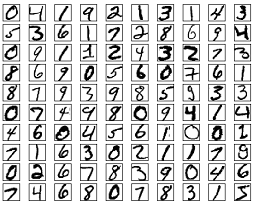
\includegraphics[width=0.733\textwidth]{images/mnist_100_digits.png}
\end{center}

\noindent 然后开发一个能够从这些训练样本中学习的系统. 换句话说，神经网络使用这些样本来自动推断识别手写数字的规则. 此外，通过增加训练样本的数量，网络可以学到更多关于手写的知识，从而提高其准确性. 所以虽然我上面只展示了 100 个训练数字，但也许我们可以通过使用数千甚至数百万或数十亿个训练样本来构建一个更好的手写识别器.

在本章中，我们将编写一个实现神经网络的计算机程序，该网络学习识别手写数字. 这个程序只有 74 行，并且不使用任何特殊的神经网络库. 但这个简短的程序可以在没有人工干预的情况下以超过 96\% 的准确率识别数字. 此外，在后面的章节中，我们将发展一些想法，可以将准确率提高到超过 99\%. 事实上，最好的商业神经网络现在如此之好，以至于银行用它们来处理支票，邮局用它们来识别地址.

我们专注于手写识别，因为它是学习神经网络的一个极好的原型问题. 作为一个原型，它恰好处于一个最佳位置：它具有挑战性——识别手写数字绝非易事——但它又没有难到需要极其复杂的解决方案或巨大的计算能力. 此外，它是发展更先进技术（如深度学习）的好方法. 因此，在整本书中我们将反复回到手写识别的问题上. 在本书后面，我们将讨论这些想法如何应用于计算机视觉中的其他问题，以及语音、自然语言处理和其他领域.

当然，如果本章的目的仅仅是编写一个识别手写数字的计算机程序，那么本章会短得多！但在过程中我们将发展许多关于神经网络的关键思想，包括两种重要类型的人工神经元\label{term:11}（感知机和 S 型神经元），以及神经网络的标准学习算法\label{term:12}，称为随机梯度\label{term:13}下降\label{term:10}\label{term:9}. 在整个过程中，我专注于解释\emph{为什么}事情要这样做，以及建立你的神经网络直觉. 这需要比仅仅展示基本机制更长的讨论，但为了你将获得的更深入理解，这是值得的. 其中的收获之一是，到本章结束时，我们将能够理解什么是深度学习，以及它为什么重要.
\sectionTitle{感知机}{感知机}

什么是神经网络？为了入门，我将解释一种称为\emph{感知机}（perceptron）\label{term:3}的人工神经元. 感知机由科学家 Frank Rosenblatt 在 20 世纪 50 年代和 60 年代开发，灵感来自 Warren McCulloch 和 Walter Pitts 的早期工作. 如今，使用其他人工神经元模型更为常见——在本书中，以及在许多现代神经网络工作中，使用的主要神经元模型是一种称为\emph{S 型神经元}（sigmoid neuron）\label{term:4}的模型. 我们很快就会讲到 S 型神经元. 但为了理解为什么 S 型神经元被如此定义，值得先花时间理解感知机.

那么感知机是如何工作的？感知机接受几个二进制输入，$x_1, x_2, \ldots$，并产生一个二进制输出：

\begin{center}
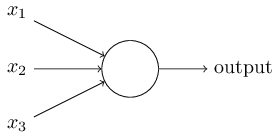
\includegraphics[width=0.9\textwidth]{images/tikz0.png}
\end{center}

\noindent 在所示的例子中，感知机有三个输入，$x_1, x_2, x_3$. 一般来说，它可能有更多或更少的输入.Rosenblatt 提出了一个简单的规则来计算输出. 他引入了权重\label{term:14}，$w_1,w_2,\ldots$，即表示各个输入对输出的重要性的实数. 神经元的输出，$0$ 或 $1$，取决于加权和 $\sum_j w_j x_j$ 是小于还是大于某个阈值\label{term:15}. 就像权重一样，阈值是一个实数，是神经元的一个参数. 用更精确的代数术语来说：

\begin{equation}
\mbox{output} = \left\{ \begin{array}{ll} 0 & \mbox{if } \sum_j w_j x_j \leq \mbox{ threshold} \\ 1 & \mbox{if } \sum_j w_j x_j > \mbox{ threshold} \end{array} \right.
\tag{1}
\end{equation}

\noindent 感知机的工作原理就是如此！

这就是基本的数学模型. 你可以把感知机看作是一种通过权衡证据来做出决策的设备. 让我举个例子. 这不是一个非常现实的例子，但它很容易理解，我们很快就会讲到更现实的例子. 假设周末快到了，你听说你的城市将举办一个奶酪节. 你喜欢奶酪，正在决定是否去参加这个节日. 你可能会通过权衡三个因素来做出决定：

\begin{enumerate}

\item 天气好吗？

\item 你的男朋友或女朋友想陪你吗？

\item 节日地点靠近公共交通吗？（你没有车）.

\end{enumerate}

我们可以用相应的二进制变量 $x_1, x_2$ 和 $x_3$ 来表示这三个因素. 例如，如果天气好，我们有 $x_1 = 1$，如果天气不好，$x_1 = 0$. 类似地，如果你的男朋友或女朋友想去，$x_2 = 1$，如果不想，$x_2 = 0$. 对于 $x_3$ 和公共交通也是如此.

现在，假设你非常喜欢奶酪，以至于即使你的男朋友或女朋友不感兴趣，而且节日地点很难到达，你也乐意去参加. 但也许你真的很讨厌坏天气，如果天气不好，你绝不会去参加节日. 你可以使用感知机来模拟这种决策. 一种方法是选择天气的权重 $w_1 = 6$，其他条件的权重 $w_2 = 2$ 和 $w_3 = 2$.$w_1$ 的较大值表明天气对你来说很重要，远比你男朋友或女朋友是否陪你，或公共交通是否近便更重要. 最后，假设你为感知机选择了阈值 $5$. 有了这些选择，感知机实现了所需的决策模型，每当天气好时输出 $1$，每当天气不好时输出 $0$. 你的男朋友或女朋友是否想去，或者公共交通是否在附近，对输出没有影响.

通过改变权重和阈值，我们可以得到不同的决策模型. 例如，假设我们改为选择阈值 $3$. 那么感知机将决定，只要天气好\emph{或}节日地点靠近公共交通\emph{且}你的男朋友或女朋友愿意陪你，你就应该去参加节日. 换句话说，这将是一个不同的决策模型. 降低阈值意味着你更愿意去参加节日.

显然，感知机并不是人类决策的完整模型！但这个例子说明的是感知机如何权衡不同种类的证据来做出决策. 而且，一个由感知机组成的复杂网络可以做出相当微妙的决策，这似乎是合理的：

\begin{center}
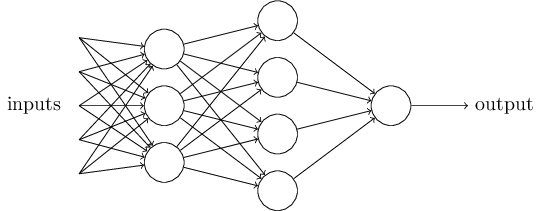
\includegraphics[width=0.9\textwidth]{images/tikz1.png}
\end{center}

\noindent 在这个网络中，第一列感知机——我们将称之为第一层感知机——通过权衡输入证据做出三个非常简单的决策. 第二层的感知机呢？这些感知机中的每一个都通过权衡第一层决策的结果来做出决策. 这样，第二层的感知机可以在比第一层感知机更复杂、更抽象的层次上做出决策. 而第三层的感知机可以做出更复杂的决策. 通过这种方式，一个多层的感知机网络可以进行复杂的决策.

顺便提一下，当我定义感知机时，我说感知机只有一个输出. 在上面的网络中，感知机看起来有多个输出. 事实上，它们仍然是单输出. 多个输出箭头仅仅是一种有用的方式，用来表示一个感知机的输出被用作其他几个感知机的输入. 这比画一条单一的输出线然后分叉要不那么笨拙.

让我们简化描述感知机的方式. 条件 $\sum_j w_j x_j > \mbox{threshold}$ 很繁琐，我们可以做两个符号上的改变来简化它. 第一个改变是将 $\sum_j w_j x_j$ 写成点积\label{term:16}，$w \cdot x \equiv \sum_j w_j x_j$，其中 $w$ 和 $x$ 是向量，其分量分别是权重和输入. 第二个改变是将阈值移到不等式的另一边，并用所谓的感知机的\emph{偏置}（bias）\label{term:5}代替它，$b \equiv -\mbox{threshold}$. 使用偏置代替阈值，感知机规则可以重写为：

\begin{equation}
\mbox{output} = \left\{ \begin{array}{ll} 0 & \mbox{if } w\cdot x + b \leq 0 \\ 1 & \mbox{if } w\cdot x + b > 0 \end{array} \right.
\tag{2}
\end{equation}

\noindent 你可以把偏置看作衡量让感知机输出 $1$ 有多容易的度量. 或者用更生物学的术语来说，偏置是衡量让感知机\emph{激发}有多容易的度量. 对于一个偏置非常大的感知机，它极容易输出 $1$. 但如果偏置非常负，那么感知机就很难输出 $1$. 显然，引入偏置只是我们描述感知机方式的一个小改变，但我们稍后会看到，它带来了进一步的符号简化. 因此，在本书的剩余部分，我们将不使用阈值，而是始终使用偏置.

我已经将感知机描述为一种权衡证据以做出决策的方法. 感知机的另一种用途是计算我们通常认为构成计算基础的基本逻辑函数，例如 \texttt{AND}、\texttt{OR} 和 \texttt{NAND}. 例如，假设我们有一个感知机，有两个输入，每个输入的权重为 $-2$，总偏置为 $3$. 这是我们的感知机：

\begin{center}
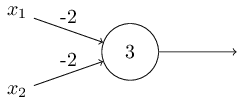
\includegraphics[width=0.9\textwidth]{images/tikz2.png}
\end{center}

\noindent 然后我们看到输入 $00$ 产生输出 $1$，因为 $(-2)*0+(-2)*0+3 = 3$ 是正的. 这里，我引入了 $*$ 符号来使乘法明确. 类似的计算表明，输入 $01$ 和 $10$ 产生输出 $1$. 但输入 $11$ 产生输出 $0$，因为 $(-2)*1+(-2)*1+3 = -1$ 是负的. 因此我们的感知机实现了一个 NAND 门！

\texttt{NAND} 的例子表明，我们可以使用感知机来计算简单的逻辑函数. 事实上，我们可以使用感知机网络来计算\emph{任何}逻辑函数. 原因是 \texttt{NAND} 门对于计算是通用的，也就是说，我们可以用 \texttt{NAND} 门构建任何计算. 例如，我们可以使用 \texttt{NAND} 门构建一个将两个比特 $x_1$ 和 $x_2$ 相加的电路. 这需要计算按位和 $x_1 \oplus x_2$，以及一个进位比特，当 $x_1$ 和 $x_2$ 都为 $1$ 时，该进位比特被设置为 $1$，即进位比特就是按位乘积 $x_1 x_2$：

\begin{center}
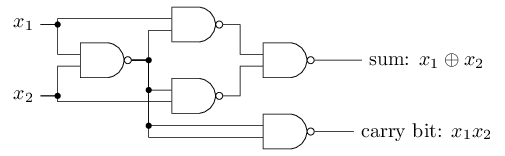
\includegraphics[width=0.9\textwidth]{images/tikz3.png}
\end{center}

\noindent 为了得到等效的感知机网络，我们将所有 NAND 门替换为具有两个输入的感知机，每个输入的权重为 $-2$，总偏置为 $3$. 这是得到的网络. 注意，我将对应于右下角 NAND 门的感知机稍微移动了一下，只是为了更容易在图上画箭头：

\begin{center}
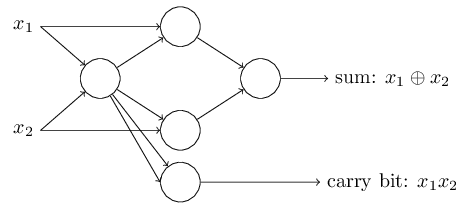
\includegraphics[width=0.9\textwidth]{images/tikz4.png}
\end{center}

\noindent 这个感知机网络的一个显著特点是，最左边感知机的输出被两次用作最底部感知机的输入. 当我定义感知机模型时，我没有说是否允许这种同一位置的双重输出. 实际上，这并不太重要. 如果我们不想允许这种事情，那么可以简单地将两条线合并为一条权重为 -4 的单一连接，而不是两条权重为 -2 的连接.（如果你觉得这不明显，你应该停下来向自己证明这是等价的.）有了这个改变，网络看起来如下，所有未标记的权重等于 -2，所有偏置等于 3，以及一个标记为 -4 的单一权重：

\begin{center}
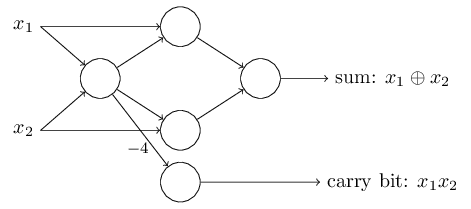
\includegraphics[width=0.9\textwidth]{images/tikz5.png}
\end{center}

\noindent 到目前为止，我一直将像 $x_1$ 和 $x_2$ 这样的输入画成漂浮在感知机网络左侧的变量. 事实上，按照惯例，我们会画一个额外的感知机层——输入层\label{term:17}——来编码输入：

\begin{center}
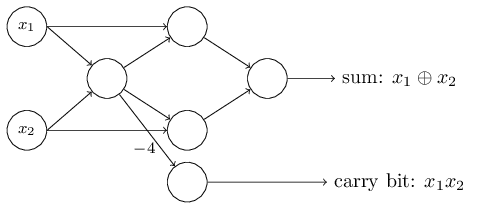
\includegraphics[width=0.9\textwidth]{images/tikz6.png}
\end{center}

\noindent 这种输入感知机的表示法，其中我们有一个输出，但没有输入，

\begin{center}
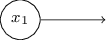
\includegraphics[width=0.9\textwidth]{images/tikz7.png}
\end{center}

\noindent 是一种简写. 它实际上并不意味着一个没有输入的感知机. 要看到这一点，假设我们确实有一个没有输入的感知机. 那么加权和 $\sum_j w_j x_j$ 将始终为零，因此如果 $b > 0$，感知机将输出 $1$，如果 $b \leq 0$，则输出 $0$. 也就是说，感知机将简单地输出一个固定值，而不是所需的值（在上面的例子中是 $x_1$）. 最好将输入感知机视为实际上根本不是感知机，而是特殊单元，它们被简单地定义为输出所需的值，$x_1, x_2,\ldots$.

加法器例子展示了如何使用感知机网络来模拟包含许多 \texttt{NAND} 门的电路. 而且因为 \texttt{NAND} 门对于计算是通用的，所以感知机对于计算也是通用的.

感知机的计算通用性既令人安心又令人失望. 它令人安心，因为它告诉我们感知机网络可以像任何其他计算设备一样强大. 但它也令人失望，因为它让人觉得感知机仅仅是一种新型的 \texttt{NAND} 门. 这算不上什么大新闻！

然而，情况比这种观点所暗示的要好. 事实证明，我们可以设计\emph{学习算法}，它可以自动调整人工神经元网络的权重和偏置. 这种调整是在响应外部刺激时发生的，没有程序员的直接干预. 这些学习算法使我们能够以一种与常规逻辑门截然不同的方式使用人工神经元. 我们的神经网络可以简单地学习解决问题，而不是明确地布置 \texttt{NAND} 和其他门的电路，有时这些问题直接设计常规电路会极其困难.
\sectionTitle{S 型神经元}{S 型神经元}

学习算法听起来很棒. 但我们如何为神经网络设计这样的算法呢？假设我们有一个感知机网络，想用它来学习解决某个问题. 例如，网络的输入可能是扫描的手写数字图像的原始像素数据. 我们希望网络学习权重和偏置，使得网络的输出能正确分类该数字. 为了了解学习可能如何工作，假设我们对网络中的某个权重（或偏置）做一个微小的改变. 我们希望的是，权重的这个微小改变只会引起网络输出的一个微小相应改变. 正如我们稍后将看到的，这一性质将使学习成为可能. 示意性地，这就是我们想要的（显然这个网络太简单，无法进行手写数字识别！）：

\begin{center}
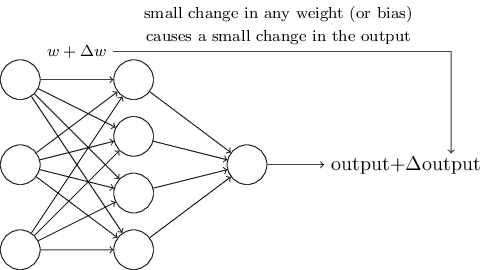
\includegraphics[width=0.9\textwidth]{images/tikz8.png}
\end{center}

\noindent 如果权重（或偏置）的微小改变只会引起输出的微小改变，那么我们就可以利用这一事实来修改权重和偏置，使网络的行为更符合我们的期望. 例如，假设网络错误地将一张图像分类为 ``8''，而它应该是 ``9''. 我们可以找出如何对权重和偏置做微小改变，使网络稍微更接近将图像分类为 ``9''. 然后我们重复这一过程，一次又一次地改变权重和偏置，以产生越来越好的输出. 网络就在学习了.

问题在于，当我们的网络包含感知机时，情况并非如此. 事实上，网络中任何单个感知机的权重或偏置的微小改变，有时会导致该感知机的输出完全翻转，比如从 $0$ 变为 $1$. 这种翻转随后可能导致网络其余部分的行为以某种非常复杂的方式完全改变. 因此，虽然你的 ``9'' 现在可能被正确分类了，但网络在所有其他图像上的行为很可能已经以某种难以控制的方式完全改变了. 这使得我们很难看到如何逐步修改权重和偏置，使网络更接近期望的行为. 也许有某种巧妙的方法可以绕过这个问题. 但如何让感知机网络学习并不是显而易见的.

我们可以通过引入一种新类型的人工神经元来克服这个问题，称为 S 型神经元. S 型神经元与感知机类似，但经过修改，使其权重和偏置的微小改变只会引起输出的微小改变. 这是关键事实，它将使 S 型神经元网络能够学习.

好的，让我来描述 S 型神经元. 我们将用与描述感知机相同的方式来描绘 S 型神经元：

\begin{center}
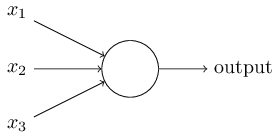
\includegraphics[width=0.9\textwidth]{images/tikz9.png}
\end{center}

\noindent 就像感知机一样，S 型神经元有输入，$x_1, x_2, \ldots$. 但这些输入不只是 $0$ 或 $1$，还可以取 $0$ 到 $1$ 之间的任意值. 例如，$0.638\ldots$ 是 S 型神经元的有效输入. 同样像感知机一样，S 型神经元对每个输入都有权重，$w_1, w_2, \ldots$，以及一个总偏置，$b$. 但输出不是 $0$ 或 $1$. 相反，它是 $\sigma(w \cdot x+b)$，其中 $\sigma$ 被称为 S 型函数\label{term:18} * *顺便说一句，$\sigma$ 有时被称为逻辑斯蒂函数\label{term:19}，这类新神经元被称为逻辑斯蒂神经元. 记住这个术语很有用，因为许多从事神经网络工作的人都使用这些术语. 不过，我们将坚持使用 S 型这一术语.，其定义为：

\begin{equation}
\sigma(z) \equiv \frac{1}{1+e^{-z}}.
\tag{3}
\end{equation}

\noindent 更明确地说，一个 S 型神经元在输入为 $x_1,x_2,\ldots$、权重为 $w_1,w_2,\ldots$、偏置为 $b$ 时的输出是

\begin{equation}
\frac{1}{1+\exp(-\sum_j w_j x_j-b)}.
\tag{4}
\end{equation}

\noindent 乍一看，S 型神经元与感知机看起来非常不同. 如果你还不熟悉 S 型函数，它的代数形式可能显得晦涩难懂. 事实上，感知机和 S 型神经元之间有许多相似之处，而 S 型函数的代数形式更多地是一个技术细节，而不是理解上的真正障碍.

为了理解与感知机模型的相似性，假设 $z \equiv w \cdot x + b$ 是一个很大的正数. 那么 $e^{-z} \approx 0$，因此 $\sigma(z) \approx 1$. 换句话说，当 $z = w \cdot x+b$ 很大且为正时，S 型神经元的输出近似为 $1$，就像感知机一样. 另一方面，假设 $z = w \cdot x+b$ 非常负. 那么 $e^{-z} \rightarrow \infty$，且 $\sigma(z) \approx 0$. 所以当 $z = w \cdot x +b$ 非常负时，S 型神经元的行为也密切近似于感知机. 只有当 $w \cdot x+b$ 的大小适中时，才会与感知机模型有较大偏差.

那么 $\sigma$ 的代数形式呢？我们如何理解它？事实上，$\sigma$ 的确切形式并不那么重要——真正重要的是函数绘制出来的形状. 形状如下：这个形状是阶梯函数平滑化后的版本：如果 $\sigma$ 实际上是一个阶梯函数，那么 S 型神经元就 \emph{是} 一个感知机，因为输出将是 $1$ 或 $0$，取决于 $w\cdot x+b$ 是正还是负*\footnote{实际上，当 $w \cdot x +b = 0$ 时，感知机输出 $0$，而阶梯函数输出 $1$. 所以严格来说，我们需要在那一点修改阶梯函数. 但你明白意思了.}. 通过使用实际的 $\sigma$ 函数，我们得到的是，如上文已经暗示的，一个平滑化的感知机. 事实上，正是 $\sigma$ 函数的平滑性才是关键事实，而不是它的具体形式. $\sigma$ 的平滑性意味着权重中的微小变化 $\Delta w_j$ 和偏置中的微小变化 $\Delta b$ 将产生神经元输出的微小变化 $\Delta \mbox{output}$. 事实上，微积分告诉我们 $\Delta \mbox{output}$ 可以很好地近似为

\begin{equation}
\Delta \mbox{output} \approx \sum_j \frac{\partial \, \mbox{output}}{\partial w_j} \Delta w_j + \frac{\partial \, \mbox{output}}{\partial b} \Delta b,
\tag{5}
\end{equation}

\noindent 其中求和是对所有
权重 $w_j$ 进行的，$\partial \, \mbox{output} / \partial w_j$ 和 $\partial \, \mbox{output} /\partial b$ 分别表示 $\mbox{output}$ 对 $w_j$ 和 $b$ 的偏导数\label{term:21}\label{term:20}. 如果你对偏导数不太熟悉，不要慌张！虽然上面的表达式看起来很复杂，有那么多偏导数，但它实际上说的是一件非常简单的事（而且是非常好的消息）：$\Delta \mbox{output}$ 是权重和偏置的变化 $\Delta w_j$ 和 $\Delta b$ 的 \emph{线性函数}. 这种线性关系使得我们可以很容易地选择权重和偏置的微小变化，以实现输出中任何期望的微小变化. 因此，虽然 S 型神经元在定性行为上与感知机有许多相同之处，但它们使我们更容易弄清楚改变权重和偏置将如何改变输出.

如果真正重要的是 $\sigma$ 的形状，而不是它的确切形式，那么为什么要使用方程 (3) 中 $\sigma$ 所用的特定形式

\begin{align*}
\sigma(z) \equiv \frac{1}{1+e^{-z}} \nonumber
\end{align*}

\noindent 呢？事实上，在本书后面，我们偶尔会考虑输出为 $f(w \cdot x + b)$ 的神经元，其中 $f(\cdot)$ 是某种其他的 \emph{激活函数}. 当我们使用不同的激活函数时，主要的变化是方程 (5) 中偏导数的具体值

\begin{align*}
\Delta \mbox{output} \approx \sum_j \frac{\partial \, \mbox{output}}{\partial w_j} \Delta w_j + \frac{\partial \, \mbox{output}}{\partial b} \Delta b \nonumber
\end{align*}

\noindent 会改变. 事实证明，当我们稍后计算这些偏导数时，使用 $\sigma$ 将简化代数运算，这仅仅是因为指数函数在微分时具有优美的性质. 无论如何，$\sigma$ 在神经网络研究中被广泛使用，并且是我们在本书中最常使用的激活函数\label{term:22}.

我们应该如何解释 S 型神经元的输出？显然，感知机和 S 型神经元之间的一个重大区别是，S 型神经元不只输出 $0$ 或 $1$. 它们可以输出 $0$ 到 $1$ 之间的任何实数，因此像 $0.173\ldots$ 和 $0.689\ldots$ 这样的值都是合法的输出. 这可能很有用，例如，如果我们想用输出值来表示输入到神经网络的图像中像素的平均强度. 但有时它也可能带来麻烦. 假设我们希望网络的输出表明 ``输入图像是 9'' 或 ``输入图像不是 9''. 显然，如果输出是 $0$ 或 $1$，就像感知机那样，做这件事会最容易. 但在实践中，我们可以建立一个约定来处理这个问题，例如，决定将任何至少为 $0.5$ 的输出解释为表示 ``9''，而将任何小于 $0.5$ 的输出解释为表示 ``不是 9''. 当我们使用这样的约定时，我总会明确说明，因此它不应该引起任何混淆.

\begin{exerciseBox}{练习}

\begin{itemize}

\item \textbf{模拟感知机的 S 型神经元，第一部分} $\mbox{}$ \\ 假设我们取一个感知机网络中的所有
权重和偏置，并将它们乘以一个正常数 $c > 0$. 证明网络的行为不变.

\item \textbf{模拟感知机的 S 型神经元，第二部分} $\mbox{}$ \\ 假设我们有与上一题相同的设置——一个感知机网络. 还假设感知机网络的整体输入已经选定. 我们不需要实际的输入值，只需要输入已经固定. 假设权重和偏置使得对于网络中任何特定感知机的输入 $x$，都有 $w \cdot x + b \neq 0$. 现在将网络中的所有感知机替换为 S 型神经元，并将权重和偏置乘以一个正常数 $c > 0$. 证明当 $c \rightarrow \infty$ 时，这个 S 型神经元网络的行为与感知机网络完全相同. 当其中一个感知机满足 $w \cdot x + b = 0$ 时，这为什么会失效？

\end{itemize}

\end{exerciseBox}
\sectionTitle{神经网络的结构}{神经网络的结构}

在下一节中，我将介绍一个能够相当出色地分类手写数字的神经网络. 为了做好准备，先解释一些术语会有所帮助，这些术语让我们能够命名网络的不同部分. 假设我们有这样一个网络：

\begin{center}
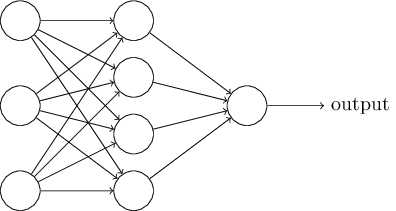
\includegraphics[width=0.9\textwidth]{images/tikz10.png}
\end{center}

\noindent 如前所述，这个网络中最左边的一层称为输入层，该层内的神经元称为输入神经元. 最右边的一层，即输出层\label{term:23}，包含输出神经元，或者像本例中那样，只包含一个输出神经元. 中间层称为隐藏层\label{term:24}，因为这一层中的神经元既不是输入也不是输出. ``隐藏''这个词听起来可能有点神秘——我第一次听到这个词时，以为它一定有什么深刻的哲学或数学意义——但它实际上只不过意味着``既不是输入也不是输出''. 上面的网络只有一个隐藏层，但有些网络有多个隐藏层. 例如，下面这个四层网络有两个隐藏层：

\begin{center}
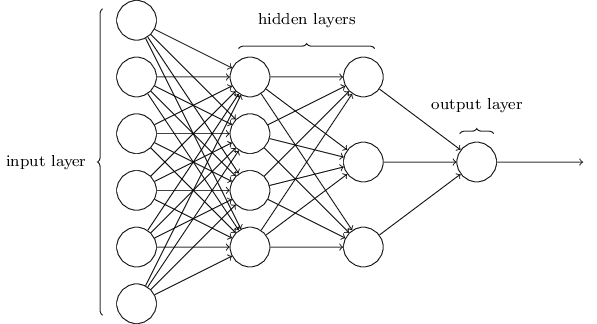
\includegraphics[width=0.9\textwidth]{images/tikz11.png}
\end{center}

\noindent 有点令人困惑的是，由于历史原因，这种多层网络有时被称为多层感知机或 MLP，尽管它们是由 S 型神经元而非感知机构成的. 我在这本书中不会使用 MLP 这个术语，因为我认为它容易引起混淆，但想提醒你它的存在.

网络中输入层和输出层的设计通常很直接. 例如，假设我们要判断一张手写图像是否描绘了一个``9''. 设计网络的一种自然方式是将图像像素的强度编码到输入神经元中. 如果图像是一张 $64$ 乘 $64$ 的灰度图像，那么我们会有 $4,096 = 64 \times 64$ 个输入神经元，其强度被适当地缩放到 $0$ 和 $1$ 之间. 输出层将只包含一个神经元，输出值小于 $0.5$ 表示``输入图像不是 9''，大于 $0.5$ 表示``输入图像是 9''.

虽然神经网络的输入层和输出层的设计通常很直接，但隐藏层的设计却可能相当有艺术性. 特别是，无法用几条简单的经验法则来概括隐藏层的设计过程. 相反，神经网络研究人员已经为隐藏层发展出了许多设计启发式方法，这些方法帮助人们从他们的网络中获得想要的行为. 例如，这类启发式方法可以用来帮助确定如何在隐藏层的数量和训练网络所需的时间之间进行权衡. 我们将在本书后面遇到几种这样的设计启发式方法.

到目前为止，我们讨论的都是这样一类神经网络：其中一层的输出被用作下一层的输入. 这样的网络被称为\emph{前馈}神经网络. 这意味着网络中没有环路——信息总是向前馈送，从不向后反馈. 如果我们确实有环路，就会出现 $\sigma$ 函数的输入依赖于输出的情况. 那将很难理解，所以我们不允许这样的环路.

然而，还有其他类型的人工神经网络模型，其中反馈环路是可能的. 这些模型被称为循环神经网络\label{term:25}. 这些模型中的想法是让神经元在有限的一段时间内激活，然后进入静息状态. 这种激活可以刺激其他神经元，这些神经元可能稍后也会激活一段时间. 这又会导致更多的神经元激活，因此随着时间的推移，我们会得到一连串激活的神经元. 在这样的模型中，环路不会引起问题，因为一个神经元的输出只会在稍后的时间影响其输入，而不是瞬时影响.

循环神经网络的影响力不如前馈\label{term:26}网络，部分原因是循环网络的学习算法（至少到目前为止）不够强大. 但循环网络仍然极其有趣. 它们在精神上比前馈网络更接近我们大脑的工作方式. 而且循环网络有可能解决那些前馈网络极难解决的重要问题. 然而，为了限制我们的范围，在本书中我们将集中讨论使用更广泛的前馈网络.
\sectionTitle{一个识别手写数字的简单网络}{一个识别手写数字的简单网络}

定义了神经网络之后，让我们回到手写数字识别. 我们可以把识别手写数字的问题拆分成两个子问题. 首先，我们需要一种方法，把一张包含多个数字的图像拆分成一系列单独的图像，每张图像只包含一个数字. 例如，我们希望把图像

\begin{center}

\includegraphics[width=0.500\textwidth]{images/digits.png}
\end{center}

\noindent 拆分成六张单独的图像，

\begin{center}

\includegraphics[width=0.733\textwidth]{images/digits_separate.png}
\end{center}

\noindent 我们人类可以轻松地解决这个\emph{分割问题}（segmentation problem）\label{term:6}，但对计算机程序来说，正确地拆分图像却颇具挑战性. 一旦图像被分割开，程序就需要对每个单独的数字进行分类. 例如，我们希望程序能够识别出上面第一张图像

\begin{center}

\includegraphics[width=0.107\textwidth]{images/mnist_first_digit.png}
\end{center}

\noindent 是一个 5.

我们将专注于编写一个程序来解决第二个问题，也就是对单个数字进行分类. 我们这样做是因为，一旦你有了对单个数字进行分类的好方法，分割问题其实并不那么难解决. 解决分割问题有很多方法. 一种方法是尝试许多不同的图像分割方式，用单个数字分类器为每种尝试的分割打分. 如果单个数字分类器对各个分割段中的分类都很有信心，那么这种尝试的分割就得到高分；如果分类器在一个或多个分割段中遇到很大困难，那么就得到低分. 其想法是，如果分类器在某处遇到困难，那么很可能是因为分割方式选择得不正确. 这个想法以及其他变体可以用来相当好地解决分割问题. 所以，与其操心分割问题，我们不如集中精力开发一个神经网络，来解决更有趣也更困难的问题，即识别单个手写数字.

为了识别单个数字，我们将使用一个三层神经网络：

\begin{center}
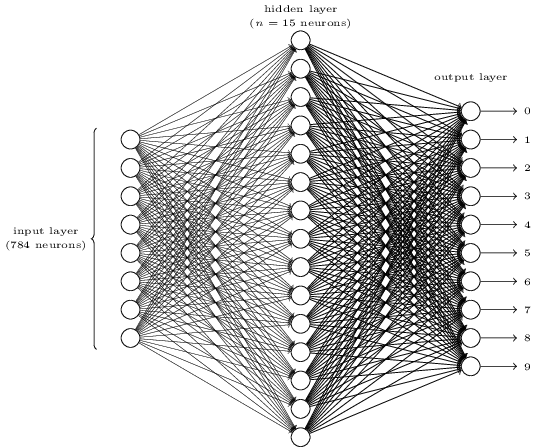
\includegraphics[width=0.9\textwidth]{images/tikz12.png}
\end{center}

\noindent 网络的输入层包含对输入像素值进行编码的神经元. 正如下一节将要讨论的，我们用于训练网络的数据将由许多 $28$ 乘 $28$ 像素的扫描手写数字图像组成，因此输入层包含 $784 = 28 \times 28$ 个神经元. 为简单起见，我在上图中省略了 $784$ 个输入神经元中的大部分. 输入像素是灰度的，值 $0.0$ 表示白色，值 $1.0$ 表示黑色，介于两者之间的值表示逐渐变暗的灰色.

网络的第二层是一个隐藏层. 我们用 $n$ 表示这个隐藏层中神经元的数量，并将尝试不同的 $n$ 值. 图中所示的例子展示了一个很小的隐藏层，只包含 $n = 15$ 个神经元.

网络的输出层包含 10 个神经元. 如果第一个神经元激活，即输出 $\approx 1$，那么这表明网络认为该数字是 $0$. 如果第二个神经元激活，那么这表明网络认为该数字是 $1$. 依此类推. 更精确一点说，我们把输出神经元从 $0$ 到 $9$ 编号，然后找出哪个神经元的激活值\label{term:27}最高. 如果那个神经元是，比如说，编号为 $6$ 的神经元，那么我们的网络就会猜测输入的数字是 $6$. 对其他输出神经元也依此类推.

你可能会想，为什么我们要使用 $10$ 个输出神经元. 毕竟，网络的目标是告诉我们输入图像对应哪个数字（$0, 1, 2, \ldots, 9$）. 一种看似自然的方式是只使用 $4$ 个输出神经元，把每个神经元看作取一个二值，取决于该神经元的输出更接近 $0$ 还是更接近 $1$. 四个神经元足以编码答案，因为 $2^4 = 16$ 大于输入数字的 10 个可能取值. 为什么我们的网络反而要使用 $10$ 个神经元呢？这不是很低效吗？最终的理由是经验性的：我们可以把两种网络设计都试一下，结果发现，对于这个特定的问题，使用 $10$ 个输出神经元的网络比使用 $4$ 个输出神经元的网络学得更好. 但这让我们不禁想问，\emph{为什么}使用 $10$ 个输出神经元效果更好. 有没有某种启发式方法能事先告诉我们，应该使用 $10$ 输出的编码而不是 $4$ 输出的编码？

要理解我们为什么这样做，从基本原理出发思考神经网络在做什么会有所帮助. 先考虑我们使用 $10$ 个输出神经元的情况. 让我们把注意力集中在第一个输出神经元上，也就是那个试图判断数字是不是 $0$ 的神经元. 它通过权衡来自隐藏层神经元的证据来做到这一点. 那些隐藏神经元在做什么呢？好吧，不妨为了讨论起见假设隐藏层中的第一个神经元检测如下图像是否存在：

\begin{center}

\includegraphics[width=0.217\textwidth]{images/mnist_top_left_feature.png}
\end{center}

\noindent 它可以通过给与该图像重叠的输入像素赋予很大的权重，而只给其他输入赋予很小的权重来做到这一点. 类似地，不妨为了讨论起见假设隐藏层中的第二、第三和第四个神经元检测如下图像是否存在：

\begin{center}
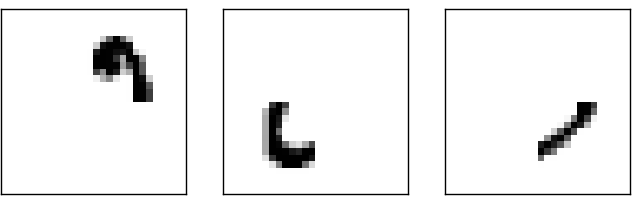
\includegraphics[width=0.707\textwidth]{images/mnist_other_features.png}
\end{center}

\noindent 你可能已经猜到了，这四张图像合在一起就构成了我们之前在那行数字中看到的 $0$ 图像：

\begin{center}

\includegraphics[width=0.217\textwidth]{images/mnist_complete_zero.png}
\end{center}

\noindent 所以，如果这四个隐藏神经元都激活，那么我们就可以得出结论：该数字是 $0$. 当然，这并不是我们用来断定图像是 $0$ 的\emph{唯一}证据 - 我们还可以通过许多其他方式合理地得到 $0$（比如，通过上述图像的平移，或轻微的变形）. 但至少在这个例子中，我们可以有把握地说，我们会断定输入是 $0$.

假设神经网络以这种方式运作，我们就能为为什么网络有 $10$ 个输出比有 $4$ 个输出更好给出一个合理的解释. 如果我们有 $4$ 个输出，那么第一个输出神经元将试图判断该数字的最高有效位是什么. 而要把那个最高有效位与上面所示的简单形状联系起来，并没有容易的办法. 很难想象数字的组成形状会与（比如说）输出中的最高有效位有任何好的历史性关联.

话虽如此，这一切都只是一种启发式. 没有什么规定说三层神经网络必须按我描述的方式运作，让隐藏神经元检测简单的组成形状. 也许某个聪明的学习算法会找到某种权重分配，让我们只使用 $4$ 个输出神经元. 但作为一种启发式，我所描述的这种思考方式相当有效，并且可以在设计好的神经网络结构时为你节省大量时间.

\begin{exerciseBox}{练习}

\begin{itemize}

\item 有一种方法可以通过在上面的三层网络中增加一个额外的层来确定数字的按位表示. 这个额外的层把前一层的输出转换成二进制表示，如下图所示. 为新的输出层找出一组权重和偏置. 假设前 $3$ 层神经元使得第三层（即旧的输出层）中正确输出的激活值至少为 $0.99$，而不正确输出的激活值小于 $0.01$.

\end{itemize}

\begin{center}
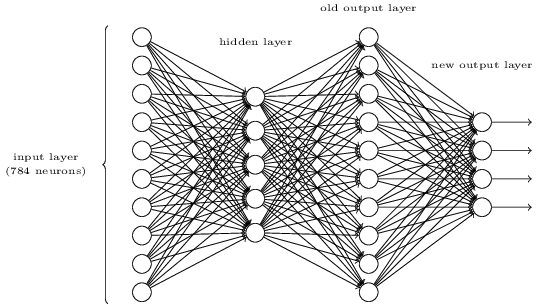
\includegraphics[width=0.9\textwidth]{images/tikz13.png}
\end{center}

\end{exerciseBox}
\sectionTitle{用梯度下降进行学习}{用梯度下降进行学习}

现在我们已经为神经网络设计好了结构，它如何学习识别数字呢？我们首先需要的是一个用于学习的数据集——即所谓的训练数据\label{term:28}集. 我们将使用 MNIST 数据集，其中包含数万张手写数字的扫描图像，以及它们正确的分类.MNIST 这个名字来源于它是 NIST（美国国家标准与技术研究院）收集的两个数据集的修改子集. 下面是 MNIST 中的几张图像：

\begin{center}

\includegraphics[width=0.700\textwidth]{images/digits_separate.png}
\end{center}

\noindent 如你所见，这些数字实际上与本章开头作为识别挑战展示的那些数字相同. 当然，在测试我们的网络时，我们会让它识别不在训练集\label{term:29}中的图像！

MNIST 数据分为两部分. 第一部分包含 60,000 张图像，用作训练数据. 这些图像是来自 250 人的手写样本扫描件，其中一半是美国人口普查局的员工，一半是高中生. 图像是灰度的，大小为 28 乘 28 像素.MNIST 数据集的第二部分是 10,000 张图像，用作测试数据\label{term:30}. 同样，这些是 28 乘 28 的灰度图像. 我们将使用测试数据来评估我们的神经网络学习识别数字的效果. 为了使其成为对性能的良好测试，测试数据取自与原始训练数据\emph{不同}的 250 人（尽管仍然是在人口普查局员工和高中生之间划分的群体）. 这有助于让我们相信，我们的系统能够识别那些在训练期间未见过其笔迹的人所写的数字.

我们将使用符号 $x$ 来表示一个训练输入. 将每个训练输入 $x$ 视为一个 $28 \times 28 = 784$ 维向量\label{term:31}会很方便. 向量中的每个条目代表图像中单个像素的灰度值. 我们将相应的期望输出记为 $y = y(x)$，其中 $y$ 是一个 $10$ 维向量. 例如，如果某个特定的训练图像 $x$ 描绘的是 $6$，那么 $y(x) = (0, 0, 0, 0, 0, 0, 1, 0, 0, 0)^T$ 就是网络期望的输出. 注意这里的 $T$ 是转置操作，将行向量转换为普通的（列）向量.

我们想要的是一个算法，它能让我们找到权重和偏置，使得对于所有训练输入 $x$，网络的输出都近似于 $y(x)$. 为了量化我们实现这一目标的程度，我们定义一个\emph{代价函数}*\footnote{有时也被称为\emph{损失}函数或\emph{目标}函数. 在本书中我们使用代价函数这一术语，但你应该注意其他术语，因为它们经常出现在研究论文和其他关于神经网络的讨论中.}：

\begin{equation}
C(w,b) \equiv \frac{1}{2n} \sum_x \| y(x) - a\|^2.
\tag{6}
\end{equation}

\noindent 这里，$w$ 表示网络中所有\emph{权重}的集合，$b$ 表示所有\emph{偏置}，$n$ 是训练输入的总数，$a$ 是当输入为 $x$ 时网络的输出向量，求和是对所有训练输入 $x$ 进行的. 当然，输出 $a$ 依赖于 $x$、$w$ 和 $b$，但为了保持符号简洁，我没有明确表示这种依赖关系. 符号 $\| v \|$ 只是表示向量 $v$ 的通常长度函数. 我们将 $C$ 称为\emph{二次}代价函数\label{term:32}；它有时也被称为\emph{均方误差}或简称 \emph{MSE}. 观察二次代价\label{term:33}函数的形式，我们看到 $C(w,b)$ 是非负的，因为求和中的每一项都是非负的. 此外，当对于所有训练输入 $x$，$y(x)$ 都近似等于输出 $a$ 时，代价 $C(w,b)$ 恰好变得很小，即 $C(w,b) \approx 0$. 因此，如果我们的训练算法\label{term:34}能够找到权重和偏置使得 $C(w,b) \approx 0$，那么它就做得很好. 相反，当 $C(w,b)$ 很大时，它就做得不太好——那意味着对于大量输入，$y(x)$ 并不接近输出 $a$. 因此，我们训练算法的目标将是最小化作为权重和偏置函数的代价 $C(w,b)$. 换句话说，我们想要找到一组使代价尽可能小的权重和偏置. 我们将使用一种称为\emph{梯度下降}的算法来实现这一点.

为什么要引入二次代价？毕竟，我们主要感兴趣的不是网络正确分类的图像数量吗？为什么不直接尝试最大化那个数量，而是最小化像二次代价这样的代理指标呢？问题在于，正确分类的图像数量并不是网络中权重和偏置的光滑函数. 在大多数情况下，对权重和偏置进行微小改变根本不会导致正确分类的训练图像数量发生任何变化. 这使得我们很难弄清楚如何改变权重和偏置来提高性能. 如果我们改用像二次代价这样的光滑代价函数，那么就容易弄清楚如何对权重和偏置进行微小改变，从而改善代价. 这就是为什么我们首先关注最小化二次代价，之后才会考察分类准确率.

即使我们想要使用光滑的代价函数，你可能仍然想知道为什么我们选择方程 (6) 中使用的二次函数

\begin{align*}
C(w,b) \equiv \frac{1}{2n} \sum_x \| y(x) - a\|^2 \nonumber
\end{align*}

\noindent. 这不是一个相当\emph{特设}的选择吗？也许如果我们选择不同的代价函数，我们会得到一组完全不同的最小化权重和偏置？这是一个合理的担忧，稍后我们会重新审视代价函数，并做一些修改. 然而，方程 (6) 中的二次代价函数

\begin{align*}
C(w,b) \equiv \frac{1}{2n} \sum_x \| y(x) - a\|^2 \nonumber
\end{align*}

\noindent 对于理解神经网络学习的基础知识来说完全够用，所以我们现在就坚持使用它.

回顾一下，我们训练神经网络的目标是找到使二次代价函数 $C(w, b)$ 最小化的权重和偏置. 这是一个适定问题，但就目前的形式而言，它有很多分散注意力的结构——将 $w$ 和 $b$ 解释为权重和偏置，背景中潜伏的 $\sigma$ 函数，网络结构的选择，MNIST，等等. 事实证明，通过忽略大部分这些结构，只专注于最小化方面，我们可以理解大量内容. 所以现在我们要忘记代价函数的具体形式、与神经网络的联系等等. 相反，我们将想象我们只是被给定了许多变量的一个函数，我们想要最小化那个函数. 我们将发展一种称为\emph{梯度下降}的技术，它可以用来解决这类最小化问题. 然后我们再回到我们想要为神经网络最小化的具体函数.

好的，假设我们试图最小化某个函数 $C(v)$. 这可以是许多变量的任何实值函数，$v = v_1, v_2, \ldots$. 注意我已经用 $v$ 替换了 $w$ 和 $b$ 的记号，以强调这可以是任何函数——我们不再特别在神经网络的背景下思考. 为了最小化 $C(v)$，将 $C$ 想象成仅有两个变量的函数会有所帮助，我们将这两个变量称为 $v_1$ 和 $v_2$：

\begin{center}
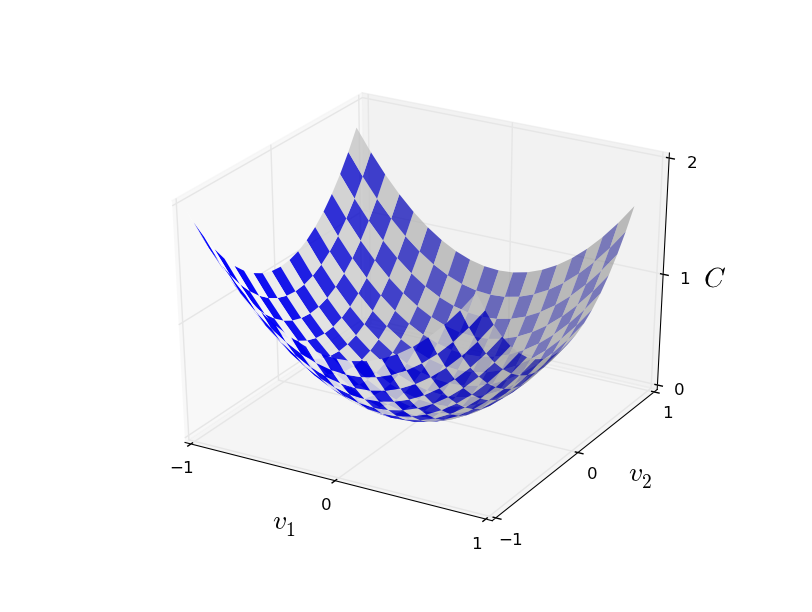
\includegraphics[width=0.903\textwidth]{images/valley.png}
\end{center}

\noindent 我们想要找到 $C$ 达到其全局最小值的位置. 当然，对于上面绘制的函数，我们可以目测图形并找到最小值. 从这个意义上说，我可能展示了一个稍微\emph{过于}简单的函数！一个一般的函数 $C$ 可能是许多变量的复杂函数，通常不可能仅仅通过目测图形来找到最小值.

解决这个问题的一种方法是使用微积分来尝试解析地找到最小值. 我们可以计算导数，然后尝试用它们来找到 $C$ 取极值的位置. 如果运气好的话，当 $C$ 只是一个或几个变量的函数时，这可能行得通. 但当我们有更多变量时，这将变成一场噩梦. 而对于神经网络，我们通常想要\emph{远}更多的变量——最大的神经网络的代价函数以极其复杂的方式依赖于数十亿的权重和偏置. 使用微积分来最小化那根本行不通！（在断言我们将通过将 $C$ 想象成仅有两个变量的函数来获得洞察力之后，我在两段话中两次转身说，“嘿，但如果它是远多于两个变量的函数呢？”对此我很抱歉. 请相信我，将 $C$ 想象成两个变量的函数确实有帮助. 只是有时那幅图景会失效，而最后两段话就是在处理这种失效. 好的数学思考往往涉及同时处理多个直观图景，学会何时适合使用每个图景，何时不适合.）

好的，所以微积分行不通. 幸运的是，有一个漂亮的类比暗示了一种效果相当好的算法. 我们首先将我们的函数想象成一种山谷. 如果你稍微眯眼看上面的图，那应该不难. 我们想象一个球沿着山谷的斜坡滚下. 我们的日常经验告诉我们，球最终会滚到谷底. 也许我们可以用这个想法作为找到函数最小值的方法？我们会随机选择一个（假想的）球的起点，然后模拟球滚到谷底的运动. 我们可以简单地通过计算 $C$ 的导数（也许还有一些二阶导数）来进行这种模拟——这些导数会告诉我们关于山谷局部“形状”所需的一切信息，从而告诉我们球应该如何滚动.

基于我刚才写的内容，你可能会认为我们将尝试写下球的牛顿运动方程，考虑摩擦和重力等的影响. 实际上，我们不会那么认真地对待滚球的类比——我们是在设计一种最小化 $C$ 的算法，而不是开发物理定律的精确模拟！球的视角是为了激发我们的想象力，而不是限制我们的思考. 所以，与其陷入物理学的所有混乱细节，不如简单地问自己：如果我们被宣布为一天的神，可以制定自己的物理定律，指示球应该如何滚动，我们可以选择什么运动定律，使得球总是滚到谷底？

为了使这个问题更精确，让我们思考一下当我们在 $v_1$ 方向上将球移动一小段 $\Delta v_1$，在 $v_2$ 方向上将球移动一小段 $\Delta v_2$ 时会发生什么. 微积分告诉我们 $C$ 的变化如下：

\begin{equation}
\Delta C \approx \frac{\partial C}{\partial v_1} \Delta v_1 + \frac{\partial C}{\partial v_2} \Delta v_2.
\tag{7}
\end{equation}

\noindent 我们将找到一种选择 $\Delta v_1$ 和 $\Delta v_2$ 的方法，使得 $\Delta C$ 为负；即，我们将选择它们使得球向谷底滚下. 为了弄清楚如何做出这样的选择，定义 $\Delta v$ 为 $v$ 中变化的向量会有所帮助，$\Delta v \equiv (\Delta v_1, \Delta v_2)^T$，其中 $T$ 同样是转置操作，将行向量转换为列向量. 我们还将 $C$ 的\emph{梯度}定义为偏导数的向量，$\left(\frac{\partial C}{\partial v_1}, \frac{\partial C}{\partial v_2}\right)^T$. 我们用 $\nabla C$ 表示梯度向量，即：

\begin{equation}
\nabla C \equiv \left( \frac{\partial C}{\partial v_1}, \frac{\partial C}{\partial v_2} \right)^T.
\tag{8}
\end{equation}

\noindent 稍后我们将用 $\Delta v$ 和梯度 $\nabla C$ 来重写变化 $\Delta C$. 但在那之前，我想澄清一些有时会让人对梯度感到困惑的事情. 当第一次遇到 $\nabla C$ 记号时，人们有时会想知道应该如何思考 $\nabla$ 符号.$\nabla$ 到底是什么意思？事实上，将 $\nabla C$ 视为一个单一的数学对象——上面定义的向量——是完全没问题的，它恰好用两个符号来书写. 从这个观点来看，$\nabla$ 只是一点记号上的旗帜挥舞，告诉你“嘿，$\nabla C$ 是一个梯度向量”. 还有更高级的观点，其中 $\nabla$ 可以被视为一个独立的数学实体（例如，作为一个微分算子），但我们不需要这样的观点.

有了这些定义，表达式 (7)
\begin{align*}
\Delta C \approx \frac{\partial C}{\partial v_1} \Delta v_1 + \frac{\partial C}{\partial v_2} \Delta v_2 \nonumber
\end{align*}

\noindent $\Delta C$ 可以改写为

\begin{equation}
\Delta C \approx \nabla C \cdot \Delta v.
\tag{9}
\end{equation}

\noindent 这个方程有助于解释为什么 $\nabla C$ 被称为梯度向量：$\nabla C$ 将 $v$ 的变化与 $C$ 的变化联系起来，正如我们对一个被称为梯度的东西所期望的那样. 但这个方程真正令人兴奋的地方在于，它让我们看到如何选择 $\Delta v$ 以使 $\Delta C$ 为负. 特别地，假设我们选择

\begin{equation}
\Delta v = -\eta \nabla C,
\tag{10}
\end{equation}

\noindent 其中 $\eta$ 是一个小的正参数（被称为\emph{学习率}）. 那么方程 (9)

\begin{align*}
\Delta C \approx \nabla C \cdot \Delta v \nonumber
\end{align*}

\noindent 告诉我们 $\Delta C \approx -\eta \nabla C \cdot \nabla C = -\eta \|\nabla C\|^2$. 因为 $\| \nabla C \|^2 \geq 0$，这保证了 $\Delta C \leq 0$，即如果我们按照 (10) 中的规定改变 $v$，$C$ 将始终减小，永不增大

\begin{align*}
\Delta v = -\eta \nabla C \nonumber
\end{align*}

\noindent. （当然，这是在方程 (9) 近似的限度内

\begin{align*}
\Delta C \approx \nabla C \cdot \Delta v \nonumber
\end{align*}

\noindent ）. 这正是我们想要的属性！因此我们将用方程 (10)

\begin{align*}
\Delta v = -\eta \nabla C \nonumber
\end{align*}

\noindent 来定义梯度下降算法中小球的``运动定律''. 也就是说，我们将使用方程 (10)

\begin{align*}
\Delta v = -\eta \nabla C \nonumber
\end{align*}

\noindent 来计算 $\Delta v$ 的值，然后将小球的位置 $v$ 移动该数量：

\begin{equation}
v \rightarrow v' = v -\eta \nabla C.
\tag{11}
\end{equation}

\noindent 然后我们再次使用这个更新规则，进行另一次移动. 如果我们一遍又一遍地这样做，我们将不断减小 $C$，直到——我们希望——达到一个全局最小值.

总结起来，梯度下降算法的工作方式是反复计算梯度 $\nabla C$，然后向\emph{相反}方向移动，``滚下''山谷的斜坡. 我们可以这样可视化它：

\begin{center}
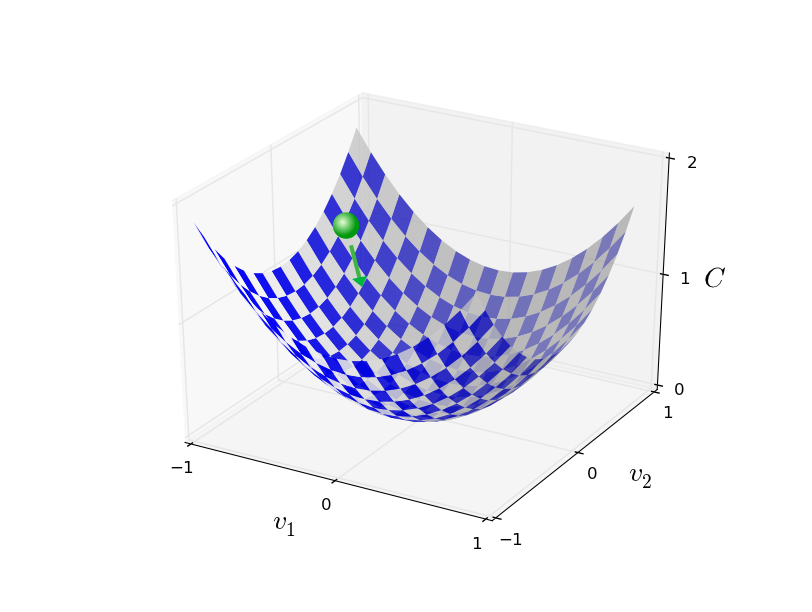
\includegraphics[width=0.903\textwidth]{images/valley_with_ball.png}
\end{center}

\noindent 注意，使用这个规则，梯度下降并不再现真实的物理运动. 在现实生活中，小球具有动量\label{term:35}，这种动量可能使它滚过斜坡，甚至（暂时地）滚上坡. 只有在摩擦效应起作用之后，小球才保证滚入山谷. 相比之下，我们选择 $\Delta v$ 的规则只是说``现在就往下走''. 对于寻找最小值来说，这仍然是一个相当不错的规则！

为了使梯度下降正确工作，我们需要选择学习率\label{term:36} $\eta$ 足够小，使得方程 (9)

\begin{align*}
\Delta C \approx \nabla C \cdot \Delta v \nonumber
\end{align*}

\noindent 是一个好的近似. 如果不这样做，我们可能最终得到 $\Delta C > 0$，这显然不好！同时，我们也不希望 $\eta$ 太小，因为那会使变化量 $\Delta v$ 非常微小，从而使梯度下降算法工作得非常缓慢. 在实际实现中，$\eta$ 经常被调整，以使方程 (9)

\begin{align*}
\Delta C \approx \nabla C \cdot \Delta v \nonumber
\end{align*}

\noindent 保持为一个好的近似，但算法又不会太慢. 我们稍后会看到这是如何工作的.

我已经解释了当 $C$ 只是两个变量的函数时的梯度下降. 但实际上，即使 $C$ 是更多变量的函数，一切也同样适用. 特别地，假设 $C$ 是 $m$ 个变量 $v_1,\ldots,v_m$ 的函数. 那么由微小变化 $\Delta v = (\Delta v_1, \ldots, \Delta v_m)^T$ 产生的 $C$ 的变化 $\Delta C$ 为

\begin{equation}
\Delta C \approx \nabla C \cdot \Delta v,
\tag{12}
\end{equation}

\noindent 其中梯度 $\nabla C$ 是向量

\begin{equation}
\nabla C \equiv \left(\frac{\partial C}{\partial v_1}, \ldots, \frac{\partial C}{\partial v_m}\right)^T.
\tag{13}
\end{equation}

\noindent 正如两变量的情况一样，我们可以选择

\begin{equation}
\Delta v = -\eta \nabla C,
\tag{14}
\end{equation}

\noindent 并且我们保证我们的（近似）表达式 (12)

\begin{align*}
\Delta C \approx \nabla C \cdot \Delta v \nonumber
\end{align*}

\noindent 对于 $\Delta C$ 将是负的. 这给了我们一种沿着梯度到达最小值的方法，即使 $C$ 是许多变量的函数，通过反复应用更新规则

\begin{equation}
v \rightarrow v' = v-\eta \nabla C.
\tag{15}
\end{equation}

\noindent 你可以把这个更新规则看作是在\emph{定义}梯度下降算法. 它给了我们一种反复改变位置 $v$ 以找到函数 $C$ 的最小值的方法. 这个规则并不总是有效——有几件事可能出错并阻止梯度下降找到 $C$ 的全局最小值，这一点我们将在后面的章节中回来探讨. 但在实践中，梯度下降通常工作得非常好，在神经网络中我们会发现它是最小化代价函数、从而帮助网络学习的一种强大方法.

事实上，从某种意义上说，梯度下降甚至是搜索最小值的\emph{最优}策略. 让我们假设我们试图在位置上移动 $\Delta v$ 以尽可能多地减小 $C$. 这等价于最小化 $\Delta C \approx \nabla C \cdot \Delta v$. 我们将移动的大小约束为 $\| \Delta v \| = \epsilon$，其中 $\epsilon > 0$ 是某个小的固定值. 换句话说，我们想要一个固定大小的小步移动，并且我们试图找到使 $C$ 减小最多的移动方向. 可以证明，使 $\nabla C \cdot \Delta v$ 最小化的 $\Delta v$ 的选择是 $\Delta v = - \eta \nabla C$，其中 $\eta = \epsilon / \|\nabla C\|$ 由大小约束 $\|\Delta v\| = \epsilon$ 确定. 因此，梯度下降可以看作是在最能使 $C$ 立即减小的方向上迈出小步的一种方式.

\begin{exerciseBox}{练习}

\begin{itemize}

\item 证明上一段的论断. \emph{提示：}如果你还不熟悉 Cauchy-Schwarz 不等式，熟悉它可能会有所帮助.

\item 我解释了当 $C$ 是两个变量的函数时以及当它是多于两个变量的函数时的梯度下降. 当 $C$ 只是一个变量的函数时会发生什么？你能给出一维情况下梯度下降在做什么的几何解释吗？

\end{itemize}

人们已经研究了许多梯度下降的变体，包括更接近模拟真实物理小球的变体. 这些模拟小球的变体有一些优点，但也有一个主要缺点：事实证明，必须计算 $C$ 的二阶偏导数，而这可能相当昂贵. 要理解为什么昂贵，假设我们想计算所有的二阶偏导数 $\partial^2 C/ \partial v_j \partial v_k$. 如果有一百万个这样的 $v_j$ 变量，那么我们需要计算大约一万亿（即一百万的平方）个二阶偏导数*\footnote{实际上，更像是半万亿，因为 $\partial^2 C/ \partial v_j \partial v_k = \partial^2 C/ \partial v_k \partial v_j$. 不过，你明白意思了.}！这在计算上将是昂贵的. 话虽如此，有一些技巧可以避免这类问题，寻找梯度下降的替代方法也是一个活跃的研究领域. 但在本书中，我们将使用梯度下降（及其变体）作为我们在神经网络中学习的主要方法.

我们如何应用梯度下降来在神经网络中学习？思路是使用梯度下降来找到使方程 (6) 中的代价最小化的权重 $w_k$ 和偏置 $b_l$

\begin{align*}
C(w,b) \equiv \frac{1}{2n} \sum_x \| y(x) - a\|^2 \nonumber
\end{align*}

\noindent. 要了解这是如何工作的，让我们重新表述梯度下降更新规则，用权重和偏置替换变量 $v_j$. 换句话说，我们的``位置''现在有分量 $w_k$ 和 $b_l$，梯度向量 $\nabla C$ 有相应的分量 $\partial C / \partial w_k$ 和 $\partial C / \partial b_l$. 按分量写出梯度下降更新规则，我们有

\begin{align}
w_k &\rightarrow w_k' = w_k-\eta \frac{\partial C}{\partial w_k} \tag{16} \\ b_l &\rightarrow b_l' = b_l-\eta \frac{\partial C}{\partial b_l}. \tag{17}
\end{align}

\noindent 通过反复应用这个更新规则，我们可以``滚下山坡''，并有望找到代价函数的最小值. 换句话说，这是一个可用于在神经网络中学习的规则.

应用梯度下降规则存在许多挑战. 我们将在后面的章节中深入探讨这些. 但現在我只想提一个问题. 要理解问题是什么，让我们回顾方程 (6) 中的二次代价

\begin{align*}
C(w,b) \equiv \frac{1}{2n} \sum_x \| y(x) - a\|^2 \nonumber
\end{align*}

\noindent. 注意这个代价函数的形式是 $C = \frac{1}{n} \sum_x C_x$，也就是说，它是对各个训练样本的代价 $C_x \equiv \frac{\|y(x)-a\|^2}{2}$ 的平均. 在实践中，为了计算梯度 $\nabla C$，我们需要对每个训练输入 $x$ 分别计算梯度 $\nabla C_x$，然后对它们求平均，$\nabla C = \frac{1}{n} \sum_x \nabla C_x$. 不幸的是，当训练输入的数量非常大时，这可能需要很长时间，因此学习发生得很慢.

一种叫做\emph{随机梯度下降}的想法可以用来加速学习. 这个想法是通过对随机选择的一小部分训练输入计算 $\nabla C_x$ 来估计梯度 $\nabla C$. 通过对这个小样本求平均，我们可以快速得到真实梯度 $\nabla C$ 的一个好的估计，这有助于加速梯度下降，从而加速学习.

为了使这些想法更精确，随机梯度下降的工作方式是随机抽取一小部分数量为 $m$ 的随机选择的训练输入. 我们将这些随机训练输入标记为 $X_1, X_2, \ldots, X_m$，并将它们称为一个\emph{小批量}. 只要样本大小 $m$ 足够大，我们期望 $\nabla C_{X_j}$ 的平均值将大致等于所有 $\nabla C_x$ 的平均值，即

\begin{equation}
\frac{\sum_{j=1}^m \nabla C_{X_{j}}}{m} \approx \frac{\sum_x \nabla C_x}{n} = \nabla C,
\tag{18}
\end{equation}

\noindent 其中第二个求和是对整个训练数据集进行的. 交换两边我们得到

\begin{equation}
\nabla C \approx \frac{1}{m} \sum_{j=1}^m \nabla C_{X_{j}},
\tag{19}
\end{equation}

\noindent 这证实了我们可以通过仅对随机选择的小批量\label{term:37}计算梯度来估计整体梯度.

为了将此明确地与神经网络中的学习联系起来，假设 $w_k$ 和 $b_l$ 表示我们神经网络中的权重和偏置. 那么随机梯度下降的工作方式是抽取一个随机选择的训练输入小批量，并用它们进行训练，

\begin{align}
w_k &\rightarrow w_k' = w_k-\frac{\eta}{m} \sum_j \frac{\partial C_{X_j}}{\partial w_k} \tag{20} \\ b_l &\rightarrow b_l' = b_l-\frac{\eta}{m} \sum_j \frac{\partial C_{X_j}}{\partial b_l}, \tag{21}
\end{align}

\noindent 其中求和是对当前小批量中的所有训练样本 $X_j$ 进行的. 然后我们抽取另一个随机选择的小批量并用它们进行训练. 如此继续，直到我们用完训练输入，这被称为完成一个训练\emph{轮次}. 到那时，我们用一个新训练轮次重新开始.

顺便提一下，值得注意的是，关于代价函数以及权重和偏置的小批量更新的缩放约定各不相同. 在方程 (6) 中

\begin{align*}
C(w,b) \equiv \frac{1}{2n} \sum_x \| y(x) - a\|^2 \nonumber
\end{align*}

\noindent 我们用因子 $\frac{1}{n}$ 缩放了整体代价函数. 人们有时会省略 $\frac{1}{n}$，对各个训练样本的代价求和而不是求平均. 当训练样本的总数事先未知时，这特别有用. 例如，如果更多的训练数据正在实时生成，就可能出现这种情况. 类似地，小批量更新规则 (20)

\begin{align*}
w_k &\rightarrow w_k' = w_k-\frac{\eta}{m} \sum_j \frac{\partial C_{X_j}}{\partial w_k} \nonumber
\end{align*}

\noindent 和 (21)

\begin{align*}
b_l &\rightarrow b_l' = b_l-\frac{\eta}{m} \sum_j \frac{\partial C_{X_j}}{\partial b_l} \nonumber
\end{align*}

\noindent 有时会省略求和前面的 $\frac{1}{m}$ 项. 从概念上讲，这几乎没有区别，因为它等价于重新缩放学习率 $\eta$. 但在对不同工作进行详细比较时，值得注意这一点.

我们可以把随机梯度下降想象成类似于政治民意调查：对一个小批量进行采样比将梯度下降应用于整个批次要容易得多，就像进行一项民意调查比进行一场完整选举要容易一样. 例如，如果我们有一个大小为 $n = 60,000$ 的训练集，就像在 MNIST 中那样，并选择（比如说）$m = 10$ 的小批量大小，这意味着我们在估计梯度时将获得 $6,000$ 倍的加速！当然，这个估计不会是完美的——会有统计波动——但它不需要完美：我们真正关心的是朝着有助于减小 $C$ 的大致方向移动，这意味着我们不需要精确计算梯度. 在实践中，随机梯度下降是神经网络学习中一种常用且强大的技术，它是我们将在本书中开发的 most 学习技术的基础.

\end{exerciseBox}
\begin{exerciseBox}{练习}

\begin{itemize}

\item 梯度下降的一个极端版本是只使用大小为 1 的小批量. 也就是说，给定一个训练输入 $x$，我们根据规则 $w_k \rightarrow w_k' = w_k - \eta \partial C_x / \partial w_k$ 和 $b_l \rightarrow b_l' = b_l - \eta \partial C_x / \partial b_l$ 来更新权重和偏置. 然后我们选择另一个训练输入，再次更新权重和偏置. 如此反复进行. 这个过程被称为\emph{在线}学习、\emph{联机}学习或\emph{增量}学习. 在在线学习中，神经网络每次只从一个训练输入中学习（就像人类一样）. 与使用小批量大小比如 $20$ 的随机梯度下降相比，请说出在线学习的一个优点和一个缺点.

\end{itemize}

让我通过讨论一个有时会困扰梯度下降初学者的观点来结束本节. 在神经网络中，代价 $C$ 当然是许多变量——所有权重和偏置——的函数，因此在某种意义上定义了一个非常高维空间中的曲面. 有些人会纠结于这样的想法：``嘿，我必须能够可视化所有这些额外的维度''. 他们可能会开始担心：``我无法在四维中思考，更不用说五维（或五百万维）了''. 他们是否缺少某种特殊能力，某种``真正的''超级数学家才有的能力？当然，答案是否定的. 即使是大多数专业数学家也无法很好地可视化四维，甚至完全不能. 他们使用的技巧是发展其他方式来表示正在发生的事情. 这正是我们上面所做的：我们使用 $\Delta C$ 的代数（而非视觉）表示来弄清楚如何移动以减少 $C$. 擅长在高维中思考的人拥有一个包含许多不同技巧的心智库；我们的代数技巧只是其中一个例子. 这些技巧可能不像我们习惯的三维可视化那样简单，但一旦你建立了这样的技巧库，你就能相当擅长在高维中思考. 我在这里不会深入更多细节，但如果你感兴趣，你可能会喜欢阅读这个关于专业数学家用于在高维中思考的一些技巧的讨论. 虽然讨论的一些技巧相当复杂，但许多最好的内容是直观且易于理解的，任何人都可以掌握.

\end{exerciseBox}
\sectionTitle{实现识别数字的网络}{实现识别数字的网络}

好的，让我们编写一个程序，使用随机梯度下降和 MNIST 训练数据来学习如何识别手写数字. 我们将用一个简短的 Python（2.7）程序来完成这件事，只有 74 行代码！我们首先需要获取 MNIST 数据. 如果你是 \texttt{git} 用户，那么你可以通过克隆本书的代码仓库来获得数据，

\begin{lstlisting}
git clone https://github.com/mnielsen/neural-networks-and-deep-learning.git

\end{lstlisting}

如果你不使用 \texttt{git}，那么你可以在这里下载数据和代码.

顺便提一下，我之前描述 MNIST 数据时，说它被分为 60,000 张训练图像和 10,000 张测试图像. 那是 MNIST 的官方描述. 实际上，我们将以稍微不同的方式划分数据. 我们会保持测试图像不变，但将 60,000 张图像的 MNIST 训练集分成两部分：一个包含 50,000 张图像的集合，我们将用它来训练我们的神经网络，以及一个单独的 10,000 张图像的\emph{验证集}. 本章中我们不会使用验证数据\label{term:38}，但在本书后面我们会发现它有助于弄清楚如何设置神经网络的某些\emph{超参数}——比如学习率等等，这些参数不是由我们的学习算法直接选择的. 尽管验证数据不是原始 MNIST 规范的一部分，但许多人以这种方式使用 MNIST，而且验证数据的使用在神经网络中很常见. 从现在起，当我提到``MNIST 训练数据''时，我指的是我们的 50,000 张图像数据集，而不是原始的 60,000 张图像数据集*\footnote{如前所述，MNIST 数据集基于 NIST（美国国家标准与技术研究院）收集的两个数据集. 为了构建 MNIST，Yann LeCun、Corinna Cortes 和 Christopher J. C. Burges 对 NIST 数据集进行了精简，并将其转换为更方便的格式. 更多细节请参见此链接. 我的仓库中的数据以一种便于在 Python 中加载和操作 MNIST 数据的形式存在. 我从蒙特利尔大学的 LISA 机器学习实验室（链接）获得了这种特定形式的数据.}.

除了 MNIST 数据之外，我们还需要一个名为 Numpy 的 Python 库，用于进行快速线性代数运算. 如果你还没有安装 Numpy，可以在这里获取.

在下面给出完整代码清单之前，让我先解释神经网络代码的核心特性. 核心是一个 \texttt{Network} 类，我们用它来表示一个神经网络. 下面是我们用来初始化一个 \texttt{Network} 对象的代码：

\begin{lstlisting}
class Network(object):

    def __init__(self, sizes):
        self.num_layers = len(sizes)
        self.sizes = sizes
        self.biases = [np.random.randn(y, 1) for y in sizes[1:]]
        self.weights = [np.random.randn(y, x)
                        for x, y in zip(sizes[:-1], sizes[1:])]

\end{lstlisting}

在这段代码中，列表 \texttt{sizes} 包含各层中神经元的数量. 例如，如果我们想创建一个 \texttt{Network} 对象，第一层有 2 个神经元，第二层有 3 个神经元，最后一层有 1 个神经元，我们可以用以下代码来实现：

\begin{lstlisting}
net = Network([2, 3, 1])

\end{lstlisting}

Network 对象中的偏置和权重都是随机初始化\label{term:39}的，使用 Numpy 的 np.random.randn 函数生成均值为 $0$、标准差\label{term:40}为 $1$ 的高斯分布. 这种随机初始化为我们的随机梯度下降算法提供了一个起点. 在后面的章节中，我们会找到更好的权重和偏置初始化方法，但目前这样就可以了. 注意，Network 的初始化代码假设第一层神经元是输入层，并省略了为这些神经元设置任何偏置，因为偏置只用于计算后续层的输出.

还要注意，偏置和权重存储为 Numpy 矩阵的列表. 例如，\texttt{net.weights[1]} 是一个 Numpy 矩阵，存储连接第二层和第三层神经元的权重. （它不是第一层和第二层，因为 Python 的列表索引从 \texttt{0} 开始.）由于 \texttt{net.weights[1]} 写起来比较冗长，我们就用 $w$ 来表示这个矩阵\label{term:41}. 它是一个矩阵，其中 $w_{jk}$ 是第二层第 $k$ 个神经元与第三层第 $j$ 个神经元之间连接的权重. 这种 $j$ 和 $k$ 索引的顺序可能看起来有些奇怪——把 $j$ 和 $k$ 索引互换一下不是更合理吗？使用这种顺序的最大好处是，它意味着第三层神经元的激活值向量为：

\begin{equation}
a' = \sigma(w a + b).
\tag{22}
\end{equation}

\noindent 这个方程中包含了不少内容，让我们逐块拆解. $a$ 是第二层神经元的激活值向量. 为了得到 $a'$，我们将 $a$ 乘以权重矩阵 $w$，再加上偏置向量 $b$. 然后我们对向量 $w a + b$ 中的每个元素逐元素地应用函数 $\sigma$. （这被称为函数 $\sigma$ 的\emph{向量化}.）很容易验证，方程 (22)

\begin{align*}
a' = \sigma(w a + b) \nonumber
\end{align*}

\noindent 与我们之前计算 S 型神经元输出的规则，即方程 (4)

\begin{align*}
\frac{1}{1+\exp(-\sum_j w_j x_j-b)} \nonumber
\end{align*}

\noindent 给出相同的结果.

\begin{exerciseBox}{练习}

\begin{itemize}

\item
将方程 (22)

\begin{align*}
a' = \sigma(w a + b) \nonumber
\end{align*}

写成分量形式，并验证它与计算 S 型神经元输出的规则 (4)

\begin{align*}
\frac{1}{1+\exp(-\sum_j w_j x_j-b)} \nonumber
\end{align*}

给出相同的结果.

\end{itemize}

有了这些认识，编写计算 \texttt{Network} 实例输出的代码就很容易了. 我们首先定义 S 型函数：

\begin{lstlisting}
def sigmoid(z):
    return 1.0/(1.0+np.exp(-z))

\end{lstlisting}

注意，当输入 z 是向量或 Numpy 数组时，Numpy 会自动逐元素地应用 sigmoid 函数，即以向量化形式应用.

然后我们给 \texttt{Network} 类添加一个 \texttt{feedforward} 方法，给定网络的输入 \texttt{a}，它返回相应的输出*\footnote{这里假设输入 \texttt{a} 是一个 \texttt{(n, 1)} 的 Numpy ndarray，而不是 \texttt{(n,)} 向量. 这里，\texttt{n} 是网络的输入数量. 如果你尝试使用 \texttt{(n,)} 向量作为输入，你会得到奇怪的结果. 尽管使用 \texttt{(n,)} 向量看起来是更自然的选择，但使用 \texttt{(n, 1)} ndarray 使得修改代码以一次性前馈多个输入变得特别容易，这有时很方便.}. 该方法所做的就是对每一层应用方程 (22)

\begin{align*}
a' = \sigma(w a + b) \nonumber
\end{align*}

\noindent：

\begin{lstlisting}
    def feedforward(self, a):
        """Return the output of the network if "a" is input."""
        for b, w in zip(self.biases, self.weights):
            a = sigmoid(np.dot(w, a)+b)
        return a

\end{lstlisting}

当然，我们希望 \texttt{Network} 对象做的主要事情是学习. 为此，我们将给它们一个 \texttt{SGD} 方法，实现随机梯度下降. 下面是代码. 有几处地方可能看起来有些神秘，但我会在代码清单之后详细解释.

\begin{lstlisting}
    def SGD(self, training_data, epochs, mini_batch_size, eta,
            test_data=None):
        """Train the neural network using mini-batch stochastic
        gradient descent.  The "training_data" is a list of tuples
        "(x, y)" representing the training inputs and the desired
        outputs.  The other non-optional parameters are
        self-explanatory.  If "test_data" is provided then the
        network will be evaluated against the test data after each
        epoch, and partial progress printed out.  This is useful for
        tracking progress, but slows things down substantially."""
        if test_data: n_test = len(test_data)
        n = len(training_data)
        for j in xrange(epochs):
            random.shuffle(training_data)
            mini_batches = [
                training_data[k:k+mini_batch_size]
                for k in xrange(0, n, mini_batch_size)]
            for mini_batch in mini_batches:
                self.update_mini_batch(mini_batch, eta)
            if test_data:
                print "Epoch {0}: {1} / {2}".format(
                    j, self.evaluate(test_data), n_test)
            else:
                print "Epoch {0} complete".format(j)

\end{lstlisting}

\texttt{training\_\allowbreak{}data} 是一个元组列表 \texttt{(x, y)}，表示训练输入和对应的期望输出. 变量 \texttt{epochs} 和 \texttt{mini\_\allowbreak{}batch\_\allowbreak{}size} 正如你所期望的——训练的轮次数，以及采样时使用的小批量的大小. \texttt{eta} 是学习率，$\eta$. 如果提供了可选参数 \texttt{test\_\allowbreak{}data}，那么程序将在每轮训练后评估网络，并打印出部分进度. 这对于跟踪进度很有用，但会大大减慢速度.

代码的工作方式如下. 在每一轮中，它首先随机打乱训练数据，然后将其分成适当大小的小批量. 这是一种从训练数据中随机采样的简便方法. 然后对于每个 \texttt{mini\_\allowbreak{}batch}，我们应用一步梯度下降. 这是通过代码 \texttt{self.update\_\allowbreak{}mini\_\allowbreak{}batch(mini\_\allowbreak{}batch, eta)} 完成的，它根据一次梯度下降迭代来更新网络权重和偏置，仅使用 \texttt{mini\_\allowbreak{}batch} 中的训练数据. 下面是 \texttt{update\_\allowbreak{}mini\_\allowbreak{}batch} 方法的代码：

\begin{lstlisting}
    def update_mini_batch(self, mini_batch, eta):
        """Update the network's weights and biases by applying
        gradient descent using backpropagation to a single mini batch.
        The "mini_batch" is a list of tuples "(x, y)", and "eta"
        is the learning rate."""
        nabla_b = [np.zeros(b.shape) for b in self.biases]
        nabla_w = [np.zeros(w.shape) for w in self.weights]
        for x, y in mini_batch:
            delta_nabla_b, delta_nabla_w = self.backprop(x, y)
            nabla_b = [nb+dnb for nb, dnb in zip(nabla_b, delta_nabla_b)]
            nabla_w = [nw+dnw for nw, dnw in zip(nabla_w, delta_nabla_w)]
        self.weights = [w-(eta/len(mini_batch))*nw
                        for w, nw in zip(self.weights, nabla_w)]
        self.biases = [b-(eta/len(mini_batch))*nb
                       for b, nb in zip(self.biases, nabla_b)]

\end{lstlisting}

大部分工作由这一行完成

\begin{lstlisting}
            delta_nabla_b, delta_nabla_w = self.backprop(x, y)

\end{lstlisting}

这调用了所谓的反向传播\label{term:42}算法，它是一种计算代价函数梯度的快速方法. 所以 update\_\allowbreak{}mini\_\allowbreak{}batch 的工作就是为 mini\_\allowbreak{}batch 中的每个训练样本计算这些梯度，然后相应地更新 self.weights 和 self.biases.

我现在不打算展示 \texttt{self.backprop} 的代码. 我们将在下一章研究反向传播的工作原理，包括 \texttt{self.backprop} 的代码. 现在，只需假设它按所声称的方式运行，为训练样本 \texttt{x} 相关的代价返回适当的梯度.

让我们看看完整的程序，包括我上面省略的文档字符串. 除了 \texttt{self.backprop} 之外，程序是不言自明的——所有繁重的工作都在 \texttt{self.SGD} 和 \texttt{self.update\_\allowbreak{}mini\_\allowbreak{}batch} 中完成，我们已经讨论过了. \texttt{self.backprop} 方法使用了一些额外的函数来帮助计算梯度，即 \texttt{sigmoid\_\allowbreak{}prime}，它计算 $\sigma$ 函数的导数，以及 \texttt{self.cost\_\allowbreak{}derivative}，我在这里不描述. 你可以通过查看代码和文档字符串来了解这些函数的大意（也许还有细节）. 我们将在下一章详细研究它们. 注意，虽然程序看起来很长，但大部分代码是旨在使代码易于理解的文档字符串. 事实上，该程序只包含 74 行非空白、非注释代码. 所有代码都可以在 GitHub 这里找到.

\begin{lstlisting}
"""
network.py
~~~~~~~~~~

A module to implement the stochastic gradient descent learning
algorithm for a feedforward neural network.  Gradients are calculated
using backpropagation.  Note that I have focused on making the code
simple, easily readable, and easily modifiable.  It is not optimized,
and omits many desirable features.
"""

#### Libraries
# Standard library
import random

# Third-party libraries
import numpy as np

class Network(object):

    def __init__(self, sizes):
        """The list ``sizes`` contains the number of neurons in the
        respective layers of the network.  For example, if the list
        was [2, 3, 1] then it would be a three-layer network, with the
        first layer containing 2 neurons, the second layer 3 neurons,
        and the third layer 1 neuron.  The biases and weights for the
        network are initialized randomly, using a Gaussian
        distribution with mean 0, and variance 1.  Note that the first
        layer is assumed to be an input layer, and by convention we
        won't set any biases for those neurons, since biases are only
        ever used in computing the outputs from later layers."""
        self.num_layers = len(sizes)
        self.sizes = sizes
        self.biases = [np.random.randn(y, 1) for y in sizes[1:]]
        self.weights = [np.random.randn(y, x)
                        for x, y in zip(sizes[:-1], sizes[1:])]

    def feedforward(self, a):
        """Return the output of the network if ``a`` is input."""
        for b, w in zip(self.biases, self.weights):
            a = sigmoid(np.dot(w, a)+b)
        return a

    def SGD(self, training_data, epochs, mini_batch_size, eta,
            test_data=None):
        """Train the neural network using mini-batch stochastic
        gradient descent.  The ``training_data`` is a list of tuples
        ``(x, y)`` representing the training inputs and the desired
        outputs.  The other non-optional parameters are
        self-explanatory.  If ``test_data`` is provided then the
        network will be evaluated against the test data after each
        epoch, and partial progress printed out.  This is useful for
        tracking progress, but slows things down substantially."""
        if test_data: n_test = len(test_data)
        n = len(training_data)
        for j in xrange(epochs):
            random.shuffle(training_data)
            mini_batches = [
                training_data[k:k+mini_batch_size]
                for k in xrange(0, n, mini_batch_size)]
            for mini_batch in mini_batches:
                self.update_mini_batch(mini_batch, eta)
            if test_data:
                print "Epoch {0}: {1} / {2}".format(
                    j, self.evaluate(test_data), n_test)
            else:
                print "Epoch {0} complete".format(j)

    def update_mini_batch(self, mini_batch, eta):
        """Update the network's weights and biases by applying
        gradient descent using backpropagation to a single mini batch.
        The ``mini_batch`` is a list of tuples ``(x, y)``, and ``eta``
        is the learning rate."""
        nabla_b = [np.zeros(b.shape) for b in self.biases]
        nabla_w = [np.zeros(w.shape) for w in self.weights]
        for x, y in mini_batch:
            delta_nabla_b, delta_nabla_w = self.backprop(x, y)
            nabla_b = [nb+dnb for nb, dnb in zip(nabla_b, delta_nabla_b)]
            nabla_w = [nw+dnw for nw, dnw in zip(nabla_w, delta_nabla_w)]
        self.weights = [w-(eta/len(mini_batch))*nw
                        for w, nw in zip(self.weights, nabla_w)]
        self.biases = [b-(eta/len(mini_batch))*nb
                       for b, nb in zip(self.biases, nabla_b)]

    def backprop(self, x, y):
        """Return a tuple ``(nabla_b, nabla_w)`` representing the
        gradient for the cost function C_x.  ``nabla_b`` and
        ``nabla_w`` are layer-by-layer lists of numpy arrays, similar
        to ``self.biases`` and ``self.weights``."""
        nabla_b = [np.zeros(b.shape) for b in self.biases]
        nabla_w = [np.zeros(w.shape) for w in self.weights]
        # feedforward
        activation = x
        activations = [x] # list to store all the activations, layer by layer
        zs = [] # list to store all the z vectors, layer by layer
        for b, w in zip(self.biases, self.weights):
            z = np.dot(w, activation)+b
            zs.append(z)
            activation = sigmoid(z)
            activations.append(activation)
        # backward pass
        delta = self.cost_derivative(activations[-1], y) * \
            sigmoid_prime(zs[-1])
        nabla_b[-1] = delta
        nabla_w[-1] = np.dot(delta, activations[-2].transpose())
        # Note that the variable l in the loop below is used a little
        # differently to the notation in Chapter 2 of the book.  Here,
        # l = 1 means the last layer of neurons, l = 2 is the
        # second-last layer, and so on.  It's a renumbering of the
        # scheme in the book, used here to take advantage of the fact
        # that Python can use negative indices in lists.
        for l in xrange(2, self.num_layers):
            z = zs[-l]
            sp = sigmoid_prime(z)
            delta = np.dot(self.weights[-l+1].transpose(), delta) * sp
            nabla_b[-l] = delta
            nabla_w[-l] = np.dot(delta, activations[-l-1].transpose())
        return (nabla_b, nabla_w)

    def evaluate(self, test_data):
        """Return the number of test inputs for which the neural
        network outputs the correct result. Note that the neural
        network's output is assumed to be the index of whichever
        neuron in the final layer has the highest activation."""
        test_results = [(np.argmax(self.feedforward(x)), y)
                        for (x, y) in test_data]
        return sum(int(x == y) for (x, y) in test_results)

    def cost_derivative(self, output_activations, y):
        """Return the vector of partial derivatives \partial C_x /
        \partial a for the output activations."""
        return (output_activations-y)

#### Miscellaneous functions
def sigmoid(z):
    """The sigmoid function."""
    return 1.0/(1.0+np.exp(-z))

def sigmoid_prime(z):
    """Derivative of the sigmoid function."""
    return sigmoid(z)*(1-sigmoid(z))

\end{lstlisting}

这个程序识别手写数字的效果如何？好吧，让我们从加载 MNIST 数据开始. 我将使用一个小的辅助程序 \texttt{mnist\_\allowbreak{}loader.py} 来完成这件事，稍后会描述. 我们在 Python shell 中执行以下命令，

\begin{lstlisting}
>>> import mnist_loader
>>> training_data, validation_data, test_data = \
... mnist_loader.load_data_wrapper()

\end{lstlisting}

当然，这也可以在一个单独的 Python 程序中完成，但如果你是跟着做的话，在 Python shell 中做可能是最简单的.

加载 MNIST 数据后，我们将建立一个有 $30$ 个隐藏神经元的 \texttt{Network}. 我们在导入上面列出的名为 \texttt{network} 的 Python 程序之后这样做，

\begin{lstlisting}
>>> import network
>>> net = network.Network([784, 30, 10])

\end{lstlisting}

最后，我们将使用随机梯度下降从 MNIST \texttt{training\_\allowbreak{}data} 中学习 30 轮，小批量大小为 10，学习率为 $\eta = 3.0$，

\begin{lstlisting}
>>> net.SGD(training_data, 30, 10, 3.0, test_data=test_data)

\end{lstlisting}

注意，如果你一边阅读一边运行代码，执行需要一些时间——对于一台典型的机器（截至 2015 年），可能需要几分钟才能运行完. 我建议你让程序运行起来，继续阅读，并定期检查代码的输出. 如果你赶时间，可以通过减少轮次\label{term:43}数、减少隐藏神经元数量，或者只使用部分训练数据来加速. 注意，生产级别的代码会快得多：这些 Python 脚本旨在帮助你理解神经网络的工作原理，而不是高性能代码！当然，一旦我们训练好了一个网络，它确实可以在几乎任何计算平台上非常快速地运行. 例如，一旦我们为网络学习到一组好的权重和偏置，它就可以很容易地被移植到网页浏览器中的 Javascript 中运行，或者作为移动设备上的原生应用运行. 无论如何，下面是神经网络一次训练运行的输出部分记录. 该记录显示了每轮训练后神经网络正确识别的测试图像数量. 如你所见，仅仅一轮之后，这个数字就达到了 10,000 中的 9,129，而且这个数字还在继续增长，

\begin{lstlisting}
Epoch 0: 9129 / 10000
Epoch 1: 9295 / 10000
Epoch 2: 9348 / 10000
...
Epoch 27: 9528 / 10000
Epoch 28: 9542 / 10000
Epoch 29: 9534 / 10000

\end{lstlisting}

也就是说，训练后的网络给我们提供了大约 $95$ ％的分类率——峰值时达到 $95.42$ ％（``第 28 轮''）！作为第一次尝试，这相当令人鼓舞. 然而，我应该提醒你，如果你运行代码，你的结果不一定和我完全一样，因为我们将使用（不同的）随机权重和偏置来初始化我们的网络. 为了生成本章中的结果，我取的是三次运行中最好的结果.

让我们重新运行上面的实验，将隐藏神经元数量改为 $100$. 和之前一样，如果你一边阅读一边运行代码，应该注意执行需要相当长的时间（在我的机器上，这个实验每轮训练需要几十秒），所以明智的做法是在代码执行的同时继续阅读.

\begin{lstlisting}
>>> net = network.Network([784, 100, 10])
>>> net.SGD(training_data, 30, 10, 3.0, test_data=test_data)

\end{lstlisting}

果然，这将结果提高到了 $96.59$ ％. 至少在这个例子中，使用更多的隐藏神经元帮助我们获得了更好的结果*\footnote{读者反馈表明这个实验的结果有相当大的差异，有些训练运行给出的结果要差不少. 使用第 3 章介绍的技术将大大减少我们网络在不同训练运行之间的性能差异.}.

当然，为了获得这些准确率，我必须对训练轮次数、小批量大小和学习率 $\eta$ 做出具体选择. 正如我上面提到的，这些被称为我们神经网络的超参数\label{term:44}，以便将它们与我们的学习算法学到的参数（权重和偏置）区分开来. 如果我们选择超参数不当，就会得到糟糕的结果. 例如，假设我们选择了学习率 $\eta = 0.001$，

\begin{lstlisting}
>>> net = network.Network([784, 100, 10])
>>> net.SGD(training_data, 30, 10, 0.001, test_data=test_data)

\end{lstlisting}

结果就不那么令人鼓舞了，

\begin{lstlisting}
Epoch 0: 1139 / 10000
Epoch 1: 1136 / 10000
Epoch 2: 1135 / 10000
...
Epoch 27: 2101 / 10000
Epoch 28: 2123 / 10000
Epoch 29: 2142 / 10000

\end{lstlisting}

然而，你可以看到网络的性能随着时间的推移在慢慢变好. 这表明应该增大学习率，比如增加到 $\eta = 0.01$. 如果我们这样做，会得到更好的结果，这又表明应该再次增大学习率. （如果做出改变能改善情况，就尝试做得更多！）如果我们这样做几次，最终会得到大约 $\eta = 1.0$ 的学习率（也许微调到 $3.0$），这接近我们之前的实验. 所以即使我们最初对超参数的选择很差，我们至少获得了足够的信息来帮助我们改进超参数的选择.

一般来说，调试神经网络可能很有挑战性. 当初始超参数选择产生的结果不比随机噪声好时尤其如此. 假设我们尝试之前成功的 30 个隐藏神经元网络架构，但将学习率改为 $\eta = 100.0$：

\begin{lstlisting}
>>> net = network.Network([784, 30, 10])
>>> net.SGD(training_data, 30, 10, 100.0, test_data=test_data)

\end{lstlisting}

此时我们实际上走得太远了，学习率太高了：

\begin{lstlisting}
Epoch 0: 1009 / 10000
Epoch 1: 1009 / 10000
Epoch 2: 1009 / 10000
Epoch 3: 1009 / 10000
...
Epoch 27: 982 / 10000
Epoch 28: 982 / 10000
Epoch 29: 982 / 10000

\end{lstlisting}

现在想象我们是第一次遇到这个问题. 当然，我们从之前的实验中知道正确的做法是降低学习率. 但如果我们第一次遇到这个问题，那么输出中没有什么能指导我们该怎么做. 我们可能不仅担心学习率，还担心神经网络的其他各个方面. 我们可能想知道是否以某种方式初始化了权重和偏置，使得网络难以学习？或者也许我们没有足够的训练数据来获得有意义的学习？也许我们没有运行足够的轮次？或者也许具有这种架构的神经网络不可能学会识别手写数字？也许学习率太低了？或者，也许学习率太高了？当你第一次遇到一个问题时，你并不总是确定的.

从中得出的教训是，调试神经网络并非易事，而且，就像普通编程一样，它是一门艺术. 你需要学习调试的艺术，才能从神经网络中获得好的结果. 更一般地说，我们需要发展选择好的超参数和好的架构的启发式方法. 我们将在本书中详细讨论所有这些，包括我上面是如何选择超参数的.

\end{exerciseBox}
\begin{exerciseBox}{练习}

\begin{itemize}

\item 尝试创建一个只有两层的网络——一个输入层和一个输出层，没有隐藏层——分别包含 784 和 10 个神经元. 使用随机梯度下降训练该网络. 你能达到怎样的分类准确率？

\end{itemize}

前面我略过了 MNIST 数据是如何加载的细节. 这相当直接. 为了完整起见，这里是代码. 用于存储 MNIST 数据的数据结构在文档字符串中有描述——都是些简单的东西，Numpy \texttt{ndarray} 对象的元组和列表（如果你不熟悉 \texttt{ndarray}，就把它们当作向量）：

\begin{lstlisting}
"""
mnist_loader
~~~~~~~~~~~~

A library to load the MNIST image data.  For details of the data
structures that are returned, see the doc strings for ``load_data``
and ``load_data_wrapper``.  In practice, ``load_data_wrapper`` is the
function usually called by our neural network code.
"""

#### Libraries
# Standard library
import cPickle
import gzip

# Third-party libraries
import numpy as np

def load_data():
    """Return the MNIST data as a tuple containing the training data,
    the validation data, and the test data.

    The ``training_data`` is returned as a tuple with two entries.
    The first entry contains the actual training images.  This is a
    numpy ndarray with 50,000 entries.  Each entry is, in turn, a
    numpy ndarray with 784 values, representing the 28 * 28 = 784
    pixels in a single MNIST image.

    The second entry in the ``training_data`` tuple is a numpy ndarray
    containing 50,000 entries.  Those entries are just the digit
    values (0...9) for the corresponding images contained in the first
    entry of the tuple.

    The ``validation_data`` and ``test_data`` are similar, except
    each contains only 10,000 images.

    This is a nice data format, but for use in neural networks it's
    helpful to modify the format of the ``training_data`` a little.
    That's done in the wrapper function ``load_data_wrapper()``, see
    below.
    """
    f = gzip.open('../data/mnist.pkl.gz', 'rb')
    training_data, validation_data, test_data = cPickle.load(f)
    f.close()
    return (training_data, validation_data, test_data)

def load_data_wrapper():
    """Return a tuple containing ``(training_data, validation_data,
    test_data)``. Based on ``load_data``, but the format is more
    convenient for use in our implementation of neural networks.

    In particular, ``training_data`` is a list containing 50,000
    2-tuples ``(x, y)``.  ``x`` is a 784-dimensional numpy.ndarray
    containing the input image.  ``y`` is a 10-dimensional
    numpy.ndarray representing the unit vector corresponding to the
    correct digit for ``x``.

    ``validation_data`` and ``test_data`` are lists containing 10,000
    2-tuples ``(x, y)``.  In each case, ``x`` is a 784-dimensional
    numpy.ndarry containing the input image, and ``y`` is the
    corresponding classification, i.e., the digit values (integers)
    corresponding to ``x``.

    Obviously, this means we're using slightly different formats for
    the training data and the validation / test data.  These formats
    turn out to be the most convenient for use in our neural network
    code."""
    tr_d, va_d, te_d = load_data()
    training_inputs = [np.reshape(x, (784, 1)) for x in tr_d[0]]
    training_results = [vectorized_result(y) for y in tr_d[1]]
    training_data = zip(training_inputs, training_results)
    validation_inputs = [np.reshape(x, (784, 1)) for x in va_d[0]]
    validation_data = zip(validation_inputs, va_d[1])
    test_inputs = [np.reshape(x, (784, 1)) for x in te_d[0]]
    test_data = zip(test_inputs, te_d[1])
    return (training_data, validation_data, test_data)

def vectorized_result(j):
    """Return a 10-dimensional unit vector with a 1.0 in the jth
    position and zeroes elsewhere.  This is used to convert a digit
    (0...9) into a corresponding desired output from the neural
    network."""
    e = np.zeros((10, 1))
    e[j] = 1.0
    return e

\end{lstlisting}

我上面说过我们的程序得到了相当不错的结果. 这是什么意思？跟什么比算好？有一些简单的（非神经网络的）基线测试可以用来对比，这有助于理解什么叫表现良好. 最简单的基线当然就是随机猜测数字. 那大约会有百分之十的正确率. 我们做得比那好多了！

那一个不那么平凡的基线呢？让我们尝试一个极其简单的想法：我们来看一幅图像有多\emph{暗}. 例如，一个 $2$ 的图像通常会比一个 $1$ 的图像暗不少，仅仅是因为有更多的像素被涂黑，如下面的例子所示：

\begin{center}

\includegraphics[width=0.427\textwidth]{images/mnist_2_and_1.png}
\end{center}

\noindent 这提示我们可以用训练数据来计算每个数字 $0, 1, 2,\ldots, 9$ 的平均暗度. 当给定一幅新图像时，我们计算该图像有多暗，然后猜测它属于平均暗度最接近的那个数字. 这是一个简单的过程，也很容易编码，所以我不会明确写出代码——如果你感兴趣，它在 GitHub 仓库中. 但它比随机猜测有了很大的改进，在 $10,000$ 幅测试图像中正确识别了 $2,225$ 幅，即 $22.25$ 的准确率.

找到其他能达到 $20$ 到 $50$ 百分比范围内准确率的想法并不困难. 如果你再努力一些，可以达到 $50$ 百分比以上. 但要获得更高的准确率，使用成熟的机器学习算法会有所帮助. 让我们尝试使用最著名的算法之一，\emph{支持向量机}或 \emph{SVM}. 如果你不熟悉 SVM，不用担心，我们不需要理解 SVM 的工作原理细节. 相反，我们将使用一个名为 scikit-learn 的 Python 库，它为被称为 LIBSVM 的快速 C 语言 SVM 库提供了一个简单的 Python 接口.

如果我们使用默认设置运行 scikit-learn 的 SVM 分类器，那么它在 10,000 幅测试图像中正确识别了 9,435 幅.（代码可在此处获得.）这比我们基于图像暗度进行分类的朴素方法有了很大的改进. 实际上，这意味着 SVM 的表现大致与我们的神经网络相当，只是稍差一点. 在后面的章节中，我们将介绍新的技术，使我们能够改进神经网络，使其表现远好于 SVM.

然而，故事并没有到此结束.10,000 幅中正确 9,435 幅的结果是 scikit-learn 对 SVM 的默认设置.SVM 有许多可调参数，并且有可能搜索出能改善这种开箱即用性能的参数. 我不会明确地进行这种搜索，而是向你推荐 Andreas Mueller 的这篇博客文章，如果你想了解更多.Mueller 表明，通过一些工作来优化 SVM 的参数，可以将性能提升到 98.5 百分比以上的准确率. 换句话说，一个调优良好的 SVM 大约每 70 个数字中只错一个. 那相当不错！神经网络能做得更好吗？

事实上，它们可以. 目前，设计良好的神经网络在解决 MNIST 问题上优于所有其他技术，包括 SVM. 当前（2013 年）的记录是正确分类 10,000 幅图像中的 9,979 幅. 这是由 Li Wan、Matthew Zeiler、Sixin Zhang、Yann LeCun 和 Rob Fergus 完成的. 我们将在本书后面看到他们使用的大部分技术. 在那个水平上，性能已经接近人类水平，甚至可以说更好，因为相当多的 MNIST 图像即使对人类来说也难以自信地识别，例如：

\begin{center}
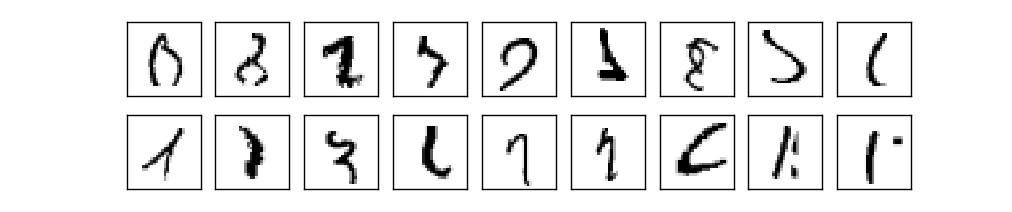
\includegraphics[width=0.933\textwidth]{images/mnist_really_bad_images.png}
\end{center}

\noindent 我相信你会同意这些图像很难分类！在 MNIST 数据集中有这样的图像的情况下，神经网络能够准确分类 10,000 幅测试图像中除 21 幅之外的所有图像，这是非常了不起的. 通常，在编程时我们认为解决像识别 MNIST 数字这样复杂的问题需要一个复杂的算法. 但即使是刚才提到的 Wan \emph{et al} 论文中的神经网络也只涉及相当简单的算法，即我们在本章中看到的算法的变体. 所有的复杂性都是从训练数据中自动学习到的. 在某种意义上，我们的结果和更复杂的论文中的结果所蕴含的寓意是，对于某些问题：复杂算法 $\leq$ 简单学习算法 + 好的训练数据.

\end{exerciseBox}
\sectionTitle{迈向深度学习}{迈向深度学习}

虽然我们的神经网络给出了令人印象深刻的表现，但这种表现多少有些神秘. 网络中的权重和偏置是自动发现的. 这意味着我们并不能立刻解释网络是如何做到它所做的事情的. 我们能否找到某种方式来理解我们的网络对手写数字进行分类所依据的原理？而且，如果有了这些原理，我们能否做得更好？

更直白地提出这些问题，假设几十年后神经网络带来了人工智能\label{term:45}（AI）. 我们会理解这些智能网络是如何工作的吗？也许这些网络对我们来说是不透明的，其中的权重和偏置我们并不理解，因为它们是自动学习出来的. 在人工智能研究的早期，人们希望构建人工智能的努力也能帮助我们理解智能背后的原理，也许还有人类大脑的运作方式. 但也许结果会是，我们最终既不理解大脑，也不理解人工智能是如何工作的！

为了回答这些问题，让我们回想一下我在本章开头给出的人工神经元的解释，即作为一种权衡证据的手段. 假设我们想确定一幅图像是否显示了一张人脸：\footnote{Credits: 1. Ester Inbar. 2. Unknown. 3. NASA, ESA, G. Illingworth, D. Magee, and P. Oesch (University of California, Santa Cruz), R. Bouwens (Leiden University), and the HUDF09 Team. Click on the images for more details.} 我们可以用处理手写数字识别的同样方式来攻克这个问题——把图像中的像素作为神经网络的输入，网络的输出是一个单独的神经元，表示``是的，这是一张脸''或``不，这不是一张脸''.

假设我们这样做，但我们不使用学习算法. 相反，我们要尝试手工设计一个网络，选择合适的权重和偏置. 我们该怎么做呢？暂时完全忘掉神经网络，我们可以使用的一个启发式方法是将问题分解为子问题：图像的左上方有眼睛吗？右上方有眼睛吗？中间有鼻子吗？下方中间有嘴巴吗？顶部有头发吗？等等.

如果其中几个问题的答案是``是''，或者甚至只是``可能是''，那么我们就会得出结论，这幅图像很可能是一张脸. 反过来，如果大多数问题的答案是``不''，那么这幅图像可能不是一张脸.

当然，这只是一个粗略的启发式方法，它有许多缺陷. 也许这个人是秃头，所以没有头发. 也许我们只能看到脸的一部分，或者脸是侧着的，所以一些面部特征被遮挡了. 尽管如此，这个启发式方法表明，如果我们能用神经网络解决这些子问题，那么也许我们可以通过组合这些子问题的网络来构建一个用于人脸检测的神经网络. 这里有一个可能的架构，矩形表示子网络. 注意，这并不是要作为解决人脸检测问题的现实方法；相反，它是为了帮助我们建立关于网络如何运作的直觉. 这是该架构：

\begin{center}
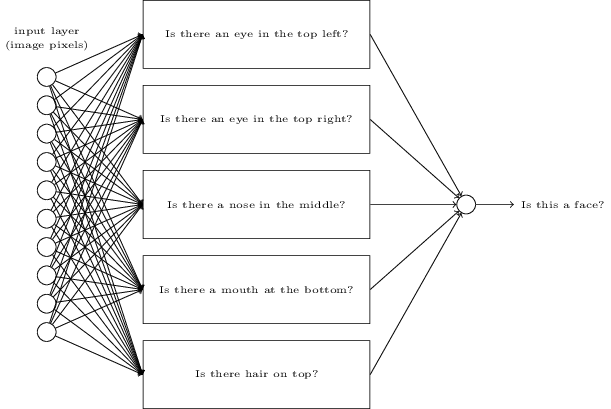
\includegraphics[width=0.9\textwidth]{images/tikz14.png}
\end{center}

\noindent 子网络也可以被分解，这也是合理的. 假设我们正在考虑这个问题：``左上方有眼睛吗？'' 这可以分解为诸如：``有眉毛吗？''；``有睫毛吗？''；``有虹膜吗？''；等等. 当然，这些问题实际上还应该包括位置信息——``眉毛在左上方，并且在虹膜上方吗？''，诸如此类——但让我们保持简单. 回答``左上方有眼睛吗？''这个问题的网络现在可以分解为：

\begin{center}
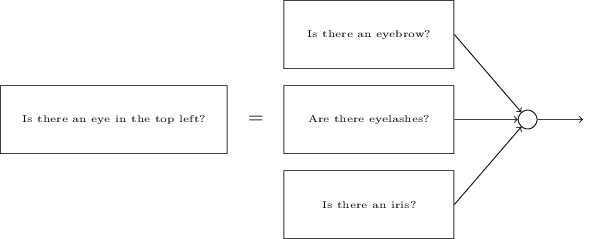
\includegraphics[width=0.9\textwidth]{images/tikz15.png}
\end{center}

\noindent 这些问题也可以被进一步分解，通过多个层越来越深入. 最终，我们将使用那些回答非常简单问题的子网络，这些问题简单到可以很容易地在单个像素的层面上回答. 例如，这些问题可能是关于图像中特定位置上是否存在非常简单的形状. 这样的问题可以由连接到图像中原始像素的单个神经元来回答.

最终结果是一个网络，它把一个非常复杂的问题——这幅图像是否显示了一张脸——分解为可以在单个像素层面上回答的非常简单的问题. 它通过一系列许多层来做到这一点，早期的层回答关于输入图像的非常简单和具体的问题，而后面的层则构建起一个越来越复杂和抽象的概念层次结构. 具有这种多层结构——两个或更多隐藏层——的网络被称为\emph{深度神经网络}.

当然，我还没有说明如何进行这种递归地分解为子网络. 手工设计网络中的权重和偏置当然是不切实际的. 相反，我们希望使用学习算法，使网络能够从训练数据中自动学习权重和偏置——从而学习概念的层次结构.20 世纪 80 年代和 90 年代的研究人员尝试使用随机梯度下降和反向传播来训练深度网络. 不幸的是，除了少数特殊架构外，他们并没有取得多大成功. 网络会学习，但非常缓慢，在实践中往往慢到没有用处.

自 2006 年以来，一系列技术被开发出来，使得在深度神经网络中进行学习成为可能. 这些深度学习技术基于随机梯度下降和反向传播，但也引入了新的思想. 这些技术使得训练更深（也更大）的网络成为可能——人们现在经常训练具有 5 到 10 个隐藏层的网络. 而且，事实证明，在许多问题上，这些网络的表现远远优于浅层神经网络，即只有一个隐藏层的网络. 原因当然是深度网络能够构建复杂的概念层次结构. 这有点像是传统编程语言使用模块化设计和抽象思想来创建复杂计算机程序的方式. 把深度网络与浅层网络进行比较，有点像是把一种能够进行函数调用的编程语言与一种被剥夺了这种调用能力的精简语言进行比较. 抽象在神经网络中采取的形式与传统编程中不同，但它同样重要.

\chapter{反向传播算法的工作原理}
在上一章中，我们看到了神经网络如何使用梯度下降算法来学习它们的权重和偏置. 然而，我们的解释中存在一个缺口：我们没有讨论如何计算代价函数的梯度. 这是一个相当大的缺口！在本章中，我将解释一种用于计算此类梯度的快速算法，这种算法被称为\emph{反向传播}（backpropagation）\label{term:46}.

反向传播算法\label{term:47}最初是在 20 世纪 70 年代引入的，但直到 1986 年 David Rumelhart、Geoffrey Hinton 和 Ronald Williams 发表了一篇著名论文之后，它的重要性才被充分认识到. 那篇论文描述了几种神经网络，其中反向传播的学习速度\label{term:48}远远快于早期的学习方法，使得用神经网络解决以前无法解决的问题成为可能. 如今，反向传播算法是神经网络学习的主力.

本章在数学上比本书其余部分更为复杂. 如果你对数学不太热衷，你可能会想跳过这一章，把反向传播当作一个黑箱\label{term:49}，愿意忽略其中的细节. 为什么要花时间去研究那些细节呢？

原因当然是理解. 反向传播的核心是一个表达式，它给出了代价函数 $C$ 关于网络中任意权重 $w$（或偏置 $b$）的偏导数 $\partial C / \partial w$. 这个表达式告诉我们，当我们改变权重和偏置时，代价变化得有多快. 虽然这个表达式有些复杂，但它也有一种美感，其中每个元素都有自然、直观的解释. 因此，反向传播不仅仅是一种快速的学习算法. 它实际上让我们深入了解到改变权重和偏置如何改变网络的整体行为. 这非常值得详细研究.

话虽如此，如果你想略读这一章，或者直接跳到下一章，那也没关系. 我把本书的其余部分写得即使你把反向传播当作黑箱也能理解. 当然，在本书后面的某些地方，我会回过头来引用本章的结果. 但在那些地方，即使你没有完全跟上所有推理，也应该仍然能够理解主要结论.
\sectionTitle{热身：基于矩阵的神经网络输出快速计算法}{热身：基于矩阵的神经网络输出快速计算法}

在讨论反向传播之前，让我们先用一个基于矩阵的快速算法来计算神经网络的输出，以此作为热身. 实际上我们在上一章末尾已经简要地看到过这个算法，但我当时讲得很快，所以值得详细地重新审视. 特别是，这是在熟悉的语境中熟悉反向传播所用记号的好方法.

让我们从一个记号开始，它让我们能够以明确无歧义的方式引用网络中的权重. 我们将用 $w^l_{jk}$ 表示从第 $(l-1)$ 层的第 $k$ 个神经元到第 $l$ 层的第 $j$ 个神经元的连接权重. 例如，下图显示了网络中从第二层的第四个神经元到第三层的第二个神经元的连接上的权重：

\begin{center}
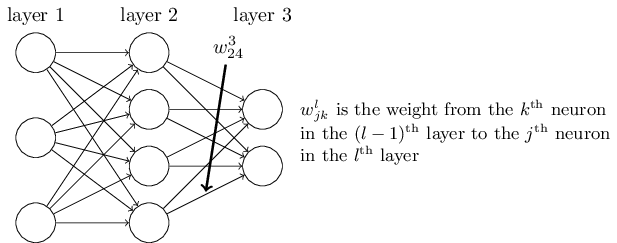
\includegraphics[width=0.9\textwidth]{images/tikz16.png}
\end{center}

\noindent 这个记号起初很笨拙，确实需要花些功夫才能掌握. 但只要稍加努力，你就会发现这个记号变得简单而自然. 这个记号的一个古怪之处是 $j$ 和 $k$ 下标的顺序. 你可能会认为用 $j$ 指代输入神经元、用 $k$ 指代输出神经元更合理，而不是像实际所做的那样反过来. 我将在下面解释这个古怪之处的原因.

我们对网络的偏置和激活值使用类似的记号. 具体来说，我们用 $b^l_j$ 表示第 $l$ 层第 $j$ 个神经元的偏置. 我们用 $a^l_j$ 表示第 $l$ 层第 $j$ 个神经元的激活值. 下图展示了这些记号的使用示例：

\begin{center}
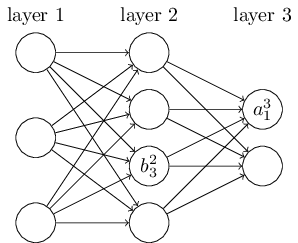
\includegraphics[width=0.9\textwidth]{images/tikz17.png}
\end{center}

\noindent 有了这些记号，第 $l$ 层第 $j$ 个神经元的激活值 $a^{l}_j$ 与第 $(l-1)$ 层的激活值通过以下方程相关联（比较上一章中的方程 (4)

\begin{align*}
\frac{1}{1+\exp(-\sum_j w_j x_j-b)} \nonumber
\end{align*}

\noindent 及周围的讨论）

\begin{equation}
a^{l}_j = \sigma\left( \sum_k w^{l}_{jk} a^{l-1}_k + b^l_j \right),
\tag{23}
\end{equation}

\noindent 其中求和是对第 $(l-1)$ 层中的所有神经元 $k$ 进行的. 为了将这个表达式改写为矩阵形式，我们为每一层 $l$ 定义一个权重矩阵 $w^l$. 权重矩阵 $w^l$ 的元素就是连接到第 $l$ 层神经元的权重，也就是说，第 $j$ 行第 $k$ 列的元素是 $w^l_{jk}$. 类似地，对于每一层 $l$，我们定义一个偏置向量 $b^l$. 你大概能猜到这是如何运作的——偏置向量的分量就是值 $b^l_j$，第 $l$ 层中的每个神经元对应一个分量. 最后，我们定义一个激活向量 $a^l$，其分量是激活值 $a^l_j$.

将 (23)

\begin{align*}
a^{l}_j = \sigma\left( \sum_k w^{l}_{jk} a^{l-1}_k + b^l_j \right) \nonumber
\end{align*}

\noindent 改写为矩阵形式所需的最后一个要素是函数向量化的概念，例如 $\sigma$. 我们在上一章简要接触过向量化，但回顾一下，其思想是我们想要将一个函数（如 $\sigma$）应用于向量 $v$ 中的每一个元素. 我们用显而易见的记号 $\sigma(v)$ 来表示这种逐元素应用函数的方式. 也就是说，$\sigma(v)$ 的分量就是 $\sigma(v)_j = \sigma(v_j)$. 举个例子，如果我们有函数 $f(x) = x^2$，那么 $f$ 的向量化形式的效果是

\begin{equation}
f\left(\left[ \begin{array}{c} 2 \\ 3 \end{array} \right] \right) = \left[ \begin{array}{c} f(2) \\ f(3) \end{array} \right] = \left[ \begin{array}{c} 4 \\ 9 \end{array} \right],
\tag{24}
\end{equation}

\noindent 也就是说，向量化的 $f$ 只是对向量的每个元素求平方.

有了这些记号，方程 (23)

\begin{align*}
a^{l}_j = \sigma\left( \sum_k w^{l}_{jk} a^{l-1}_k + b^l_j \right) \nonumber
\end{align*}

\noindent 可以改写为优美而紧凑的向量化形式

\begin{equation}
a^{l} = \sigma(w^l a^{l-1}+b^l).
\tag{25}
\end{equation}

\noindent 这个表达式为我们提供了一种更加全局的方式来思考一层中的激活值与上一层激活值之间的关系：我们只需将权重矩阵应用于激活值，然后加上偏置向量，最后应用 $\sigma$ 函数*\footnote{顺便说一下，正是这个表达式促成了前面提到的 $w^l_{jk}$ 记号中的古怪之处. 如果我们用 $j$ 来索引输入神经元、用 $k$ 来索引输出神经元，那么我们就需要将方程 (25)$a^{l} = \sigma(w^l a^{l-1}+b^l)$ 中的权重矩阵替换为其转置. 这是一个小改动，但很烦人，而且我们会失去说（和思考）``将权重矩阵应用于激活值''的那种简单明了.}. 这种全局视角通常比我们到目前为止所采用的逐个神经元的视角更容易、更简洁（而且涉及的指标更少！）. 可以把它看作一种摆脱指标地狱的方式，同时对正在发生的事情保持精确. 这个表达式在实践中也很有用，因为大多数矩阵库都提供了实现矩阵乘法、向量加法和向量化的快速方法. 事实上，上一章中的代码就隐含地使用了这个表达式来计算网络的行为.

当使用方程 (25)

\begin{align*}
a^{l} = \sigma(w^l a^{l-1}+b^l) \nonumber
\end{align*}

\noindent 来计算 $a^l$ 时，我们会在此过程中计算中间量 $z^l \equiv w^l a^{l-1}+b^l$. 这个量足够有用，值得给它起个名字：我们称 $z^l$ 为第 $l$ 层神经元的\emph{加权输入}. 我们将在本章后面大量使用加权输入 $z^l$. 方程 (25)

\begin{align*}
a^{l} = \sigma(w^l a^{l-1}+b^l) \nonumber
\end{align*}

\noindent 有时用加权输入来写，即 $a^l = \sigma(z^l)$. 还值得注意的是，$z^l$ 的分量为 $z^l_j = \sum_k w^l_{jk} a^{l-1}_k+b^l_j$，也就是说，$z^l_j$ 就是第 $l$ 层中神经元 $j$ 的激活函数的加权输入.
\sectionTitle{我们需要对代价函数做出的两条假设}{我们需要对代价函数做出的两条假设}

反向传播的目标是计算代价函数 $C$ 关于网络中任意权重 $w$ 或偏置 $b$ 的偏导数 $\partial C / \partial w$ 和 $\partial C / \partial b$. 为了让反向传播能够工作，我们需要对代价函数的形式做出两条主要假设. 不过在陈述这些假设之前，先在心里有一个代价函数的例子会很有帮助. 我们将使用上一章中的二次代价函数（参见公式 (6)

\begin{align*}
C(w,b) \equiv \frac{1}{2n} \sum_x \| y(x) - a\|^2 \nonumber
\end{align*}

\noindent ）. 用上一节的记号，二次代价具有如下形式

\begin{equation}
C = \frac{1}{2n} \sum_x \|y(x)-a^L(x)\|^2,
\tag{26}
\end{equation}

\noindent 其中：$n$ 是训练样本的总数；求和是对各个训练样本 $x$ 进行的；$y = y(x)$ 是相应的期望输出；$L$ 表示网络中的层数；而 $a^L = a^L(x)$ 是当输入为 $x$ 时网络输出的激活值向量.

好，那么为了让反向传播能够应用，我们需要对代价函数 $C$ 做出什么假设呢？我们需要的第一条假设是，代价函数可以写成对各个训练样本 $x$ 的代价函数 $C_x$ 求平均的形式 $C = \frac{1}{n} \sum_x C_x$. 二次代价函数就属于这种情况，其中单个训练样本的代价为 $C_x = \frac{1}{2} \|y-a^L \|^2$. 这条假设对于本书中我们将遇到的所有其他代价函数也同样成立.

我们需要这条假设的原因是，反向传播实际上让我们做的是计算单个训练样本的偏导数 $\partial C_x / \partial w$ 和 $\partial C_x / \partial b$. 然后我们通过对训练样本求平均来恢复 $\partial C / \partial w$ 和 $\partial C / \partial b$. 事实上，有了这条假设，我们将假定训练样本 $x$ 已经固定，并去掉 $x$ 下标，把代价 $C_x$ 写成 $C$. 我们最终会把 $x$ 放回去，但就目前而言，这是一个最好隐去不写的记号上的麻烦.

我们对代价做出的第二条假设是，它可以写成神经网络输出的函数：

\begin{center}
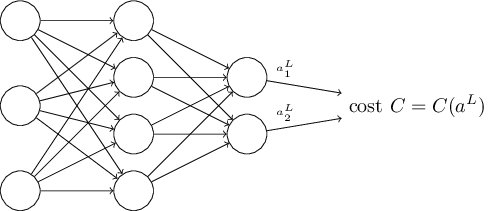
\includegraphics[width=0.9\textwidth]{images/tikz18.png}
\end{center}

\noindent 例如，二次代价函数满足这一要求，因为单个训练样本 $x$ 的二次代价可以写成

\begin{equation}
C = \frac{1}{2} \|y-a^L\|^2 = \frac{1}{2} \sum_j (y_j-a^L_j)^2,
\tag{27}
\end{equation}

\noindent 因此它是输出激活值的函数. 当然，这个代价函数也依赖于期望输出 $y$，你可能会奇怪为什么我们不把代价也看作 $y$ 的函数. 不过请记住，输入训练样本 $x$ 是固定的，因此输出 $y$ 也是一个固定的参数. 特别地，它不是我们能够通过以任何方式改变权重和偏置来修改的东西，也就是说，它不是神经网络所学习的东西. 因此，把 $C$ 看作仅依赖于输出激活值 $a^L$ 的函数是合理的，而 $y$ 仅仅是帮助定义该函数的一个参数.
\sectionTitle{Hadamard 积，$s \odot t$}{Hadamard 积，$s \odot t$}

反向传播算法基于常见的线性代数运算——比如向量加法、向量与矩阵相乘等等. 但其中有一种运算不太常用. 具体来说，假设 $s$ 和 $t$ 是两个维度相同的向量. 那么我们使用 $s \odot t$ 来表示这两个向量的\emph{逐元素}乘积. 因此 $s \odot t$ 的分量就是 $(s \odot t)_j = s_j t_j$. 举个例子，

\begin{equation}
\left[\begin{array}{c} 1 \\ 2 \end{array}\right] \odot \left[\begin{array}{c} 3 \\ 4\end{array} \right] = \left[ \begin{array}{c} 1 * 3 \\ 2 * 4 \end{array} \right] = \left[ \begin{array}{c} 3 \\ 8 \end{array} \right].
\tag{28}
\end{equation}

\noindent 这种逐元素乘法有时被称为 \emph{Hadamard 积}或 \emph{Schur 积}. 我们将称之为 Hadamard 积. 优秀的矩阵库通常会提供 Hadamard 积的快速实现，这在实现反向传播时非常方便.
\sectionTitle{反向传播背后的四个基本方程}{反向传播背后的四个基本方程}

反向传播关乎理解网络中权重和偏置的改变如何改变代价函数. 归根结底，这意味着计算偏导数 $\partial C / \partial w^l_{jk}$ 和 $\partial C / \partial b^l_j$. 但为了计算这些，我们首先引入一个中间量 $\delta^l_j$，我们称之为第 $l$ 层第 $j$ 个神经元的\emph{误差}. 反向传播将为我们提供一个计算误差 $\delta^l_j$ 的过程，然后将 $\delta^l_j$ 与 $\partial C / \partial w^l_{jk}$ 和 $\partial C / \partial b^l_j$ 联系起来.

为了理解误差是如何定义的，想象在我们的神经网络中有一个恶魔：

\begin{center}
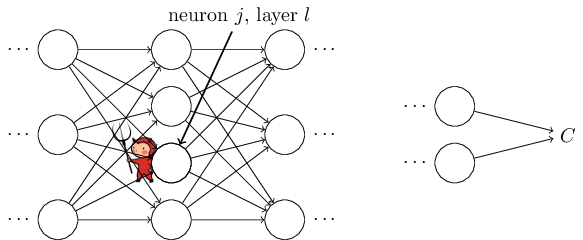
\includegraphics[width=0.9\textwidth]{images/tikz19.png}
\end{center}

\noindent 这个恶魔坐在第 $l$ 层的第 $j$ 个神经元处. 当神经元的输入到来时，恶魔干扰了神经元的运算. 它给神经元的加权输入加上一点变化 $\Delta z^l_j$，使得神经元不是输出 $\sigma(z^l_j)$，而是输出 $\sigma(z^l_j+\Delta z^l_j)$. 这个变化通过网络中后面的层传播，最终导致整体代价改变 $\frac{\partial C}{\partial z^l_j} \Delta z^l_j$.

现在，这个恶魔是一个好恶魔，它试图帮助你改善代价，也就是说，它试图找到一个使代价变小的 $\Delta z^l_j$. 假设 $\frac{\partial C}{\partial z^l_j}$ 有一个很大的值（无论是正还是负）. 那么恶魔可以通过选择 $\Delta z^l_j$ 与 $\frac{\partial C}{\partial z^l_j}$ 符号相反来大幅降低代价. 相比之下，如果 $\frac{\partial C}{\partial z^l_j}$ 接近于零，那么恶魔通过扰动加权输入 $z^l_j$ 根本无法大幅改善代价. 就恶魔所能判断的而言，这个神经元已经非常接近最优了*\footnote{当然，这只对小的变化 $\Delta z^l_j$ 成立. 我们将假设恶魔被限制只能做这样小的变化.}. 因此，从启发式的意义上说， $\frac{\partial C}{\partial z^l_j}$ 是神经元误差的一种度量.

受这个故事的启发，我们定义第 $l$ 层神经元 $j$ 的误差 $\delta^l_j$ 为

\begin{equation}
\delta^l_j \equiv \frac{\partial C}{\partial z^l_j}.
\tag{29}
\end{equation}

\noindent 按照我们通常的约定，我们用 $\delta^l$ 表示与第 $l$ 层相关的误差向量. 反向传播将为我们提供一种计算每一层的 $\delta^l$ 的方法，然后将这些误差与真正感兴趣的量为 $\partial C / \partial w^l_{jk}$ 和 $\partial C / \partial b^l_j$ 联系起来.

你可能想知道为什么恶魔改变的是加权输入 $z^l_j$. 当然，想象恶魔改变输出激活值 $a^l_j$ 会更自然，这样我们就会用 $\frac{\partial C}{\partial a^l_j}$ 作为误差的度量. 事实上，如果你这样做，结果与下面的讨论非常相似. 但事实证明，这会使反向传播的表述在代数上稍微复杂一些. 所以我们坚持用 $\delta^l_j = \frac{\partial C}{\partial z^l_j}$ 作为误差的度量*\footnote{在像 MNIST 这样的分类问题中， ``误差''一词有时被用来表示分类失败率. 例如，如果神经网络正确分类了 96.0\% 的数字，那么误差就是 4.0\%. 显然，这与我们的 $\delta$ 向量有着完全不同的含义. 在实践中，你应该不难判断在任何给定的用法中指的是哪种含义.}. \textbf{进攻计划：} 反向传播基于四个基本方程. 这些方程共同为我们提供了一种计算误差 $\delta^l$ 和代价函数梯度的方法. 我在下面陈述这四个方程. 但请注意：你不应该期望能瞬间消化这些方程. 这样的期望会导致失望. 事实上，反向传播方程如此丰富，以至于要很好地理解它们需要相当的时间和耐心，随着你逐渐深入这些方程. 好消息是，这样的耐心会得到许多倍的回报. 因此，本节的讨论仅仅是一个开始，帮助你在彻底理解这些方程的道路上前进.

以下是我们在本章后面更深入地探讨这些方程的方式预览：我将给出方程的简短证明，这有助于解释它们为什么是正确的；我们将以伪代码的算法形式重述这些方程，并看看伪代码如何实现为真正运行的 Python 代码；并且，在本章最后一节中，我们将发展一个关于反向传播方程含义的直观图景，以及某人如何可能从零开始发现它们. 在此过程中，我们将反复回到这四个基本方程，随着你理解的加深，这些方程将变得舒适，也许甚至美丽而自然. \textbf{输出层误差 $\delta^L$ 的方程：} $\delta^L$ 的分量由下式给出

\begin{equation}
\delta^L_j = \frac{\partial C}{\partial a^L_j} \sigma'(z^L_j).
\tag{BP1}
\end{equation}

\noindent 这是一个非常自然的表达式. 右边的第一项 $\partial C / \partial a^L_j$ 只是衡量代价作为第 $j$ 个输出激活值的函数变化有多快. 例如，如果 $C$ 不太依赖于某个特定的输出神经元 $j$，那么 $\delta^L_j$ 就会很小，这正是我们所期望的. 右边的第二项 $\sigma'(z^L_j)$ 衡量激活函数 $\sigma$ 在 $z^L_j$ 处变化有多快.

注意 (BP1) 中的所有内容

\begin{align*}
\delta^L_j = \frac{\partial C}{\partial a^L_j} \sigma'(z^L_j) \nonumber
\end{align*}

\noindent 都很容易计算. 特别地，我们在计算网络行为时计算 $z^L_j$，而计算 $\sigma'(z^L_j)$ 只需要很小的额外开销. $\partial C / \partial a^L_j$ 的确切形式当然取决于代价函数的形式. 然而，只要代价函数已知，计算 $\partial C / \partial a^L_j$ 应该没有什么困难. 例如，如果我们使用二次代价函数，那么 $C = \frac{1}{2} \sum_j (y_j-a^L_j)^2$，因此 $\partial C / \partial a^L_j = (a_j^L-y_j)$，这显然很容易计算.

方程 (BP1)

\begin{align*}
\delta^L_j = \frac{\partial C}{\partial a^L_j} \sigma'(z^L_j) \nonumber
\end{align*}

\noindent 是 $\delta^L$ 的逐分量表达式. 这是一个非常好的表达式，但不是我们为反向传播想要的基于矩阵的形式. 然而，很容易将方程重写为基于矩阵的形式，即

\begin{equation}
\delta^L = \nabla_a C \odot \sigma'(z^L).
\tag{BP1a}
\end{equation}

\noindent 这里， $\nabla_a C$ 被定义为一个向量，其分量为偏导数 $\partial C / \partial a^L_j$. 你可以把 $\nabla_a C$ 看作表达 $C$ 相对于输出激活值的变化率. 很容易看出方程 (BP1a)

\begin{align*}
\delta^L = \nabla_a C \odot \sigma'(z^L) \nonumber
\end{align*}

\noindent 和 (BP1)

\begin{align*}
\delta^L_j = \frac{\partial C}{\partial a^L_j} \sigma'(z^L_j) \nonumber
\end{align*}

\noindent 是等价的，因此从现在起我们将互换使用 (BP1)

\begin{align*}
\delta^L_j = \frac{\partial C}{\partial a^L_j} \sigma'(z^L_j) \nonumber
\end{align*}

\noindent 来指代这两个方程. 作为一个例子，在二次代价的情况下，我们有 $\nabla_a C = (a^L-y)$，因此 (BP1) 的完全基于矩阵的形式

\begin{align*}
\delta^L_j = \frac{\partial C}{\partial a^L_j} \sigma'(z^L_j) \nonumber
\end{align*}

\noindent 变为

\begin{equation}
\delta^L = (a^L-y) \odot \sigma'(z^L).
\tag{30}
\end{equation}

\noindent 如你所见，这个表达式中的所有内容都有很好的向量形式，并且很容易使用像 Numpy 这样的库来计算. \textbf{用下一层误差 $\delta^{l+1}$ 表示误差 $\delta^l$ 的方程：} 特别地

\begin{equation}
\delta^l = ((w^{l+1})^T \delta^{l+1}) \odot \sigma'(z^l),
\tag{BP2}
\end{equation}

\noindent 其中 $(w^{l+1})^T$ 是第 $(l+1)$ 层权重矩阵 $w^{l+1}$ 的转置. 这个方程看起来很复杂，但每个元素都有很好的解释. 假设我们知道第 $l+1$ 层的误差 $\delta^{l+1}$. 当我们应用转置权重矩阵 $(w^{l+1})^T$ 时，我们可以直观地认为这是将误差通过网络\emph{反向}移动，给我们某种第 $l$ 层输出处误差的度量. 然后我们取 Hadamard 积 $\odot \sigma'(z^l)$. 这将误差通过第 $l$ 层的激活函数反向移动，给出第 $l$ 层加权输入中的误差 $\delta^l$.

通过将 (BP2)

\begin{align*}
\delta^l = ((w^{l+1})^T \delta^{l+1}) \odot \sigma'(z^l) \nonumber
\end{align*}

\noindent 与 (BP1)

\begin{align*}
\delta^L_j = \frac{\partial C}{\partial a^L_j} \sigma'(z^L_j) \nonumber
\end{align*}

\noindent 结合，我们可以计算网络中任意层的误差 $\delta^l$. 我们首先使用 (BP1)

\begin{align*}
\delta^L_j = \frac{\partial C}{\partial a^L_j} \sigma'(z^L_j) \nonumber
\end{align*}

\noindent 计算 $\delta^L$，然后应用方程 (BP2)

\begin{align*}
\delta^l = ((w^{l+1})^T \delta^{l+1}) \odot \sigma'(z^l) \nonumber
\end{align*}

\noindent 计算 $\delta^{L-1}$，然后再次应用方程 (BP2)

\begin{align*}
\delta^l = ((w^{l+1})^T \delta^{l+1}) \odot \sigma'(z^l) \nonumber
\end{align*}

\noindent 计算 $\delta^{L-2}$，依此类推，一直反向通过网络. \textbf{代价相对于网络中任意偏置的变化率的方程：} 特别地：

\begin{equation}
\frac{\partial C}{\partial b^l_j} = \delta^l_j.
\tag{BP3}
\end{equation}

\noindent 也就是说，误差 $\delta^l_j$ \emph{恰好等于}变化率 $\partial C / \partial b^l_j$. 这是个好消息，因为 (BP1)

\begin{align*}
\delta^L_j = \frac{\partial C}{\partial a^L_j} \sigma'(z^L_j) \nonumber
\end{align*}

\noindent 和 (BP2)

\begin{align*}
\delta^l = ((w^{l+1})^T \delta^{l+1}) \odot \sigma'(z^l) \nonumber
\end{align*}

\noindent 已经告诉我们如何计算 $\delta^l_j$. 我们可以将 (BP3)

\begin{align*}
\frac{\partial C}{\partial b^l_j} = \delta^l_j \nonumber
\end{align*}

\noindent 简写为

\begin{equation}
\frac{\partial C}{\partial b} = \delta,
\tag{31}
\end{equation}

\noindent 其中 $\delta$ 被理解为在与偏置 $b$ 相同的神经元处求值. \textbf{代价相对于网络中任意权重的变化率的方程：} 特别地：

\begin{equation}
\frac{\partial C}{\partial w^l_{jk}} = a^{l-1}_k \delta^l_j.
\tag{BP4}
\end{equation}
\noindent 这告诉我们如何用已经知道如何计算的量 $\delta^l$ 和 $a^{l-1}$ 来计算偏导数 $\partial C / \partial w^l_{jk}$. 这个方程可以用一种下标更少的记号重写为

\begin{equation}
\frac{\partial C}{\partial w} = a_{\rm in} \delta_{\rm out},
\tag{32}
\end{equation}

\noindent 其中我们约定 $a_{\rm in}$ 是输入到权重 $w$ 的神经元的激活值，而 $\delta_{\rm out}$ 是从权重 $w$ 输出的神经元的误差. 放大来看，只关注权重 $w$ 以及由该权重连接的两个神经元，我们可以将其描绘为：

\begin{center}
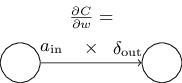
\includegraphics[width=0.9\textwidth]{images/tikz20.png}
\end{center}

\noindent 方程 (32)

\begin{align*}
\frac{\partial C}{\partial w} = a_{\rm in} \delta_{\rm out} \nonumber
\end{align*}

\noindent 的一个很好的推论是，当激活值 $a_{\rm in}$ 很小时，$a_{\rm in} \approx 0$，梯度项 $\partial C / \partial w$ 也会趋于很小. 在这种情况下，我们说该权重学习缓慢，意思是它在梯度下降过程中变化不大. 换句话说，(BP4)

\begin{align*}
\frac{\partial C}{\partial w^l_{jk}} = a^{l-1}_k \delta^l_j \nonumber
\end{align*}

\noindent 的一个推论是，从低激活值神经元输出的权重学习缓慢.

沿着这些思路，还可以从 (BP1)

\begin{align*}
\delta^L_j = \frac{\partial C}{\partial a^L_j} \sigma'(z^L_j) \nonumber
\end{align*}

\noindent -(BP4)

\begin{align*}
\frac{\partial C}{\partial w^l_{jk}} = a^{l-1}_k \delta^l_j \nonumber
\end{align*}

\noindent 中得到其他洞见. 让我们先看输出层. 考虑 (BP1)

\begin{align*}
\delta^L_j = \frac{\partial C}{\partial a^L_j} \sigma'(z^L_j) \nonumber
\end{align*}

\noindent 中的项 $\sigma'(z^L_j)$. 回想上一章中 sigmoid 函数的图像，当 $\sigma(z^L_j)$ 近似为 $0$ 或 $1$ 时，$\sigma$ 函数会变得非常平坦. 当这种情况发生时，我们将有 $\sigma'(z^L_j) \approx 0$. 因此，教训是：如果输出神经元处于低激活值（$\approx 0$）或高激活值（$\approx 1$），最后一层的权重将学习缓慢. 在这种情况下，通常说该输出神经元已经 \emph{饱和}，因此该权重已经停止学习（或学习缓慢）. 类似的评论也适用于输出神经元的偏置.

对于更早的层，我们可以得到类似的洞见. 特别地，注意 (BP2)

\begin{align*}
\delta^l = ((w^{l+1})^T \delta^{l+1}) \odot \sigma'(z^l) \nonumber
\end{align*}

\noindent 中的 $\sigma'(z^l)$ 项. 这意味着如果神经元接近饱和，$\delta^l_j$ 很可能变得很小. 而这又意味着，输入到饱和神经元的任何权重都将学习缓慢*\footnote{如果 ${w^{l+1}}^T \delta^{l+1}$ 的元素足够大，足以补偿 $\sigma'(z^l_j)$ 的微小，这个推理就不成立. 但我说的是一般趋势.}.

总结一下，我们已经了解到，如果输入神经元处于低激活值，或者输出神经元已经饱和，即处于高激活值或低激活值，那么权重将学习缓慢.

这些观察都不太令人惊讶. 不过，它们有助于改进我们对神经网络学习过程中所发生事情的心智模型. 此外，我们可以反过来利用这类推理. 这四个基本方程对任何激活函数都成立，而不仅仅是标准的 sigmoid 函数（这是因为，正如我们稍后将看到的，证明没有使用 $\sigma$ 的任何特殊性质）. 因此我们可以用这些方程来 \emph{设计} 具有特定所需学习性质的激活函数. 作为给你一个思路的例子，假设我们选择一个（非 sigmoid）激活函数 $\sigma$，使得 $\sigma'$ 始终为正，且永远不会接近零. 那将防止普通 sigmoid 神经元饱和时出现的学习减慢. 在本书后面，我们将看到对激活函数进行这种修改的例子. 牢记这四个方程 (BP1)

\begin{align*}
\delta^L_j = \frac{\partial C}{\partial a^L_j} \sigma'(z^L_j) \nonumber
\end{align*}

\noindent -(BP4)

\begin{align*}
\frac{\partial C}{\partial w^l_{jk}} = a^{l-1}_k \delta^l_j \nonumber
\end{align*}

\noindent 有助于解释为什么尝试这样的修改，以及它们可能产生什么影响.

\begin{center}
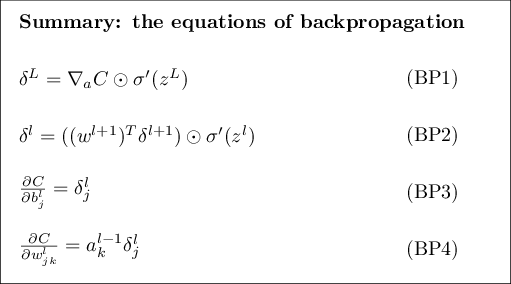
\includegraphics[width=0.9\textwidth]{images/tikz21.png}
\end{center}

\begin{exerciseBox}{习题}

\begin{itemize}

\item
\textbf{反向传播方程的另一种表述：} 我用 Hadamard 积陈述了反向传播的方程（特别是 (BP1)

\begin{align*}
\delta^L_j = \frac{\partial C}{\partial a^L_j} \sigma'(z^L_j) \nonumber
\end{align*}

和 (BP2)

\begin{align*}
\delta^l = ((w^{l+1})^T \delta^{l+1}) \odot \sigma'(z^l) \nonumber
\end{align*}

）. 如果你不熟悉 Hadamard 积，这种表述可能会让你感到困惑. 还有一种基于传统矩阵乘法的替代方法，一些读者可能会觉得有启发性. (1) 证明 (BP1)

\begin{align*}
\delta^L_j = \frac{\partial C}{\partial a^L_j} \sigma'(z^L_j) \nonumber
\end{align*}

可以重写为

\begin{equation}
\delta^L = \Sigma'(z^L) \nabla_a C,
\tag{33}
\end{equation}

其中 $\Sigma'(z^L)$ 是一个方阵，其对角元素是值 $\sigma'(z^L_j)$，非对角元素为零. 注意这个矩阵通过传统矩阵乘法作用于 $\nabla_a C$. (2) 证明 (BP2)

\begin{align*}
\delta^l = ((w^{l+1})^T \delta^{l+1}) \odot \sigma'(z^l) \nonumber
\end{align*}

可以重写为

\begin{equation}
\delta^l = \Sigma'(z^l) (w^{l+1})^T \delta^{l+1}.
\tag{34}
\end{equation}

(3) 结合观察 (1) 和 (2)，证明

\begin{equation}
\delta^l = \Sigma'(z^l) (w^{l+1})^T \ldots \Sigma'(z^{L-1}) (w^L)^T \Sigma'(z^L) \nabla_a C
\tag{35}
\end{equation}

对于熟悉矩阵乘法的读者，这个方程可能比 (BP1)

\begin{align*}
\delta^L_j = \frac{\partial C}{\partial a^L_j} \sigma'(z^L_j) \nonumber
\end{align*}

和 (BP2)

\begin{align*}
\delta^l = ((w^{l+1})^T \delta^{l+1}) \odot \sigma'(z^l) \nonumber
\end{align*}

更容易理解. 我之所以关注 (BP1)

\begin{align*}
\delta^L_j = \frac{\partial C}{\partial a^L_j} \sigma'(z^L_j) \nonumber
\end{align*}

和 (BP2)

\begin{align*}
\delta^l = ((w^{l+1})^T \delta^{l+1}) \odot \sigma'(z^l) \nonumber
\end{align*}

，是因为那种方法在数值实现上更快.

\end{itemize}

\end{exerciseBox}
\sectionTitle{四个基本方程的证明（选读）}{四个基本方程的证明（选读）}

我们现在来证明四个基本方程 (BP1)

\begin{align*}
\delta^L_j = \frac{\partial C}{\partial a^L_j} \sigma'(z^L_j) \nonumber
\end{align*}

\noindent -(BP4)

\begin{align*}
\frac{\partial C}{\partial w^l_{jk}} = a^{l-1}_k \delta^l_j \nonumber
\end{align*}

\noindent. 这四个方程都是多元微积分中链式法则的结果. 如果你对链式法则比较熟悉，那么我强烈建议你在继续阅读之前先自己尝试推导一遍.

我们从方程 (BP1)

\begin{align*}
\delta^L_j = \frac{\partial C}{\partial a^L_j} \sigma'(z^L_j) \nonumber
\end{align*}

\noindent 开始，它给出了输出误差 $\delta^L$ 的表达式. 为了证明这个方程，回忆一下根据定义

\begin{equation}
\delta^L_j = \frac{\partial C}{\partial z^L_j}.
\tag{36}
\end{equation}

\noindent 应用链式法则，我们可以将上面的偏导数重新表达为关于输出激活值的偏导数，

\begin{equation}
\delta^L_j = \sum_k \frac{\partial C}{\partial a^L_k} \frac{\partial a^L_k}{\partial z^L_j},
\tag{37}
\end{equation}

\noindent 其中求和是对输出层中所有神经元 $k$ 进行的. 当然，当 $k = j$ 时，第 $k$ 个神经元的输出激活值 $a^L_k$ 只依赖于第 $j$ 个神经元的加权输入 $z^L_j$. 因此当 $k \neq j$ 时 $\partial a^L_k / \partial z^L_j$ 为零. 于是我们可以将前面的方程简化为

\begin{equation}
\delta^L_j = \frac{\partial C}{\partial a^L_j} \frac{\partial a^L_j}{\partial z^L_j}.
\tag{38}
\end{equation}

\noindent 回忆 $a^L_j = \sigma(z^L_j)$，右边的第二项可以写成 $\sigma'(z^L_j)$，方程变为

\begin{equation}
\delta^L_j = \frac{\partial C}{\partial a^L_j} \sigma'(z^L_j),
\tag{39}
\end{equation}

\noindent 这正是 (BP1)

\begin{align*}
\delta^L_j = \frac{\partial C}{\partial a^L_j} \sigma'(z^L_j) \nonumber
\end{align*}

\noindent 的分量形式.

接下来，我们将证明 (BP2)

\begin{align*}
\delta^l = ((w^{l+1})^T \delta^{l+1}) \odot \sigma'(z^l) \nonumber
\end{align*}

\noindent，它给出了误差 $\delta^l$ 与下一层误差 $\delta^{l+1}$ 之间的关系式. 为此，我们希望将 $\delta^l_j = \partial C / \partial z^l_j$ 用 $\delta^{l+1}_k = \partial C / \partial z^{l+1}_k$ 重新表达. 我们可以利用链式法则做到这一点，

\begin{align}
\delta^l_j &= \frac{\partial C}{\partial z^l_j} \tag{40} \\ &= \sum_k \frac{\partial C}{\partial z^{l+1}_k} \frac{\partial z^{l+1}_k}{\partial z^l_j} \tag{41} \\ &= \sum_k \frac{\partial z^{l+1}_k}{\partial z^l_j} \delta^{l+1}_k, \tag{42}
\end{align}

\noindent 在最后一行中我们交换了右边的两项，并代入了 $\delta^{l+1}_k$ 的定义. 为了计算最后一行的第一项，注意到

\begin{equation}
z^{l+1}_k = \sum_j w^{l+1}_{kj} a^l_j +b^{l+1}_k = \sum_j w^{l+1}_{kj} \sigma(z^l_j) +b^{l+1}_k.
\tag{43}
\end{equation}

\noindent 求导，我们得到

\begin{equation}
\frac{\partial z^{l+1}_k}{\partial z^l_j} = w^{l+1}_{kj} \sigma'(z^l_j).
\tag{44}
\end{equation}

\noindent 代回 (42)

\begin{align*}
&= \sum_k \frac{\partial z^{l+1}_k}{\partial z^l_j} \delta^{l+1}_k \nonumber
\end{align*}

\noindent 我们得到

\begin{equation}
\delta^l_j = \sum_k w^{l+1}_{kj} \delta^{l+1}_k \sigma'(z^l_j).
\tag{45}
\end{equation}

\noindent 这正是 (BP2)

\begin{align*}
\delta^l = ((w^{l+1})^T \delta^{l+1}) \odot \sigma'(z^l) \nonumber
\end{align*}

\noindent 的分量形式.

我们要证明的最后两个方程是 (BP3)

\begin{align*}
\frac{\partial C}{\partial b^l_j} = \delta^l_j \nonumber
\end{align*}

\noindent 和 (BP4)

\begin{align*}
\frac{\partial C}{\partial w^l_{jk}} = a^{l-1}_k \delta^l_j \nonumber
\end{align*}

\noindent. 它们同样可以由链式法则推出，方式与上面两个方程的证明类似. 我把它们留给你作为练习.

\begin{exerciseBox}{练习}

\begin{itemize}

\item
证明方程 (BP3)

\begin{align*}
\frac{\partial C}{\partial b^l_j} = \delta^l_j \nonumber
\end{align*}

和 (BP4)

\begin{align*}
\frac{\partial C}{\partial w^l_{jk}} = a^{l-1}_k \delta^l_j \nonumber
\end{align*}

.

\end{itemize}

这就完成了反向传播四个基本方程的证明. 证明看起来可能很复杂. 但它实际上只是仔细应用链式法则的结果. 更简洁地说，我们可以把反向传播看作一种通过系统地应用多元微积分中的链式法则来计算代价函数梯度的方法. 反向传播本质上就是这些——其余的都是细节.

\end{exerciseBox}
\sectionTitle{反向传播算法}{反向传播算法}

反向传播方程为我们提供了一种计算代价函数梯度的方法. 让我们以算法的形式明确地写出来：

\begin{enumerate}

\item \textbf{输入 $x$：} 为输入层设置对应的激活值 $a^{1}$.

\item \textbf{前馈：} 对每个 $l = 2, 3, \ldots, L$ 计算 $z^{l} = w^l a^{l-1}+b^l$ 和 $a^{l} = \sigma(z^{l})$.

\item \textbf{输出误差 $\delta^L$：} 计算向量 $\delta^{L} = \nabla_a C \odot \sigma'(z^L)$.

\item \textbf{反向传播误差：} 对每个 $l = L-1, L-2, \ldots, 2$ 计算 $\delta^{l} = ((w^{l+1})^T \delta^{l+1}) \odot \sigma'(z^{l})$.

\item \textbf{输出：} 代价函数的梯度由 $\frac{\partial C}{\partial w^l_{jk}} = a^{l-1}_k \delta^l_j$ 和 $\frac{\partial C}{\partial b^l_j} = \delta^l_j$ 给出.

\end{enumerate}

审视这个算法，你就能明白为什么它被称为\emph{反向}传播. 我们从最后一层开始，反向计算误差向量 $\delta^l$. 我们反向遍历网络，这看起来可能有些奇怪. 但如果你想一想反向传播的证明，反向移动是代价是网络输出的函数这一事实的结果. 要理解代价如何随较早的权重和偏置变化，我们需要反复应用链式法则，从后向前逐层计算，以获得可用的表达式.

\begin{exerciseBox}{练习}

\begin{itemize}

\item \textbf{单个修改神经元的反向传播} 假设我们修改前馈网络中的单个神经元，使得该神经元的输出由 $f(\sum_j w_j x_j + b)$ 给出，其中 $f$ 是除 sigmoid 以外的某个函数. 在这种情况下，我们应该如何修改反向传播算法？

\item \textbf{线性神经元的反向传播} 假设我们在整个网络中将通常的非线性 $\sigma$ 函数替换为 $\sigma(z) = z$. 针对这种情况重写反向传播算法.

\end{itemize}

正如我上面所描述的，反向传播算法计算的是单个训练样本 $C = C_x$ 的代价函数梯度. 在实践中，通常将反向传播与随机梯度下降等学习算法结合使用，其中我们为许多训练样本计算梯度. 特别地，给定一个包含 $m$ 个训练样本的小批量，以下算法基于该小批量应用一个梯度下降学习步骤：

\begin{enumerate}

\item \textbf{输入一组训练样本}

\item \textbf{对每个训练样本 $x$：} 设置对应的输入激活值 $a^{x,1}$，并执行以下步骤：\textbf{前馈：} 对每个 $l = 2, 3, \ldots, L$ 计算 $z^{x,l} = w^l a^{x,l-1}+b^l$ 和 $a^{x,l} = \sigma(z^{x,l})$. \textbf{输出误差 $\delta^{x,L}$：} 计算向量 $\delta^{x,L} = \nabla_a C_x \odot \sigma'(z^{x,L})$. \textbf{反向传播误差：} 对每个 $l = L-1, L-2, \ldots, 2$ 计算 $\delta^{x,l} = ((w^{l+1})^T \delta^{x,l+1}) \odot \sigma'(z^{x,l})$.

\item \textbf{梯度下降：} 对每个 $l = L, L-1, \ldots, 2$ 按照规则 $w^l \rightarrow w^l-\frac{\eta}{m} \sum_x \delta^{x,l} (a^{x,l-1})^T$ 更新权重，并按照规则 $b^l \rightarrow b^l-\frac{\eta}{m} \sum_x \delta^{x,l}$ 更新偏置.

\end{enumerate}

当然，要在实践中实现随机梯度下降，你还需要一个生成训练样本小批量的外层循环，以及一个遍历多个训练轮次的外层循环. 为简单起见，我省略了这些.

\end{exerciseBox}
\sectionTitle{反向传播的代码}{反向传播的代码}

在抽象层面理解了反向传播之后，我们现在可以理解上一章中用于实现反向传播的代码了. 回想一下那一章，代码包含在 \texttt{Network} 类的 \texttt{update\_\allowbreak{}mini\_\allowbreak{}batch} 和 \texttt{backprop} 方法中. 这些方法的代码是上述算法的直接翻译. 特别地，\texttt{update\_\allowbreak{}mini\_\allowbreak{}batch} 方法通过计算当前 \texttt{mini\_\allowbreak{}batch} 训练样本的梯度来更新 \texttt{Network} 的权重和偏置：

\begin{lstlisting}
class Network(object):
...
    def update_mini_batch(self, mini_batch, eta):
        """Update the network's weights and biases by applying
        gradient descent using backpropagation to a single mini batch.
        The "mini_batch" is a list of tuples "(x, y)", and "eta"
        is the learning rate."""
        nabla_b = [np.zeros(b.shape) for b in self.biases]
        nabla_w = [np.zeros(w.shape) for w in self.weights]
        for x, y in mini_batch:
            delta_nabla_b, delta_nabla_w = self.backprop(x, y)
            nabla_b = [nb+dnb for nb, dnb in zip(nabla_b, delta_nabla_b)]
            nabla_w = [nw+dnw for nw, dnw in zip(nabla_w, delta_nabla_w)]
        self.weights = [w-(eta/len(mini_batch))*nw
                        for w, nw in zip(self.weights, nabla_w)]
        self.biases = [b-(eta/len(mini_batch))*nb
                       for b, nb in zip(self.biases, nabla_b)]

\end{lstlisting}

大部分工作由这一行完成：delta\_\allowbreak{}nabla\_\allowbreak{}b, delta\_\allowbreak{}nabla\_\allowbreak{}w = self.backprop(x, y)，它使用 backprop 方法计算出偏导数 $\partial C_x / \partial b^l_j$ 和 $\partial C_x / \partial w^l_{jk}$.backprop 方法紧密遵循上一节的算法. 有一个小的改动——我们使用了一种略微不同的层索引方式. 这一改动是为了利用 Python 的一个特性，即使用负数列表索引从列表末尾向前计数，例如，l[-3] 是列表 l 中的倒数第三个元素. 下面是 backprop 的代码，以及一些辅助函数，用于计算 $\sigma$ 函数、导数 $\sigma'$ 以及代价函数的导数. 有了这些内容，你应该能够以自包含的方式理解代码. 如果有什么地方让你困惑，查阅代码的原始描述（以及完整清单）可能会有所帮助.

\begin{lstlisting}
class Network(object):
...
   def backprop(self, x, y):
        """Return a tuple "(nabla_b, nabla_w)" representing the
        gradient for the cost function C_x.  "nabla_b" and
        "nabla_w" are layer-by-layer lists of numpy arrays, similar
        to "self.biases" and "self.weights"."""
        nabla_b = [np.zeros(b.shape) for b in self.biases]
        nabla_w = [np.zeros(w.shape) for w in self.weights]
        # feedforward
        activation = x
        activations = [x] # list to store all the activations, layer by layer
        zs = [] # list to store all the z vectors, layer by layer
        for b, w in zip(self.biases, self.weights):
            z = np.dot(w, activation)+b
            zs.append(z)
            activation = sigmoid(z)
            activations.append(activation)
        # backward pass
        delta = self.cost_derivative(activations[-1], y) * \
            sigmoid_prime(zs[-1])
        nabla_b[-1] = delta
        nabla_w[-1] = np.dot(delta, activations[-2].transpose())
        # Note that the variable l in the loop below is used a little
        # differently to the notation in Chapter 2 of the book.  Here,
        # l = 1 means the last layer of neurons, l = 2 is the
        # second-last layer, and so on.  It's a renumbering of the
        # scheme in the book, used here to take advantage of the fact
        # that Python can use negative indices in lists.
        for l in xrange(2, self.num_layers):
            z = zs[-l]
            sp = sigmoid_prime(z)
            delta = np.dot(self.weights[-l+1].transpose(), delta) * sp
            nabla_b[-l] = delta
            nabla_w[-l] = np.dot(delta, activations[-l-1].transpose())
        return (nabla_b, nabla_w)

...

    def cost_derivative(self, output_activations, y):
        """Return the vector of partial derivatives \partial C_x /
        \partial a for the output activations."""
        return (output_activations-y)

def sigmoid(z):
    """The sigmoid function."""
    return 1.0/(1.0+np.exp(-z))

def sigmoid_prime(z):
    """Derivative of the sigmoid function."""
    return sigmoid(z)*(1-sigmoid(z))

\end{lstlisting}

\begin{exerciseBox}{习题}

\begin{itemize}

\item \textbf{基于小批量的完全矩阵化反向传播方法} 我们的随机梯度下降实现是在一个小批量中循环遍历训练样本. 可以修改反向传播算法，使其同时计算一个小批量中所有训练样本的梯度. 其思路是，不从单个输入向量 $x$ 开始，而是从一个矩阵 $X = [x_1 x_2 \ldots x_m]$ 开始，其列是小批量中的向量. 我们通过乘以权重矩阵、加上适当的偏置项矩阵，并在各处应用 S 型函数来进行前向传播. 我们以类似的方式进行反向传播. 请明确写出这种反向传播算法方法的伪代码. 修改 \texttt{network.py} 使其使用这种完全矩阵化的方法. 这种方法的优势在于它充分利用了现代线性代数库. 因此，它可能比循环遍历小批量快得多.（例如，在我的笔记本电脑上，当运行在上一章所考虑的那种 MNIST 分类问题上时，加速大约为两倍.）在实践中，所有严肃的反向传播库都使用这种完全矩阵化的方法或某种变体.

\end{itemize}

\end{exerciseBox}
\sectionTitle{反向传播究竟快在哪里？}{反向传播究竟快在哪里？}

反向传播究竟快在哪里？为了回答这个问题，让我们考虑另一种计算梯度的方式. 想象一下神经网络研究的早期. 也许是 20 世纪 50 年代或 60 年代，而你是世界上第一个想到用梯度下降来学习的人！但要让这个想法奏效，你需要一种计算代价函数梯度的方法. 你回想起自己的微积分知识，决定看看能否用链式法则来计算梯度. 但摆弄了一阵之后，代数式看起来变得很复杂，你感到气馁. 于是你尝试寻找另一种方式. 你决定把代价仅仅看作权重的函数 $C = C(w)$（我们稍后再回到偏置的问题）. 你把权重编号为 $w_1, w_2, \ldots$，并想对某个特定的权重 $w_j$ 计算 $\partial C / \partial w_j$. 一个显而易见的方法是使用近似

\begin{equation}
\frac{\partial C}{\partial w_{j}} \approx \frac{C(w+\epsilon e_j)-C(w)}{\epsilon},
\tag{46}
\end{equation}

\noindent 其中 $\epsilon > 0$ 是一个很小的正数，而 $e_j$ 是第 $j$ 个方向上的单位向量. 换句话说，我们可以通过计算 $w_j$ 两个略有不同的取值下的代价 $C$，然后应用方程 (46)

\begin{align*}
\frac{\partial C}{\partial w_{j}} \approx \frac{C(w+\epsilon e_j)-C(w)}{\epsilon} \nonumber
\end{align*}

\noindent 来估计 $\partial C / \partial w_j$. 同样的想法可以让我们计算关于偏置的偏导数 $\partial C / \partial b$.

这种方法看起来很有前途. 它在概念上很简单，而且实现起来极其容易，只需要几行代码. 当然，它看起来比用链式法则计算梯度的想法更有前途得多！

不幸的是，尽管这种方法看起来很有前途，但当你实现代码时，它却变得极其缓慢. 要理解其中的原因，想象我们的网络有一百万个权重. 那么对于每一个不同的权重 $w_j$，我们都需要计算 $C(w+\epsilon e_j)$ 才能算出 $\partial C / \partial w_j$. 这意味着为了计算梯度，我们需要计算代价函数一百万次，这要求（对每个训练样本）进行一百万次通过网络的前向传播. 我们还需要计算 $C(w)$，所以总共是一百万零一次通过网络的前向传播.

反向传播的巧妙之处在于，它使我们能够仅用一次通过网络的前向传播，随后一次通过网络的后向传播，就同时计算\emph{所有}偏导数 $\partial C / \partial w_j$. 粗略地说，后向传播的计算代价与前向传播大致相同*\footnote{这应该是合理的，但要做出严谨的陈述还需要一些分析. 它之所以合理，是因为前向传播中主要的计算代价是乘以权重矩阵，而在后向传播中则是乘以权重矩阵的转置. 这些操作显然具有相似的计算代价.}. 因此反向传播的总代价大致相当于仅进行两次通过网络的前向传播. 把它与基于 (46)

\begin{align*}
\frac{\partial C}{\partial w_{j}} \approx \frac{C(w+\epsilon e_j)-C(w)}{\epsilon} \nonumber
\end{align*}

\noindent 的方法所需的一百万零一次前向传播相比！因此，尽管反向传播表面上看起来比基于 (46)

\begin{align*}
\frac{\partial C}{\partial w_{j}} \approx \frac{C(w+\epsilon e_j)-C(w)}{\epsilon} \nonumber
\end{align*}

\noindent 的方法更复杂，但它实际上要快得多得多.

这种加速在 1986 年首次得到充分认识，它极大地扩展了神经网络能够解决的问题范围. 这反过来又引发了人们使用神经网络的热潮. 当然，反向传播并非万能药. 即使在 20 世纪 80 年代末，人们也遇到了极限，尤其是在尝试用反向传播训练深度神经网络，即具有许多隐藏层的网络时. 在本书后面，我们将看到现代计算机和一些巧妙的新想法如何使利用反向传播训练这样的深度神经网络成为可能.
\sectionTitle{反向传播：整体图景}{反向传播：整体图景}

正如我所解释的，反向传播呈现出两个谜团. 首先，这个算法究竟在做什么？我们已经建立了一幅误差从输出端反向传播的图景. 但是，我们能否更深入一些，对我们在进行所有这些矩阵和向量乘法时究竟发生了什么建立起更多的直觉？第二个谜团是，最初怎么会有人发现反向传播？遵循一个算法的步骤，甚至遵循该算法有效的证明，这是一回事. 但这并不意味着你对问题的理解如此透彻，以至于你本来能够首先发现这个算法. 是否存在一条合理的推理路线，能够引导你发现反向传播算法？在本节中，我将探讨这两个谜团.

为了增进我们对这个算法在做什么的直觉，让我们想象我们对网络中的某个权重 $w^l_{jk}$ 做了一个微小的改变 $\Delta w^l_{jk}$：

\begin{center}
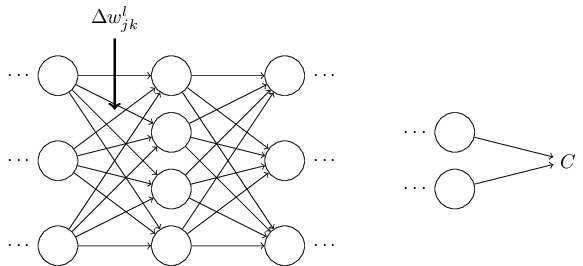
\includegraphics[width=0.9\textwidth]{images/tikz22.png}
\end{center}

\noindent 权重的这个改变将导致相应神经元的输出激活值发生变化：

\begin{center}
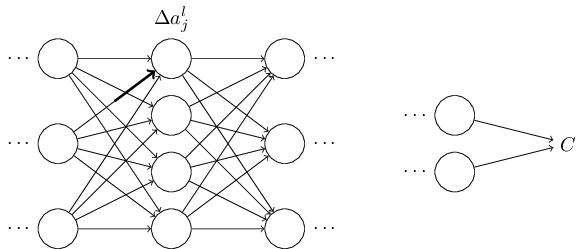
\includegraphics[width=0.9\textwidth]{images/tikz23.png}
\end{center}

\noindent 这反过来又会导致下一层中所有激活值发生变化：

\begin{center}
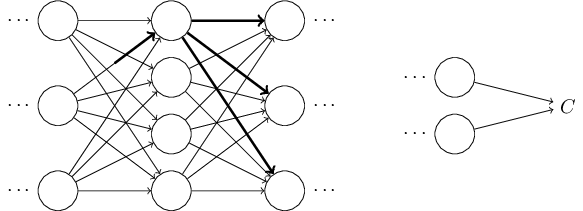
\includegraphics[width=0.9\textwidth]{images/tikz24.png}
\end{center}

\noindent 这些变化又会依次导致下一层发生变化，然后是再下一层，如此一直下去，直到导致最终层发生变化，进而导致代价函数发生变化：

\begin{center}
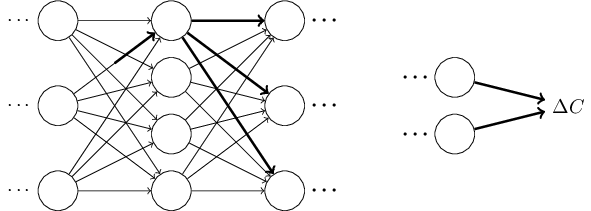
\includegraphics[width=0.9\textwidth]{images/tikz25.png}
\end{center}

\noindent 代价的变化 $\Delta C$ 与权重的变化 $\Delta w^l_{jk}$ 之间的关系由以下方程给出

\begin{equation}
\Delta C \approx \frac{\partial C}{\partial w^l_{jk}} \Delta w^l_{jk}.
\tag{47}
\end{equation}

\noindent 这表明，计算 $\frac{\partial C}{\partial w^l_{jk}}$ 的一种可能方法是仔细追踪 $w^l_{jk}$ 的微小变化如何传播并导致 $C$ 的微小变化. 如果我们能做到这一点，并且在此过程中小心地将一切都用易于计算的量来表示，那么我们就应该能够计算出 $\partial C / \partial w^l_{jk}$.

让我们试着来实现这一点. 变化 $\Delta w^l_{jk}$ 导致第 $l$ 层中第 $j$ 个神经元的激活值发生微小变化 $\Delta a^{l}_j$. 这个变化由下式给出

\begin{equation}
\Delta a^l_j \approx \frac{\partial a^l_j}{\partial w^l_{jk}} \Delta w^l_{jk}.
\tag{48}
\end{equation}

\noindent 激活值的变化 $\Delta a^l_{j}$ 将导致下一层，即第 $(l+1)$ 层中\emph{所有}激活值发生变化. 我们将集中讨论其中仅仅一个激活值受到影响的方式，比如 $a^{l+1}_q$，

\begin{center}
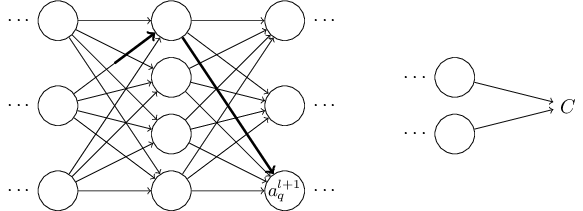
\includegraphics[width=0.9\textwidth]{images/tikz26.png}
\end{center}

\noindent 事实上，它将导致以下变化：

\begin{equation}
\Delta a^{l+1}_q \approx \frac{\partial a^{l+1}_q}{\partial a^l_j} \Delta a^l_j.
\tag{49}
\end{equation}

\noindent 代入方程 (48) 中的表达式

\begin{align*}
\Delta a^l_j \approx \frac{\partial a^l_j}{\partial w^l_{jk}} \Delta w^l_{jk} \nonumber
\end{align*}

\noindent，我们得到：

\begin{equation}
\Delta a^{l+1}_q \approx \frac{\partial a^{l+1}_q}{\partial a^l_j} \frac{\partial a^l_j}{\partial w^l_{jk}} \Delta w^l_{jk}.
\tag{50}
\end{equation}

\noindent 当然，变化 $\Delta a^{l+1}_q$ 又会依次导致下一层中激活值的变化. 事实上，我们可以想象一条从 $w^l_{jk}$ 到 $C$ 贯穿整个网络的路径，其中每一次激活值的变化都会导致下一个激活值的变化，最后导致输出端代价的变化. 如果这条路径经过激活值 $a^l_j, a^{l+1}_q, \ldots, a^{L-1}_n, a^L_m$，那么得到的表达式是

\begin{equation}
\Delta C \approx \frac{\partial C}{\partial a^L_m} \frac{\partial a^L_m}{\partial a^{L-1}_n} \frac{\partial a^{L-1}_n}{\partial a^{L-2}_p} \ldots \frac{\partial a^{l+1}_q}{\partial a^l_j} \frac{\partial a^l_j}{\partial w^l_{jk}} \Delta w^l_{jk},
\tag{51}
\end{equation}

\noindent 也就是说，对于我们经过的每一个额外的神经元，我们都获得了一个 $\partial a / \partial a$ 类型的项，以及最后的 $\partial C/\partial a^L_m$ 项. 这代表了由于沿着这条特定路径通过网络时激活值的变化所引起的 $C$ 的变化. 当然，$w^l_{jk}$ 的变化可以通过许多路径传播并影响代价，而我们只考虑了单条路径. 为了计算 $C$ 的总变化，我们似乎应该对权重和最终代价之间所有可能的路径求和，即

\begin{equation}
\Delta C \approx \sum_{mnp\ldots q} \frac{\partial C}{\partial a^L_m} \frac{\partial a^L_m}{\partial a^{L-1}_n} \frac{\partial a^{L-1}_n}{\partial a^{L-2}_p} \ldots \frac{\partial a^{l+1}_q}{\partial a^l_j} \frac{\partial a^l_j}{\partial w^l_{jk}} \Delta w^l_{jk},
\tag{52}
\end{equation}

\noindent 其中我们对路径上所有可能的中间神经元选择进行了求和. 与 (47) 比较

\begin{align*}
\Delta C \approx \frac{\partial C}{\partial w^l_{jk}} \Delta w^l_{jk} \nonumber
\end{align*}

\noindent 我们看到

\begin{equation}
\frac{\partial C}{\partial w^l_{jk}} = \sum_{mnp\ldots q} \frac{\partial C}{\partial a^L_m} \frac{\partial a^L_m}{\partial a^{L-1}_n} \frac{\partial a^{L-1}_n}{\partial a^{L-2}_p} \ldots \frac{\partial a^{l+1}_q}{\partial a^l_j} \frac{\partial a^l_j}{\partial w^l_{jk}}.
\tag{53}
\end{equation}

\noindent 现在，方程 (53)

\begin{align*}
\frac{\partial C}{\partial w^l_{jk}} = \sum_{mnp\ldots q} \frac{\partial C}{\partial a^L_m} \frac{\partial a^L_m}{\partial a^{L-1}_n} \frac{\partial a^{L-1}_n}{\partial a^{L-2}_p} \ldots \frac{\partial a^{l+1}_q}{\partial a^l_j} \frac{\partial a^l_j}{\partial w^l_{jk}} \nonumber
\end{align*}

\noindent 看起来很复杂. 然而，它有一个很好的直观解释. 我们正在计算 $C$ 相对于网络中某个权重的变化率. 这个方程告诉我们的是，网络中两个神经元之间的每条边都关联着一个速率因子，它就是一个神经元的激活值相对于另一个神经元激活值的偏导数. 从第一个权重到第一个神经元的边有一个速率因子 $\partial a^{l}_j / \partial w^l_{jk}$. 一条路径的速率因子就是沿着该路径的速率因子的乘积. 而总的变化率 $\partial C / \partial w^l_{jk}$ 就是从初始权重到最终代价的所有路径的速率因子之和. 这个过程在此处针对单条路径进行了说明：

\begin{center}
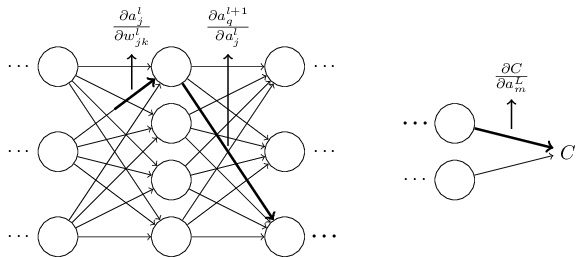
\includegraphics[width=0.9\textwidth]{images/tikz27.png}
\end{center}

\noindent 到目前为止，我提供的是一种启发式论证，一种思考当你扰动网络中的权重时发生了什么的方式. 让我勾勒出一条你可以用来进一步发展这个论证的思路. 首先，你可以推导出方程 (53) 中所有各个偏导数的显式表达式

\begin{align*}
\frac{\partial C}{\partial w^l_{jk}} = \sum_{mnp\ldots q} \frac{\partial C}{\partial a^L_m} \frac{\partial a^L_m}{\partial a^{L-1}_n} \frac{\partial a^{L-1}_n}{\partial a^{L-2}_p} \ldots \frac{\partial a^{l+1}_q}{\partial a^l_j} \frac{\partial a^l_j}{\partial w^l_{jk}} \nonumber
\end{align*}

\noindent. 用一点微积分很容易做到这一点. 完成之后，你可以尝试弄清楚如何将所有对指标的求和写成矩阵乘法. 事实证明这很繁琐，需要一些毅力，但不需要非凡的洞察力. 在做完所有这些，然后尽可能简化之后，你会发现你最终得到的正是反向传播算法！因此，你可以把反向传播算法看作提供了一种计算所有这些路径的速率因子之和的方法. 或者，稍微换个说法，反向传播算法是一种巧妙的方法，用于追踪权重（和偏置）的微小扰动在通过网络传播、到达输出、进而影响代价的过程.

现在，我不打算在这里把这一切都过一遍. 这很混乱，需要相当小心才能处理完所有细节. 如果你愿意接受挑战，你可能会喜欢尝试一下. 即使不愿意，我也希望这条思路能让你对反向传播所取得的成就有所领悟.

那么另一个谜团呢——反向传播最初是如何被发现的？事实上，如果你遵循我刚才勾勒的方法，你会发现反向传播的一个证明. 不幸的是，这个证明比我在本章前面描述的那个要长得多，也复杂得多. 那么，那个简短（但更神秘）的证明是如何被发现的呢？当你写出长证明的所有细节时，你会发现，事后看来，有几个明显的简化就摆在眼前. 你做出那些简化，得到一个更短的证明，并把它写出来. 然后又有几个明显的简化跳出来. 于是你再次重复. 经过几次迭代后得到的结果就是我们之前看到的证明*\footnote{这里需要一个巧妙的步骤. 在方程 (53) $\frac{\partial C}{\partial w^l_{jk}} = \sum_{mnp\ldots q} \frac{\partial C}{\partial a^L_m} \frac{\partial a^L_m}{\partial a^{L-1}_n} \frac{\partial a^{L-1}_n}{\partial a^{L-2}_p} \ldots \frac{\partial a^{l+1}_q}{\partial a^l_j} \frac{\partial a^l_j}{\partial w^l_{jk}}$ 中，中间变量是像 $a_q^{l+1}$ 这样的激活值. 巧妙的想法是改用加权输入，比如 $z^{l+1}_q$，作为中间变量. 如果你没有这个想法，而是继续使用激活值 $a^{l+1}_q$，你得到的证明结果会比本章前面给出的证明稍微复杂一些.}——简短，但有些晦涩，因为所有指向其构造的路标都被移除了！当然，我是在请求你相信我这一点，但早期证明的起源确实没有什么大的谜团. 它只是大量艰苦的工作，简化了我在本节中勾勒的证明.

\chapter{改进神经网络的学习方式}
当高尔夫球手第一次学习打高尔夫球时，他们通常把大部分时间花在练习基本的挥杆动作上. 只有在基本挥杆的基础上逐步发展，他们才会学习其他击球方式，学会切球、左曲球和右曲球，并对基本挥杆进行改进和调整. 类似地，到目前为止，我们一直专注于理解反向传播算法. 它是我们的``基本挥杆''，是大多数神经网络工作中学习的基础. 在本章中，我将介绍一套技术，可以用来改进我们朴素实现的反向传播，从而改进网络的学习方式.

我们将在本章中介绍的技术包括：更好的代价函数选择，即所谓的交叉熵\label{term:50}代价函数；四种所谓的``正则化\label{term:52}''方法（L1 和 L2 正则化、dropout，以及训练数据的人工扩展），它们使我们的网络在训练数据之外具有更好的泛化\label{term:51}能力；更好的网络权重初始化方法；以及一组帮助选择良好网络超参数的启发式方法. 我还会简要概述其他几种技术. 这些讨论在很大程度上彼此独立，因此如果你愿意，可以跳着阅读. 我们还会在可运行的代码中实现许多技术，并用它们来改进第 1 章中研究的手写数字分类问题所得到的结果.

当然，我们只涵盖了为神经网络开发的众多技术中的一小部分. 其理念是，进入大量可用技术的最佳途径是深入研究其中最重要的几项. 掌握这些重要技术不仅本身有用，还会加深你对使用神经网络时可能出现的各种问题的理解. 这将使你做好充分准备，在需要时快速掌握其他技术.
\sectionTitle{交叉熵代价函数}{交叉熵代价函数}

我们大多数人都觉得犯错令人不快. 刚开始学钢琴不久，我就在观众面前进行了第一次表演. 我很紧张，结果把曲子弹低了一个八度. 我慌了神，直到有人指出我的错误才继续下去. 我非常尴尬. 然而，尽管令人不快，当我们错得离谱时，我们也能很快学到东西. 你可以打赌，下一次我在观众面前演奏时，一定弹在了正确的八度上！相比之下，当我们的错误不那么明确时，我们学得就比较慢.

理想情况下，我们希望并期待我们的神经网络能够从错误中快速学习. 实际情况是这样吗？为了回答这个问题，让我们看一个玩具模型\label{term:53}. 这个例子涉及一个只有一个输入的神经元：

\begin{center}
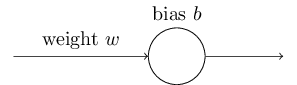
\includegraphics[width=0.9\textwidth]{images/tikz28.png}
\end{center}

\noindent 我们将训练这个神经元做一件简单得可笑的事：把输入 $1$ 变成输出 $0$. 当然，这是一个如此微不足道的任务，我们不用学习算法就能轻易地手算出合适的权重和偏置. 然而，用梯度下降来尝试学习权重和偏置却很有启发性. 所以让我们来看看这个神经元是如何学习的.

为了明确起见，我把初始权重设为 $0.6$，初始偏置设为 $0.9$. 这些是作为学习起点的通用选择，我并没有特意挑选它们. 神经元的初始输出是 $0.82$，所以在我们的神经元接近期望输出 $0.0$ 之前，需要进行相当多的学习. 点击下面右下角的 ``Run'' 来看看神经元如何学习到一个更接近 $0.0$ 的输出. 注意这不是预先录制的动画，你的浏览器实际上在计算梯度，然后用梯度更新权重和偏置，并显示结果. 学习率是 $\eta = 0.15$，事实证明这足够慢，让我们能跟上发生了什么，但又足够快，让我们在几秒钟内就能取得实质性的学习. 代价函数是第 1 章介绍的二次代价函数 $C$. 我很快就会提醒你代价函数的确切形式，所以不必去翻找定义. 注意你可以再次点击 ``Run'' 来多次运行动画.

如你所见，神经元迅速学到了一个权重和偏置，使代价下降，并使神经元的输出约为 $0.09$. 这并不完全是期望的输出 $0.0$，但已经相当不错了. 然而，假设我们改为把起始权重和起始偏置都设为 $2.0$. 在这种情况下，初始输出是 $0.98$，错得非常离谱. 让我们看看在这种情况下神经元如何学习输出 $0$. 再次点击 ``Run''：尽管这个例子使用了相同的学习率 ($\eta = 0.15$)，我们可以看到学习开始得慢得多. 事实上，在前 150 个左右的轮次中，权重和偏置几乎完全没有变化. 然后学习才开始起作用，并且和我们的第一个例子很像，神经元的输出迅速向 $0.0$ 靠近.

与人类学习相比，这种行为很奇怪. 正如我在本节开头所说，当我们对某件事错得很离谱时，我们往往学得最快. 但我们刚刚看到，我们的人工神经元在错得很离谱时学习有很大困难——比只是稍微错一点时困难得多. 更重要的是，事实证明这种行为不仅出现在这个玩具模型中，也出现在更一般的网络中. 为什么学习如此缓慢？我们能否找到一种避免这种减速的方法？

要理解这个问题的根源，请考虑我们的神经元是通过以由代价函数的偏导数 $\partial C/\partial w$ 和 $\partial C / \partial b$ 决定的速率改变权重和偏置来学习的. 所以，说 ``学习缓慢'' 实际上就等于说那些偏导数很小. 挑战在于理解它们为什么很小. 为了理解这一点，让我们计算这些偏导数. 回想一下，我们使用的是二次代价函数，根据方程 (6)

\begin{align*}
C(w,b) \equiv \frac{1}{2n} \sum_x \| y(x) - a\|^2 \nonumber
\end{align*}

\noindent，它由下式给出

\begin{equation}
C = \frac{(y-a)^2}{2},
\tag{54}
\end{equation}

\noindent 其中 $a$ 是使用训练输入 $x = 1$ 时神经元的输出，而 $y = 0$ 是对应的期望输出. 为了用权重和偏置更明确地写出这一点，回想一下 $a = \sigma(z)$，其中 $z = wx+b$. 使用链式法则对权重和偏置求导，我们得到

\begin{align}
\frac{\partial C}{\partial w} &= (a-y)\sigma'(z) x = a \sigma'(z) \tag{55} \\ \frac{\partial C}{\partial b} &= (a-y)\sigma'(z) = a \sigma'(z), \tag{56}
\end{align}

\noindent 其中我已代入 $x = 1$ 和 $y = 0$. 为了理解这些表达式的行为，让我们更仔细地看看右边的 $\sigma'(z)$ 项. 回想一下 $\sigma$ 函数的形状：我们可以从这个图中看到，当神经元的输出接近 $1$ 时，曲线变得非常平坦，因此 $\sigma'(z)$ 变得非常小. 方程 (55)

\begin{align*}
\frac{\partial C}{\partial w} &= (a-y)\sigma'(z) x = a \sigma'(z) \nonumber
\end{align*}

\noindent 和 (56)

\begin{align*}
\frac{\partial C}{\partial b} &= (a-y)\sigma'(z) = a \sigma'(z) \nonumber
\end{align*}

\noindent 然后告诉我们 $\partial C / \partial w$ 和 $\partial C / \partial b$ 变得非常小. 这就是学习缓慢的根源. 更重要的是，正如我们稍后将看到的，在更一般的神经网络中，学习缓慢的发生原因本质上相同，而不仅仅是我们一直在玩的这个玩具例子.
\subsectionTitle{交叉熵代价函数入门}{交叉熵代价函数入门}

我们如何解决学习缓慢的问题？事实证明，我们可以通过将二次代价替换为另一种称为交叉熵的代价函数来解决这个问题. 为了理解交叉熵，让我们稍微离开那个超级简单的玩具模型. 我们改为假设我们试图训练一个具有多个输入变量的神经元，$x_1, x_2, \ldots$，对应的权重 $w_1, w_2, \ldots$，以及一个偏置 $b$：

\begin{center}
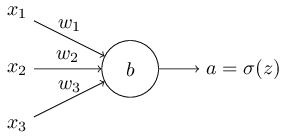
\includegraphics[width=0.9\textwidth]{images/tikz29.png}
\end{center}

\noindent 神经元的输出当然是 $a = \sigma(z)$，其中 $z = \sum_j w_j x_j+b$ 是输入的加权和. 我们为这个神经元定义交叉熵代价函数为

\begin{equation}
C = -\frac{1}{n} \sum_x \left[y \ln a + (1-y ) \ln (1-a) \right],
\tag{57}
\end{equation}

\noindent 其中 $n$ 是训练数据项的总数，求和是对所有训练输入 $x$ 进行的，而 $y$ 是对应的期望输出.

表达式 (57)

\begin{align*}
C = -\frac{1}{n} \sum_x \left[y \ln a + (1-y ) \ln (1-a) \right] \nonumber
\end{align*}

\noindent 能解决学习缓慢问题这一点并不明显. 事实上，坦率地说，把它称为代价函数是否合理甚至都不明显！在解决学习缓慢问题之前，让我们看看交叉熵在什么意义上可以被解释为代价函数.

有两个性质特别使得将交叉熵解释为代价函数是合理的. 首先，它是非负的，即 $C > 0$. 要看到这一点，请注意：(a) (57) 中求和里的所有各项

\begin{align*}
C = -\frac{1}{n} \sum_x \left[y \ln a + (1-y ) \ln (1-a) \right] \nonumber
\end{align*}

\noindent 都是负的，因为两个对数都是 $0$ 到 $1$ 范围内的数；并且 (b) 求和前面有一个负号.

其次，如果神经元对所有训练输入 $x$ 的实际输出都接近期望输出，那么交叉熵将接近零*\footnote{为了证明这一点，我需要假设期望输出 $y$ 都是 $0$ 或 $1$. 在解决分类问题时，例如，或者在计算布尔函数时，通常就是这种情况. 要理解当我们不做这个假设时会发生什么，请参见本节末尾的练习.}. 要看到这一点，例如假设对于某个输入 $x$，$y = 0$ 且 $a \approx 0$. 这是神经元在该输入上表现良好的情况. 我们看到代价表达式 (57)

\begin{align*}
C = -\frac{1}{n} \sum_x \left[y \ln a + (1-y ) \ln (1-a) \right] \nonumber
\end{align*}

\noindent 中的第一项消失了，因为 $y = 0$，而第二项就是 $-\ln (1-a) \approx 0$. 当 $y = 1$ 且 $a \approx 1$ 时也有类似的分析. 因此，只要实际输出接近期望输出，对代价的贡献就会很低.

总结起来，交叉熵是正的，并且当神经元对所有训练输入 $x$ 计算期望输出 $y$ 的能力越来越好时，它趋向于零. 这两个性质都是我们直觉上期望代价函数具有的. 事实上，二次代价也满足这两个性质. 所以这对交叉熵来说是个好消息. 但交叉熵代价函数的优点在于，与二次代价不同，它避免了学习减慢的问题. 要看到这一点，让我们计算交叉熵代价关于权重的偏导数. 我们将 $a = \sigma(z)$ 代入 (57)

\begin{align*}
C = -\frac{1}{n} \sum_x \left[y \ln a + (1-y ) \ln (1-a) \right] \nonumber
\end{align*}

\noindent，并应用两次链式法则，得到：

\begin{align}
\frac{\partial C}{\partial w_j} &= -\frac{1}{n} \sum_x \left( \frac{y }{\sigma(z)} -\frac{(1-y)}{1-\sigma(z)} \right) \frac{\partial \sigma}{\partial w_j} \tag{58} \\ &= -\frac{1}{n} \sum_x \left( \frac{y}{\sigma(z)} -\frac{(1-y)}{1-\sigma(z)} \right)\sigma'(z) x_j. \tag{59}
\end{align}

\noindent 将所有项放在公分母上并化简后，这变为：

\begin{equation}
\frac{\partial C}{\partial w_j} = \frac{1}{n} \sum_x \frac{\sigma'(z) x_j}{\sigma(z) (1-\sigma(z))} (\sigma(z)-y).
\tag{60}
\end{equation}

\noindent 利用 S 型函数的定义 $\sigma(z) = 1/(1+e^{-z})$，以及一点代数运算，我们可以证明 $\sigma'(z) = \sigma(z)(1-\sigma(z))$. 我会在下面的练习中请你验证这一点，但现在让我们暂且接受它. 我们看到 $\sigma'(z)$ 和 $\sigma(z)(1-\sigma(z))$ 项在上面的方程中相互抵消了，它简化为：

\begin{equation}
\frac{\partial C}{\partial w_j} = \frac{1}{n} \sum_x x_j(\sigma(z)-y).
\tag{61}
\end{equation}

\noindent 这是一个漂亮的表达式. 它告诉我们权重学习的速度由 $\sigma(z)-y$ 控制，即由输出中的误差控制. 误差越大，神经元学习得越快. 这正是我们直觉上期望的. 特别地，它避免了由二次代价的类似方程，即方程 (55)

\begin{align*}
\frac{\partial C}{\partial w} &= (a-y)\sigma'(z) x = a \sigma'(z) \nonumber
\end{align*}

\noindent 中的 $\sigma'(z)$ 项所导致的学习减慢. 当我们使用交叉熵时，$\sigma'(z)$ 项被抵消了，我们不再需要担心它很小. 这种抵消是交叉熵代价函数所保证的特殊奇迹. 实际上，这并不真的是一个奇迹. 正如我们稍后将看到的，交叉熵被特别选择正是为了具有这个性质.

以类似的方式，我们可以计算偏置的偏导数. 我不会再详细讲述所有细节，但你可以很容易地验证

\begin{equation}
\frac{\partial C}{\partial b} = \frac{1}{n} \sum_x (\sigma(z)-y).
\tag{62}
\end{equation}

\noindent 同样，这避免了由二次代价的类似方程，即方程 (56)

\begin{align*}
\frac{\partial C}{\partial b} &= (a-y)\sigma'(z) = a \sigma'(z) \nonumber
\end{align*}

\noindent 中的 $\sigma'(z)$ 项所导致的学习减慢.

\begin{exerciseBox}{练习}

\begin{itemize}

\item 验证 $\sigma'(z) = \sigma(z)(1-\sigma(z))$.

\end{itemize}

让我们回到之前玩过的玩具例子，探索当我们使用交叉熵而不是二次代价时会发生什么. 为了重新定位自己，我们将从二次代价表现良好的情况开始，起始权重为 $0.6$，起始偏置为 $0.9$. 按下 ``Run'' 看看当我们用交叉熵替换二次代价时会发生什么：不出所料，神经元在这个例子中学习得非常好，就像之前一样. 现在让我们看看我们的神经元之前卡住的情况（链接，用于比较），权重和偏置都从 $2.0$ 开始：成功了！这一次神经元学习得很快，正如我们所希望的那样. 如果你仔细观察，你可以看到代价曲线的斜率最初比二次代价对应曲线上初始平坦区域要陡峭得多. 正是这种陡峭性，交叉熵为我们带来的，防止我们在期望神经元学习最快的时候卡住，即当神经元一开始就错得离谱的时候.

我没有说明刚才展示的例子中使用了什么学习率. 之前，使用二次代价时，我们使用了 $\eta = 0.15$. 我们在新例子中应该使用相同的学习率吗？事实上，随着代价函数的改变，不可能精确地说使用 ``相同'' 学习率意味着什么；这是苹果和橘子的比较. 对于两种代价函数，我都只是通过实验来找到一个能够看清发生了什么事情的学习率. 如果你仍然好奇，尽管我否认了，这里是内幕：在刚才给出的例子中我使用了 $\eta = 0.005$.

你可能会反对说，学习率的变化使得上面的图变得毫无意义. 当我们的学习率选择一开始就是任意的时候，谁在乎神经元学习得有多快呢？！这种反对没有抓住要点. 这些图的要点不在于学习的绝对速度. 而在于学习速度如何变化. 特别地，当我们使用二次代价时，当神经元明显错误时学习比之后当神经元更接近正确输出时\emph{更慢}；而使用交叉熵时，当神经元明显错误时学习更快. 这些陈述不依赖于学习率是如何设置的.

我们一直在研究单个神经元的交叉熵. 然而，很容易将交叉熵推广到多神经元多层网络. 特别地，假设 $y = y_1, y_2, \ldots$ 是输出神经元，即最终层神经元的期望值，而 $a^L_1, a^L_2, \ldots$ 是实际输出值. 那么我们定义交叉熵为

\begin{equation}
C = -\frac{1}{n} \sum_x \sum_j \left[y_j \ln a^L_j + (1-y_j) \ln (1-a^L_j) \right].
\tag{63}
\end{equation}

\noindent 这与我们之前的表达式，即方程 (57)

\begin{align*}
C = -\frac{1}{n} \sum_x \left[y \ln a + (1-y ) \ln (1-a) \right] \nonumber
\end{align*}

\noindent 相同，只是现在我们用 $\sum_j$ 对所有输出神经元求和. 我不会明确地推导，但使用表达式 (63)

\begin{align*}
C = -\frac{1}{n} \sum_x \sum_j \left[y_j \ln a^L_j + (1-y_j) \ln (1-a^L_j) \right] \nonumber
\end{align*}

\noindent 在多神经元网络中避免学习减慢应该是合理的. 如果你感兴趣，你可以在下面的习题中进行推导.

顺便说一句，我使用 ``交叉熵'' 这个术语的方式让一些早期读者感到困惑，因为它表面上似乎与其他来源冲突. 特别地，通常将两个概率分布 $p_j$ 和 $q_j$ 的交叉熵定义为 $\sum_j p_j \ln q_j$. 这个定义可能与 (57)

\begin{align*}
C = -\frac{1}{n} \sum_x \left[y \ln a + (1-y ) \ln (1-a) \right] \nonumber
\end{align*}

\noindent 相关，如果我们把单个 S 型神经元视为输出一个由神经元的激活值 $a$ 及其补 $1-a$ 组成的概率分布.

然而，当我们在最终层有许多 S 型神经元时，激活值的向量 $a^L_j$ 通常不构成概率分布. 因此，像 $\sum_j p_j \ln q_j$ 这样的定义甚至没有意义，因为我们不是在处理概率分布. 相反，你可以把 (63)

\begin{align*}
C = -\frac{1}{n} \sum_x \sum_j \left[y_j \ln a^L_j + (1-y_j) \ln (1-a^L_j) \right] \nonumber
\end{align*}

\noindent 看作是一组逐神经元交叉熵的总和，每个神经元的激活值被解释为二元概率分布的一部分*\footnote{当然，在我们的网络中没有概率元素，所以它们不是真正的概率.}. 在这个意义上，(63)

\begin{align*}
C = -\frac{1}{n} \sum_x \sum_j \left[y_j \ln a^L_j + (1-y_j) \ln (1-a^L_j) \right] \nonumber
\end{align*}

\noindent 是概率分布交叉熵的推广.

我们什么时候应该使用交叉熵而不是二次代价？事实上，只要输出神经元是 S 型神经元，交叉熵几乎总是更好的选择. 要理解为什么，考虑当我们建立网络时，我们通常使用某种随机化来初始化权重和偏置. 可能发生的情况是，那些初始选择导致网络对某些训练输入决定性地错误——也就是说，一个输出神经元将在应该为 $0$ 时饱和在 $1$ 附近，或者反之. 如果我们使用二次代价，那将减慢学习. 它不会完全停止学习，因为权重将继续从其他训练输入中学习，但这显然是不可取的.

\end{exerciseBox}
\begin{exerciseBox}{练习}

\begin{itemize}

\item 交叉熵的一个容易出错之处在于，一开始很难记住 $y$ 和 $a$ 各自扮演的角色. 人们很容易搞混正确的形式究竟是 $-[y \ln a + (1-y) \ln (1-a)]$ 还是 $-[a \ln y + (1-a) \ln (1-y)]$. 当 $y = 0$ 或 $1$ 时，第二个表达式会发生什么？第一个表达式是否也有这个问题？为什么有或为什么没有？

\item
在本节开头的单神经元讨论中，我论证了如果对所有训练输入都有 $\sigma(z) \approx y$，那么交叉熵就很小. 该论证依赖于 $y$ 等于 $0$ 或 $1$. 这在分类问题中通常是成立的，但对于其他问题（例如回归问题），$y$ 有时可能取介于 $0$ 和 $1$ 之间的值. 证明当对所有训练输入都有 $\sigma(z) = y$ 时，交叉熵仍然取最小值. 在这种情况下，交叉熵的值为：

\begin{equation}
C = -\frac{1}{n} \sum_x [y \ln y+(1-y) \ln(1-y)].
\tag{64}
\end{equation}

量 $-[y \ln y+(1-y)\ln(1-y)]$ 有时被称为二元熵.

\end{itemize}

\end{exerciseBox}

\begin{exerciseBox}{习题}

\begin{itemize}

\item
\textbf{多层多神经元网络} 用上一章引入的记号，证明对于二次代价，关于输出层权重的偏导数为

\begin{equation}
\frac{\partial C}{\partial w^L_{jk}} = \frac{1}{n} \sum_x a^{L-1}_k (a^L_j-y_j) \sigma'(z^L_j).
\tag{65}
\end{equation}

项 $\sigma'(z^L_j)$ 会在输出神经元在错误的值上饱和时导致学习变慢. 证明对于交叉熵代价，单个训练样本 $x$ 的输出误差 $\delta^L$ 为

\begin{equation}
\delta^L = a^L-y.
\tag{66}
\end{equation}

利用这个表达式证明关于输出层权重的偏导数为

\begin{equation}
\frac{\partial C}{\partial w^L_{jk}} = \frac{1}{n} \sum_x a^{L-1}_k (a^L_j-y_j).
\tag{67}
\end{equation}

$\sigma'(z^L_j)$ 项消失了，因此交叉熵避免了学习变慢的问题，不仅像我们之前看到的那样在用于单个神经元时如此，而且在多层多神经元网络中也是如此. 对这一分析稍作变化也适用于偏置. 如果这对你来说不明显，那么你也应该把那个分析推导一遍.

\item
\textbf{当输出层是线性神经元时使用二次代价} 假设我们有一个多层多神经元网络. 假设最后一层中的所有神经元都是 \emph{线性神经元}，这意味着没有应用 S 型激活函数，输出就是 $a^L_j = z^L_j$. 证明如果我们使用二次代价函数，那么单个训练样本 $x$ 的输出误差 $\delta^L$ 为

\begin{equation}
\delta^L = a^L-y.
\tag{68}
\end{equation}

与上一个习题类似，利用这个表达式证明关于输出层权重和偏置的偏导数为

\begin{align}
\frac{\partial C}{\partial w^L_{jk}} &= \frac{1}{n} \sum_x a^{L-1}_k (a^L_j-y_j) \tag{69} \\ \frac{\partial C}{\partial b^L_{j}} &= \frac{1}{n} \sum_x (a^L_j-y_j). \tag{70}
\end{align}

这表明如果输出神经元是线性神经元，那么二次代价不会引起任何学习变慢的问题. 在这种情况下，二次代价实际上是一个合适使用的代价函数.

\end{itemize}

\end{exerciseBox}
\subsectionTitle{用交叉熵分类 MNIST 数字}{用交叉熵分类 MNIST 数字}

交叉熵很容易作为使用梯度下降和反向传播进行学习的程序的一部分来实现. 我们将在本章后面这样做，开发我们之前用于分类 MNIST 手写数字的程序 \texttt{network.py} 的改进版本. 新程序称为 \texttt{network2.py}，它不仅包含交叉熵，还包含本章中开发的若干其他技术*\footnote{代码可在 GitHub 上获取.}. 现在，让我们看看我们的新程序分类 MNIST 数字的效果如何. 与第 1 章的情况一样，我们将使用一个有 $30$ 个隐藏神经元的网络，并使用 $10$ 的小批量大小. 我们将学习率设为 $\eta = 0.5$*\footnote{在第 1 章中我们使用了二次代价和学习率 $\eta = 3.0$. 如上所述，当代价函数改变时，无法确切说明使用``相同''学习率意味着什么. 对于这两种代价函数，我都进行了实验，以在给定其他超参数选择的情况下找到能提供接近最优性能的学习率. \\ \\ 顺便说一句，对于将交叉熵的学习率与二次代价的学习率联系起来，有一个非常粗略的一般性经验法则. 正如我们之前看到的，二次代价的梯度项中多了一个 $\sigma' = \sigma(1-\sigma)$ 项. 假设我们对 $\sigma$ 的取值求平均，$\int_0^1 d\sigma \sigma(1-\sigma) = 1/6$. 我们看到（非常粗略地），在相同学习率下，二次代价的学习速度平均慢 $6$ 倍. 这表明一个合理的起点是将二次代价的学习率除以 $6$. 当然，这个论证远非严格，不应过于当真. 尽管如此，它有时可以是一个有用的起点.} 并训练 $30$ 个轮次. \texttt{network2.py} 的接口与 \texttt{network.py} 略有不同，但应该仍然清楚发生了什么. 顺便说一句，你可以通过在 Python shell 中使用诸如 \texttt{help(network2.Network.SGD)} 之类的命令来获取关于 \texttt{network2.py} 接口的文档.

\begin{lstlisting}
>>> import mnist_loader
>>> training_data, validation_data, test_data = \
... mnist_loader.load_data_wrapper()
>>> import network2
>>> net = network2.Network([784, 30, 10], cost=network2.CrossEntropyCost)
>>> net.large_weight_initializer()
>>> net.SGD(training_data, 30, 10, 0.5, evaluation_data=test_data,
... monitor_evaluation_accuracy=True)

\end{lstlisting}

顺便注意，\texttt{net.large\_\allowbreak{}weight\_\allowbreak{}initializer()} 命令用于以与第 1 章所述相同的方式初始化权重和偏置. 我们需要运行这个命令，因为在本章后面我们将改变网络中默认的权重初始化. 运行上述命令序列的结果是一个准确率为 $95.49$ 百分比的网络. 这与我们在第 1 章中使用二次代价得到的结果 $95.42$ 百分比非常接近.

让我们也看看使用 $100$ 个隐藏神经元、交叉熵，而其他参数保持不变的情况. 在这种情况下，我们获得了 $96.82$ 百分比的准确率. 这比第 1 章的结果有了实质性的改进，当时我们使用二次代价获得了 $96.59$ 百分比的分类准确率. 这看起来可能变化很小，但考虑到错误率已从 $3.41$ 百分比降至 $3.18$ 百分比. 也就是说，我们消除了大约十四分之一的原始错误. 这是相当可观的改进.

令人鼓舞的是，交叉熵代价给出的结果与二次代价相似或更好. 然而，这些结果并不能确凿地证明交叉熵是更好的选择. 原因是我只花了很少的精力来选择诸如学习率、小批量大小等超参数. 要使这种改进真正令人信服，我们需要对这些超参数进行彻底的优化. 尽管如此，这些结果是令人鼓舞的，并强化了我们早先的理论论证，即交叉熵比二次代价是更好的选择.

顺便说一句，这是我们在本章乃至本书其余大部分内容中将会看到的一种普遍模式的一部分. 我们将开发一项新技术，尝试它，然后得到``改进的''结果. 当然，看到这样的改进是很好的. 但对此类改进的解释总是有问题的. 只有当我们付出巨大努力优化所有其他超参数后看到改进，它们才真正令人信服. 那是大量的工作，需要大量的计算能力，而我们通常不会进行如此详尽的调查. 相反，我们将基于像上面所做的那样的非正式测试继续进行. 尽管如此，你应该记住，此类测试达不到确凿的证明，并保持警惕，留意论证正在失效的迹象.

到目前为止，我们已经详细讨论了交叉熵. 既然它只给我们的 MNIST 结果带来很小的改进，为什么要付出这么多努力呢？在本章后面，我们将看到其他技术——特别是正则化——能带来更大的改进. 那么为什么如此关注交叉熵呢？部分原因是交叉熵是一种广泛使用的代价函数，因此值得好好理解. 但更重要的原因是，神经元饱和是神经网络中的一个重要问题，我们将在本书中反复回到这个问题. 因此，我详细讨论了交叉熵，因为它是一个很好的实验室，可以用来开始理解神经元饱和以及如何解决它.
\subsectionTitle{交叉熵是什么意思？从何而来？}{交叉熵是什么意思？从何而来？}

我们对交叉熵的讨论集中在代数分析和实际实现上. 这很有用，但它留下了一些更广泛的概念性问题没有回答，比如：交叉熵是什么意思？有没有某种直观的方式来思考交叉熵？以及我们最初是如何想到交叉熵的？

让我们从最后一个问题开始：最初是什么促使我们想到交叉熵的？假设我们已经发现了前面描述的学习缓慢现象，并且理解了其根源是方程 (55)

\begin{align*}
\frac{\partial C}{\partial w} &= (a-y)\sigma'(z) x = a \sigma'(z) \nonumber
\end{align*}

\noindent 和 (56)

\begin{align*}
\frac{\partial C}{\partial b} &= (a-y)\sigma'(z) = a \sigma'(z) \nonumber
\end{align*}

\noindent 中的 $\sigma'(z)$ 项. 盯着这些方程看一会儿之后，我们可能会想，是否有可能选择一个代价函数，使得 $\sigma'(z)$ 项消失. 在这种情况下，单个训练样本 $x$ 的代价 $C = C_x$ 将满足

\begin{align}
\frac{\partial C}{\partial w_j} &= x_j(a-y) \tag{71} \\ \frac{\partial C}{\partial b } &= (a-y). \tag{72}
\end{align}

\noindent 如果我们能选择代价函数使这些方程成立，那么它们将以一种简单的方式捕捉到这样一个直觉：初始误差越大，神经元学习得越快. 它们还将消除学习缓慢的问题. 事实上，从这些方程出发，我们现在将展示，仅仅通过跟随我们的数学直觉，就有可能推导出交叉熵的形式. 为了看到这一点，注意由链式法则我们有

\begin{equation}
\frac{\partial C}{\partial b} = \frac{\partial C}{\partial a} \sigma'(z).
\tag{73}
\end{equation}

\noindent 利用 $\sigma'(z) = \sigma(z)(1-\sigma(z)) = a(1-a)$，最后一个方程变为

\begin{equation}
\frac{\partial C}{\partial b} = \frac{\partial C}{\partial a} a(1-a).
\tag{74}
\end{equation}

\noindent 与方程 (72)

\begin{align*}
\frac{\partial C}{\partial b } &= (a-y) \nonumber
\end{align*}

\noindent 比较，我们得到

\begin{equation}
\frac{\partial C}{\partial a} = \frac{a-y}{a(1-a)}.
\tag{75}
\end{equation}

\noindent 对这个表达式关于 $a$ 积分得到

\begin{equation}
C = -[y \ln a + (1-y) \ln (1-a)]+ {\rm constant},
\tag{76}
\end{equation}

\noindent 其中包含一个积分常数. 这是单个训练样本 $x$ 对代价的贡献. 要得到完整的代价函数，我们必须对训练样本取平均，得到

\begin{equation}
C = -\frac{1}{n} \sum_x [y \ln a +(1-y) \ln(1-a)] + {\rm constant},
\tag{77}
\end{equation}

\noindent 这里的常数是每个训练样本各自常数的平均值. 于是我们看到，方程 (71)

\begin{align*}
\frac{\partial C}{\partial w_j} &= x_j(a-y) \nonumber
\end{align*}

\noindent 和 (72)

\begin{align*}
\frac{\partial C}{\partial b } &= (a-y) \nonumber
\end{align*}

\noindent 唯一地确定了交叉熵的形式，至多相差一个整体常数项. 交叉熵并不是什么奇迹般从虚空中拽出来的东西. 相反，它是我们可以通过一种简单而自然的方式发现的东西.

那么交叉熵的直观含义呢？我们应该如何理解它？深入解释这一点会把我带到比我想去的更远的地方. 然而，值得一提的是，有一种来自信息论领域的标准方式来解释交叉熵. 粗略地说，这个想法是交叉熵是惊讶程度的一种度量. 特别地，我们的神经元试图计算函数 $x \rightarrow y = y(x)$. 但它实际计算的是函数 $x \rightarrow a = a(x)$. 假设我们把 $a$ 看作神经元对 $y$ 为 $1$ 的估计概率，而 $1-a$ 是对 $y$ 的正确值为 $0$ 的估计概率. 那么交叉熵衡量的是，当我们得知 $y$ 的真实值时，平均而言我们有多``惊讶''. 如果输出是我们所预期的，我们得到的惊讶程度就低；如果输出是出乎意料的，惊讶程度就高. 当然，我还没有确切说明``惊讶''是什么意思，所以这也许看起来像是空话. 但事实上，有一种精确的信息论方式来说明惊讶的含义. 不幸的是，我不知道网上有关于这个主题的好的、简短的、自包含的讨论. 但如果你想深入挖掘，维基百科上有一个简短的总结，可以让你走上正确的轨道. 而细节可以通过阅读 Cover 和 Thomas 关于信息论的书中第 5 章关于 Kraft 不等式的材料来补充.

\begin{exerciseBox}{习题}

\begin{itemize}

\item
我们已经详细讨论了在使用二次代价训练的网络中，输出神经元饱和时可能发生的学习缓慢现象. 另一个可能抑制学习的因素是方程 (61)

\begin{align*}
\frac{\partial C}{\partial w_j} = \frac{1}{n} \sum_x x_j(\sigma(z)-y) \nonumber
\end{align*}

中 $x_j$ 项的存在. 由于这一项，当输入 $x_j$ 接近零时，对应的权重 $w_j$ 将学习得很慢. 解释为什么不可能通过巧妙地选择代价函数来消除 $x_j$ 项.

\end{itemize}

\end{exerciseBox}
\subsectionTitle{Softmax}{Softmax}

在本章中，我们将主要使用交叉熵代价来解决学习缓慢的问题. 然而，我想简要地描述解决该问题的另一种方法，它基于所谓的 \emph{softmax} 神经元层. 在本章的剩余部分中，我们实际上不会使用 softmax 层，所以如果你非常着急，可以跳到下一节. 然而，softmax 仍然值得理解，部分原因是它本身很有趣，部分原因是我们在第 6 章讨论深度神经网络时会使用 softmax 层.

Softmax 的思想是为我们的神经网络定义一种新型的输出层. 它的开始方式与 S 型层相同，通过形成加权输入*\footnote{在描述 softmax 时，我们将频繁使用上一章引入的记号. 如果你需要回顾该章以刷新关于记号含义的记忆，不妨重读那一章.} $z^L_j = \sum_{k} w^L_{jk} a^{L-1}_k + b^L_j$. 然而，我们不应用 S 型函数来获得输出. 相反，在 softmax 层中，我们对 $z^L_j$ 应用所谓的 \emph{softmax 函数}. 根据这个函数，第 $j$ 个输出神经元的激活值 $a^L_j$ 是

\begin{equation}
a^L_j = \frac{e^{z^L_j}}{\sum_k e^{z^L_k}},
\tag{78}
\end{equation}

\noindent 其中分母是对所有输出神经元求和.

如果你不熟悉 softmax 函数，方程 (78)

\begin{align*}
a^L_j = \frac{e^{z^L_j}}{\sum_k e^{z^L_k}} \nonumber
\end{align*}

\noindent 可能看起来相当晦涩. 我们为什么想要使用这个函数当然并不明显. 而且这能帮助我们解决学习缓慢问题也不明显. 为了更好地理解方程 (78)

\begin{align*}
a^L_j = \frac{e^{z^L_j}}{\sum_k e^{z^L_k}} \nonumber
\end{align*}

\noindent，假设我们有一个具有四个输出神经元的网络，以及四个对应的加权输入，我们将其记为 $z^L_1, z^L_2, z^L_3$ 和 $z^L_4$. 下面显示的是可调节的滑块，展示了加权输入的可能值，以及相应输出激活值的图形. 开始探索的一个好地方是使用底部的滑块来增加 $z^L_4$：

\begin{table}[htbp]
\centering
\small
\begin{tabular}{cc}
\toprule

$z^L_1 = $ & $a^L_1 = $ \\

\midrule

$z^L_2$ = & $a^L_2 = $ \\

$z^L_3$ = & $a^L_3 = $ \\

$z^L_4$ = & $a^L_4 = $ \\

\bottomrule
\end{tabular}
\end{table}

当你增加 $z^L_4$ 时，你会看到相应的输出激活值 $a^L_4$ 增加，而其他输出激活值减少. 类似地，如果你减少 $z^L_4$，那么 $a^L_4$ 将减少，而所有其他输出激活值将增加. 事实上，如果你仔细观察，你会发现在这两种情况下，其他激活值的总变化恰好补偿了 $a^L_4$ 的变化. 原因是输出激活值保证总是加起来等于 $1$，我们可以使用方程 (78)

\begin{align*}
a^L_j = \frac{e^{z^L_j}}{\sum_k e^{z^L_k}} \nonumber
\end{align*}

\noindent 和一点代数来证明：

\begin{equation}
\sum_j a^L_j = \frac{\sum_j e^{z^L_j}}{\sum_k e^{z^L_k}} = 1.
\tag{79}
\end{equation}

\noindent 因此，如果 $a^L_4$ 增加，那么其他输出激活值必须减少相同的总量，以确保所有激活值的总和保持为 $1$. 当然，类似的说法对所有其他激活值也成立.

方程 (78)

\begin{align*}
a^L_j = \frac{e^{z^L_j}}{\sum_k e^{z^L_k}} \nonumber
\end{align*}

\noindent 还意味着输出激活值都是正的，因为指数函数是正的. 将此与上一段的观察结合起来，我们看到 softmax 层的输出是一组正数，它们的总和为 $1$. 换句话说，softmax 层的输出可以被视为一个概率分布.

Softmax 层输出一个概率分布这一事实相当令人愉快. 在许多问题中，能够将输出激活值 $a^L_j$ 解释为网络对正确输出是 $j$ 的概率估计是很方便的. 例如，在 MNIST 分类问题中，我们可以将 $a^L_j$ 解释为网络对正确数字分类是 $j$ 的估计概率.

相比之下，如果输出层是 S 型层，那么我们当然不能假设激活值形成一个概率分布. 我不会明确证明这一点，但 S 型层的激活值通常不会形成概率分布，这应该是合理的. 因此，使用 S 型输出层时，我们对输出激活值没有这样简单的解释.

\begin{exerciseBox}{练习}

\begin{itemize}

\item 构造一个例子，明确说明在具有 S 型输出层的网络中，输出激活值 $a^L_j$ 并不总是加起来等于 $1$.

\end{itemize}

我们开始对 softmax 函数以及 softmax 层的行为方式有所感觉. 回顾一下我们目前的位置：方程 (78)

\begin{align*}
a^L_j = \frac{e^{z^L_j}}{\sum_k e^{z^L_k}} \nonumber
\end{align*}

\noindent 中的指数确保所有输出激活值都是正的. 而方程 (78)

\begin{align*}
a^L_j = \frac{e^{z^L_j}}{\sum_k e^{z^L_k}} \nonumber
\end{align*}

\noindent 分母中的求和确保 softmax 输出加起来等于 $1$. 所以那个特定的形式不再显得那么神秘：相反，它是一种确保输出激活值形成概率分布的自然方式. 你可以把 softmax 看作一种重新缩放 $z^L_j$ 的方式，然后将它们挤压在一起形成一个概率分布.

\end{exerciseBox}

\begin{exerciseBox}{练习}

\begin{itemize}

\item \textbf{Softmax 的单调性} 证明如果 $j = k$，则 $\partial a^L_j / \partial z^L_k$ 为正，如果 $j \neq k$，则为负. 因此，增加 $z^L_j$ 保证会增加相应的输出激活值 $a^L_j$，并会减少所有其他输出激活值. 我们已经通过滑块经验性地看到了这一点，但这是一个严格的证明.

\item \textbf{Softmax 的非局部性} S 型层的一个好处是输出 $a^L_j$ 是相应加权输入的函数，$a^L_j = \sigma(z^L_j)$. 解释为什么 softmax 层不是这种情况：任何特定的输出激活值 $a^L_j$ 都依赖于\emph{所有}加权输入.

\end{itemize}

\end{exerciseBox}

\begin{exerciseBox}{习题}

\begin{itemize}

\item \textbf{反转 softmax 层} 假设我们有一个带有 softmax 输出层的神经网络，并且激活值 $a^L_j$ 是已知的. 证明相应的加权输入具有形式 $z^L_j = \ln a^L_j + C$，其中 $C$ 是某个与 $j$ 无关的常数.

\end{itemize}

\textbf{学习缓慢问题：} 我们现在已经对 softmax 神经元层有了相当多的了解. 但我们还没有看到 softmax 层如何让我们解决学习缓慢问题. 为了理解这一点，让我们定义\emph{对数似然}代价函数. 我们将使用 $x$ 表示网络的训练输入，$y$ 表示相应的期望输出. 那么这个训练输入相关的对数似然代价是

\begin{equation}
C \equiv -\ln a^L_y.
\tag{80}
\end{equation}

\noindent 因此，例如，如果我们使用 MNIST 图像进行训练，并输入一张 $7$ 的图像，那么对数似然代价是 $-\ln a^L_7$. 为了看出这符合直觉，考虑网络表现良好的情况，即它确信输入是 $7$. 在这种情况下，它将估计相应概率 $a^L_7$ 的值接近 $1$，因此代价 $-\ln a^L_7$ 将很小. 相比之下，当网络表现不那么好时，概率 $a^L_7$ 将较小，代价 $-\ln a^L_7$ 将较大. 所以对数似然代价的行为正如我们期望代价函数的行为一样.

那么学习缓慢问题呢？为了分析这一点，回想一下学习缓慢的关键是量 $\partial C / \partial w^L_{jk}$ 和 $\partial C / \partial b^L_j$ 的行为. 我不会明确地进行推导——我会在下面的习题中要求你去做——但通过一点代数你可以证明*\footnote{注意我在这里滥用记号，以稍微不同的方式使用 $y$. 在上一段中，我们使用 $y$ 表示网络的期望输出——例如，如果输入一张 $7$ 的图像，则输出 ``$7$''. 但在接下来的方程中，我使用 $y$ 表示对应于 $7$ 的输出激活值向量，即一个除了第 $7$ 个位置为 $1$ 外其余全为 $0$ 的向量.}

\begin{align}
\frac{\partial C}{\partial b^L_j} &= a^L_j-y_j \tag{81} \\ \frac{\partial C}{\partial w^L_{jk}} &= a^{L-1}_k (a^L_j-y_j) \tag{82}
\end{align}

\noindent 这些方程与我们之前分析交叉熵时得到的类似表达式相同. 例如，比较方程 (82)

\begin{align*}
\frac{\partial C}{\partial w^L_{jk}} &= a^{L-1}_k (a^L_j-y_j) \nonumber
\end{align*}

\noindent 与方程 (67)

\begin{align*}
\frac{\partial C}{\partial w^L_{jk}} &= \frac{1}{n} \sum_x a^{L-1}_k (a^L_j-y_j). \nonumber
\end{align*}

\noindent. 这是同一个方程，尽管在后者中我对训练实例进行了平均. 而且，正如之前的分析一样，这些表达式确保我们不会遇到学习缓慢. 事实上，将带有对数似然代价的 softmax 输出层视为与带有交叉熵代价的 S 型输出层非常相似是很有用的.

鉴于这种相似性，你应该使用 S 型输出层和交叉熵，还是 softmax 输出层和对数似然？事实上，在许多情况下两种方法都效果很好. 在本章的剩余部分，我们将使用 S 型输出层和交叉熵代价. 稍后，在第 6 章中，我们将有时使用 softmax 输出层和对数似然代价. 切换的原因是为了让我们后面的一些网络更类似于某些有影响力的学术论文中的网络. 作为一个更普遍的原则，当你想要将输出激活值解释为概率时，softmax 加对数似然是值得使用的. 这并不总是一个关注点，但在涉及不相交类别的分类问题（如 MNIST）中可能很有用.

\end{exerciseBox}

\begin{exerciseBox}{习题}

\begin{itemize}

\item
推导方程 (81)

\begin{align*}
\frac{\partial C}{\partial b^L_j} &= a^L_j-y_j \nonumber
\end{align*}

和 (82)

\begin{align*}
\frac{\partial C}{\partial w^L_{jk}} &= a^{L-1}_k (a^L_j-y_j) \nonumber
\end{align*}

.

\item
\textbf{``softmax'' 这个名字从何而来？} 假设我们改变 softmax 函数，使得输出激活值由下式给出

\begin{equation}
a^L_j = \frac{e^{c z^L_j}}{\sum_k e^{c z^L_k}},
\tag{83}
\end{equation}

其中 $c$ 是一个正常数. 注意 $c = 1$ 对应于标准的 softmax 函数. 但如果我们使用不同的 $c$ 值，我们会得到一个不同的函数，尽管如此，它在定性上与 softmax 相当相似. 特别地，证明输出激活值形成一个概率分布，就像通常的 softmax 一样. 假设我们让 $c$ 变得很大，即 $c \rightarrow \infty$. 输出激活值 $a^L_j$ 的极限值是什么？解决这个问题后，你应该清楚为什么我们将 $c = 1$ 函数视为最大值函数的 ``软化'' 版本. 这就是 ``softmax'' 一词的起源.

\item
\textbf{使用 softmax 和对数似然代价的反向传播} 在上一章中，我们推导了包含 S 型层的网络的反向传播算法. 为了将算法应用于具有 softmax 层的网络，我们需要找出最终层中误差 $\delta^L_j \equiv \partial C / \partial z^L_j$ 的表达式. 证明一个合适的表达式是：

\begin{equation}
\delta^L_j = a^L_j -y_j.
\tag{84}
\end{equation}

使用这个表达式，我们可以将反向传播算法应用于使用 softmax 输出层和对数似然代价的网络.

\end{itemize}

\end{exerciseBox}
\sectionTitle{过拟合与正则化}{过拟合与正则化}

诺贝尔奖得主、物理学家 Enrico Fermi 曾被问及对某个数学模型的看法，该模型是一些同事为解决一个重要的未解物理问题而提出的. 这个模型与实验符合得非常好，但 Fermi 持怀疑态度. 他问模型中可以设定多少个自由参数. 答案是``四个''.Fermi 回答说*\footnote{这句话出自 Freeman Dyson 的一篇妙趣横生的文章，Dyson 正是提出那个有缺陷模型的人之一. 一头四参数的大象可以在这里找到.}：``我记得我的朋友 Johnny von Neumann 曾说过，给我四个参数，我能拟合出一头大象，给我五个参数，我能让它甩鼻子.''.

当然，关键在于，拥有大量自由参数的模型可以描述范围惊人的广泛现象. 即使这样的模型与现有数据吻合得很好，也不能说明它就是一个好模型. 这可能只是意味着模型中有足够的自由度，使它几乎能描述任何给定规模的数据集，而并未捕捉到关于底层现象的真正洞见. 当这种情况发生时，模型对现有数据表现良好，但无法泛化到新情境. 对模型的真正检验，是它在之前未曾接触过的情境中做出预测的能力.

Fermi 和 von Neumann 对拥有四个参数的模型持怀疑态度. 我们用于分类 MNIST 数字的 30 个隐藏神经元网络有将近 24,000 个参数！这真是很多参数. 我们的 100 个隐藏神经元网络有将近 80,000 个参数，而最先进的深度神经网络有时包含数百万甚至数十亿个参数. 我们应该相信这些结果吗？

让我们通过构造一个网络在新情境中泛化表现不佳的场景，来把这个问题说得更清楚. 我们将使用 30 个隐藏神经元的网络，它有 23,860 个参数. 但我们不会用全部 50,000 张 MNIST 训练图像来训练网络. 相反，我们只使用前 1,000 张训练图像. 使用这个受限的集合将使泛化问题更加明显. 我们将采用与之前类似的方式进行训练，使用交叉熵代价函数，学习率为 $\eta = 0.5$，小批量大小为 $10$. 不过，我们将训练 400 个轮次，比之前稍多一些，因为我们没有使用那么多训练样本. 让我们用 \texttt{network2} 来观察代价函数的变化方式：

\begin{lstlisting}

>>> import mnist_loader
>>> training_data, validation_data, test_data = \
... mnist_loader.load_data_wrapper()
>>> import network2
>>> net = network2.Network([784, 30, 10], cost=network2.CrossEntropyCost)
>>> net.large_weight_initializer()
>>> net.SGD(training_data[:1000], 400, 10, 0.5, evaluation_data=test_data,
... monitor_evaluation_accuracy=True, monitor_training_cost=True)

\end{lstlisting}

利用这些结果，我们可以绘制出代价随网络学习而变化的方式*\footnote{这张图以及接下来的四张图都是由程序 overfitting.py 生成的.}：

\begin{center}
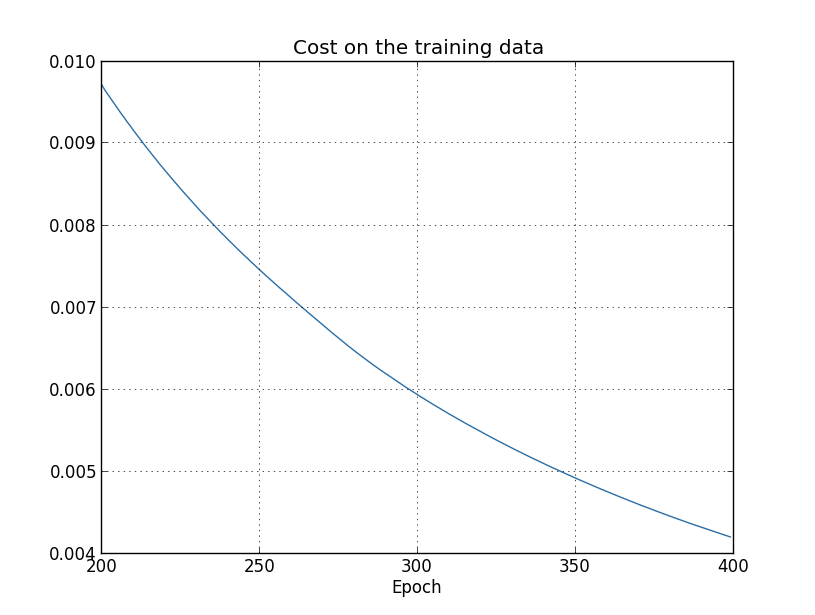
\includegraphics[width=0.867\textwidth]{images/overfitting1.png}
\end{center}

\noindent 这看起来令人鼓舞，显示出代价平滑下降，正如我们所预期的那样. 请注意，我只展示了第 200 到第 399 个训练轮次. 这让我们能够近距离地观察学习后期的阶段，而正如我们将看到的，有趣的事情恰恰发生在这里.

现在让我们看看测试数据上的分类准确率如何随时间变化：

\begin{center}
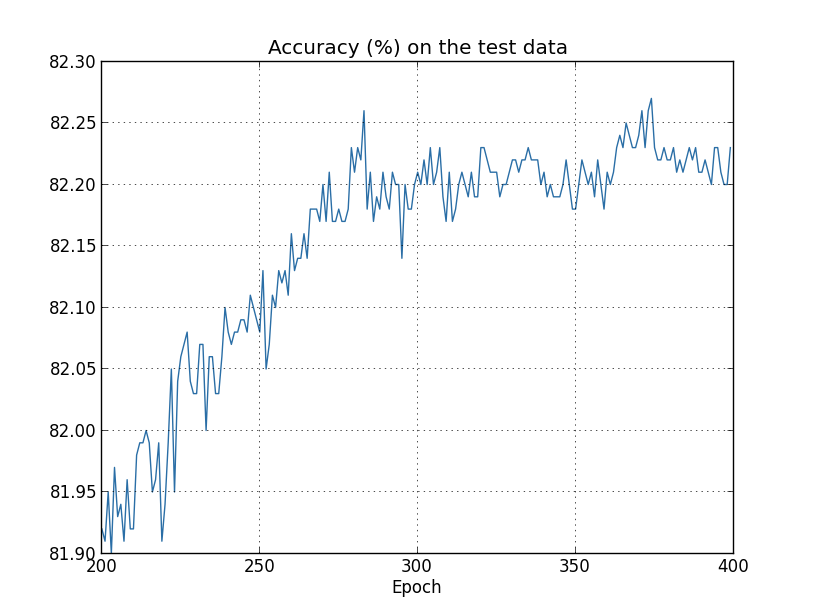
\includegraphics[width=0.867\textwidth]{images/overfitting2.png}
\end{center}

\noindent 同样，我做了相当程度的放大. 在前 200 个轮次（未显示）中，准确率上升到略低于 82\% 的水平. 然后学习逐渐放缓. 最后，在第 280 个轮次左右，分类准确率基本停止改善. 之后的轮次只是在第 280 个轮次的准确率值附近出现小的随机波动. 将此与之前的图对比，那里训练数据对应的代价仍在平滑下降. 如果我们只看那个代价，似乎我们的模型仍在变得``更好''. 但测试准确率的结果表明这种改善是一种错觉. 就像 Fermi 不喜欢的那个模型一样，我们的网络在第 280 个轮次之后学到的东西不再能泛化到测试数据. 因此这不是有用的学习. 我们说网络在第 280 个轮次之后发生了\emph{过拟合}或\emph{过度训练}.

你可能会想，这里的问题是不是我在看训练数据上的\emph{代价}，而不是测试数据上的\emph{分类准确率}. 换句话说，也许问题在于我们在做苹果和橘子的比较. 如果我们把训练数据上的代价与测试数据上的代价进行比较，也就是比较相似的度量，会怎样呢？或者我们可以比较训练数据和测试数据上的分类准确率？事实上，无论我们怎样比较，本质上都会出现同样的现象. 不过细节确实会有所不同. 例如，让我们看看测试数据上的代价：

\begin{center}
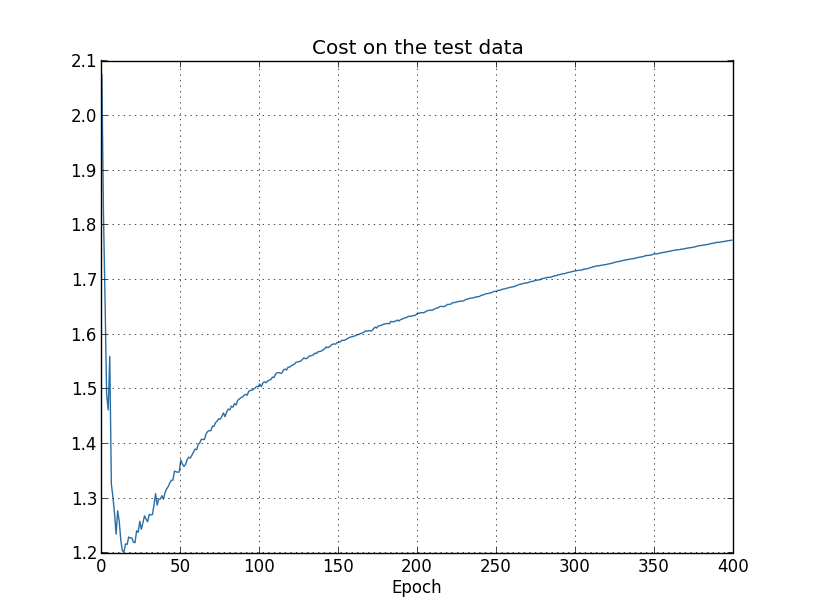
\includegraphics[width=0.867\textwidth]{images/overfitting3.png}
\end{center}

\noindent 我们可以看到，测试数据上的代价在第 15 个轮次左右之前一直在改善，但之后实际上开始变差，尽管训练数据上的代价仍在继续改善. 这是我们的模型正在过拟合\label{term:54}的另一个迹象. 不过，这提出了一个难题：我们应该把第 15 个轮次还是第 280 个轮次视为过拟合开始主导学习的节点？从实践的角度来看，我们真正关心的是提高测试数据上的分类准确率，而测试数据上的代价不过是分类准确率的一个代理指标. 因此，把第 280 个轮次视为我们的神经网络中过拟合开始主导学习的节点是最合理的.

过拟合的另一个迹象可以在训练数据上的分类准确率中看到：

\begin{center}
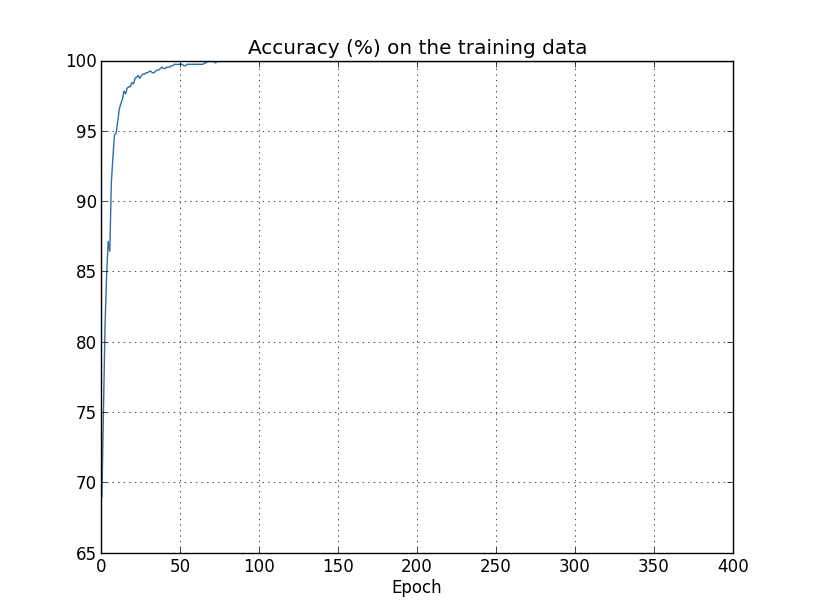
\includegraphics[width=0.867\textwidth]{images/overfitting4.png}
\end{center}

\noindent 准确率一路上升到 $100$\%. 也就是说，我们的网络正确地分类了全部 $1,000$ 张训练图像！与此同时，我们的测试准确率最高只有 $82.27$\% . 所以我们的网络确实是在学习训练集的特殊性，而不仅仅是在一般意义上识别数字. 几乎可以说，我们的网络只是在记忆训练集，而没有充分理解数字以便泛化到测试集\label{term:55}.

过拟合是神经网络中的一个主要问题. 在现代网络中尤其如此，因为这些网络通常拥有非常大量的权重和偏置. 为了有效地训练，我们需要一种检测过拟合何时发生的方法，这样我们就不会过度训练. 我们还希望有减少过拟合影响的技术.

检测过拟合的显而易见的方法是使用上面的做法，在网络训练过程中跟踪测试数据上的准确率. 如果我们看到测试数据上的准确率不再改善，就应该停止训练. 当然，严格来说，这并不一定是过拟合的迹象. 也可能是测试数据和训练数据上的准确率同时停止改善. 尽管如此，采用这一策略可以防止过拟合.

事实上，我们将使用这一策略的一个变体. 回想一下，当我们加载 MNIST 数据时，我们加载了三个数据集：

\begin{lstlisting}

>>> import mnist_loader
>>> training_data, validation_data, test_data = \
... mnist_loader.load_data_wrapper()

\end{lstlisting}

到目前为止，我们一直在使用 training\_\allowbreak{}data 和 test\_\allowbreak{}data，而忽略了 validation\_\allowbreak{}data.validation\_\allowbreak{}data 包含 $10,000$ 张数字图像，这些图像不同于 MNIST 训练集中的 $50,000$ 张图像，也不同于 MNIST 测试集中的 $10,000$ 张图像. 我们将使用 validation\_\allowbreak{}data 而不是 test\_\allowbreak{}data 来防止过拟合. 为此，我们将使用与上面针对 test\_\allowbreak{}data 所描述的几乎相同的策略. 也就是说，我们将在每个轮次结束时计算 validation\_\allowbreak{}data 上的分类准确率. 一旦 validation\_\allowbreak{}data 上的分类准确率饱和，我们就停止训练. 这一策略被称为提前停止\label{term:56}. 当然，在实践中我们不会立即知道准确率何时饱和. 相反，我们会继续训练，直到我们确信准确率已经饱和* *判断何时停止需要一些判断力. 在我之前的图中，我把第 280 个轮次确定为准确率饱和的位置. 这可能过于悲观了. 神经网络在训练中有时会停滞一段时间，然后继续改善. 如果更多的学习能在第 400 个轮次之后仍然发生，我也不会感到惊讶，尽管任何进一步改善的幅度可能很小. 因此，可以采用或多或少激进的提前停止策略..

为什么要使用 \texttt{validation\_\allowbreak{}data} 而不是 \texttt{test\_\allowbreak{}data} 来防止过拟合？事实上，这是一个更一般策略的一部分，即使用 \texttt{validation\_\allowbreak{}data} 来评估超参数的不同试验选择，例如训练的轮次数、学习率、最佳网络结构等等. 我们使用这样的评估来找到并设定超参数的良好值. 确实，尽管我直到现在才提到，但这在一定程度上就是我在本书前面做出超参数选择的方式.（稍后会详细讨论.）

当然，这丝毫没有回答为什么我们使用 \texttt{validation\_\allowbreak{}data} 而不是 \texttt{test\_\allowbreak{}data} 来防止过拟合的问题. 相反，它把这个问题替换成了一个更一般的问题：为什么我们使用 \texttt{validation\_\allowbreak{}data} 而不是 \texttt{test\_\allowbreak{}data} 来设定良好的超参数？要理解原因，请考虑在设定超参数时，我们很可能会尝试许多不同的超参数选择. 如果我们基于对 \texttt{test\_\allowbreak{}data} 的评估来设定超参数，就有可能最终把超参数过拟合到 \texttt{test\_\allowbreak{}data} 上. 也就是说，我们可能最终找到的超参数拟合了 \texttt{test\_\allowbreak{}data} 的特定特殊性，但网络的性能无法泛化到其他数据集. 我们通过使用 \texttt{validation\_\allowbreak{}data} 来确定超参数来防范这一点. 然后，一旦我们得到了想要的超参数，我们就使用 \texttt{test\_\allowbreak{}data} 做最终的准确率评估. 这让我们确信，我们在 \texttt{test\_\allowbreak{}data} 上的结果是我们的神经网络泛化能力的真实度量. 换一种说法，你可以把验证数据看作一种训练数据，它帮助我们学习良好的超参数. 这种寻找良好超参数的方法有时被称为\emph{留出}法，因为 \texttt{validation\_\allowbreak{}data} 被分离出来或``留出''于 \texttt{training\_\allowbreak{}data}.

现在，在实践中，即使在 \texttt{test\_\allowbreak{}data} 上评估了性能之后，我们也可能改变主意，想要尝试另一种方法——也许是不同的网络结构——这将涉及找到一组新的超参数. 如果我们这样做，难道不存在最终也会对 \texttt{test\_\allowbreak{}data} 过拟合的危险吗？我们是否需要潜在无限回归的数据集，才能确信我们的结果会泛化？完全解决这一顾虑是一个深刻而困难的问题. 但就我们的实际目的而言，我们不会过多担心这个问题. 相反，我们将继续前进，使用基本的留出法，基于 \texttt{training\_\allowbreak{}data}、\texttt{validation\_\allowbreak{}data} 和 \texttt{test\_\allowbreak{}data}，如上所述.

到目前为止，我们一直在看只使用 1,000 张训练图像时的过拟合. 当我们使用完整的 50,000 张图像训练集时会发生什么？我们将保持所有其他参数不变（30 个隐藏神经元、学习率 0.5、小批量大小 10），但使用全部 50,000 张图像训练 30 个轮次. 下面这张图展示了训练数据和测试数据上分类准确率的结果. 请注意，我在这里使用了测试数据而不是验证数据，以便使结果与之前的图更直接地可比.

\begin{center}
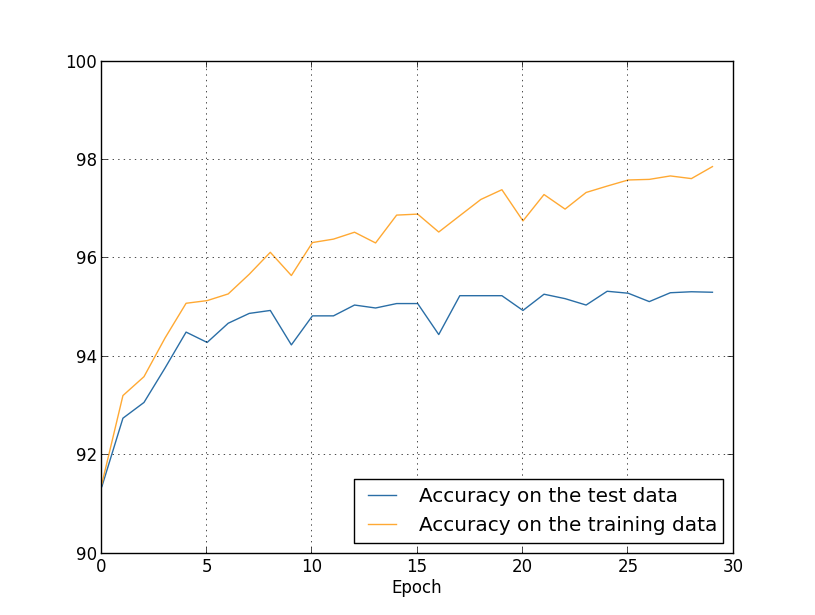
\includegraphics[width=0.867\textwidth]{images/overfitting_full.png}
\end{center}

如你所见，测试数据和训练数据上的准确率比我们使用 1,000 个训练样本时保持得更加接近. 特别是，训练数据上最好的分类准确率 $97.86$\% 仅比测试数据上的 $95.33$\% 高出 $2.53$\% . 这与我们之前 $17.73$\% 的差距相比！过拟合仍在发生，但已经大大减少了. 我们的网络从训练数据到测试数据的泛化能力好多了. 一般来说，减少过拟合的最佳方法之一就是增加训练数据的大小. 有了足够的训练数据，即使是非常大的网络也很难过拟合. 不幸的是，训练数据可能很昂贵或难以获取，所以这并不总是一个实际的选择.
\subsectionTitle{正则化}{正则化}

增加训练数据量是减少过拟合的一种方法. 我们还有其他方法可以减少过拟合的程度吗？一种可能的方法是缩小网络的规模. 然而，大型网络有可能比小型网络更强大，因此我们只会不情愿地采用这个选项.

幸运的是，还有其他技术可以减少过拟合，即使我们拥有固定的网络和固定的训练数据. 这些技术被称为\emph{正则化}技术. 在本节中，我将描述最常用的正则化技术之一，这种技术有时被称为\emph{权重衰减}或\emph{L2 正则化}. L2 正则化的思想是在代价函数中添加一个额外的项，这个项被称为\emph{正则化项}. 下面是正则化的交叉熵：

\begin{equation}
C = -\frac{1}{n} \sum_{xj} \left[ y_j \ln a^L_j+(1-y_j) \ln (1-a^L_j)\right] + \frac{\lambda}{2n} \sum_w w^2.
\tag{85}
\end{equation}

\noindent 第一项就是交叉熵的通常表达式. 但我们添加了第二项，即网络中所有\emph{权重}的平方和. 它被一个因子 $\lambda / 2n$ 缩放，其中 $\lambda > 0$ 被称为\emph{正则化参数}，而 $n$ 一如既往地是我们训练集的大小. 我稍后会讨论如何选择 $\lambda$. 同样值得注意的是，正则化项\emph{不}包含偏置. 我下面也会回到这一点.

当然，也可以对其他代价函数进行正则化，例如二次代价. 这可以用类似的方式完成：

\begin{equation}
C = \frac{1}{2n} \sum_x \|y-a^L\|^2 + \frac{\lambda}{2n} \sum_w w^2.
\tag{86}
\end{equation}

\noindent 在这两种情况下，我们可以将正则化的代价函数写为

\begin{equation}
C = C_0 + \frac{\lambda}{2n} \sum_w w^2,
\tag{87}
\end{equation}

\noindent 其中 $C_0$ 是原始的、未正则化的代价函数.

直观地说，正则化的效果是使网络在其他条件相同的情况下倾向于学习较小的权重. 只有当较大的权重能显著改善代价函数的第一部分时，它们才会被允许. 换句话说，正则化可以被视为在寻找小权重和最小化原始代价函数之间的一种折衷方式. 折衷中两个元素的相对重要性取决于 $\lambda$ 的值：当 $\lambda$ 很小时，我们倾向于最小化原始代价函数，但当 $\lambda$ 很大时，我们倾向于较小的权重.

现在，为什么做出这种折衷应该有助于减少过拟合，这一点其实一点也不明显！但事实证明它确实有帮助. 我们将在下一节中讨论它为什么有帮助的问题. 但首先，让我们通过一个例子来展示正则化确实能减少过拟合.

为了构造这样一个例子，我们首先需要弄清楚如何在正则化的神经网络中应用我们的随机梯度下降学习算法. 特别地，我们需要知道如何计算网络中所有权重和偏置的偏导数 $\partial C / \partial w$ 和 $\partial C / \partial b$. 对公式 (87) 求偏导数

\begin{align*}
C = C_0 + \frac{\lambda}{2n} \sum_w w^2 \nonumber
\end{align*}

\noindent 得到

\begin{align}
\frac{\partial C}{\partial w} &= \frac{\partial C_0}{\partial w} + \frac{\lambda}{n} w \tag{88} \\ \frac{\partial C}{\partial b} &= \frac{\partial C_0}{\partial b}. \tag{89}
\end{align}

\noindent $\partial C_0 / \partial w$ 和 $\partial C_0 / \partial b$ 项可以使用反向传播来计算，如上一章所述. 因此我们看到，计算正则化代价函数的梯度很容易：像往常一样使用反向传播，然后在所有\emph{权重}项的偏导数上加上 $\frac{\lambda}{n} w$. 关于偏置的偏导数保持不变，因此偏置的梯度下降学习规则与通常的规则相同：

\begin{equation}
b \rightarrow b -\eta \frac{\partial C_0}{\partial b}.
\tag{90}
\end{equation}

\noindent 权重的学习规则变为：

\begin{align}
w &\rightarrow w-\eta \frac{\partial C_0}{\partial w}-\frac{\eta \lambda}{n} w \tag{91} \\ &= \left(1-\frac{\eta \lambda}{n}\right) w -\eta \frac{\partial C_0}{\partial w}. \tag{92}
\end{align}

\noindent 这与通常的梯度下降学习规则完全相同，只是我们首先将权重 $w$ 乘以一个因子 $1-\frac{\eta \lambda}{n}$ 进行缩放. 这种缩放有时被称为\emph{权重衰减}，因为它使权重变小. 乍一看，这似乎意味着权重被不可阻挡地推向零. 但这是不对的，因为如果这样做能导致未正则化的代价函数减小，另一项可能会导致权重增加.

好了，这就是梯度下降的工作原理. 那随机梯度下降呢？嗯，就像在未正则化的随机梯度下降中一样，我们可以通过对 $m$ 个训练样本的小批量进行平均来估计 $\partial C_0 / \partial w$. 因此，随机梯度下降的正则化学习规则变为（参见公式 (20)

\begin{align*}
w_k &\rightarrow w_k' = w_k-\frac{\eta}{m} \sum_j \frac{\partial C_{X_j}}{\partial w_k} \nonumber
\end{align*}

\noindent ）

\begin{equation}
w \rightarrow \left(1-\frac{\eta \lambda}{n}\right) w -\frac{\eta}{m} \sum_x \frac{\partial C_x}{\partial w},
\tag{93}
\end{equation}

\noindent 其中求和是对小批量中的训练样本 $x$ 进行的，而 $C_x$ 是每个训练样本的（未正则化的）代价. 这与随机梯度下降的通常规则完全相同，除了 $1-\frac{\eta \lambda}{n}$ 权重衰减\label{term:57}因子. 最后，为了完整起见，让我陈述一下偏置的正则化学习规则. 当然，这与未正则化的情况完全相同（参见公式 (21)

\begin{align*}
b_l &\rightarrow b_l' = b_l-\frac{\eta}{m} \sum_j \frac{\partial C_{X_j}}{\partial b_l} \nonumber
\end{align*}

\noindent ），

\begin{equation}
b \rightarrow b - \frac{\eta}{m} \sum_x \frac{\partial C_x}{\partial b},
\tag{94}
\end{equation}

\noindent 其中求和是对小批量中的训练样本 $x$ 进行的.

让我们看看正则化如何改变我们神经网络的性能. 我们将使用一个有 $30$ 个隐藏神经元的网络，小批量大小为 $10$，学习率为 $0.5$，并使用交叉熵代价函数. 然而，这次我们将使用 $\lambda = 0.1$ 的正则化参数. 注意，在代码中，我们使用变量名 \texttt{lmbda}，因为 \texttt{lambda} 是 Python 中的保留字，含义与此无关. 我还再次使用了 \texttt{test\_\allowbreak{}data}，而不是 \texttt{validation\_\allowbreak{}data}. 严格来说，出于我们之前讨论过的所有原因，我们应该使用 \texttt{validation\_\allowbreak{}data}. 但我决定使用 \texttt{test\_\allowbreak{}data}，因为它使结果与我们之前未正则化的结果更直接可比. 你可以轻松地将代码改为使用 \texttt{validation\_\allowbreak{}data}，你会发现它给出了类似的结果.

\begin{lstlisting}

>>> import mnist_loader
>>> training_data, validation_data, test_data = \
... mnist_loader.load_data_wrapper()
>>> import network2
>>> net = network2.Network([784, 30, 10], cost=network2.CrossEntropyCost)
>>> net.large_weight_initializer()
>>> net.SGD(training_data[:1000], 400, 10, 0.5,
... evaluation_data=test_data, lmbda = 0.1,
... monitor_evaluation_cost=True, monitor_evaluation_accuracy=True,
... monitor_training_cost=True, monitor_training_accuracy=True)

\end{lstlisting}

训练数据上的代价在整个过程中都在下降，与之前未正则化的情况非常相似* *这个图和接下来两个图是用程序 overfitting.py 生成的.：

\begin{center}
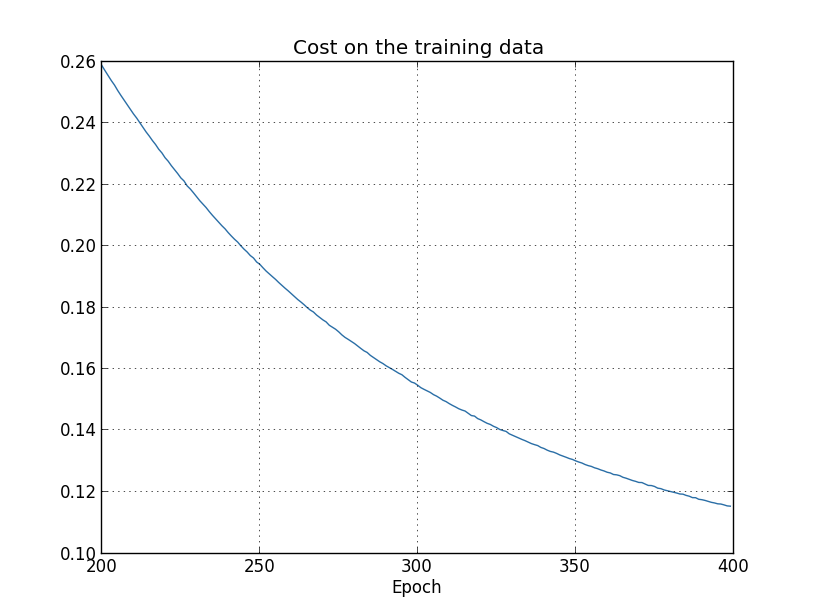
\includegraphics[width=0.867\textwidth]{images/regularized1.png}
\end{center}

\noindent 但这次 \texttt{test\_\allowbreak{}data} 上的准确率在整个 400 个轮次中持续增加：

\begin{center}
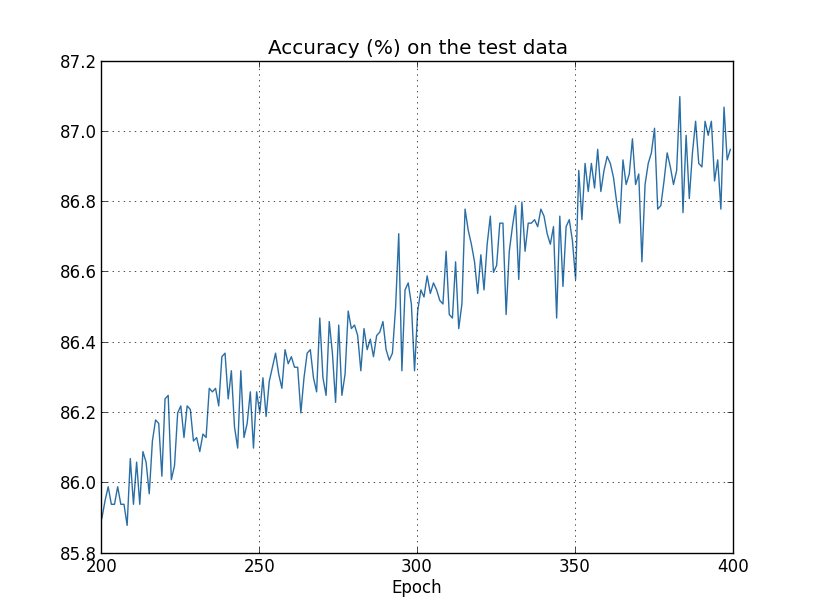
\includegraphics[width=0.867\textwidth]{images/regularized2.png}
\end{center}

\noindent 显然，正则化的使用抑制了过拟合. 更重要的是，准确率显著提高，峰值分类准确率为 $87.1$ 百分比，而未正则化情况下获得的峰值为 $82.27$ 百分比. 事实上，通过继续训练超过 400 个轮次，我们几乎肯定可以获得相当好的结果. 从经验上看，正则化似乎使我们的网络泛化得更好，并显著减少了过拟合的影响.

如果我们走出只有 1,000 张训练图像的人为环境，回到完整的 50,000 张图像训练集，会发生什么？当然，我们已经看到，在完整的 50,000 张图像下，过拟合问题要小得多. 正则化还有进一步的帮助吗？让我们保持超参数与之前相同——$30$ 个轮次，学习率 $0.5$，小批量大小为 $10$. 然而，我们需要修改正则化参数. 原因是训练集的大小 $n$ 从 $n = 1,000$ 变为 $n = 50,000$，这改变了权重衰减因子 $1 - \frac{\eta \lambda}{n}$. 如果我们继续使用 $\lambda = 0.1$，那将意味着权重衰减少得多，因此正则化效果也小得多. 我们通过改为 $\lambda = 5.0$ 来补偿.

好了，让我们训练我们的网络，首先停下来重新初始化权重：

\begin{lstlisting}

>>> net.large_weight_initializer()
>>> net.SGD(training_data, 30, 10, 0.5,
... evaluation_data=test_data, lmbda = 5.0,
... monitor_evaluation_accuracy=True, monitor_training_accuracy=True)

\end{lstlisting}

我们得到结果：

\begin{center}
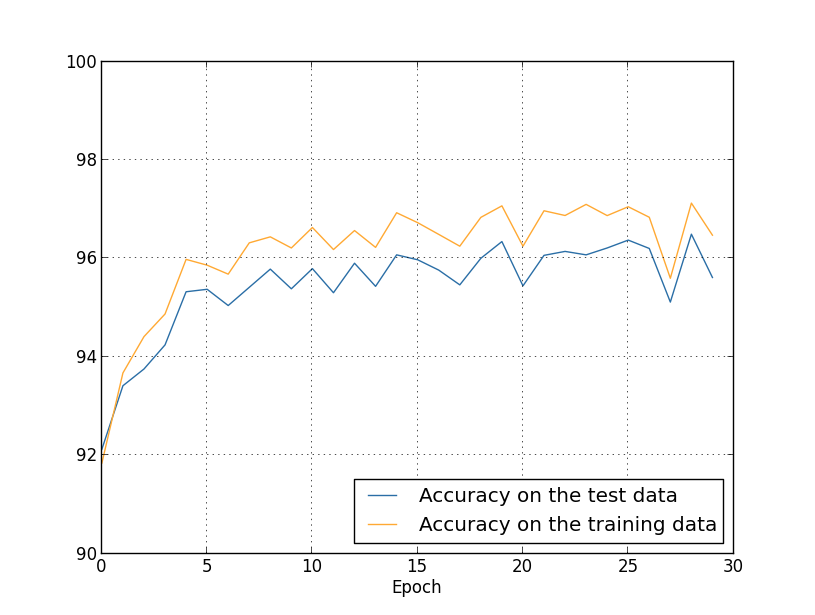
\includegraphics[width=0.867\textwidth]{images/regularized_full.png}
\end{center}

\noindent 这里有很多好消息. 首先，我们在测试数据上的分类准确率提高了，从未正则化时的 $95.49$ 百分比提高到 $96.49$ 百分比. 这是一个很大的改进. 其次，我们可以看到训练数据和测试数据上的结果之间的差距比以前小得多，不到一个百分点. 这仍然是一个显著的差距，但我们显然在减少过拟合方面取得了实质性进展.

最后，让我们看看当我们使用 100 个隐藏神经元和正则化参数 $\lambda = 5.0$ 时，测试分类准确率是多少. 我不会在这里详细分析过拟合，这纯粹是为了好玩，只是为了看看当我们使用我们的新技巧：交叉熵代价函数和 L2 正则化时，我们能获得多高的准确率.

\begin{lstlisting}

>>> net = network2.Network([784, 100, 10], cost=network2.CrossEntropyCost)
>>> net.large_weight_initializer()
>>> net.SGD(training_data, 30, 10, 0.5, lmbda=5.0,
... evaluation_data=validation_data,
... monitor_evaluation_accuracy=True)

\end{lstlisting}

最终结果是在验证数据上的分类准确率为 $97.92$ 百分比. 这比 30 个隐藏神经元的情况有了很大的飞跃. 事实上，只需再稍微调整一下，以 $\eta = 0.1$ 和 $\lambda = 5.0$ 运行 60 个轮次，我们就突破了 $98$ 百分比的障碍，在验证数据上达到了 $98.04$ 百分比的分类准确率. 对于最终只有 152 行代码的程序来说，这还不错！

我将正则化描述为一种减少过拟合和提高分类准确率的方法. 事实上，这并不是唯一的好处. 根据经验，当对我们的 MNIST 网络进行多次运行，但使用不同的（随机）权重初始化时，我发现未正则化的运行偶尔会``卡住''，显然陷入了代价函数的局部极小值. 结果是不同的运行有时会提供相当不同的结果. 相比之下，正则化的运行提供了更容易复现的结果.

为什么会这样？启发式地说，如果代价函数未正则化，那么在其他条件相同的情况下，权重向量的长度很可能会增长. 随着时间的推移，这可能导致权重向量变得非常大. 这可能导致权重向量卡在指向大致相同的方向上，因为当长度很长时，梯度下降引起的变化只会对方向产生微小的改变. 我相信这种现象使我们的学习算法难以正确地探索权重空间，从而更难找到代价函数的良好极小值.
\subsectionTitle{正则化为何能减轻过拟合？}{正则化为何能减轻过拟合？}

我们已经从经验上看到，正则化有助于减轻过拟合. 这令人鼓舞，但不幸的是，正则化为什么有帮助却并不显然！人们用来解释所发生之事的一个标准说法大致如下：更小的权重在某种意义上意味着更低的复杂度，因此为数据提供了一个更简单也更有力的解释，因而应当被偏好. 不过，这是一个相当简略的说法，其中包含若干也许显得可疑或令人费解的成分. 让我们把这个说法拆解开来并批判性地加以审视. 为此，让我们假设有一个简单的数据集，我们希望为其建立一个模型：这里隐含地，我们在研究某个现实世界的现象，其中 $x$ 和 $y$ 表示现实世界的数据. 我们的目标是建立一个模型，使我们能够把 $y$ 预测为 $x$ 的函数. 我们可以尝试用神经网络来建立这样一个模型，但我要做一件更简单的事：我将尝试把 $y$ 建模为 $x$ 的多项式. 我这样做而不是使用神经网络，是因为使用多项式会让事情变得特别透明. 一旦我们理解了多项式的情形，我们就会把它翻译到神经网络上. 现在，上图中有十个点，这意味着我们可以找到一个唯一的 $9$ 阶多项式 $y = a_0 x^9 + a_1 x^8 + \ldots + a_9$ 精确地拟合这些数据. 下面是该多项式的图像*\footnote{我不会显式地给出系数，尽管使用诸如 Numpy 的 \texttt{polyfit} 这样的例程很容易找到它们. 如果你好奇，可以在生成该图像的源代码中查看该多项式的确切形式. 它就是生成该图像的程序中从第 14 行开始定义的函数 \texttt{p(x)}.}：这提供了一个精确的拟合. 但我们也可以用一个线性模型 $y = 2x$ 得到很好的拟合：这两个模型中哪一个更好？哪一个更可能是真的？对于同一个潜在的现实世界现象的其他样本，哪一个模型更可能泛化得好？

这些都是困难的问题. 事实上，如果没有关于潜在现实世界现象的更多信息，我们无法确定地回答上述任何一个问题. 但让我们考虑两种可能性：(1) $9$ 阶多项式实际上就是真正描述该现实世界现象的模型，因此该模型将完美地泛化；(2) 正确的模型是 $y = 2x$，但存在一点额外的噪声，比如说由于测量误差，这就是为什么该模型不是精确拟合的原因.

\emph{先验地}，我们不可能说出这两种可能性中哪一种是对的. （或者，是否某个第三种可能性成立.）从逻辑上讲，两者都可能为真. 而且这并不是一个微不足道的差别. 诚然，在所提供的数据上，两个模型之间只有很小的差别. 但假设我们想要预测某个很大的 $x$ 值所对应的 $y$ 值，这个 $x$ 值远大于上图中所显示的任何值. 如果我们试图这样做，两个模型的预测之间将会出现巨大的差别，因为 $9$ 阶多项式模型会逐渐被 $x^9$ 项所主导，而线性模型则保持，嗯，线性.

一种观点是说，在科学中我们应当采用更简单的解释，除非被迫不这样做. 当我们发现一个似乎能解释许多数据点的简单模型时，我们会忍不住高呼``找到了！''. 毕竟，一个简单的解释仅仅出于巧合而出现，这似乎不太可能. 相反，我们怀疑该模型必定表达了关于该现象的某种潜在真理. 在手头这个情形中，模型 $y = 2x+{\rm noise}$ 似乎比 $y = a_0 x^9 + a_1 x^8 + \ldots$ 简单得多. 如果这种简单性是偶然出现的，那会令人惊讶，因此我们怀疑 $y = 2x+{\rm noise}$ 表达了某种潜在真理. 在这种观点下，9 阶模型实际上只是在学习局部噪声的影响. 因此，虽然 9 阶模型对这些特定的数据点完美有效，但该模型将无法泛化到其他数据点，而带噪声的线性模型将具有更强的预测能力.

让我们看看这种观点对神经网络意味着什么. 假设我们的网络大多具有较小的权重，这在正则化的网络中往往会如此. 权重之小意味着，如果我们在这里或那里改变几个随机输入，网络的行为不会变化太大. 这使得正则化的网络难以学习数据中局部噪声的影响. 可以把它看作一种使单个证据对网络输出不太重要的方式. 相反，正则化的网络学会对训练集中经常出现的证据类型作出响应. 相比之下，具有大权重的网络可能会因输入的微小变化而使其行为发生相当大的变化. 因此，未正则化的网络可以利用大权重来学习一个复杂的模型，该模型携带了大量关于训练数据中噪声的信息. 简而言之，正则化的网络被约束为基于训练数据中经常出现的模式来建立相对简单的模型，并且抗拒学习训练数据中噪声的奇特之处. 我们希望这将迫使我们的网络真正地学习手头现象，并从它们所学到的东西中更好地泛化.

话虽如此，这种偏好更简单解释的想法应当让你感到不安. 人们有时把这种想法称为``奥卡姆剃刀''，并会热切地应用它，仿佛它具有某种一般科学原理的地位. 但是，当然，它并不是一条一般科学原理. 并没有\emph{先验的}逻辑理由去偏好简单的解释而非更复杂的解释. 事实上，有时更复杂的解释结果才是正确的.

让我描述两个更复杂的解释结果被证明是正确的例子. 20 世纪 40 年代，物理学家 Marcel Schein 宣布发现了一种新的自然粒子. 他所在的公司通用电气欣喜若狂，并广泛宣传这一发现. 但物理学家 Hans Bethe 持怀疑态度. Bethe 拜访了 Schein，并查看了显示 Schein 新粒子径迹的底片. Schein 给 Bethe 看了一张又一张底片，但在每一张底片上 Bethe 都指出了某个问题，暗示这些数据应当被丢弃. 最后，Schein 给 Bethe 看了一张看起来不错的底片. Bethe 说这可能只是一个统计上的偶然. Schein：``是的，但即使按照你自己的公式，这是统计巧合的机会也只有五分之一.'' Bethe：``但我们已经看了五张底片了.'' 最后，Schein 说：``但在我的底片上，每一张好的底片，每一张好的照片，你都用不同的理论来解释，而我有一个假设能解释所有底片，即它们是[新粒子].'' Bethe 回答说：``你的解释和我的解释之间唯一的区别是，你的解释是错的，而我的所有解释都是对的. 你那个单一的解释是错的，而我那些多个解释都是对的.'' 随后的工作证实，大自然同意 Bethe 的看法，Schein 的粒子不复存在*\footnote{这个故事由物理学家 Richard Feynman 在接受历史学家 Charles Weiner 采访时讲述.}.

作为第二个例子，1859 年，天文学家 Urbain Le Verrier 观察到水星轨道的形状与牛顿引力理论所说的并不完全一致. 这是对牛顿理论一个极其微小的偏离，当时提出的若干解释归结起来都是说牛顿理论或多或少是对的，但需要一点微小的修改. 1916 年，Einstein 表明，这个偏离可以用他的广义相对论很好地解释，这是一个与牛顿引力截然不同的理论，建立在复杂得多的数学之上. 尽管有这种额外的复杂性，今天人们已经接受 Einstein 的解释是正确的，而牛顿引力，即使在其修改形式下，也是错的. 这在一定程度上是因为我们现在知道 Einstein 的理论解释了许多牛顿理论难以处理的其它现象. 此外，甚至更令人印象深刻的是，Einstein 的理论准确地预言了若干牛顿引力根本没有预言的现象. 但这些令人印象深刻的品质在早期并不完全明显. 如果仅仅根据简单性来判断，那么牛顿理论的某种修改形式可以说会更有吸引力.

从这些故事中可以得出三点教益. 第一，判断两种解释中哪一种真正``更简单''可能是一件相当微妙的事情. 第二，即使我们能够做出这样的判断，简单性也是一条必须极其谨慎使用的指南！第三，对一个模型的真正检验不是简单性，而是它在新的行为区域中预测新现象的表现有多好.

话虽如此，并且牢记需要谨慎，正则化的神经网络通常比未正则化的网络泛化得更好，这是一个经验事实. 因此，在本书余下的部分中，我们将频繁使用正则化. 我之所以加入上面的故事，仅仅是为了帮助传达为什么还没有人发展出一个完全令人信服的理论解释，来说明正则化为何有助于网络泛化. 事实上，研究者们继续撰写论文，在论文中他们尝试不同的正则化方法，比较它们以看哪一种效果更好，并试图理解为什么不同的方法效果更好或更差. 因此你可以把正则化看作某种拼凑之物. 虽然它常常有帮助，但我们并没有一个完全令人满意的系统性理解来说明究竟发生了什么，只有不完整的启发式方法和经验法则.

这里还有一组更深层的问题，这些问题触及科学的本质. 这就是我们如何泛化的问题. 正则化也许给了我们一根计算上的魔杖，帮助我们的网络更好地泛化，但它并没有给我们一个关于泛化如何运作的原则性理解，也没有告诉我们最好的方法是什么*\footnote{这些问题可以追溯到归纳问题，苏格兰哲学家 David Hume 在``An Enquiry Concerning Human Understanding''（1748）中对此有过著名讨论. 归纳问题在 David Wolpert 和 William Macready（1997）的无免费午餐定理（链接）中被赋予了现代机器学习的形态.}.

这尤其令人恼火，因为在日常生活中，我们人类的泛化能力好得惊人. 只要给一个孩子看几张大象的图片，他很快就会学会辨认其它大象. 当然，他们偶尔可能会犯错，也许会把犀牛误认为大象，但总的来说这个过程运作得极其准确. 所以我们有一个系统——人脑——拥有数量巨大的自由参数. 而在只被展示一张或少数几张训练图像之后，该系统就学会了泛化到其它图像. 在某种意义上，我们的大脑正则化得非常好！我们是如何做到这一点的？在这一点上我们并不知道. 我预计在未来的岁月里，我们将发展出更强大的技术来对人工神经网络进行正则化，这些技术最终将使神经网络即使从小数据集也能很好地泛化.

事实上，我们的网络已经比人们\emph{先验地}所期望的泛化得更好. 一个有 100 个隐藏神经元的网络有近 80,000 个参数. 我们的训练数据中只有 50,000 张图像. 这就像试图用一个 80,000 阶多项式去拟合 50,000 个数据点. 按理说，我们的网络应当严重过拟合. 然而，正如我们之前所看到的，这样一个网络实际上泛化得相当不错. 为什么会这样？这一点还没有被很好地理解. 有人猜测*\footnote{在 Gradient-Based Learning Applied to Document Recognition 中，作者为 Yann LeCun、Léon Bottou、Yoshua Bengio 和 Patrick Haffner（1998）.}``多层网络中梯度下降学习的动力学具有一种`自正则化'效应''. 这是格外幸运的，但我们不理解为什么会这样，这也有些令人不安. 与此同时，我们将采取务实的做法，只要能够就使用正则化. 我们的神经网络将因此变得更好.

让我通过回到一个我早先未加解释的细节来结束本节：L2 正则化\emph{并不}约束偏置这一事实. 当然，修改正则化过程以对偏置进行正则化是很容易的. 从经验上看，这样做通常不会使结果发生太大变化，所以在某种程度上，是否对偏置进行正则化只是一个约定. 然而，值得注意的是，拥有一个大的偏置并不会像拥有大的权重那样使一个神经元对其输入敏感. 因此我们不必担心大的偏置会使我们的网络学习训练数据中的噪声. 与此同时，允许大的偏置使我们的网络在行为上具有更大的灵活性——特别是，大的偏置使神经元更容易饱和，而这有时是可取的. 由于这些原因，我们在正则化时通常不包含偏置项.
\subsectionTitle{正则化的其他技术}{正则化的其他技术}

除了 L2 正则化之外，还有许多正则化技术. 事实上，已经发展出了如此多的技术，我无法将它们全部总结出来. 在本节中，我简要描述另外三种减少过拟合的方法：L1 正则化、dropout，以及人为地增大训练集规模. 我们不会像之前那样深入地研究这些技术. 相反，目的是熟悉主要思想，并体会一下可用的正则化技术的多样性. \textbf{L1 正则化：} 在这种方法中，我们通过加上权重绝对值之和来修改未正则化的代价函数：

\begin{equation}
C = C_0 + \frac{\lambda}{n} \sum_w |w|.
\tag{95}
\end{equation}

\noindent 直观上，这与 L2 正则化类似，惩罚大的权重，并倾向于让网络偏好小的权重. 当然，L1 正则化项与 L2 正则化项并不相同，因此我们不应期望得到完全相同的行为. 让我们试着理解用 L1 正则化训练的网络的行为与用 L2 正则化训练的网络有何不同.

为此，我们来看代价函数的偏导数. 对 (95) 求导

\begin{align*}
C = C_0 + \frac{\lambda}{n} \sum_w |w| \nonumber
\end{align*}

\noindent 我们得到：

\begin{equation}
\frac{\partial C}{\partial w} = \frac{\partial C_0}{\partial w} + \frac{\lambda}{n} \, {\rm sgn}(w),
\tag{96}
\end{equation}

\noindent 其中 ${\rm sgn}(w)$ 是 $w$ 的符号，也就是说，如果 $w$ 为正则为 $+1$，如果 $w$ 为负则为 $-1$. 利用这个表达式，我们可以很容易地修改反向传播，以使用 L1 正则化进行随机梯度下降. 对于 L1 正则化的网络，得到的更新规则是

\begin{equation}
w \rightarrow w' = w-\frac{\eta \lambda}{n} \mbox{sgn}(w) - \eta \frac{\partial C_0}{\partial w},
\tag{97}
\end{equation}

\noindent 其中，和通常一样，如果需要的话，我们可以用小批量平均来估计 $\partial C_0 / \partial w$. 将其与 L2 正则化的更新规则（参见方程 (93)

\begin{align*}
w \rightarrow \left(1-\frac{\eta \lambda}{n}\right) w -\frac{\eta}{m} \sum_x \frac{\partial C_x}{\partial w}, \nonumber
\end{align*}

\noindent ）相比较，

\begin{equation}
w \rightarrow w' = w\left(1 - \frac{\eta \lambda}{n} \right) - \eta \frac{\partial C_0}{\partial w}.
\tag{98}
\end{equation}

\noindent 在这两个表达式中，正则化的效果都是收缩权重. 这与我们的直觉一致，即两种正则化都惩罚大的权重. 但权重收缩的方式不同. 在 L1 正则化中，权重以恒定的量向 $0$ 收缩. 在 L2 正则化中，权重收缩的量与 $w$ 成正比. 因此，当某个权重的绝对值 $|w|$ 很大时，L1 正则化对该权重的收缩远小于 L2 正则化. 相反，当 $|w|$ 很小时，L1 正则化对该权重的收缩远大于 L2 正则化. 最终结果是，L1 正则化倾向于将网络的权重集中在相对少数几个高重要性的连接上，而其他权重则被驱向零.

我在上面的讨论中回避了一个问题，即当 $w = 0$ 时偏导数 $\partial C / \partial w$ 没有定义. 原因是函数 $|w|$ 在 $w = 0$ 处有一个尖锐的``角''，因此在该点不可微. 不过没关系. 我们要做的只是在 $w = 0$ 时应用通常的（未正则化的）随机梯度下降规则. 这应该没问题——直观上，正则化的效果是收缩权重，而显然它无法收缩一个已经是 $0$ 的权重. 更确切地说，我们将使用方程 (96)

\begin{align*}
\frac{\partial C}{\partial w} = \frac{\partial C_0}{\partial w} + \frac{\lambda}{n} \, {\rm sgn}(w) \nonumber
\end{align*}

\noindent 和 (97)

\begin{align*}
w \rightarrow w' = w-\frac{\eta \lambda}{n} \mbox{sgn}(w) - \eta \frac{\partial C_0}{\partial w} \nonumber
\end{align*}

\noindent 并约定 $\mbox{sgn}(0) = 0$. 这就给出了一个简洁的规则，用于在 L1 正则化下进行随机梯度下降. \textbf{Dropout：} Dropout 是一种截然不同的正则化技术. 与 L1 和 L2 正则化不同，dropout 不依赖于修改代价函数. 相反，在 dropout 中我们修改网络本身. 让我先描述 dropout 工作的基本机制，然后再讨论它为什么有效，以及结果如何.

假设我们试图训练一个网络：

\begin{center}
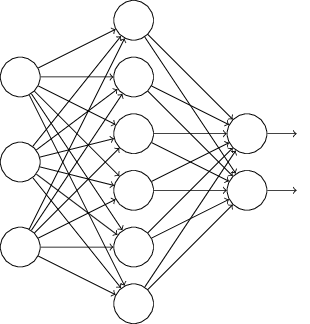
\includegraphics[width=0.9\textwidth]{images/tikz30.png}
\end{center}

\noindent 特别地，假设我们有一个训练输入 $x$ 和对应的期望输出 $y$. 通常，我们会通过将 $x$ 前馈传播通过网络来训练，然后反向传播以确定对梯度的贡献. 使用 dropout 时，这个过程被修改了. 我们首先随机地（并且暂时地）删除网络中一半的隐藏神经元，同时保持输入和输出神经元不变. 这样做之后，我们将得到一个大致如下的网络. 注意，被 dropout 的神经元，即那些被暂时删除的神经元，仍然以虚影显示：

\begin{center}
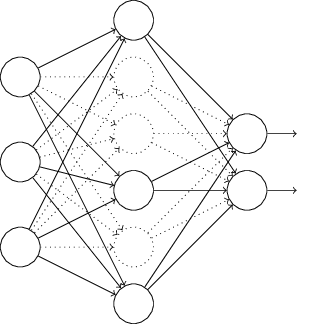
\includegraphics[width=0.9\textwidth]{images/tikz31.png}
\end{center}

\noindent 我们将输入 $x$ 通过修改后的网络前馈传播，然后将结果也通过修改后的网络反向传播. 在一个小批量的样本上这样做之后，我们更新相应的权重和偏置. 然后我们重复这个过程，首先恢复被 dropout 的神经元，然后选择一个新的随机隐藏神经元子集来删除，为另一个小批量估计梯度，并更新网络中的权重和偏置.

通过一遍又一遍地重复这个过程，我们的网络将学到一组权重和偏置. 当然，这些权重和偏置是在一半隐藏神经元被丢弃的条件下学到的. 当我们实际运行完整的网络时，这意味着将有两倍的隐藏神经元处于活跃状态. 为了补偿这一点，我们将从隐藏神经元输出的权重减半.

这个 dropout 过程可能看起来奇怪且\emph{临时拼凑}. 我们为什么会期望它有助于正则化呢？为了解释这是怎么回事，我希望你暂时停止思考 dropout，而是想象以标准方式（无 dropout）训练神经网络. 特别地，想象我们训练几个不同的神经网络，都使用相同的训练数据. 当然，这些网络可能一开始并不完全相同，因此训练后它们有时可能给出不同的结果. 当这种情况发生时，我们可以使用某种平均或投票方案来决定接受哪个输出. 例如，如果我们训练了五个网络，其中三个将某个数字分类为``3''，那么它很可能真的是``3''. 另外两个网络很可能只是犯了错误. 这种平均方案通常被发现是一种强大（尽管昂贵）的减少过拟合的方法. 原因是不同的网络可能以不同的方式过拟合，而平均可能有助于消除那种过拟合.

这与 dropout 有什么关系呢？启发式地说，当我们 dropout 不同的神经元集合时，这有点像我们在训练不同的神经网络. 因此，dropout 过程就像是对大量不同网络的效果进行平均. 不同的网络会以不同的方式过拟合，因此，希望 dropout 的净效果是减少过拟合.

在一篇最早使用该技术的论文*\footnote{ImageNet Classification with Deep Convolutional Neural Networks, by Alex Krizhevsky, Ilya Sutskever, and Geoffrey Hinton (2012).}中给出了一个相关的启发式解释：``This technique reduces complex co-adaptations of neurons, since a neuron cannot rely on the presence of particular other neurons. It is, therefore, forced to learn more robust features that are useful in conjunction with many different random subsets of the other neurons.'' 换句话说，如果我们把网络看作一个正在做出预测的模型，那么我们可以把 dropout 看作一种确保模型对丢失任何单个证据片段都具有鲁棒性的方法. 在这一点上，它有点类似于 L1 和 L2 正则化，后者倾向于减小权重，从而使网络对丢失网络中的任何单个连接更加鲁棒.

当然，dropout 的真正衡量标准是它在提高神经网络性能方面非常成功. 引入该技术的原始论文*\footnote{Improving neural networks by preventing co-adaptation of feature detectors by Geoffrey Hinton, Nitish Srivastava, Alex Krizhevsky, Ilya Sutskever, and Ruslan Salakhutdinov (2012). Note that the paper discusses a number of subtleties that I have glossed over in this brief introduction.}将其应用于许多不同的任务. 对我们来说，特别感兴趣的是他们将 dropout 应用于 MNIST 数字分类，使用了一个类似于我们一直在考虑的那种普通前馈神经网络. 论文指出，在此之前，使用这种架构所取得的最佳结果是在测试集上达到 $98.4$ ％的分类准确率. 他们使用 dropout 和一种修改形式的 L2 正则化的组合，将其提高到 $98.7$ ％的准确率. 在许多其他任务上也获得了类似令人印象深刻的结果，包括图像和语音识别以及自然语言处理中的问题. Dropout 在训练大型深度网络时特别有用，因为在这些网络中过拟合问题往往很严重. \textbf{人为地扩展训练数据：} 我们之前看到，当我们只使用 1,000 张训练图像时，我们的 MNIST 分类准确率下降到 80 ％多. 这并不奇怪，因为更少的训练数据意味着我们的网络将接触到更少的人类书写数字方式的变化. 让我们尝试用各种不同的训练数据集大小来训练我们的 30 个隐藏神经元网络，看看性能如何变化. 我们使用小批量大小 10、学习率 $\eta = 0.5$、正则化参数 $\lambda = 5.0$ 以及交叉熵代价函数进行训练. 当使用完整训练数据集时，我们将训练 30 个轮次，当使用较小的训练集时，我们将按比例增加轮次数量. 为了确保权重衰减因子在不同训练集之间保持一致，当使用完整训练数据集时，我们将使用正则化参数 $\lambda = 5.0$，当使用较小的训练集时，我们将按比例减小 $\lambda$*\footnote{This and the next two graph are produced with the program more\_\allowbreak{}data.py.}.

\begin{center}
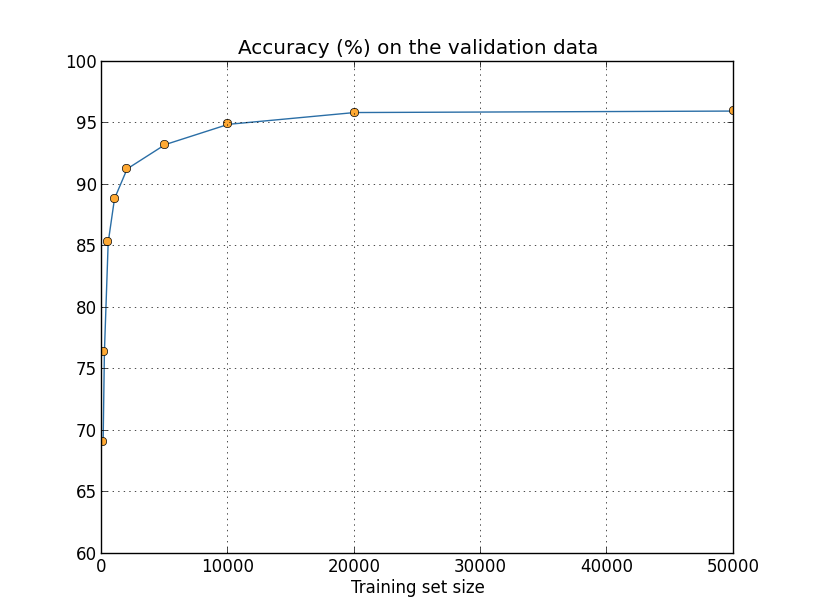
\includegraphics[width=0.867\textwidth]{images/more_data.png}
\end{center}

如你所见，随着我们使用更多的训练数据，分类准确率显著提高. 如果有更多数据可用，这种改进大概还会继续. 当然，看上面的图，确实看起来我们正在接近饱和. 然而，假设我们用对数坐标绘制训练集大小来重做这个图：

\begin{center}
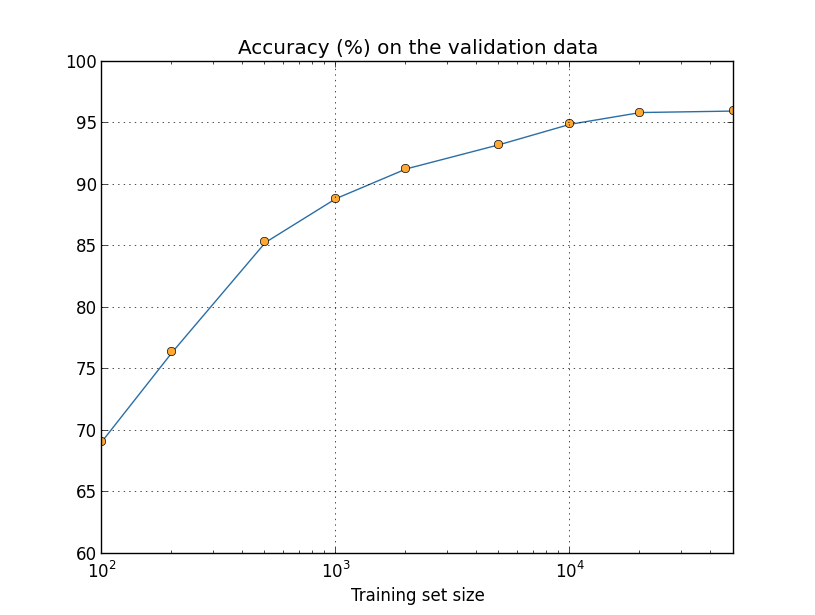
\includegraphics[width=0.867\textwidth]{images/more_data_log.png}
\end{center}

\noindent 很明显，图在末端仍在上升. 这表明，如果我们使用多得多的训练数据——比如说，数百万甚至数十亿个手写样本，而不仅仅是 50,000 个——那么我们很可能会获得相当好的性能，即使是从这个非常小的网络.

获取更多训练数据是个好主意. 不幸的是，这可能很昂贵，因此在实践中并不总是可行. 然而，还有另一个几乎同样有效的想法，那就是人为地扩展训练数据. 例如，假设我们取一张 MNIST 训练图像中的数字五，

\begin{center}

\includegraphics[width=0.200\textwidth]{images/more_data_5.png}
\end{center}

\noindent 并将其旋转一个小角度，比如说 15 度：

\begin{center}

\includegraphics[width=0.200\textwidth]{images/more_data_rotated_5.png}
\end{center}

\noindent 它仍然可以识别为同一个数字. 然而在像素层面上，它与 MNIST 训练数据中当前的任何图像都相当不同. 可以想象，将这张图像添加到训练数据中可能有助于我们的网络学习更多关于如何分类数字的知识. 更重要的是，显然我们不仅限于添加这一张图像. 我们可以通过对\emph{所有} MNIST 训练图像进行\emph{许多}小的旋转来扩展我们的训练数据，然后使用扩展后的训练数据来提高我们网络的性能.
这个想法非常强大，并且已被广泛使用. 让我们看一篇论文* \footnote{Best Practices for Convolutional Neural Networks Applied to Visual Document Analysis, by Patrice Simard, Dave Steinkraus, and John Platt (2003).} 中的一些结果，该论文将这个想法的几种变体应用于 MNIST. 他们考虑的其中一种神经网络架构与我们一直在使用的类似，是一个具有 800 个隐藏神经元并使用交叉熵代价函数的前馈网络. 使用标准的 MNIST 训练数据运行该网络，他们在测试集上达到了 98.4\% 的分类准确率. 但随后他们扩展了训练数据，不仅使用了如我上文所述的旋转，还使用了平移和倾斜图像. 通过在扩展数据集上训练，他们将网络的准确率提高到了 98.9\%. 他们还实验了他们所谓的``弹性畸变''，这是一种特殊的图像畸变，旨在模拟手部肌肉中发现的随机振荡. 通过使用弹性畸变来扩展数据，他们获得了更高的准确率，99.3\%. 实际上，他们通过让网络接触到真实手写中存在的各种变化，拓宽了网络的经验.

这个想法的变体可用于提高许多学习任务的性能，而不仅仅是手写识别. 一般原则是通过应用反映真实世界变化的操作来扩展训练数据. 想出做到这一点的方法并不困难. 例如，假设你正在构建一个进行语音识别的神经网络. 我们人类即使在存在背景噪声等畸变的情况下也能识别语音. 因此，你可以通过添加背景噪声来扩展你的数据. 我们也能识别加速或减速的语音. 所以这是扩展训练数据的另一种方式. 这些技术并不总是被使用——例如，与其通过添加噪声来扩展训练数据，不如先应用降噪滤波器来清理网络的输入，这很可能更有效率. 尽管如此，将扩展训练数据的想法记在心中，并寻找机会应用它，是值得的.

\begin{exerciseBox}{练习}

\begin{itemize}

\item 如上所述，扩展 MNIST 训练数据的一种方法是使用训练图像的小角度旋转. 如果我们允许训练图像任意大角度的旋转，可能会出现什么问题？

\end{itemize}

\textbf{关于大数据以及比较分类准确率意味着什么的题外话：} 让我们再次审视我们的神经网络准确率如何随训练集大小变化：

\begin{center}
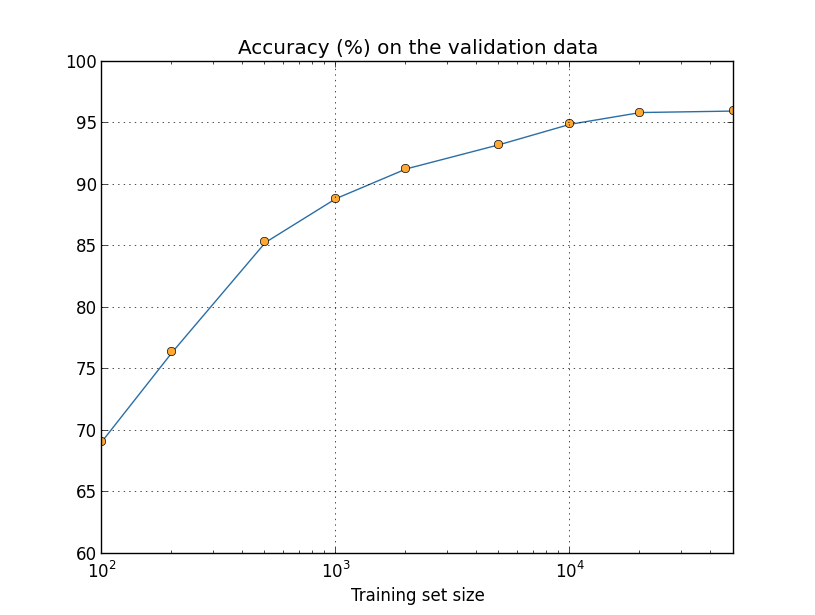
\includegraphics[width=0.867\textwidth]{images/more_data_log.png}
\end{center}

\noindent 假设我们不使用神经网络，而是使用其他一些机器学习技术来分类数字. 例如，让我们尝试使用我们在第 1 章简要介绍过的支持向量机（SVM）. 与第 1 章的情况一样，如果你不熟悉 SVM 也不用担心，我们不需要理解它们的细节. 相反，我们将使用 scikit-learn 库提供的 SVM. 下面是 SVM 性能随训练集大小变化的情况. 为了方便比较，我也绘制了神经网络的结果* \footnote{This graph was produced with the program more\_\allowbreak{}data.py (as were the last few graphs).}：

\begin{center}
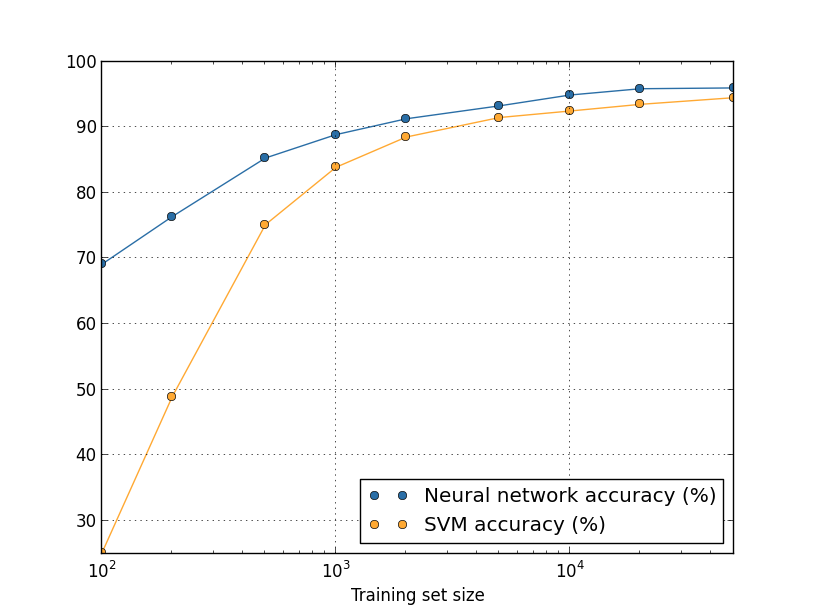
\includegraphics[width=0.867\textwidth]{images/more_data_comparison.png}
\end{center}

\noindent 关于这张图，可能首先让你注意到的是，对于每一种训练集大小，我们的神经网络都优于 SVM. 这很好，尽管你不应过度解读，因为我只是使用了 scikit-learn 的 SVM 的默认设置，而我们则做了相当多的工作来改进我们的神经网络. 关于这张图，一个更微妙但也更有趣的事实是，如果我们使用 50,000 张图像训练我们的 SVM，那么它的性能（94.48\% 准确率）实际上比我们的神经网络使用 5,000 张图像训练时的性能（93.24\% 准确率）更好. 换句话说，更多的训练数据有时可以弥补所使用的机器学习算法之间的差异.

甚至可能发生更有趣的事情. 假设我们试图使用两种机器学习算法，算法 A 和算法 B，来解决一个问题. 有时会发生算法 A 在一组训练数据上优于算法 B，而算法 B 在另一组不同的训练数据上优于算法 A 的情况. 我们在上面没有看到这种情况——那需要两条曲线交叉——但它确实会发生* \footnote{Striking examples may be found in Scaling to very very large corpora for natural language disambiguation, by Michele Banko and Eric Brill (2001).}. 对于问题``算法 A 比算法 B 更好吗？''，正确的回答实际上是：``你使用的是哪个训练数据集？''

所有这些都是需要牢记的警示，无论是在进行开发时，还是在阅读研究论文时. 许多论文专注于寻找新的技巧，以在标准基准数据集上榨取改进的性能.``我们的神奇技术使我们在标准基准 Y 上获得了 X\% 的提升''是研究声明的一种典型形式. 这类声明通常确实有趣，但必须理解为仅在所使用的特定训练数据集的背景下适用. 想象一个替代历史，在这个历史中，最初创建基准数据集的人获得了更多的研究经费. 他们可能会用这笔额外的钱来收集更多的训练数据. 那么，由神奇技术带来的``改进''完全有可能在更大的数据集上消失. 换句话说，所谓的改进可能只是历史的偶然. 要吸取的信息，尤其是在实际应用中，是我们既想要更好的算法\emph{也}想要更好的训练数据. 寻找更好的算法是好的，但要确保你没有只关注更好的算法，而忽略了获取更多或更好训练数据这些容易的胜利.

\end{exerciseBox}

\begin{exerciseBox}{习题}

\begin{itemize}

\item \textbf{（研究问题）} 我们的机器学习算法在非常大的数据集的极限情况下表现如何？对于任何给定的算法，很自然地会尝试在真正大数据的极限下定义渐近性能的概念. 解决这个问题的一个快速而粗略的方法是简单地尝试将曲线拟合到如上所示的图表，然后将拟合的曲线外推到无穷大. 这种方法的一个反对意见是，不同的曲线拟合方法会给出不同的渐近性能概念. 你能找到拟合到某个特定类别曲线的有原则的理由吗？如果能，请比较几种不同机器学习算法的渐近性能.

\end{itemize}

\textbf{总结：} 我们现在已经完成了对过拟合和正则化的深入探讨. 当然，我们还会再次回到这个问题. 正如我多次提到的，过拟合是神经网络中的一个主要问题，尤其是随着计算机变得更加强大，我们有能力训练更大的网络. 因此，迫切需要开发强大的正则化技术来减少过拟合，这是一个当前极其活跃的研究领域.

\end{exerciseBox}
\sectionTitle{权重初始化}{权重初始化}

当我们创建神经网络时，我们必须为初始权重和偏置做出选择. 到目前为止，我们一直按照我在第 1 章中简要讨论过的一个方案来选择它们. 提醒一下，那个方案是使用独立的高斯随机变量来选择权重和偏置，并归一化为均值为 $0$、标准差为 $1$. 虽然这种方法效果不错，但它相当 \emph{ad hoc}，值得重新审视，看看我们能否找到一种更好的方式来设置初始权重和偏置，或许还能帮助我们的神经网络学得更快.

事实证明，我们可以做得比用归一化高斯分布初始化好得多. 要理解原因，假设我们正在处理一个具有大量输入神经元的网络——比如 $1,000$ 个. 再假设我们使用了归一化高斯分布来初始化连接到第一个隐藏层的权重. 现在我将专门关注连接输入神经元到隐藏层中第一个神经元的权重，忽略网络的其余部分：

\begin{center}
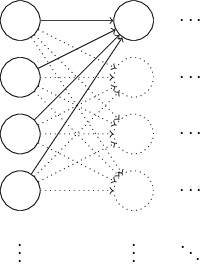
\includegraphics[width=0.9\textwidth]{images/tikz32.png}
\end{center}

\noindent 为简单起见，我们假设正在使用一个训练输入 $x$ 进行训练，其中一半的输入神经元是开启的，即设为 $1$，一半的输入神经元是关闭的，即设为 $0$. 接下来的论证更普遍地适用，但你会从这个特例中领会到要点. 让我们考虑隐藏神经元的输入的加权和 $z = \sum_j w_j x_j+b$. 这个和中有 $500$ 项消失了，因为对应的输入 $x_j$ 为零. 因此 $z$ 是总共 $501$ 个归一化高斯随机变量之和，包括 $500$ 个权重项和 $1$ 个额外的偏置项. 于是 $z$ 本身服从均值为零、标准差为 $\sqrt{501} \approx 22.4$ 的高斯分布. 也就是说，$z$ 具有非常宽的高斯分布，完全不是尖锐的峰值：特别地，我们可以从这个图中看到，$|z|$ 很可能会相当大，即要么 $z \gg 1$ 要么 $z \ll -1$. 如果是这种情况，那么隐藏神经元的输出 $\sigma(z)$ 将非常接近 $1$ 或 $0$. 这意味着我们的隐藏神经元将饱和. 当这种情况发生时，正如我们所知，对权重做微小改变只会对隐藏神经元的激活值产生极其微小的变化. 隐藏神经元激活值的这种微小变化反过来几乎完全不会影响网络中其余的神经元，我们也会看到代价函数相应地只有极其微小的变化. 结果，当我们使用梯度下降算法时，那些权重只会学习得非常慢*\footnote{我们在第 2 章中更详细地讨论了这一点，在那里我们使用反向传播方程来表明输入到饱和神经元的权重学习得很慢.}. 这类似于我们在本章前面讨论过的问题，即输出神经元在错误的值上饱和导致学习减慢. 我们通过巧妙选择代价函数解决了前面那个问题. 不幸的是，虽然那对饱和的输出神经元有帮助，但对饱和的隐藏神经元的问题完全无济于事.

我一直在谈论输入到第一个隐藏层的权重. 当然，类似的论证也适用于后面的隐藏层：如果后面隐藏层的权重使用归一化高斯分布初始化，那么激活值往往会非常接近 $0$ 或 $1$，学习将进行得非常缓慢.

有没有什么方法可以为权重和偏置选择更好的初始化，从而不会出现这种饱和，避免学习减慢？假设我们有一个具有 $n_{\rm in}$ 个输入权重的神经元. 那么我们将这些权重初始化为均值为 $0$、标准差为 $1/\sqrt{n_{\rm in}}$ 的高斯随机变量. 也就是说，我们将高斯分布压缩，使得我们的神经元不太可能饱和. 我们将继续把偏置选择为均值为 $0$、标准差为 $1$ 的高斯分布，原因我稍后会再谈. 有了这些选择，加权和 $z = \sum_j w_j x_j + b$ 将再次是一个均值为 $0$ 的高斯随机变量，但它会比之前尖锐得多. 假设像之前一样，$500$ 个输入为零，$500$ 个输入为 $1$. 那么很容易证明（见下面的练习）$z$ 服从均值为 $0$、标准差为 $\sqrt{3/2} = 1.22\ldots$ 的高斯分布. 这比之前尖锐得多，以至于下面的图甚至低估了这种情况，因为与之前的图相比，我不得不重新调整了纵轴的比例：这样的神经元饱和的可能性要小得多，相应地出现学习减慢问题的可能性也小得多.

\begin{exerciseBox}{练习}

\begin{itemize}

\item 验证上面段落中 $z = \sum_j w_j x_j + b$ 的标准差是 $\sqrt{3/2}$. 知道以下事实可能有帮助：(a) 独立随机变量之和的方差是各个随机变量方差之和；(b) 方差是标准差的平方.

\end{itemize}

我上面说过我们将像之前一样继续初始化偏置，即作为均值为 $0$、标准差为 $1$ 的高斯随机变量. 这是可以的，因为它不会使我们的神经元饱和的可能性增加太多. 事实上，我们如何初始化偏置并不太重要，只要避免饱和问题即可. 有些人甚至将所有偏置初始化为 $0$，依靠梯度下降来学习合适的偏置. 但由于这不太可能产生太大差异，我们将继续使用与之前相同的初始化过程.

让我们使用 MNIST 数字分类任务来比较新旧两种权重初始化方法的结果. 和之前一样，我们将使用 $30$ 个隐藏神经元、小批量大小为 $10$、正则化参数 $\lambda = 5.0$ 以及交叉熵代价函数. 我们将学习率从 $\eta = 0.5$ 略微降低到 $0.1$，因为这使结果在图中更容易看清. 我们可以使用旧的权重初始化方法进行训练：

\begin{lstlisting}
>>> import mnist_loader
>>> training_data, validation_data, test_data = \
... mnist_loader.load_data_wrapper()
>>> import network2
>>> net = network2.Network([784, 30, 10], cost=network2.CrossEntropyCost)
>>> net.large_weight_initializer()
>>> net.SGD(training_data, 30, 10, 0.1, lmbda = 5.0,
... evaluation_data=validation_data,
... monitor_evaluation_accuracy=True)

\end{lstlisting}

我们也可以使用新的权重初始化方法进行训练. 这实际上更容易，因为 network2 默认的权重初始化方式就是使用这种新方法. 这意味着我们可以省略上面的 net.large\_\allowbreak{}weight\_\allowbreak{}initializer() 调用：

\begin{lstlisting}
>>> net = network2.Network([784, 30, 10], cost=network2.CrossEntropyCost)
>>> net.SGD(training_data, 30, 10, 0.1, lmbda = 5.0,
... evaluation_data=validation_data,
... monitor_evaluation_accuracy=True)

\end{lstlisting}

绘制结果* *用于生成这张图和下一张图的程序是 weight\_\allowbreak{}initialization.py.

，我们得到：

\begin{center}
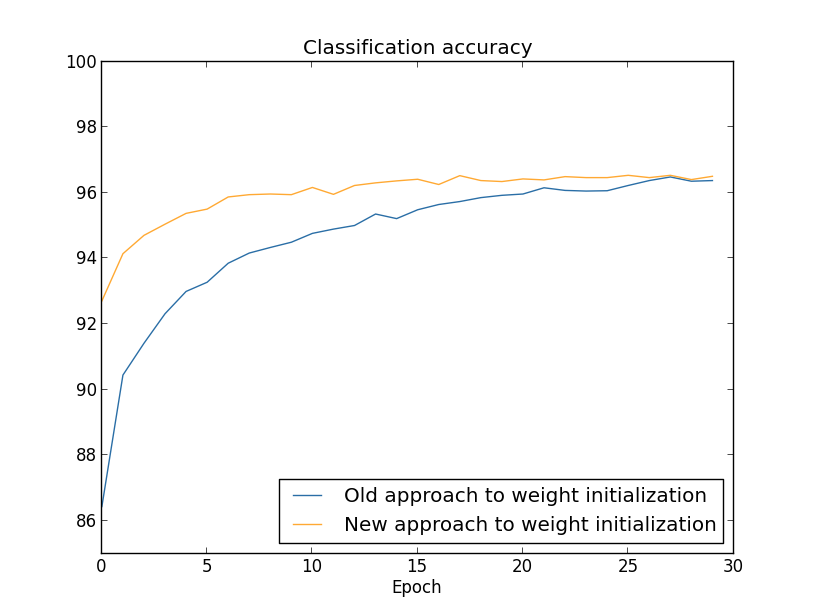
\includegraphics[width=0.867\textwidth]{images/weight_initialization_30.png}
\end{center}

\noindent 在两种情况下，我们最终得到的分类准确率都略高于 96\%. 最终的分类准确率在两种情况下几乎完全相同. 但新的初始化技术让我们更快、快得多地达到那里. 在第一个训练轮次结束时，旧的权重初始化方法的分类准确率不到 87\%，而新方法已经接近 93\%. 看起来正在发生的是，我们新的权重初始化方法让我们从一个好得多的状态开始，这使我们能够更快地获得好的结果. 如果我们用 $100$ 个隐藏神经元绘制结果，也会看到同样的现象：

\begin{center}
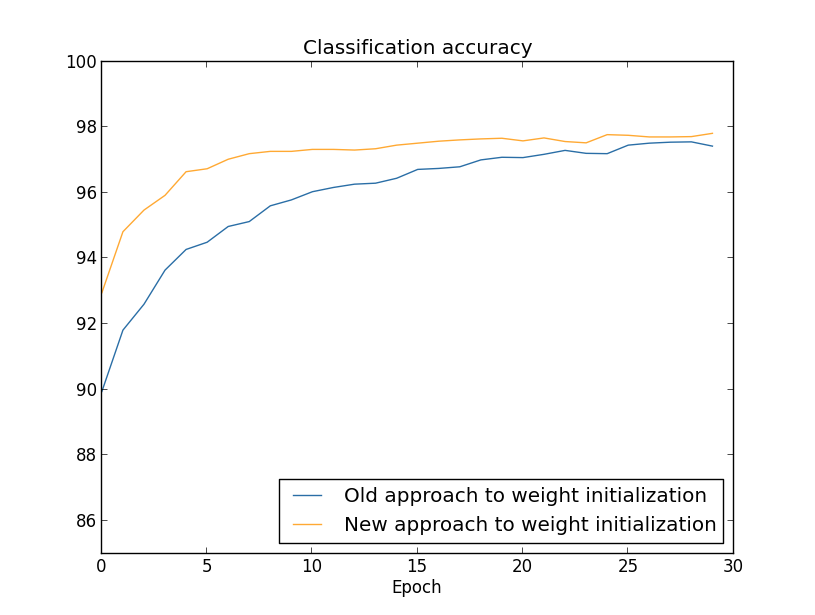
\includegraphics[width=0.867\textwidth]{images/weight_initialization_100.png}
\end{center}

\noindent 在这种情况下，两条曲线没有完全重合. 然而，我的实验表明，只需再训练几个轮次（未显示），准确率就会变得几乎完全相同. 因此，基于这些实验，看起来改进的权重初始化只是加速了学习，并没有改变我们网络的最终性能. 然而，在第 4 章中我们将看到一些神经网络的例子，其中长期行为在使用 $1/\sqrt{n_{\rm in}}$ 权重初始化时显著更好. 因此，不仅学习速度得到了改善，有时最终性能也得到了改善.

$1/\sqrt{n_{\rm in}}$ 权重初始化方法有助于改善我们神经网络的学习方式. 其他权重初始化技术也被提出过，许多都建立在这个基本思想之上. 我不会在这里回顾其他方法，因为 $1/\sqrt{n_{\rm in}}$ 对我们的目的来说已经足够好了. 如果你有兴趣进一步了解，我推荐看看 Yoshua Bengio 2012 年论文第 14 和 15 页的讨论*\footnote{Practical Recommendations for Gradient-Based Training of Deep Architectures, by Yoshua Bengio (2012).}，以及其中的参考文献.

\end{exerciseBox}

\begin{exerciseBox}{习题}

\begin{itemize}

\item \textbf{将正则化与改进的权重初始化方法联系起来} L2 正则化有时会自动给我们类似于新权重初始化方法的东西. 假设我们正在使用旧的权重初始化方法. 草拟一个启发式论证：(1) 假设 $\lambda$ 不太小，最初的几个训练轮次将几乎完全由权重衰减主导；(2) 只要 $\eta \lambda \ll n$，权重每轮次将按因子 $\exp(-\eta \lambda / m)$ 衰减；(3) 假设 $\lambda$ 不太大，当权重降到大约 $1/\sqrt{n}$ 的大小时，权重衰减将逐渐减弱，其中 $n$ 是网络中权重的总数. 论证这些条件在本节所绘制的例子中都得到了满足.

\end{itemize}

\end{exerciseBox}
\sectionTitle{重访手写数字识别：代码}{重访手写数字识别：代码}

让我们来实现本章中讨论过的想法. 我们将开发一个新程序 \texttt{network2.py}，它是我们在第 1 章中开发的程序 \texttt{network.py} 的改进版本. 如果你有一阵子没看过 \texttt{network.py} 了，那么花几分钟快速重读一下之前的讨论可能会对你有所帮助. 它只有 74 行代码，很容易理解.

和 \texttt{network.py} 中的情况一样，\texttt{network2.py} 的主角是 \texttt{Network} 类，我们用它来表示我们的神经网络. 我们用一个包含网络中各个层 \texttt{sizes} 的列表，以及一个要使用的 \texttt{cost} 选择来初始化 \texttt{Network} 的一个实例，默认使用交叉熵：

\begin{lstlisting}
class Network(object):

    def __init__(self, sizes, cost=CrossEntropyCost):
        self.num_layers = len(sizes)
        self.sizes = sizes
        self.default_weight_initializer()
        self.cost=cost

\end{lstlisting}

\texttt{\_\allowbreak{}\_\allowbreak{}init\_\allowbreak{}\_\allowbreak{}} 方法的前几行与 \texttt{network.py} 中相同，而且相当不言自明. 但接下来的两行是新的，我们需要详细理解它们在做什么.

让我们从考察 \texttt{default\_\allowbreak{}weight\_\allowbreak{}initializer} 方法开始. 它利用了我们新的、改进过的权重初始化方法. 正如我们所见，在该方法中，输入到一个神经元的权重被初始化为均值为 0、标准差为 $1$ 除以输入到该神经元的连接数的平方根的高斯随机变量. 同样在这个方法中，我们将初始化偏置，使用均值为 $0$、标准差为 $1$ 的高斯随机变量. 代码如下：

\begin{lstlisting}
    def default_weight_initializer(self):
        self.biases = [np.random.randn(y, 1) for y in self.sizes[1:]]
        self.weights = [np.random.randn(y, x)/np.sqrt(x)
                        for x, y in zip(self.sizes[:-1], self.sizes[1:])]

\end{lstlisting}

要理解这段代码，回忆一下 \texttt{np} 是用于进行线性代数的 Numpy 库可能会有所帮助. 我们会在程序开头 \texttt{import} Numpy. 另外，注意我们没有为第一层神经元初始化任何偏置. 我们避免这样做是因为第一层是输入层，因此任何偏置都不会被用到. 我们在 \texttt{network.py} 中做的完全一样.

作为 \texttt{default\_\allowbreak{}weight\_\allowbreak{}initializer} 的补充，我们还会包含一个 \texttt{large\_\allowbreak{}weight\_\allowbreak{}initializer} 方法. 这个方法使用第 1 章中的旧方法初始化权重和偏置，将权重和偏置都初始化为均值为 $0$、标准差为 $1$ 的高斯随机变量. 当然，这段代码与 \texttt{default\_\allowbreak{}weight\_\allowbreak{}initializer} 只有一点点不同：

\begin{lstlisting}
    def large_weight_initializer(self):
        self.biases = [np.random.randn(y, 1) for y in self.sizes[1:]]
        self.weights = [np.random.randn(y, x)
                        for x, y in zip(self.sizes[:-1], self.sizes[1:])]

\end{lstlisting}

我包含 \texttt{large\_\allowbreak{}weight\_\allowbreak{}initializer} 方法主要是为了方便，使本章的结果更容易与第 1 章的结果进行比较. 我想不出有多少实际情形会让我推荐使用它！

\texttt{Network} 的 \texttt{\_\allowbreak{}\_\allowbreak{}init\_\allowbreak{}\_\allowbreak{}} 方法中的第二个新事物是我们现在初始化了一个 \texttt{cost} 属性. 要理解它是如何工作的，让我们看看我们用来表示交叉熵代价的类*\footnote{如果你不熟悉 Python 的静态方法，你可以忽略 \texttt{@staticmethod} 装饰器，只把 \texttt{fn} 和 \texttt{delta} 当作普通方法即可. 如果你对细节感到好奇，\texttt{@staticmethod} 所做的只是告诉 Python 解释器，紧随其后的方法不以任何方式依赖于对象. 这就是为什么 \texttt{self} 没有作为参数传递给 \texttt{fn} 和 \texttt{delta} 方法.}：

\begin{lstlisting}
class CrossEntropyCost(object):

    @staticmethod
    def fn(a, y):
        return np.sum(np.nan_to_num(-y*np.log(a)-(1-y)*np.log(1-a)))

    @staticmethod
    def delta(z, a, y):
        return (a-y)

\end{lstlisting}

让我们来分解一下. 首先要观察到的是，尽管从数学上说交叉熵是一个函数，但我们把它实现为一个 Python 类，而不是一个 Python 函数. 我为什么做出这个选择？原因是代价在我们的网络中扮演两种不同的角色. 显而易见的角色是，它是输出激活值 \texttt{a} 与期望输出 \texttt{y} 匹配程度的度量. 这个角色由 \texttt{CrossEntropyCost.fn} 方法承担. （顺便注意，\texttt{CrossEntropyCost.fn} 内部的 \texttt{np.nan\_\allowbreak{}to\_\allowbreak{}num} 调用确保 Numpy 正确处理非常接近于零的数的对数.）但代价函数进入我们网络还有第二种方式. 回忆第 2 章，在运行反向传播算法时，我们需要计算网络的输出误差 $\delta^L$. 输出误差的形式取决于代价函数的选择：不同的代价函数，输出误差的形式不同. 对于交叉熵，输出误差正如我们在公式 (66) 中所见

\begin{align*}
\delta^L = a^L-y. \nonumber
\end{align*}

\noindent，

\begin{equation}
\delta^L = a^L-y.
\tag{99}
\end{equation}

\noindent 出于这个原因，我们定义了第二个方法 \texttt{CrossEntropyCost.delta}，其目的是告诉我们的网络如何计算输出误差. 然后我们把这两个方法打包进一个单独的类中，其中包含我们的网络需要知道的关于代价函数的一切.

以类似的方式，\texttt{network2.py} 还包含一个表示二次代价函数的类. 包含它是为了与第 1 章的结果进行比较，因为往后我们将主要使用交叉熵. 代码就在下面. \texttt{QuadraticCost.fn} 方法是对与实际输出 \texttt{a} 和期望输出 \texttt{y} 相关联的二次代价的直接计算. \texttt{QuadraticCost.delta} 返回的值基于表达式 (30)

\begin{align*}
\delta^L = (a^L-y) \odot \sigma'(z^L) \nonumber
\end{align*}

\noindent 即二次代价的输出误差，这是我们在第 2 章中推导出来的.

\begin{lstlisting}
class QuadraticCost(object):

    @staticmethod
    def fn(a, y):
        return 0.5*np.linalg.norm(a-y)**2

    @staticmethod
    def delta(z, a, y):
        return (a-y) * sigmoid_prime(z)

\end{lstlisting}

我们现在已经理解了 \texttt{network2.py} 与 \texttt{network.py} 之间的主要区别. 全都是相当简单的东西. 还有一些较小的改动，我将在下面讨论，包括 L2 正则化的实现. 在讨论这些之前，让我们看看 \texttt{network2.py} 的完整代码. 你不需要详细阅读所有代码，但值得理解其大致结构，尤其是阅读文档字符串，这样你就能理解程序的每一部分在做什么. 当然，也欢迎你按自己的意愿深入钻研！如果你迷失了方向，不妨继续阅读下面的正文，稍后再回到代码. 总之，代码如下：

\begin{lstlisting}
"""network2.py
~~~~~~~~~~~~~~

An improved version of network.py, implementing the stochastic
gradient descent learning algorithm for a feedforward neural network.
Improvements include the addition of the cross-entropy cost function,
regularization, and better initialization of network weights.  Note
that I have focused on making the code simple, easily readable, and
easily modifiable.  It is not optimized, and omits many desirable
features.

"""

#### Libraries
# Standard library
import json
import random
import sys

# Third-party libraries
import numpy as np

#### Define the quadratic and cross-entropy cost functions

class QuadraticCost(object):

    @staticmethod
    def fn(a, y):
        """Return the cost associated with an output ``a`` and desired output
        ``y``.

        """
        return 0.5*np.linalg.norm(a-y)**2

    @staticmethod
    def delta(z, a, y):
        """Return the error delta from the output layer."""
        return (a-y) * sigmoid_prime(z)

class CrossEntropyCost(object):

    @staticmethod
    def fn(a, y):
        """Return the cost associated with an output ``a`` and desired output
        ``y``.  Note that np.nan_to_num is used to ensure numerical
        stability.  In particular, if both ``a`` and ``y`` have a 1.0
        in the same slot, then the expression (1-y)*np.log(1-a)
        returns nan.  The np.nan_to_num ensures that that is converted
        to the correct value (0.0).

        """
        return np.sum(np.nan_to_num(-y*np.log(a)-(1-y)*np.log(1-a)))

    @staticmethod
    def delta(z, a, y):
        """Return the error delta from the output layer.  Note that the
        parameter ``z`` is not used by the method.  It is included in
        the method's parameters in order to make the interface
        consistent with the delta method for other cost classes.

        """
        return (a-y)

#### Main Network class
class Network(object):

    def __init__(self, sizes, cost=CrossEntropyCost):
        """The list ``sizes`` contains the number of neurons in the respective
        layers of the network.  For example, if the list was [2, 3, 1]
        then it would be a three-layer network, with the first layer
        containing 2 neurons, the second layer 3 neurons, and the
        third layer 1 neuron.  The biases and weights for the network
        are initialized randomly, using
        ``self.default_weight_initializer`` (see docstring for that
        method).

        """
        self.num_layers = len(sizes)
        self.sizes = sizes
        self.default_weight_initializer()
        self.cost=cost

    def default_weight_initializer(self):
        """Initialize each weight using a Gaussian distribution with mean 0
        and standard deviation 1 over the square root of the number of
        weights connecting to the same neuron.  Initialize the biases
        using a Gaussian distribution with mean 0 and standard
        deviation 1.

        Note that the first layer is assumed to be an input layer, and
        by convention we won't set any biases for those neurons, since
        biases are only ever used in computing the outputs from later
        layers.

        """
        self.biases = [np.random.randn(y, 1) for y in self.sizes[1:]]
        self.weights = [np.random.randn(y, x)/np.sqrt(x)
                        for x, y in zip(self.sizes[:-1], self.sizes[1:])]

    def large_weight_initializer(self):
        """Initialize the weights using a Gaussian distribution with mean 0
        and standard deviation 1.  Initialize the biases using a
        Gaussian distribution with mean 0 and standard deviation 1.

        Note that the first layer is assumed to be an input layer, and
        by convention we won't set any biases for those neurons, since
        biases are only ever used in computing the outputs from later
        layers.

        This weight and bias initializer uses the same approach as in
        Chapter 1, and is included for purposes of comparison.  It
        will usually be better to use the default weight initializer
        instead.

        """
        self.biases = [np.random.randn(y, 1) for y in self.sizes[1:]]
        self.weights = [np.random.randn(y, x)
                        for x, y in zip(self.sizes[:-1], self.sizes[1:])]

    def feedforward(self, a):
        """Return the output of the network if ``a`` is input."""
        for b, w in zip(self.biases, self.weights):
            a = sigmoid(np.dot(w, a)+b)
        return a

    def SGD(self, training_data, epochs, mini_batch_size, eta,
            lmbda = 0.0,
            evaluation_data=None,
            monitor_evaluation_cost=False,
            monitor_evaluation_accuracy=False,
            monitor_training_cost=False,
            monitor_training_accuracy=False):
        """Train the neural network using mini-batch stochastic gradient
        descent.  The ``training_data`` is a list of tuples ``(x, y)``
        representing the training inputs and the desired outputs.  The
        other non-optional parameters are self-explanatory, as is the
        regularization parameter ``lmbda``.  The method also accepts
        ``evaluation_data``, usually either the validation or test
        data.  We can monitor the cost and accuracy on either the
        evaluation data or the training data, by setting the
        appropriate flags.  The method returns a tuple containing four
        lists: the (per-epoch) costs on the evaluation data, the
        accuracies on the evaluation data, the costs on the training
        data, and the accuracies on the training data.  All values are
        evaluated at the end of each training epoch.  So, for example,
        if we train for 30 epochs, then the first element of the tuple
        will be a 30-element list containing the cost on the
        evaluation data at the end of each epoch. Note that the lists
        are empty if the corresponding flag is not set.

        """
        if evaluation_data: n_data = len(evaluation_data)
        n = len(training_data)
        evaluation_cost, evaluation_accuracy = [], []
        training_cost, training_accuracy = [], []
        for j in xrange(epochs):
            random.shuffle(training_data)
            mini_batches = [
                training_data[k:k+mini_batch_size]
                for k in xrange(0, n, mini_batch_size)]
            for mini_batch in mini_batches:
                self.update_mini_batch(
                    mini_batch, eta, lmbda, len(training_data))
            print "Epoch
            if monitor_training_cost:
                cost = self.total_cost(training_data, lmbda)
                training_cost.append(cost)
                print "Cost on training data: {}".format(cost)
            if monitor_training_accuracy:
                accuracy = self.accuracy(training_data, convert=True)
                training_accuracy.append(accuracy)
                print "Accuracy on training data: {} / {}".format(
                    accuracy, n)
            if monitor_evaluation_cost:
                cost = self.total_cost(evaluation_data, lmbda, convert=True)
                evaluation_cost.append(cost)
                print "Cost on evaluation data: {}".format(cost)
            if monitor_evaluation_accuracy:
                accuracy = self.accuracy(evaluation_data)
                evaluation_accuracy.append(accuracy)
                print "Accuracy on evaluation data: {} / {}".format(
                    self.accuracy(evaluation_data), n_data)
            print
        return evaluation_cost, evaluation_accuracy, \
            training_cost, training_accuracy

    def update_mini_batch(self, mini_batch, eta, lmbda, n):
        """Update the network's weights and biases by applying gradient
        descent using backpropagation to a single mini batch.  The
        ``mini_batch`` is a list of tuples ``(x, y)``, ``eta`` is the
        learning rate, ``lmbda`` is the regularization parameter, and
        ``n`` is the total size of the training data set.

        """
        nabla_b = [np.zeros(b.shape) for b in self.biases]
        nabla_w = [np.zeros(w.shape) for w in self.weights]
        for x, y in mini_batch:
            delta_nabla_b, delta_nabla_w = self.backprop(x, y)
            nabla_b = [nb+dnb for nb, dnb in zip(nabla_b, delta_nabla_b)]
            nabla_w = [nw+dnw for nw, dnw in zip(nabla_w, delta_nabla_w)]
        self.weights = [(1-eta*(lmbda/n))*w-(eta/len(mini_batch))*nw
                        for w, nw in zip(self.weights, nabla_w)]
        self.biases = [b-(eta/len(mini_batch))*nb
                       for b, nb in zip(self.biases, nabla_b)]

    def backprop(self, x, y):
        """Return a tuple ``(nabla_b, nabla_w)`` representing the
        gradient for the cost function C_x.  ``nabla_b`` and
        ``nabla_w`` are layer-by-layer lists of numpy arrays, similar
        to ``self.biases`` and ``self.weights``."""
        nabla_b = [np.zeros(b.shape) for b in self.biases]
        nabla_w = [np.zeros(w.shape) for w in self.weights]
        # feedforward
        activation = x
        activations = [x] # list to store all the activations, layer by layer
        zs = [] # list to store all the z vectors, layer by layer
        for b, w in zip(self.biases, self.weights):
            z = np.dot(w, activation)+b
            zs.append(z)
            activation = sigmoid(z)
            activations.append(activation)
        # backward pass
        delta = (self.cost).delta(zs[-1], activations[-1], y)
        nabla_b[-1] = delta
        nabla_w[-1] = np.dot(delta, activations[-2].transpose())
        # Note that the variable l in the loop below is used a little
        # differently to the notation in Chapter 2 of the book.  Here,
        # l = 1 means the last layer of neurons, l = 2 is the
        # second-last layer, and so on.  It's a renumbering of the
        # scheme in the book, used here to take advantage of the fact
        # that Python can use negative indices in lists.
        for l in xrange(2, self.num_layers):
            z = zs[-l]
            sp = sigmoid_prime(z)
            delta = np.dot(self.weights[-l+1].transpose(), delta) * sp
            nabla_b[-l] = delta
            nabla_w[-l] = np.dot(delta, activations[-l-1].transpose())
        return (nabla_b, nabla_w)

    def accuracy(self, data, convert=False):
        """Return the number of inputs in ``data`` for which the neural
        network outputs the correct result. The neural network's
        output is assumed to be the index of whichever neuron in the
        final layer has the highest activation.

        The flag ``convert`` should be set to False if the data set is
        validation or test data (the usual case), and to True if the
        data set is the training data. The need for this flag arises
        due to differences in the way the results ``y`` are
        represented in the different data sets.  In particular, it
        flags whether we need to convert between the different
        representations.  It may seem strange to use different
        representations for the different data sets.  Why not use the
        same representation for all three data sets?  It's done for
        efficiency reasons -- the program usually evaluates the cost
        on the training data and the accuracy on other data sets.
        These are different types of computations, and using different
        representations speeds things up.  More details on the
        representations can be found in
        mnist_loader.load_data_wrapper.

        """
        if convert:
            results = [(np.argmax(self.feedforward(x)), np.argmax(y))
                       for (x, y) in data]
        else:
            results = [(np.argmax(self.feedforward(x)), y)
                        for (x, y) in data]
        return sum(int(x == y) for (x, y) in results)

    def total_cost(self, data, lmbda, convert=False):
        """Return the total cost for the data set ``data``.  The flag
        ``convert`` should be set to False if the data set is the
        training data (the usual case), and to True if the data set is
        the validation or test data.  See comments on the similar (but
        reversed) convention for the ``accuracy`` method, above.
        """
        cost = 0.0
        for x, y in data:
            a = self.feedforward(x)
            if convert: y = vectorized_result(y)
            cost += self.cost.fn(a, y)/len(data)
        cost += 0.5*(lmbda/len(data))*sum(
            np.linalg.norm(w)**2 for w in self.weights)
        return cost

    def save(self, filename):
        """Save the neural network to the file ``filename``."""
        data = {"sizes": self.sizes,
                "weights": [w.tolist() for w in self.weights],
                "biases": [b.tolist() for b in self.biases],
                "cost": str(self.cost.__name__)}
        f = open(filename, "w")
        json.dump(data, f)
        f.close()

#### Loading a Network
def load(filename):
    """Load a neural network from the file ``filename``.  Returns an
    instance of Network.

    """
    f = open(filename, "r")
    data = json.load(f)
    f.close()
    cost = getattr(sys.modules[__name__], data["cost"])
    net = Network(data["sizes"], cost=cost)
    net.weights = [np.array(w) for w in data["weights"]]
    net.biases = [np.array(b) for b in data["biases"]]
    return net

#### Miscellaneous functions
def vectorized_result(j):
    """Return a 10-dimensional unit vector with a 1.0 in the j'th position
    and zeroes elsewhere.  This is used to convert a digit (0...9)
    into a corresponding desired output from the neural network.

    """
    e = np.zeros((10, 1))
    e[j] = 1.0
    return e

def sigmoid(z):
    """The sigmoid function."""
    return 1.0/(1.0+np.exp(-z))

def sigmoid_prime(z):
    """Derivative of the sigmoid function."""
    return sigmoid(z)*(1-sigmoid(z))

\end{lstlisting}
代码中比较有趣的一个变化是加入了 L2 正则化. 虽然这是一个概念上的重大改变，但实现起来却微不足道，以至于在代码中很容易被忽略. 大部分情况下，它只是把参数 \texttt{lmbda} 传给各种方法，尤其是 \texttt{Network.SGD} 方法. 真正的工作由程序中的一行完成，即 \texttt{Network.update\_\allowbreak{}mini\_\allowbreak{}batch} 方法的倒数第四行. 正是在那里，我们修改了梯度下降的更新规则以包含权重衰减. 但尽管这个修改很小，它对结果却有巨大的影响！

顺便说一句，在神经网络中实现新技术时，这是很常见的. 我们花了数千字讨论正则化. 它在概念上相当微妙且难以理解. 然而把它加入我们的程序却是微不足道的！复杂的技术可以通过对代码的小改动来实现，这种情况出奇地常见.

我们代码中另一个小而重要的改动是给随机梯度下降方法 \texttt{Network.SGD} 增加了几个可选标志. 这些标志使得我们可以监控 \texttt{training\_\allowbreak{}data} 上的代价和准确率，或者监控可以传给 \texttt{Network.SGD} 的一组 \texttt{evaluation\_\allowbreak{}data} 上的代价和准确率. 我们在本章前面已经多次使用过这些标志，但让我举一个例子说明它是如何工作的，只是为了提醒你一下：

\begin{lstlisting}
>>> import mnist_loader
>>> training_data, validation_data, test_data = \
... mnist_loader.load_data_wrapper()
>>> import network2
>>> net = network2.Network([784, 30, 10], cost=network2.CrossEntropyCost)
>>> net.SGD(training_data, 30, 10, 0.5,
... lmbda = 5.0,
... evaluation_data=validation_data,
... monitor_evaluation_accuracy=True,
... monitor_evaluation_cost=True,
... monitor_training_accuracy=True,
... monitor_training_cost=True)

\end{lstlisting}

这里，我们把 \texttt{evaluation\_\allowbreak{}data} 设为 \texttt{validation\_\allowbreak{}data}. 但我们也可以监控 \texttt{test\_\allowbreak{}data} 或任何其他数据集上的性能. 我们还有四个标志，告诉我们要监控 \texttt{evaluation\_\allowbreak{}data} 和 \texttt{training\_\allowbreak{}data} 上的代价和准确率. 这些标志默认是 \texttt{False}，但这里被打开了，以便监控我们的 \texttt{Network} 的性能. 此外， \texttt{network2.py} 的 \texttt{Network.SGD} 方法返回一个四元组，表示监控的结果. 我们可以这样使用它：

\begin{lstlisting}
>>> evaluation_cost, evaluation_accuracy,
... training_cost, training_accuracy = net.SGD(training_data, 30, 10, 0.5,
... lmbda = 5.0,
... evaluation_data=validation_data,
... monitor_evaluation_accuracy=True,
... monitor_evaluation_cost=True,
... monitor_training_accuracy=True,
... monitor_training_cost=True)

\end{lstlisting}

所以，例如， \texttt{evaluation\_\allowbreak{}cost} 将是一个包含 30 个元素的列表，其中保存了每个轮次结束时评估数据上的代价. 这类信息对于理解网络的行为极其有用. 例如，它可以用来绘制图表，显示网络如何随时间学习. 事实上，这正是我在本章前面构建所有图表的方式. 但请注意，如果任何监控标志没有被设置，那么元组中对应的元素将是空列表.

代码中的其他新增内容包括一个 \texttt{Network.save} 方法，用于把 \texttt{Network} 对象保存到磁盘，以及一个稍后把它们 \texttt{load} 回来的函数. 请注意，保存和加载是使用 JSON 完成的，而不是 Python 的 \texttt{pickle} 或 \texttt{cPickle} 模块，后者是我们在 Python 中把对象保存到磁盘和从磁盘加载对象的常用方式. 使用 JSON 比使用 \texttt{pickle} 或 \texttt{cPickle} 需要更多的代码. 要理解我为什么使用 JSON，想象一下未来某个时候我们决定修改 \texttt{Network} 类，以允许使用 S 型神经元以外的神经元. 要实现这个改变，我们很可能会修改 \texttt{Network.\_\allowbreak{}\_\allowbreak{}init\_\allowbreak{}\_\allowbreak{}} 方法中定义的属性. 如果我们只是简单地 pickle 了对象，那会导致我们的 \texttt{load} 函数失败. 使用 JSON 显式地进行序列化，可以很容易地确保旧的 \texttt{Network} 仍然能够 \texttt{load}.

\texttt{network2.py} 的代码中还有许多其他小改动，但它们都只是 \texttt{network.py} 的简单变体. 最终结果是，我们那个 74 行的程序扩展成了一个功能强大得多的 152 行程序.

\begin{exerciseBox}{习题}

\begin{itemize}

\item 修改上面的代码以实现 L1 正则化，并使用 L1 正则化通过一个含 $30$ 个隐藏神经元的网络来分类 MNIST 数字. 你能找到一个正则化参数，使你做得比运行未正则化的网络更好吗？

\item 看一看 \texttt{network.py} 中的 \texttt{Network.cost\_\allowbreak{}derivative} 方法. 那个方法是为二次代价编写的. 你会如何为交叉熵代价重写这个方法？你能想到交叉熵版本中可能出现的一个问题吗？在 \texttt{network2.py} 中，我们完全消除了 \texttt{Network.cost\_\allowbreak{}derivative} 方法，而是把它的功能并入 \texttt{CrossEntropyCost.delta} 方法. 这如何解决你刚刚发现的问题？

\end{itemize}

\end{exerciseBox}
\sectionTitle{如何选择神经网络的超参数？}{如何选择神经网络的超参数？}

到目前为止，我还没有解释过我是如何为学习率 $\eta$、正则化参数 $\lambda$ 等超参数选择取值的. 我只是给出了一些效果还不错的取值. 在实践中，当你使用神经网络来解决一个问题时，找到好的超参数可能很困难. 例如，想象一下我们刚刚接触到 MNIST 问题，并开始着手解决它，对应该使用什么超参数一无所知. 假设我们运气不错，在最初的实验中，我们按照本章前面所做的相同方式选择了许多超参数：30 个隐藏神经元、小批量大小为 10、使用交叉熵训练 30 个轮次. 但我们选择了学习率 $\eta = 10.0$ 和正则化参数 $\lambda = 1000.0$. 以下是我在某次这样的运行中看到的结果：

\begin{lstlisting}
>>> import mnist_loader
>>> training_data, validation_data, test_data = \
... mnist_loader.load_data_wrapper()
>>> import network2
>>> net = network2.Network([784, 30, 10])
>>> net.SGD(training_data, 30, 10, 10.0, lmbda = 1000.0,
... evaluation_data=validation_data, monitor_evaluation_accuracy=True)
Epoch 0 training complete
Accuracy on evaluation data: 1030 / 10000

Epoch 1 training complete
Accuracy on evaluation data: 990 / 10000

Epoch 2 training complete
Accuracy on evaluation data: 1009 / 10000

...

Epoch 27 training complete
Accuracy on evaluation data: 1009 / 10000

Epoch 28 training complete
Accuracy on evaluation data: 983 / 10000

Epoch 29 training complete
Accuracy on evaluation data: 967 / 10000

\end{lstlisting}

我们的分类准确率并不比随机猜测更好！我们的网络表现得就像一个随机噪声生成器！

``嗯，这很容易解决''，你可能会说，``只要降低学习率和正则化超参数就行了''. 不幸的是，你\emph{先验地}并不知道这些就是你需要调整的超参数. 也许真正的问题在于我们的 30 个隐藏神经元网络永远无法很好地工作，无论其他超参数如何选择？也许我们真的需要至少 100 个隐藏神经元？或者 300 个隐藏神经元？或者多个隐藏层？或者用不同的方式来编码输出？也许我们的网络正在学习，但我们需要训练更多的轮次？也许小批量太小了？也许换回二次代价函数会更好？也许我们需要尝试一种不同的权重初始化方法？如此等等，无穷无尽. 在超参数空间中很容易感到迷失. 如果你的网络非常大，或者使用了大量训练数据，这可能会特别令人沮丧，因为你可能训练了数小时、数天甚至数周，却毫无结果. 如果这种情况持续下去，它会打击你的信心. 也许神经网络是解决你问题的错误方法？也许你应该辞掉工作去养蜂？

在本节中，我将解释一些可用于设置神经网络超参数的启发式方法. 目标是帮助你建立一套工作流程，使你能够相当出色地设置超参数. 当然，我不会涵盖超参数优化的所有内容. 那是一个巨大的课题，而且无论如何，它都不是一个能被完全解决的问题，实践者们对于应该使用什么正确策略也没有普遍共识. 总还有更多的技巧可以尝试，从你的网络中榨取一点额外的性能. 但本节中的启发式方法应该能让你入门.\textbf{总体策略：}当使用神经网络来解决一个新问题时，第一个挑战是获得\emph{任何}非平凡的学习效果，即让网络取得比随机猜测更好的结果. 这可能出奇地困难，尤其是在面对一类新问题时. 让我们来看看如果你遇到这种麻烦时可以使用的策略.

例如，假设你是第一次攻克 MNIST. 你开始时热情高涨，但当你的第一个网络完全失败时（如上面的例子所示），你会有点气馁. 正确的做法是把问题简化. 去掉所有训练和验证图像，只保留数字为 0 或 1 的图像. 然后尝试训练一个网络来区分 0 和 1. 这不仅是一个本质上比区分全部十个数字更容易的问题，而且它还将训练数据量减少了 80\%，使训练速度提高了 5 倍. 这使你能够更快速地进行实验，从而更快地洞察如何构建一个好的网络.

你可以通过将网络精简为最有可能进行有意义学习的最简单网络，来进一步加速实验. 如果你相信一个 \texttt{[784, 10]} 网络很可能能够对 MNIST 数字进行比随机猜测更好的分类，那么就用这样的网络开始你的实验. 它将比训练一个 \texttt{[784, 30, 10]} 网络快得多，之后你可以逐步构建回后者.

你还可以通过提高监控频率来进一步加速实验. 在 \texttt{network2.py} 中，我们在每个训练轮次结束时监控性能. 每个轮次有 50,000 张图像，这意味着在获得关于网络学习效果的反馈之前需要等待一会儿——在我的笔记本电脑上训练一个 \texttt{[784, 30, 10]} 网络时，每个轮次大约需要十秒钟. 当然，十秒钟并不算长，但如果你想尝试几十种超参数选择，这就很烦人；如果你想尝试数百或数千种选择，那就开始让人难以忍受了. 我们可以通过更频繁地监控验证准确率来更快地获得反馈，比如每 1,000 张训练图像之后. 此外，我们可以不用完整的 10,000 张验证集来监控性能，而是仅用 100 张验证图像来获得一个快得多的估计. 重要的是网络看到足够多的图像来进行真正的学习，并获得一个相当好的粗略性能估计. 当然，我们的程序 \texttt{network2.py} 目前并不进行这种监控. 但为了在说明目的上达到类似效果的权宜之计，我们将把训练数据精简为仅前 1,000 张 MNIST 训练图像. 让我们试试看会发生什么.（为了保持下面的代码简单，我没有实现仅使用 0 和 1 图像的想法. 当然，只需稍多做一些工作就可以实现.）

\begin{lstlisting}
>>> net = network2.Network([784, 10])
>>> net.SGD(training_data[:1000], 30, 10, 10.0, lmbda = 1000.0, \
... evaluation_data=validation_data[:100], \
... monitor_evaluation_accuracy=True)
Epoch 0 training complete
Accuracy on evaluation data: 10 / 100

Epoch 1 training complete
Accuracy on evaluation data: 10 / 100

Epoch 2 training complete
Accuracy on evaluation data: 10 / 100
...

\end{lstlisting}

我们仍然得到纯粹的噪声！但有一个巨大的好处：我们现在可以在不到一秒的时间内获得反馈，而不是每十秒左右才获得一次. 这意味着你可以更快地尝试其他超参数选择，甚至可以几乎同时进行试验许多不同超参数选择的实验.

在上面的例子中，我保持 $\lambda$ 为 $\lambda = 1000.0$，正如我们之前所用的. 但由于我们改变了训练样本的数量，我们实际上应该改变 $\lambda$ 以保持权重衰减不变. 这意味着将 $\lambda$ 改为 $20.0$. 如果我们这样做，那么会发生以下情况：

\begin{lstlisting}
>>> net = network2.Network([784, 10])
>>> net.SGD(training_data[:1000], 30, 10, 10.0, lmbda = 20.0, \
... evaluation_data=validation_data[:100], \
... monitor_evaluation_accuracy=True)
Epoch 0 training complete
Accuracy on evaluation data: 12 / 100

Epoch 1 training complete
Accuracy on evaluation data: 14 / 100

Epoch 2 training complete
Accuracy on evaluation data: 25 / 100

Epoch 3 training complete
Accuracy on evaluation data: 18 / 100
...

\end{lstlisting}

啊哈！我们有了一个信号. 不是一个非常好的信号，但仍然是一个信号. 这是我们可以在此基础上继续发展的东西，通过修改超参数来尝试获得进一步的改进. 也许我们猜测我们的学习率需要更高.（你或许意识到，这是一个愚蠢的猜测，原因我们稍后会讨论，但请耐心听我说.）所以为了测试我们的猜测，我们尝试将 $\eta$ 调到 $100.0$：

\begin{lstlisting}
>>> net = network2.Network([784, 10])
>>> net.SGD(training_data[:1000], 30, 10, 100.0, lmbda = 20.0, \
... evaluation_data=validation_data[:100], \
... monitor_evaluation_accuracy=True)
Epoch 0 training complete
Accuracy on evaluation data: 10 / 100

Epoch 1 training complete
Accuracy on evaluation data: 10 / 100

Epoch 2 training complete
Accuracy on evaluation data: 10 / 100

Epoch 3 training complete
Accuracy on evaluation data: 10 / 100

...

\end{lstlisting}

这不行！这表明我们的猜测是错误的，问题并不是学习率太低. 所以相反，我们尝试将 $\eta$ 调到 $\eta = 1.0$：

\begin{lstlisting}
>>> net = network2.Network([784, 10])
>>> net.SGD(training_data[:1000], 30, 10, 1.0, lmbda = 20.0, \
... evaluation_data=validation_data[:100], \
... monitor_evaluation_accuracy=True)
Epoch 0 training complete
Accuracy on evaluation data: 62 / 100

Epoch 1 training complete
Accuracy on evaluation data: 42 / 100

Epoch 2 training complete
Accuracy on evaluation data: 43 / 100

Epoch 3 training complete
Accuracy on evaluation data: 61 / 100

...

\end{lstlisting}

这好多了！于是我们可以继续，逐个调整每个超参数，逐步提高性能. 一旦我们探索找到了 $\eta$ 的改进值，然后我们继续寻找 $\lambda$ 的好值. 然后尝试一个更复杂的架构，比如一个有 10 个隐藏神经元的网络. 然后再次调整 $\eta$ 和 $\lambda$ 的值. 然后增加到 20 个隐藏神经元. 然后再调整其他超参数. 如此继续，在每个阶段使用我们留出的验证数据来评估性能，并利用这些评估来找到越来越好的超参数. 随着我们这样做，通常需要更长时间才能看到超参数修改的影响，因此我们可以逐渐降低监控频率.

作为总体策略，这一切看起来非常有前途. 然而，我想回到最初的那个阶段，即找到能让网络进行任何学习的超参数. 事实上，即使上面的讨论也传达了一种过于乐观的看法. 使用一个什么都不学习的网络可能会令人极其沮丧. 你可以调整超参数好几天，仍然得不到有意义的响应. 因此我想再次强调，在早期阶段，你应该确保能够从实验中获得快速反馈. 直觉上，简化问题和架构似乎只会让你变慢. 事实上，它加快了速度，因为你能更快地找到一个有有意义信号的网络. 一旦你获得了这样的信号，你通常可以通过调整超参数来快速获得改进. 就像生活中的许多事情一样，起步可能是最困难的事情.

好了，这就是总体策略. 现在让我们来看一些设置超参数的具体建议. 我将重点关注学习率 $\eta$、L2 正则化参数 $\lambda$ 和小批量大小. 然而，许多评论也适用于其他超参数，包括与网络架构相关的超参数、其他形式的正则化，以及我们将在本书后面遇到的一些超参数，例如动量系数.\textbf{学习率：}假设我们运行三个 MNIST 网络，分别使用三个不同的学习率 $\eta = 0.025$、$\eta = 0.25$ 和 $\eta = 2.5$. 我们将其他超参数设置为与前面章节实验相同，运行 30 个轮次，小批量大小为 10，并设置 $\lambda = 5.0$. 我们还将恢复使用完整的 $50,000$ 张训练图像. 下面是一张图，显示了我们在训练时训练代价的变化*\footnote{该图由 multiple\_\allowbreak{}eta.py 生成.}：

\begin{center}
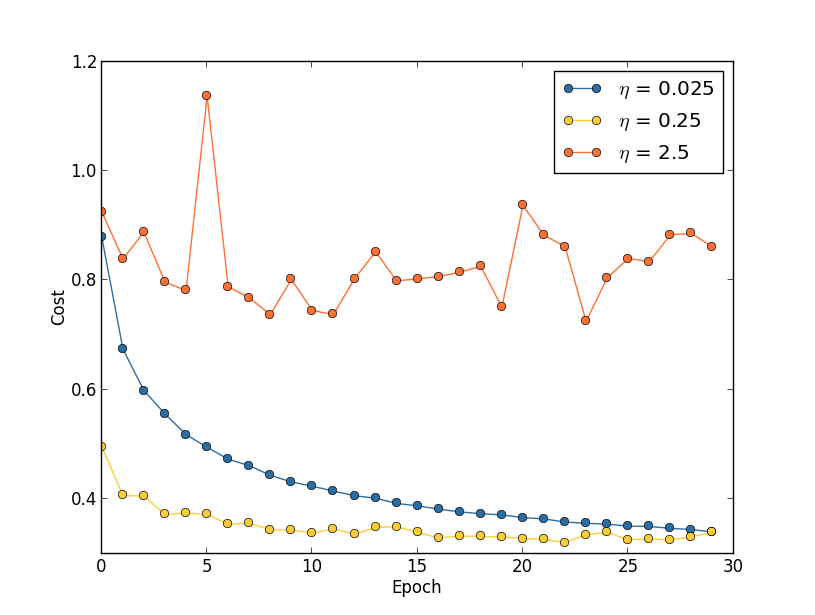
\includegraphics[width=0.867\textwidth]{images/multiple_eta.png}
\end{center}

\noindent 当 $\eta = 0.025$ 时，代价平滑下降直到最后一个轮次. 当 $\eta = 0.25$ 时，代价最初下降，但在大约 $20$ 个轮次后接近饱和，此后大部分变化只是微小且看似随机的振荡. 最后，当 $\eta = 2.5$ 时，代价从一开始就产生大幅振荡. 要理解振荡的原因，回想一下随机梯度下降应该引导我们逐渐下降到代价函数的一个谷底，

\begin{center}
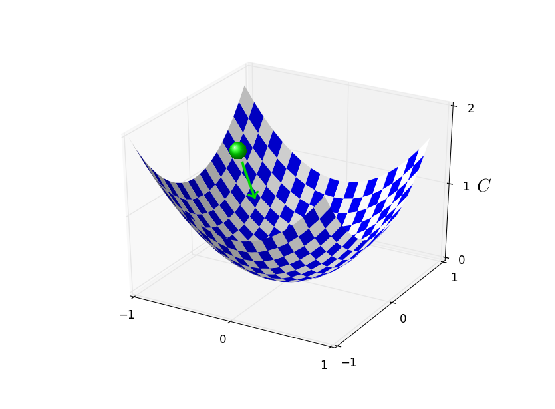
\includegraphics[width=0.9\textwidth]{images/tikz33.png}
\end{center}
\noindent 然而，如果 $\eta$ 太大，那么步长会大到实际上可能越过最小值，反而导致算法从谷底爬出来. 这很可能*\footnote{这个图景很有帮助，但它旨在作为可能发生情况的直觉性说明，而不是完整详尽的解释. 简而言之，更完整的解释如下：梯度下降使用代价函数的一阶近似来指导如何降低代价. 对于较大的 $\eta$，代价函数中的高阶项变得更加重要，并可能主导行为，导致梯度下降失效. 当我们接近代价函数的极小值和准极小值时，这种情况尤其可能发生，因为在这些点附近梯度变得很小，使得高阶项更容易主导行为.}就是当 $\eta = 2.5$ 时代价发生振荡的原因. 当我们选择 $\eta = 0.25$ 时，初始步骤确实将我们带向代价函数的极小值，只有当我们接近该极小值时，才开始受到过冲问题的影响. 而当我们选择 $\eta = 0.025$ 时，在前 $30$ 轮次中我们完全不会受到这个问题的影响. 当然，选择如此小的 $\eta$ 会带来另一个问题，即它会减慢随机梯度下降. 一个更好的方法是从 $\eta = 0.25$ 开始，训练 $20$ 轮次，然后切换到 $\eta = 0.025$. 我们稍后会讨论这种可变学习率日程\label{term:58}. 不过现在，让我们先专注于如何为学习率 $\eta$ 找到一个好的单一取值.

有了这个图景，我们可以按如下方式设定 $\eta$. 首先，我们估计 $\eta$ 的阈值，即训练数据上的代价立即开始下降而非振荡或上升的那个值. 这个估计不需要太精确. 你可以从 $\eta = 0.01$ 开始来估计数量级. 如果代价在前几轮次中下降，那么你应该依次尝试 $\eta = 0.1, 1.0, \ldots$，直到你找到一个 $\eta$ 值，使得代价在前几轮次中振荡或上升. 反之，如果在 $\eta = 0.01$ 时代价在前几轮次中振荡或上升，那么尝试 $\eta = 0.001, 0.0001, \ldots$，直到你找到一个 $\eta$ 值，使得代价在前几轮次中下降. 按照这个过程，我们将得到 $\eta$ 阈值的一个数量级估计. 你可以选择性地细化你的估计，找出代价在前几轮次中下降的最大 $\eta$ 值，比如 $\eta = 0.5$ 或 $\eta = 0.2$（这不需要非常精确）. 这样我们就得到了 $\eta$ 阈值的一个估计.

显然，你实际使用的 $\eta$ 值不应大于阈值. 事实上，如果 $\eta$ 的值要在许多轮次中保持可用，那么你可能希望使用一个更小的 $\eta$ 值，比如比阈值低两倍. 这样的选择通常能让你训练许多轮次，而不会导致学习速度过于缓慢.

在 MNIST 数据的情况下，遵循这一策略可以得到 $\eta$ 阈值的数量级估计为 $0.1$. 经过进一步细化，我们得到阈值 $\eta = 0.5$. 按照上述处方，这建议使用 $\eta = 0.25$ 作为我们的学习率取值. 事实上，我发现使用 $\eta = 0.5$ 在 $30$ 轮次中效果足够好，以至于大多数情况下我都不担心使用更低的 $\eta$ 值.

这一切看起来相当直接. 然而，使用训练代价来选择 $\eta$ 似乎与我在本节前面所说的相矛盾，即我们会通过使用留出的验证数据评估性能来选择超参数. 事实上，我们将使用验证准确率来选择正则化超参数、小批量大小以及网络参数（如层数和隐藏神经元数量等）. 为什么对学习率要区别对待呢？坦率地说，这个选择是我个人的审美偏好，也许有些特立独行. 理由是其他超参数旨在提高测试集上的最终分类准确率，因此基于验证准确率来选择它们是合理的. 然而，学习率只是附带地影响最终分类准确率. 它的主要目的实际上是控制梯度下降中的步长，而监控训练代价是检测步长是否过大的最佳方式. 话虽如此，这确实是一种个人审美偏好. 在学习早期，训练代价通常只在验证准确率提高时才会下降，因此实践中使用哪种标准不太可能产生太大差异.\textbf{使用提前停止来确定训练轮次数量：}正如我们在本章前面所讨论的，提前停止意味着在每个轮次结束时，我们应该计算验证数据上的分类准确率. 当它不再提高时，就终止. 这使得设置轮次数量变得非常简单. 特别是，这意味着我们不需要担心显式地弄清楚轮次数量如何依赖于其他超参数. 相反，这是自动处理的. 此外，提前停止还能自动防止我们过拟合. 这当然是一件好事，不过在实验的早期阶段，关闭提前停止可能是有帮助的，这样你可以看到任何过拟合的迹象，并利用它来指导你的正则化方法.

要实现提前停止，我们需要更精确地说明分类准确率停止提高意味着什么. 正如我们所看到的，准确率可能会大幅波动，即使整体趋势是提高的. 如果我们在准确率第一次下降时就停止，那么我们几乎肯定会在还有更多改进空间时就停止. 一个更好的规则是，如果最佳分类准确率在相当长一段时间内没有提高，就终止. 例如，假设我们正在做 MNIST. 那么我们可以选择在分类准确率在过去十轮次中没有提高时终止. 这确保了我们不会因为训练中的坏运气而停止得太早，同时也确保我们不会永远等待一个永远不会到来的改进.

这个“十轮次无改进”规则对于 MNIST 的初步探索是好的. 然而，网络有时会在某个特定分类准确率附近停滞相当长一段时间，然后又开始提高. 如果你试图获得真正好的性能，“十轮次无改进”规则可能在停止方面过于激进. 在这种情况下，我建议在初步实验中使用“十轮次无改进”规则，随着你更好地理解网络的训练方式，逐渐采用更宽松的规则：“二十轮次无改进”、“五十轮次无改进”等等. 当然，这引入了一个新的需要优化的超参数！然而在实践中，通常很容易设置这个超参数来获得相当好的结果. 同样，对于 MNIST 以外的问题，“十轮次无改进”规则可能过于激进或远远不够激进，这取决于问题的细节. 然而，通过一点实验，通常很容易找到一个相当好的提前停止策略.

到目前为止，我们在 MNIST 实验中还没有使用提前停止. 原因是我们一直在进行大量不同学习方法的比较. 对于这样的比较，在每个情况下使用相同的轮次数量是有帮助的. 然而，修改 \texttt{network2.py} 来实现提前停止是非常值得的：

\begin{exerciseBox}{习题}

\begin{itemize}

\item 修改 \texttt{network2.py}，使其使用“$n$ 轮次无改进”策略实现提前停止，其中 $n$ 是一个可以设置的参数.

\item 你能想到一个\emph{不同于}“$n$ 轮次无改进”的提前停止规则吗？理想情况下，该规则应该在获得高验证准确率和不过度训练之间取得折中. 将你的规则添加到 \texttt{network2.py} 中，并运行三个实验，将验证准确率和训练轮次数量与“$10$ 轮次无改进”进行比较.

\end{itemize}

\textbf{学习率日程：}我们一直保持学习率 $\eta$ 不变. 然而，变化学习率通常是有利的. 在学习过程的早期，权重很可能是严重错误的. 因此，最好使用较大的学习率，使权重快速变化. 之后，当我们对权重进行更精细的调整时，可以降低学习率.

我们应该如何设置学习率日程？有许多可能的方法. 一种自然的方法是使用与提前停止相同的基本思想. 其思想是保持学习率不变，直到验证准确率开始变差. 然后将学习率降低某个量，比如两倍或十倍. 我们重复这个过程多次，直到学习率比初始值低 $1,024$（或 $1,000$）倍. 然后我们终止.

可变学习日程可以提高性能，但它也打开了学习日程可能选择的世界. 这些选择可能令人头疼——你可以永远花时间试图优化你的学习日程. 对于初步实验，我的建议是使用单一的恒定学习率值. 这会给你一个很好的初步近似. 之后，如果你想从网络中获得最佳性能，值得按照我所描述的思路尝试学习日程*\footnote{一篇可读的近期论文展示了可变学习率在攻克 MNIST 时的优势，即 Deep, Big, Simple Neural Nets Excel on Handwritten Digit Recognition，作者为 Dan Claudiu Cireșan、Ueli Meier、Luca Maria Gambardella 和 Jürgen Schmidhuber（2010）.}.

\end{exerciseBox}

\begin{exerciseBox}{练习}

\begin{itemize}

\item 修改 \texttt{network2.py}，使其实现一个学习日程：每当验证准确率满足“$10$ 轮次无改进”规则时将学习率减半；并在学习率降至其原始值的 $1/128$ 时终止.

\end{itemize}

\textbf{正则化参数 $\lambda$：}我建议最初从无正则化（$\lambda = 0.0$）开始，并如上所述确定 $\eta$ 的值. 使用该 $\eta$ 选择，我们可以然后使用验证数据来选择 $\lambda$ 的一个好的值. 从试验 $\lambda = 1.0$*\footnote{我没有好的有原则的理由来使用这个作为起始值. 如果有人知道关于 $\lambda$ 从哪里开始的有原则的讨论，我将很感激听到它（mn@michaelnielsen.org）.}开始，然后根据需要以 $10$ 的倍数增加或减少，以提高验证数据上的性能. 一旦你找到了一个好的数量级，你就可以微调你的 $\lambda$ 值. 完成后，你应该返回并再次重新优化 $\eta$.

\end{exerciseBox}

\begin{exerciseBox}{练习}

\begin{itemize}

\item 使用梯度下降来尝试学习 $\lambda$ 和 $\eta$ 等超参数的好值是很有诱惑力的. 你能想到使用梯度下降来确定 $\lambda$ 的一个障碍吗？你能想到使用梯度下降来确定 $\eta$ 的一个障碍吗？

\end{itemize}

\textbf{我在本书前面是如何选择超参数的：}如果你使用本节的建议，你会发现你得到的 $\eta$ 和 $\lambda$ 值并不总是与我在本书前面使用的值完全匹配. 原因是本书有叙事上的限制，有时使得优化超参数变得不切实际. 想想我们做过的所有不同学习方法的比较，例如，比较二次代价函数和交叉熵代价函数，比较新旧权重初始化方法，在有和没有正则化的情况下运行，等等. 为了使这样的比较有意义，我通常试图在比较的方法之间保持超参数不变（或以适当的方式缩放它们）. 当然，没有理由相同的超参数对所有不同的学习方法都是最优的，所以我使用的超参数是一种折中.

作为这种折中的替代方案，我本可以尝试为每一种学习方法最大限度地优化超参数. 原则上，那将是一种更好、更公平的方法，因为那样我们就能看到每种学习方法的最佳表现. 然而，我们沿着这些思路做了几十次比较，实践中我发现计算成本太高. 这就是为什么我采用了使用相当好（但不一定最优）的超参数选择的折中方案.\textbf{小批量大小：}我们应该如何设置小批量大小？为了回答这个问题，让我们首先假设我们正在做在线学习，即我们使用的小批量大小为 $1$.

关于在线学习的明显担忧是，使用仅包含单个训练样本的小批量会导致我们的梯度估计出现显著误差. 然而事实上，这些误差结果证明并不是什么大问题. 原因是个体梯度估计不需要非常精确. 我们所需要的只是一个足够精确的估计，使我们的代价函数倾向于持续下降. 这就好像你试图到达北磁极，但有一个不稳定的指南针，每次你看它时都偏离 10-20 度. 只要你经常停下来检查指南针，并且指南针平均而言方向正确，你最终就能顺利到达北磁极.

基于这个论证，听起来我们应该使用在线学习. 事实上，情况结果证明比这更复杂. 在上一章的一个习题中，我指出可以使用矩阵技术同时计算小批量中\emph{所有}样本的梯度更新，而不是对它们进行循环. 取决于你的硬件和线性代数库的细节，这可以使计算（例如）大小为 $100$ 的小批量的梯度估计比通过分别循环 $100$ 个训练样本来计算小批量梯度估计快相当多. 它可能只需要（比如说）$50$ 倍的时间，而不是 $100$ 倍的时间.

现在，起初这似乎对我们帮助不大. 对于大小为 $100$ 的小批量，权重的学习规则看起来像：

\begin{equation}
w \rightarrow w' = w-\eta \frac{1}{100} \sum_x \nabla C_x,
\tag{100}
\end{equation}

\noindent 其中求和是对小批量中的训练样本进行的. 这对比于

\begin{equation}
w \rightarrow w' = w-\eta \nabla C_x
\tag{101}
\end{equation}

\noindent 在线学习的情况. 即使做小批量更新只需要 $50$ 倍的时间，看起来仍然可能更好地做在线学习，因为我们会更新得频繁得多. 然而，假设在小批量情况下我们将学习率增加 $100$ 倍，那么更新规则变为

\begin{equation}
w \rightarrow w' = w-\eta \sum_x \nabla C_x.
\tag{102}
\end{equation}

\noindent 这很像以学习率 $\eta$ 做 $100$ 次独立的在线学习. 但它只需要做单次在线学习 $50$ 倍的时间. 当然，它与 $100$ 次在线学习并不完全相同，因为在小批量中所有 $\nabla C_x$ 都是在同一组权重下评估的，而不是在线学习情况下发生的累积学习. 尽管如此，使用更大的小批量似乎明显有可能加快速度.

考虑到这些因素，选择最佳小批量大小是一种折中. 太小，你就无法充分利用为快速硬件优化的优秀矩阵库的优势. 太大，你就只是没有足够频繁地更新权重. 你需要的是选择一个折中值，使学习速度最大化. 幸运的是，速度最大化时的小批量大小选择相对独立于其他超参数（除了整体架构），所以你不需要先优化那些超参数就能找到好的小批量大小. 因此，方法是使用一些可接受的（但不一定最优的）其他超参数值，然后试验若干不同的小批量大小，如上所述缩放 $\eta$. 绘制验证准确率与\emph{时间}（即实际经过的时间，而不是轮次！）的关系，并选择能给你带来最快性能提升的小批量大小. 选定了小批量大小后，你就可以继续优化其他超参数了.

当然，正如你无疑已经意识到的，我在我们的工作中没有做这种优化. 事实上，我们的实现根本没有使用更快的小批量更新方法. 在几乎所有例子中，我只是简单地使用了小批量大小 $10$，没有评论或解释. 因此，我们本可以通过减小小批量大小来加速学习. 我没有这样做，部分是因为我想说明使用大于 $1$ 的小批量，部分是因为我的初步实验表明加速会相当有限. 然而，在实际实现中，我们肯定会实现更快的小批量更新方法，然后努力优化小批量大小，以最大化我们的整体速度.\textbf{自动化技术：}我一直在描述这些启发式方法，就好像你在手动优化超参数. 手动优化是建立对神经网络行为直觉的好方法. 然而，不出所料，在自动化这个过程方面已经做了大量工作. 一种常见的技术是\emph{网格搜索}，它在超参数空间中系统地搜索一个网格. 关于网格搜索的成就和局限性的综述（附有易于实现的替代方案的建议）可以在 James Bergstra 和 Yoshua Bengio 的 2012 年论文*\footnote{Random search for hyper-parameter optimization，作者为 James Bergstra 和 Yoshua Bengio（2012）.}中找到. 许多更复杂的方法也被提出了. 我不会在这里综述所有这些工作，但想提到一篇特别有前景的 2012 年论文，它使用贝叶斯方法来自动优化超参数*\footnote{Practical Bayesian optimization of machine learning algorithms，作者为 Jasper Snoek、Hugo Larochelle 和 Ryan Adams.}. 该论文的代码是公开可用的，并已被其他研究人员取得了一些成功.\textbf{总结：}遵循我所描述的经验法则不会从你的神经网络中获得绝对最好的可能结果. 但它很可能会给你一个好的开始和进一步改进的基础. 特别是，我基本上是独立地讨论超参数的. 实践中，超参数之间存在关系. 你可能会试验 $\eta$，觉得你已经把它调得恰到好处，然后开始优化 $\lambda$，却发现它打乱了你对 $\eta$ 的优化. 实践中，来回反复调整，逐渐逼近好的值是有帮助的. 最重要的是，记住我所描述的启发式方法是经验法则，不是一成不变的规则. 你应该留意事情不奏效的迹象，并愿意进行实验. 特别是，这意味着仔细监控你的网络行为，尤其是验证准确率.

选择超参数的困难因以下事实而加剧：关于如何选择超参数的知识广泛分散在许多研究论文和软件程序中，而且往往只存在于个别实践者的头脑中. 有许许多多的论文提出了（有时相互矛盾的）关于如何进行的建议. 然而，有几篇特别有用的论文综合并提炼了这些知识中的大部分.Yoshua Bengio 有一篇 2012 年的论文*\footnote{Practical recommendations for gradient-based training of deep architectures，作者为 Yoshua Bengio（2012）.}，给出了一些使用反向传播和梯度下降来训练神经网络（包括深度神经网络）的实用建议.Bengio 比我更详细地讨论了许多问题，包括如何进行更系统的超参数搜索. 另一篇好论文是 Yann LeCun、Léon Bottou、Genevieve Orr 和 Klaus-Robert Müller 的 1998 年论文*\footnote{Efficient BackProp，作者为 Yann LeCun、Léon Bottou、Genevieve Orr 和 Klaus-Robert Müller（1998）.}. 这两篇论文都出现在一本极其有用的 2012 年书籍中，该书收集了神经网络中常用的许多技巧*\footnote{Neural Networks: Tricks of the Trade，由 Grégoire Montavon、Geneviève Orr 和 Klaus-Robert Müller 编辑.}. 这本书很贵，但许多文章已被各自作者放到网上，想必得到了出版商的许可，可以使用搜索引擎找到.

当你阅读这些文章时，尤其是当你进行自己的实验时，有一件事变得很清楚：超参数优化从来不是一个完全解决的问题. 总还有另一个技巧可以尝试来提高性能. 作家中有一句常说的话：书永远不会完成，只会被放弃. 神经网络优化也是如此：超参数空间如此之大，以至于人永远不会真正完成优化，只会将网络遗留给后世. 所以你的目标应该是开发一种工作流程，使你能够快速地在优化上做得相当好，同时保留灵活性，以便在重要时尝试更详细的优化.

设置超参数的挑战使一些人抱怨神经网络与其他机器学习技术相比需要大量工作. 我听过以下抱怨的许多变体：``是的，一个调好的神经网络可能在该问题上获得最佳性能. 但另一方面，我可以尝试随机森林 [或 SVM 或$\ldots$ 插入你自己喜欢的技术]，它就能直接工作. 我没有时间弄清楚恰好正确的神经网络.''当然，从实际角度来看，拥有易于应用的技术是好的. 当你刚刚开始一个问题，而且机器学习是否能帮助解决这个问题可能还不明显时，这一点尤其正确. 另一方面，如果获得最优性能很重要，那么你可能需要尝试需要更多专业知识的方案. 虽然机器学习总是很简单就好了，但没有\emph{先验}理由表明它应该是轻而易举的.

\end{exerciseBox}
\sectionTitle{其他技术}{其他技术}

本章中发展的每一项技术本身都值得了解，但这并不是我解释它们的唯一原因. 更重要的目的是让你熟悉神经网络中可能出现的一些问题，以及一种有助于克服这些问题的分析风格. 从某种意义上说，我们一直在学习如何思考神经网络. 在本章的剩余部分，我将简要概述另外几项技术. 这些概述不如之前的讨论那样深入，但应当能让你感受到可用于神经网络的技术之多样.
\subsectionTitle{随机梯度下降的变体}{随机梯度下降的变体}

通过反向传播实现的随机梯度下降在解决 MNIST 数字分类问题上一直表现良好. 然而，还有许多其他优化代价函数的方法，有时这些其他方法能提供优于小批量随机梯度下降的性能. 在本节中，我概述两种这样的方法： Hessian 方法和动量方法. \textbf{Hessian 方法：} 为了开始我们的讨论，暂且把神经网络放在一边会有所帮助. 相反，我们只考虑最小化代价函数 $C$ 的抽象问题， $C$ 是许多变量的函数， $w = w_1, w_2, \ldots$，所以 $C = C(w)$. 根据泰勒定理，代价函数可以在点 $w$ 附近近似为

\begin{align}
C(w+\Delta w) &= C(w) + \sum_j \frac{\partial C}{\partial w_j} \Delta w_j \nonumber \\ & & + \frac{1}{2} \sum_{jk} \Delta w_j \frac{\partial^2 C}{\partial w_j \partial w_k} \Delta w_k + \ldots \tag{103}
\end{align}

\noindent 我们可以更紧凑地将其重写为

\begin{equation}
C(w+\Delta w) = C(w) + \nabla C \cdot \Delta w + \frac{1}{2} \Delta w^T H \Delta w + \ldots,
\tag{104}
\end{equation}

\noindent 其中 $\nabla C$ 是通常的梯度向量， $H$ 是一个称为 \emph{Hessian 矩阵}的矩阵，其 $jk$ 项为 $\partial^2 C / \partial w_j \partial w_k$. 假设我们通过丢弃上面由 $\ldots$ 表示的高阶项来近似 $C$,

\begin{equation}
C(w+\Delta w) \approx C(w) + \nabla C \cdot \Delta w + \frac{1}{2} \Delta w^T H \Delta w.
\tag{105}
\end{equation}

\noindent 使用微积分我们可以证明，通过选择以下式子，右侧的表达式可以被最小化*\footnote{严格来说，要使其成为最小值而不仅仅是极值，我们需要假设 Hessian 矩阵是正定的. 直观地说，这意味着函数 $C$ 局部看起来像一个山谷，而不是山峰或鞍点.}

\begin{equation}
\Delta w = -H^{-1} \nabla C.
\tag{106}
\end{equation}

\noindent 只要 (105)

\begin{align*}
C(w+\Delta w) \approx C(w) + \nabla C \cdot \Delta w + \frac{1}{2} \Delta w^T H \Delta w \nonumber
\end{align*}

\noindent 是代价函数的一个良好近似表达式，那么我们可以预期从点 $w$ 移动到 $w+\Delta w = w-H^{-1} \nabla C$ 应该会显著减小代价函数. 这提示了一个可能的最小化代价的算法：

\begin{itemize}

\item 选择一个起始点 $w$.

\item 将 $w$ 更新为新点 $w' = w-H^{-1} \nabla C$，其中 Hessian $H$ 和 $\nabla C$ 在 $w$ 处计算.

\item 将 $w'$ 更新为新点 $w{'}{'} = w'-H'^{-1} \nabla' C$，其中 Hessian $H'$ 和 $\nabla' C$ 在 $w'$ 处计算.

\item $\ldots$

\end{itemize}

在实践中， (105)

\begin{align*}
C(w+\Delta w) \approx C(w) + \nabla C \cdot \Delta w + \frac{1}{2} \Delta w^T H \Delta w \nonumber
\end{align*}

\noindent 只是一个近似，采取较小的步长会更好. 我们通过反复将 $w$ 改变 $\Delta w = -\eta H^{-1} \nabla C$ 来实现这一点，其中 $\eta$ 被称为学习率.

这种最小化代价函数的方法被称为 \emph{Hessian 方法}或 \emph{Hessian 优化}. 有理论和实证结果表明， Hessian 方法比标准梯度下降以更少的步数收敛到最小值. 特别是，通过纳入关于代价函数二阶变化的信息， Hessian 方法有可能避免梯度下降中可能出现的许多病态情况. 此外，还有可以用于计算 Hessian 的反向传播算法版本.

如果 Hessian 优化如此出色，为什么我们不在神经网络中使用它呢？不幸的是，尽管它有许多理想的特性，但它有一个非常不受欢迎的特性：它在实践中非常难以应用. 部分问题在于 Hessian 矩阵的规模巨大. 假设你有一个具有 $10^7$ 个权重和偏置的神经网络. 那么相应的 Hessian 矩阵将包含 $10^7 \times 10^7 = 10^{14}$ 个元素. 那可是很多元素！这使得在实践中计算 $H^{-1} \nabla C$ 极其困难. 然而，这并不意味着理解它没有用. 事实上，有许多梯度下降的变体受到 Hessian 优化的启发，但避免了矩阵过大的问题. 让我们来看一种这样的技术：基于动量的梯度下降. \textbf{基于动量的梯度下降：} 直观地说， Hessian 优化的优势在于它不仅纳入了关于梯度的信息，还纳入了关于梯度如何变化的信息. 基于动量的梯度下降基于类似的直觉，但避免了大型的二阶导数矩阵. 要理解动量技术，回想一下我们最初关于梯度下降的图景，其中我们考虑了一个滚入山谷的球. 当时，我们观察到梯度下降尽管名字如此，但只是粗略地类似于球落入谷底. 动量技术以两种方式修改梯度下降，使其更接近物理图景. 首先，它为我们试图优化的参数引入了``速度''的概念. 梯度作用于改变速度，而不是(直接)改变``位置''，这与物理力改变速度，仅间接影响位置非常相似. 其次，动量方法引入了一种摩擦力项，它倾向于逐渐减小速度.

让我们给出更精确的数学描述. 我们引入速度变量 $v = v_1, v_2, \ldots$，每个对应于相应的 $w_j$ 变量*\footnote{在神经网络中， $w_j$ 变量当然会包括所有权重和偏置.}. 然后我们将梯度下降更新规则 $w \rightarrow w'= w-\eta \nabla C$ 替换为

\begin{align}
v &\rightarrow v' = \mu v - \eta \nabla C \tag{107} \\ w &\rightarrow w' = w+v'. \tag{108}
\end{align}

\noindent 在这些方程中， $\mu$ 是一个超参数，控制系统中的阻尼或摩擦量. 要理解这些方程的含义，首先考虑 $\mu = 1$ 的情况会有所帮助，这对应于没有摩擦. 在这种情况下，检查方程表明``力'' $\nabla C$ 现在正在修改速度 $v$，而速度控制着 $w$ 的变化率. 直观地说，我们通过反复向速度添加梯度项来积累速度. 这意味着如果梯度在几轮学习中(大致)沿同一方向，我们就可以在该方向上积累相当多的动量. 例如，想想如果我们正沿着斜坡直线下降会发生什么：

\begin{center}
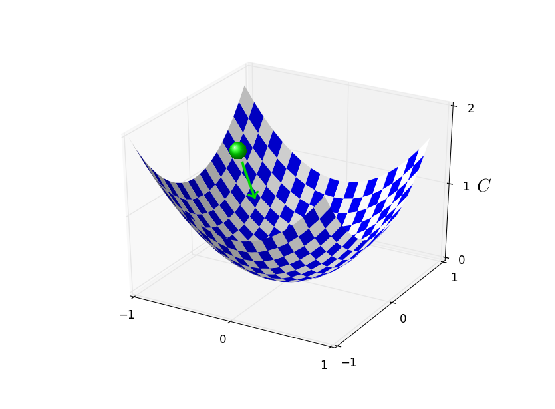
\includegraphics[width=0.9\textwidth]{images/tikz34.png}
\end{center}

\noindent 每走一步，沿斜坡向下的速度就会增大，因此我们越来越快地移动到谷底. 这可以使动量技术比标准梯度下降快得多. 当然，一个问题是，一旦我们到达谷底，我们就会冲过头. 或者，如果梯度变化很快，那么我们可能会发现自己朝着错误的方向移动. 这就是 (107) 中 $\mu$ 超参数的原因

\begin{align*}
v &\rightarrow v' = \mu v - \eta \nabla C \nonumber
\end{align*}

\noindent. 我之前说过 $\mu$ 控制系统中的摩擦量；更精确地说，你应该将 $1-\mu$ 视为系统中的摩擦量. 当 $\mu = 1$ 时，正如我们所看到的，没有摩擦，速度完全由梯度 $\nabla C$ 驱动. 相反，当 $\mu = 0$ 时，有很大的摩擦，速度无法积累，方程 (107)

\begin{align*}
v &\rightarrow v' = \mu v - \eta \nabla C \nonumber
\end{align*}

\noindent 和 (108)

\begin{align*}
w &\rightarrow w' = w+v' \nonumber
\end{align*}

\noindent 简化为通常的梯度下降方程 $w \rightarrow w'=w-\eta \nabla C$. 在实践中，使用介于 $0$ 和 $1$ 之间的 $\mu$ 值可以给我们带来能够积累速度的大部分好处，而不会导致冲过头. 我们可以使用留出的验证数据来选择这样的 $\mu$ 值，就像我们选择 $\eta$ 和 $\lambda$ 一样.

到目前为止，我一直避免给超参数 $\mu$ 命名. 原因是 $\mu$ 的标准名称选择得很糟糕：它被称为 \emph{动量系数}. 这可能会引起混淆，因为 $\mu$ 与物理学中的动量概念完全不同. 相反，它与摩擦的关系更为密切. 然而，动量系数这个术语被广泛使用，所以我们将继续使用它.

动量技术的一个好处是，修改梯度下降的实现以纳入动量几乎不需要任何工作. 我们仍然可以使用反向传播来计算梯度，就像以前一样，并使用诸如随机选择小批量样本之类的想法. 通过这种方式，我们可以获得 Hessian 方法的一些优势，利用关于梯度如何变化的信息. 但这样做没有缺点，并且只需要对我们的代码进行微小的修改. 在实践中，动量技术被普遍使用，并且经常加速学习.

\begin{exerciseBox}{练习}

\begin{itemize}

\item 如果我们在动量技术中使用 $\mu > 1$ 会出什么问题？

\item 如果我们在动量技术中使用 $\mu < 0$ 会出什么问题？

\end{itemize}

\end{exerciseBox}

\begin{exerciseBox}{习题}

\begin{itemize}

\item 将基于动量的随机梯度下降添加到 \texttt{network2.py} 中.

\end{itemize}

\textbf{其他最小化代价函数的方法：} 许多其他最小化代价函数的方法已经被开发出来，对于哪种方法最好并没有普遍的共识. 当你更深入地研究神经网络时，值得深入研究其他技术，理解它们的工作原理，优缺点，以及如何在实际中应用它们. 我之前提到的一篇论文*\footnote{Efficient BackProp, by Yann LeCun, Léon Bottou, Genevieve Orr and Klaus-Robert Müller (1998).} 介绍并比较了其中几种技术，包括共轭梯度下降和 BFGS 方法(另见密切相关的有限内存 BFGS 方法，称为 L-BFGS). 另一种最近显示出有希望结果的技术*\footnote{See, for example, On the importance of initialization and momentum in deep learning, by Ilya Sutskever, James Martens, George Dahl, and Geoffrey Hinton (2012).} 是 Nesterov 加速梯度技术，它改进了动量技术. 然而，对于许多问题，普通的随机梯度下降效果很好，特别是如果使用动量，因此在本书的剩余部分我们将坚持使用随机梯度下降.

\end{exerciseBox}
\subsectionTitle{人工神经元的其他模型}{人工神经元的其他模型}

到目前为止，我们一直使用 S 型神经元来构建神经网络. 原则上，由 S 型神经元构成的网络可以计算任意函数. 然而在实践中，使用其他模型神经元构建的网络有时会优于 S 型网络. 根据应用的不同，基于这些替代模型的网络可能学习得更快、对测试数据泛化得更好，或者两者兼而有之. 让我介绍几种替代模型神经元，让你感受一下一些常用变体的风格.

也许最简单的变体是 tanh（读作 ``tanch''）神经元，它用双曲正切函数取代了 S 型函数. 一个 tanh 神经元在输入 $x$、权重向量 $w$ 和偏置 $b$ 下的输出由下式给出

\begin{equation}
\tanh(w \cdot x+b),
\tag{109}
\end{equation}

\noindent 其中 $\tanh$ 当然就是双曲正切函数. 事实证明，它与 S 型神经元密切相关. 要看出这一点，回想一下 $\tanh$ 函数的定义是

\begin{equation}
\tanh(z) \equiv \frac{e^z-e^{-z}}{e^z+e^{-z}}.
\tag{110}
\end{equation}

\noindent 稍作代数运算便可轻易验证

\begin{equation}
\sigma(z) = \frac{1+\tanh(z/2)}{2},
\tag{111}
\end{equation}

\noindent 也就是说，$\tanh$ 只不过是 S 型函数的一个重新缩放版本. 我们也可以从图形上看出 $\tanh$ 函数与 S 型函数具有相同的形状.tanh 神经元与 S 型神经元的一个区别在于，tanh 神经元的输出范围是 -1 到 1，而不是 0 到 1. 这意味着如果你要构建一个基于 tanh 神经元的网络，你可能需要以与 S 型网络略有不同的方式对你的输出（并且，根据应用的具体细节，可能还有你的输入）进行规范化\label{term:59}.

与 S 型神经元类似，tanh 神经元构成的网络原则上可以计算任意函数*\footnote{对于 tanh 神经元和 S 型神经元，以及下面讨论的修正线性神经元，这一说法都有一些技术上的注意事项. 不过，非正式地说，通常可以把神经网络理解为能够以任意精度近似任意函数.}，将输入映射到 -1 到 1 的范围. 此外，诸如反向传播和随机梯度下降之类的思想，应用于 tanh 神经元网络与应用于 S 型神经元网络一样容易.

\begin{exerciseBox}{练习}

\begin{itemize}

\item
证明方程 (111) 中的恒等式

\begin{align*}
\sigma(z) = \frac{1+\tanh(z/2)}{2} \nonumber
\end{align*}

.

\end{itemize}

你应该在网络中使用哪种类型的神经元，tanh 还是 S 型？\emph{先验地} 说，答案并不明显，说得委婉一点！然而，有理论论证和一些经验证据表明 tanh 有时表现更好*\footnote{例如，参见 Yann LeCun、Léon Bottou、Genevieve Orr 和 Klaus-Robert Müller (1998) 的 Efficient BackProp，以及 Xavier Glorot 和 Yoshua Bengio (2010) 的 Understanding the difficulty of training deep feedforward networks.}. 让我简要地介绍一下支持 tanh 神经元的其中一个理论论证的风格. 假设我们使用 S 型神经元，因此网络中所有的激活值都是正的. 让我们考虑输入到第 $l+1$ 层第 $j$ 个神经元的权重 $w^{l+1}_{jk}$. 反向传播的规则（见此处）告诉我们，相关的梯度将是 $a^l_k \delta^{l+1}_j$. 因为激活值是正的，这个梯度的符号将与 $\delta^{l+1}_j$ 的符号相同. 这意味着如果 $\delta^{l+1}_j$ 是正的，那么在梯度下降过程中 \emph{所有} 权重 $w^{l+1}_{jk}$ 都会减小，而如果 $\delta^{l+1}_j$ 是负的，那么在梯度下降过程中 \emph{所有} 权重 $w^{l+1}_{jk}$ 都会增大. 换句话说，连接到同一个神经元的所有权重必须要么一起增大，要么一起减小. 这是个问题，因为有些权重可能需要增大而另一些需要减小. 只有当某些输入激活值具有不同的符号时，这种情况才可能发生. 这提示我们用一种允许正负激活值的激活函数来取代 S 型函数，例如 $\tanh$. 事实上，因为 $\tanh$ 关于零对称，$\tanh(-z) = -\tanh(z)$，我们甚至可以期望，粗略地说，隐藏层中的激活值会在正负之间大致均衡. 这将有助于确保权重更新不会系统性地偏向某一个方向.

我们应该多认真地对待这个论证呢？虽然这个论证很有启发性，但它只是一种启发式推理，而不是 tanh 神经元优于 S 型神经元的严格证明. 也许 S 型神经元还有其他特性可以弥补这个问题？事实上，对于许多任务，经验上发现 tanh 相比 S 型神经元只能带来很小的性能提升，甚至没有提升. 不幸的是，对于任何特定的应用，我们还没有确定不移的规则来知道哪种神经元类型学习最快，或者给出最好的泛化性能.

S 型神经元的另一种变体是 \emph{修正线性神经元} 或 \emph{修正线性单元}. 一个修正线性单元在输入 $x$、权重向量 $w$ 和偏置 $b$ 下的输出由下式给出

\begin{equation}
\max(0, w \cdot x+b).
\tag{112}
\end{equation}

\noindent 从图形上看，修正函数 $\max(0, z)$ 看起来是这样的：显然，这类神经元与 S 型神经元和 tanh 神经元都相当不同. 然而，与 S 型神经元和 tanh 神经元一样，修正线性单元\label{term:60}可以用来计算任意函数，并且可以使用反向传播和随机梯度下降之类的思想来训练.

什么时候你应该使用修正线性单元而不是 S 型或 tanh 神经元？一些最近的图像识别工作*\footnote{例如，参见 Kevin Jarrett、Koray Kavukcuoglu、Marc'Aurelio Ranzato 和 Yann LeCun (2009) 的 What is the Best Multi-Stage Architecture for Object Recognition？，Xavier Glorot、Antoine Bordes 和 Yoshua Bengio (2011) 的 Deep Sparse Rectifier Neural Networks，以及 Alex Krizhevsky、Ilya Sutskever 和 Geoffrey Hinton (2012) 的 ImageNet Classification with Deep Convolutional Neural Networks. 请注意，这些论文补充了关于在使用修正线性单元的网络中如何设置输出层、代价函数和正则化的重要细节. 在这个简要的叙述中，我忽略了所有这些细节. 这些论文还更详细地讨论了使用修正线性单元的利弊. 另一篇信息丰富的论文是 Vinod Nair 和 Geoffrey Hinton (2010) 的 Rectified Linear Units Improve Restricted Boltzmann Machines，它展示了在一种稍有不同的神经网络方法中使用修正线性单元的好处.} 发现在网络的大部分中使用修正线性单元有相当大的好处. 然而，与 tanh 神经元一样，我们还没有真正深入地理解究竟何时修正线性单元更可取，以及为什么. 为了让你感受一下其中一些问题，回想一下 S 型神经元在饱和时会停止学习，即当它们的输出接近 $0$ 或 $1$ 时. 正如我们在本章中反复看到的，问题在于 $\sigma'$ 项会减小梯度，从而减慢学习速度.tanh 神经元在饱和时也会遇到类似的问题. 相比之下，增大修正线性单元的加权输入永远不会使它饱和，因此不存在相应的学习减速. 另一方面，当修正线性单元的加权输入为负时，梯度消失，因此该神经元完全停止学习. 这些只是众多问题中的两个，它们使得理解修正线性单元何时以及为何比 S 型或 tanh 神经元表现更好变得并非易事.

我在这里描绘了一幅充满不确定性的图景，强调我们还没有一个关于应该如何选择激活函数的坚实理论. 事实上，问题比我描述的还要困难，因为存在无穷多种可能的激活函数. 对于任何给定的问题，哪一种最好？哪一种会导致网络学习最快？哪一种会给出最高的测试准确率？令我惊讶的是，对这些问题真正深入和系统的研究竟然如此之少. 理想情况下，我们会有一个理论，详细地告诉我们如何选择（也许还可以动态修改）我们的激活函数. 另一方面，我们不应该让缺乏完整理论阻碍我们！我们手头已经有强大的工具，可以用这些工具取得很多进展. 在本书的剩余部分，我将继续使用 S 型神经元作为我们的首选神经元，因为它们功能强大，并且为关于神经网络的核心思想提供了具体的例证. 但请记住，这些同样的思想也可以应用于其他类型的神经元，而且这样做有时会有优势.

\end{exerciseBox}
\subsectionTitle{关于神经网络中的故事}{关于神经网络中的故事}

\begin{quote}
\emph{\textbf{问题：}你如何着手利用和研究那些几乎完全由经验而非数学支撑的机器学习技术？另外，在哪些情况下你注意到其中一些技术会失败？\textbf{回答：}你必须意识到我们的理论工具非常薄弱. 有时，我们对某项特定技术为何有效有着良好的数学直觉. 有时我们的直觉最终被证明是错误的 [...] 问题就变成了：我的方法在这个特定问题上表现如何，以及它在多大的问题集合上表现良好.- 与神经网络研究者 Yann LeCun 的问答}
\end{quote}

有一次，我参加了一个关于量子力学基础的会议，我注意到一个在我看来非常奇特的口头习惯：当演讲结束时，听众的提问常常以 ``我非常赞同你的观点，但是 [...]'' 开头. 量子基础并非我通常的领域，我之所以注意到这种提问方式，是因为在其他科学会议上，我很少或从未听到提问者表达对演讲者观点的赞同. 当时，我认为这种提问的普遍性表明量子基础领域几乎没有取得真正的进展，人们只是在原地打转. 后来，我意识到这个评价过于苛刻. 演讲者们正在与人类心智所面对过的一些最困难的问题作斗争. 当然进展缓慢！但即使他们并不总是有无可争辩的新进展可以报告，听取人们思考方式的最新动态仍然是有价值的.

你可能已经注意到本书中有一个类似于 ``我非常赞同 [...]'' 的口头习惯. 为了解释我们所看到的现象，我常常退回到说 ``启发式地讲，[...]''，或者 ``粗略地说，[...]''，然后接着用一个故事来解释某个现象或其他东西. 这些故事是合理的，但我所呈现的经验证据往往相当薄弱. 如果你翻阅研究文献，你会看到类似风格的故事出现在许多关于神经网络的研究论文中，往往只有薄弱的支持证据. 我们应该如何看待这样的故事？

在科学的许多领域——尤其是那些处理简单现象的领域——有可能为相当普遍的假设获得非常坚实、非常可靠的证据. 但在神经网络中，存在大量的参数和超参数，以及它们之间极其复杂的相互作用. 在如此极其复杂的系统中，要建立可靠的普遍陈述是极其困难的. 从完全普遍的意义上理解神经网络，是一个像量子基础一样考验人类心智极限的问题. 相反，我们常常只能满足于支持或反对某个普遍陈述的少数具体实例的证据. 结果，当新的证据出现时，那些陈述有时后来需要被修改或放弃.

看待这种情况的一种方式是，任何关于神经网络的启发式故事都带有一种隐含的挑战. 例如，考虑我之前引用的那个陈述，解释 dropout 为何有效*\footnote{摘自 Alex Krizhevsky、Ilya Sutskever 和 Geoffrey Hinton 的 ImageNet Classification with Deep Convolutional Neural Networks (2012).}：``这种技术减少了神经元之间复杂的共适应，因为一个神经元不能依赖于特定其他神经元的存在. 因此，它被迫学习更稳健的特征，这些特征在与许多不同的其他神经元随机子集结合时是有用的.'' 这是一个丰富、具有挑衅性的陈述，人们完全可以围绕剖析这个陈述来建立一个富有成果的研究项目，弄清楚其中哪些是真的，哪些是假的，哪些需要变化和完善. 事实上，现在已经有一个小型的研究产业，研究者们在调查 dropout（以及许多变体），试图理解它如何工作，以及它的局限是什么. 我们讨论过的许多启发式方法也是如此. 每个启发式方法不仅是一个（潜在的）解释，也是一个需要更详细地调查和理解的挑战.

当然，没有任何一个人有时间去深入调查所有这些启发式解释. 神经网络研究者群体要发展出一个真正强大的、基于证据的关于神经网络如何学习的理论，将需要几十年（或更长时间）. 这是否意味着你应该拒绝启发式解释，认为它们不严谨、证据不足？不！事实上，我们需要这样的启发式方法来启发和指导我们的思考. 这就像伟大的探索时代：早期的探险家有时是在某些重要方面错误的信念基础上进行探索（并做出新发现）的. 后来，随着我们填补了地理知识，那些错误被纠正了. 当你对某件事理解得很差时——就像探险家对地理的理解，以及我们今天对神经网络的理解——大胆探索比在思考的每一步都严格正确更为重要. 因此，你应该把这些故事视为关于如何思考神经网络的有用指南，同时保持对这些故事局限性的健康意识，并仔细追踪任何给定推理路线的证据究竟有多强. 换句话说，我们需要好的故事来帮助激励和启发我们，也需要严谨的深入研究来揭示事情的真相.

\chapter{神经网络可以计算任意函数的直观证明}
关于神经网络最引人注目的事实之一是它们可以计算任意函数. 也就是说，假设有人交给你一个复杂的、弯弯曲曲的函数 $f(x)$：无论这个函数是什么，都保证存在一个神经网络，使得对于每一个可能的输入 $x$，网络都会输出值 $f(x)$（或某个接近的近似值），例如：即使函数有多个输入 $f = f(x_1, \ldots, x_m)$ 和多个输出，这一结果仍然成立. 例如，这里有一个计算具有 $m = 3$ 个输入和 $n = 2$ 个输出的函数的网络：这一结果告诉我们，神经网络具有一种\emph{通用性}（universality）\label{term:61}. 无论我们想要计算什么函数，我们都知道存在一个可以完成这项工作的神经网络.

更重要的是，即使我们将网络限制为在输入和输出神经元之间只有单层中间层——即所谓的单隐藏层，这一通用性定理仍然成立. 因此，即使是非常简单的网络结构也可以极其强大.

通用性定理对于使用神经网络的人来说是众所周知的. 但它为什么成立却并不那么广为人知. 大多数可获得的解释都相当技术化. 例如，证明这一结果的原始论文之一*\footnote{Approximation by superpositions of a sigmoidal function, by George Cybenko (1989). The result was very much in the air at the time, and several groups proved closely related results. Cybenko's paper contains a useful discussion of much of that work. Another important early paper is Multilayer feedforward networks are universal approximators, by Kurt Hornik, Maxwell Stinchcombe, and Halbert White (1989). This paper uses the Stone-Weierstrass theorem to arrive at similar results.} 使用了 Hahn-Banach 定理、Riesz 表示定理以及一些傅里叶分析来证明. 如果你是一个数学家，这个论证并不难理解，但对大多数人来说并不那么容易. 这很遗憾，因为通用性的根本原因是简单而优美的.

在本章中，我将给出一个简单且主要是可视化的通用性定理解释. 我们将一步一步地梳理其背后的思想. 你将理解为什么神经网络可以计算任意函数. 你将理解这一结果的一些局限性. 并且你将理解这一结果与深度神经网络的关系.

要跟上本章的内容，你不需要读过本书前面的章节. 相反，本章的结构使其作为一篇自成一体的文章而令人愉快. 只要你具备一点关于神经网络的基本知识，你就应该能够跟上解释. 不过，我会偶尔提供指向前面材料的链接，以帮助填补你知识中的任何空白.

通用性定理在计算机科学中是司空见惯的，以至于我们有时会忘记它们有多么令人惊叹. 但值得提醒我们自己：计算任意函数的能力确实是非凡的. 你能想象到的几乎任何过程都可以被视为函数计算. 考虑根据一小段音乐样本说出这段音乐的名称的问题. 这可以被视为计算一个函数. 或者考虑将一段中文文本翻译成英文的问题. 同样，这可以被视为计算一个函数*\footnote{实际上，是计算众多函数之一，因为对于给定的文本片段，通常有许多可接受的翻译.}. 或者考虑拿一个 mp4 电影文件，生成电影情节的描述，以及对表演质量的讨论的问题. 同样，这可以被视为一种函数计算*\footnote{关于翻译以及存在许多可能函数的评论同样适用.}. 通用性意味着，原则上，神经网络可以完成所有这些事情以及更多.

当然，仅仅因为我们知道存在一个可以（比如说）将中文文本翻译成英文的神经网络，并不意味着我们有好的技术来构造甚至识别这样一个网络. 这一局限性也适用于诸如布尔电路等模型的传统通用性定理. 但是，正如我们在本书前面所看到的，神经网络拥有强大的学习函数算法. 学习算法 + 通用性的组合是一种有吸引力的混合. 到目前为止，本书一直专注于学习算法. 在本章中，我们专注于通用性，以及它意味着什么.
\sectionTitle{两点说明}{两点说明}

在解释通用性定理为何成立之前，我想先提两点关于``神经网络可以计算任意函数''这一非正式说法的说明.

第一，这并不意味着网络能够被用来\emph{精确}计算任意函数. 更确切地说，我们可以得到一个\emph{近似}，并且这个近似可以任意好. 通过增加隐藏神经元的数量，我们可以改进近似效果. 例如，之前我用三个隐藏神经元展示了一个计算某个函数 $f(x)$ 的网络. 对于大多数函数来说，使用三个隐藏神经元只能得到低质量的近似. 通过增加隐藏神经元的数量（比如增加到五个），我们通常可以得到更好的近似：而进一步增加隐藏神经元的数量，我们还能做得更好.

为了更精确地表述这一点，假设给定一个函数 $f(x)$，我们希望以某个期望的精度 $\epsilon > 0$ 来计算它. 保证是：通过使用足够多的隐藏神经元，我们总能找到一个神经网络，其输出 $g(x)$ 对所有输入 $x$ 都满足 $|g(x) - f(x)| < \epsilon$. 换句话说，对于每一个可能的输入，近似都能达到期望的精度.

第二点说明是，能够以所述方式被近似的函数类，是\emph{连续}函数. 如果一个函数是不连续的，即发生突然的、急剧的跳跃，那么一般而言就不可能用神经网络来近似. 这并不奇怪，因为我们的神经网络计算的是其输入的连续函数. 然而，即使我们真正想要计算的函数是不连续的，也常常存在一个足够好的连续近似. 如果是这样，那么我们就可以使用神经网络. 在实践中，这通常不是一个重要的限制.

总结起来，通用性定理更精确的表述是：具有单个隐藏层的神经网络可以被用来以任意期望的精度近似任意连续函数. 在本章中，我们实际上将证明这个结果的一个稍弱版本，使用的是两个隐藏层而不是一个. 在习题中，我将简要概述如何稍作调整，就能使这一解释适用于给出一个只使用单个隐藏层的证明.
\sectionTitle{单输入单输出的通用性}{单输入单输出的通用性}

为了理解通用性定理为何成立，让我们先来理解如何构造一个仅有一个输入和一个输出的神经网络来近似一个函数：事实证明，这正是通用性问题的核心. 一旦我们理解了这个特殊情况，将其推广到具有多个输入和多个输出的函数实际上就相当容易了.

为了深入理解如何构造一个计算 $f$ 的网络，让我们从一个仅包含单个隐藏层、具有两个隐藏神经元，以及一个包含单个输出神经元的输出层的网络开始：为了感受网络中各个组件是如何工作的，让我们关注上面的隐藏神经元. 在下面的图中，点击权重 $w$，并将鼠标向右拖动一点以增大 $w$. 你可以立即看到上面隐藏神经元所计算的函数如何变化：正如我们在本书前面所学到的，隐藏神经元所计算的是 $\sigma(wx + b)$，其中 $\sigma(z) \equiv 1/(1+e^{-z})$ 是 S 型函数. 到目前为止，我们频繁地使用了这种代数形式. 但对于通用性的证明，我们将完全忽略代数，转而通过操作和观察图中所示的形状来获得更多的洞见. 这不仅会让我们更好地感受正在发生的事情，还会给我们一个适用于 S 型函数以外的激活函数的通用性证明*\footnote{严格来说，我所采用的视觉方法并不是传统意义上所认为的证明. 但我相信，视觉方法比传统证明更能让人洞见结果为何成立. 当然，这种洞见才是证明的真正目的. 偶尔，我所呈现的推理中会有一些小缺口：在这些地方，我给出了一个看似合理但不太严格的视觉论证. 如果这让你感到困扰，那么就把它当作一个填补缺失步骤的挑战. 但不要忘记真正的目的：理解通用性定理为何成立.}.

为了开始这个证明，请尝试点击上图中的偏置 $b$，并向右拖动以增大它. 你会看到，随着偏置增大，图形向左移动，但其形状不变.

接下来，点击并向左拖动以减小偏置. 你会看到，随着偏置减小，图形向右移动，但同样，其形状不变.

接下来，将权重减小到大约 $2$ 或 $3$. 你会看到，随着权重减小，曲线变宽. 你可能还需要改变偏置，以使曲线保持在视野内.

最后，将权重增大到超过 $w = 100$. 随着你这样做，曲线变得更陡峭，直到最终开始看起来像一个阶梯函数. 尝试调整偏置，使阶梯出现在 $x = 0.3$ 附近. 下面的短片展示了你的结果应该是什么样子. 点击播放按钮来播放（或重播）视频：

\begin{movieNote}{create\_\allowbreak{}step\_\allowbreak{}function}
\end{movieNote}

\noindent 我们可以通过将权重增大到输出在非常好的近似下确实是一个阶梯函数，来大大简化我们的分析. 下面我绘制了当权重为 $w = 999$ 时上面隐藏神经元的输出. 请注意，这个图是静态的，你无法改变权重等参数.

实际上，使用阶梯函数比使用一般的 S 型函数要容易得多. 原因在于，在输出层中，我们将所有隐藏神经元的贡献相加. 分析一堆阶梯函数的和很容易，但推理当你把一堆 S 型曲线相加时会发生什么则要困难得多. 因此，假设我们的隐藏神经元输出阶梯函数会使事情容易得多. 更具体地说，我们通过将权重 $w$ 固定为某个非常大的值，然后通过修改偏置来设置阶梯的位置来做到这一点. 当然，将输出视为阶梯函数是一种近似，但这是一个非常好的近似，目前我们将把它视为精确的. 稍后我会回来讨论偏离这种近似的影响.

阶梯出现在 $x$ 的什么值处？换句话说，阶梯的位置如何依赖于权重和偏置？

为了回答这个问题，请尝试修改上图中的权重和偏置（你可能需要向上滚动一点）. 你能弄清楚阶梯的位置如何依赖于 $w$ 和 $b$ 吗？稍加努力，你应该能够说服自己，阶梯的位置与 $b$ \emph{成正比}，与 $w$ \emph{成反比}.

事实上，阶梯位于位置 $s = -b/w$，你可以通过修改下图中的权重和偏置来看到这一点：仅使用单个参数 $s$ 来描述隐藏神经元将大大简化我们的生活，$s$ 就是阶梯位置，$s = -b/w$. 尝试修改下图中的 $s$，以习惯新的参数化方式：如上所述，我们隐含地将输入的权重 $w$ 设置为某个很大的值——大到足以使阶梯函数成为一个非常好的近似. 我们可以很容易地将以这种方式参数化的神经元转换回传统模型，只需选择偏置 $b = -w s$.

到目前为止，我们一直关注的是仅上面隐藏神经元的输出. 让我们来看看整个网络的行为. 特别地，我们将假设隐藏神经元计算由阶梯点 $s_1$（上面的神经元）和 $s_2$（下面的神经元）参数化的阶梯函数. 它们将分别具有输出权重 $w_1$ 和 $w_2$. 这是网络：右边绘制的是来自隐藏层的\emph{加权输出} $w_1 a_1 + w_2 a_2$. 这里，$a_1$ 和 $a_2$ 分别是上面和下面隐藏神经元的输出*\footnote{顺便注意，整个网络的输出是 $\sigma(w_1 a_1+w_2 a_2 + b)$，其中 $b$ 是输出神经元的偏置. 显然，这与我们这里绘制的来自隐藏层的加权输出不同. 我们现在将专注于来自隐藏层的加权输出，稍后才会考虑它与整个网络输出的关系.}. 这些输出用 $a$ 表示，因为它们通常被称为神经元的\emph{激活值}.

尝试增大和减小上面隐藏神经元的阶梯点 $s_1$. 感受一下这如何改变来自隐藏层的加权输出. 特别值得理解的是当 $s_1$ 越过 $s_2$ 时会发生什么. 你会看到，当这种情况发生时，图形会改变形状，因为我们已经从上面隐藏神经元最先被激活的情况转变为下面隐藏神经元最先被激活的情况.

同样，尝试操作下面隐藏神经元的阶梯点 $s_2$，并感受一下这如何改变来自隐藏神经元的组合输出.

尝试增大和减小每个输出权重. 注意这如何重新缩放来自相应隐藏神经元的贡献. 当其中一个权重为零时会发生什么？

最后，尝试将 $w_1$ 设为 $0.8$，将 $w_2$ 设为 $-0.8$. 你会得到一个``凸起''函数，它从点 $s_1$ 开始，到点 $s_2$ 结束，高度为 $0.8$. 例如，加权输出可能看起来像这样：当然，我们可以重新缩放凸起使其具有任意高度. 让我们使用单个参数 $h$ 来表示高度. 为了减少杂乱，我还将移除``$s_1 = \ldots$''和``$w_1 = \ldots$''的标注.

尝试上下改变 $h$ 的值，看看凸起的高度如何变化. 尝试将高度改为负值，并观察会发生什么. 并尝试改变阶梯点，看看这如何改变凸起的形状.

顺便你会注意到，我们使用神经元的方式不仅可以从图形角度来思考，还可以从更传统的编程角度来思考，作为一种 \texttt{if-then-else} 语句，例如：

\begin{lstlisting}
    if input >= step point:
        add 1 to the weighted output
    else:
        add 0 to the weighted output

\end{lstlisting}

在大多数情况下，我将坚持图形视角. 但在接下来的内容中，你有时可能会发现切换视角、从 \texttt{if-then-else} 的角度来思考事情会有所帮助.

我们可以使用制造凸起的技巧来得到两个凸起，方法是将两对隐藏神经元粘合到同一个网络中：我在这里省略了权重，只写下每对隐藏神经元的 $h$ 值. 尝试增大和减小两个 $h$ 值，并观察它如何改变图形. 通过改变阶梯点来移动凸起.

更一般地，我们可以使用这个想法来获得任意数量的任意高度的峰. 特别地，我们可以将区间 $[0, 1]$ 分成大量 $N$ 个子区间，并使用 $N$ 对隐藏神经元来设置任意所需高度的峰. 让我们看看这对于 $N = 5$ 是如何工作的. 那是相当多的神经元，所以我要把东西压缩一下. 对图的复杂性表示歉意：我可以通过进一步抽象来隐藏复杂性，但我认为为了更具体地感受这些网络如何工作，忍受一点复杂性是值得的.

你可以看到有五对隐藏神经元. 各对神经元的阶梯点分别是 $0, 1/5$，然后是 $1/5, 2/5$，依此类推，一直到 $4/5, 5/5$. 这些值是固定的——它们使我们得到图上五个均匀间隔的凸起.

每对神经元都有一个与之关联的 $h$ 值. 记住，从神经元输出的连接具有权重 $h$ 和 $-h$（未标出）. 点击其中一个 $h$ 值，并将鼠标向右或向左拖动以改变该值. 当你这样做时，观察函数的变化. 通过改变输出权重，我们实际上是在\emph{设计}函数！

反之，尝试点击图形，并向上或向下拖动以改变任何凸起函数的高度. 当你改变高度时，你可以看到 $h$ 值的相应变化. 而且，虽然没有显示出来，相应的输出权重也会发生变化，即 $+h$ 和 $-h$.

换句话说，我们可以直接操作右侧图形中出现的函数，并在左侧的 $h$ 值中看到其反映. 一个有趣的事情是按住鼠标按钮，将鼠标从图形的一侧拖到另一侧. 当你这样做时，你画出一个函数，并可以观察神经网络中的参数随之调整.

挑战时间.

让我们回想一下我在本章开头绘制的函数：我当时没有说，但我绘制的实际上是函数

\begin{equation}
f(x) = 0.2+0.4 x^2+0.3x \sin(15 x) + 0.05 \cos(50 x),
\tag{113}
\end{equation}

\noindent 在 $x$ 从 $0$ 到 $1$ 上绘制，$y$ 轴取值从 $0$ 到 $1$.

这显然不是一个平凡的函数.

你将弄清楚如何使用神经网络来计算它.

在我们上面的网络中，我们一直在分析从隐藏神经元输出的加权组合 $\sum_j w_j a_j$. 我们现在知道如何对这个量获得很多控制. 但是，正如我之前所指出的，这个量不是网络的输出. 网络的输出是 $\sigma(\sum_j w_j a_j + b)$，其中 $b$ 是输出神经元的偏置. 有没有什么方法我们可以实现对网络实际输出的控制？

解决方案是设计一个神经网络，其隐藏层的加权输出由 $\sigma^{-1} \circ f(x)$ 给出，其中 $\sigma^{-1}$ 就是 $\sigma$ 函数的反函数. 也就是说，我们希望来自隐藏层的加权输出为：如果我们能做到这一点，那么整个网络的输出将很好地近似 $f(x)$*\footnote{注意，我已将输出神经元的偏置设为 $0$.}.

那么，你的挑战是设计一个神经网络来近似上面显示的目标函数\label{term:62}. 为了尽可能多地学习，我希望你解决这个问题两次. 第一次，请点击图形，直接调整不同凸起函数的高度. 你应该会发现相当容易获得与目标函数的良好匹配. 你的表现如何由目标函数与网络实际计算的函数之间的\emph{平均偏差}来衡量. 你的挑战是尽可能\emph{低}地驱动平均偏差. 当你将平均偏差降到 $0.40$ 或以下时，你就完成了挑战.

一旦你做到了这一点，点击``Reset''来随机重新初始化凸起. 第二次解决这个问题时，请抵制点击图形的冲动. 相反，修改左侧的 $h$ 值，并再次尝试将平均偏差降到 $0.40$ 或以下.

你现在已经弄清楚了网络近似计算函数 $f(x)$ 所需的所有要素！这只是一个粗略的近似，但我们可以很容易地做得更好，只需增加隐藏神经元的对数，允许更多的凸起.

特别地，很容易将我们找到的所有数据转换回用于神经网络的标准参数化方式. 让我快速回顾一下这是如何工作的.

第一层权重都具有某个很大的常数值，比如 $w = 1000$.
隐藏神经元上的偏置就是 $b = -w s$. 因此，例如，对于第二个隐藏神经元 $s = 0.2$ 变为 $b = -1000 \times 0.2 = -200$.

最后一层的权重由 $h$ 值确定. 因此，例如，你上面为第一个 $h$ 选择的值 $h = $，意味着来自顶部两个隐藏神经元的输出权重分别为 和. 以此类推，对于整个输出权重层.

最后，输出神经元上的偏置为 $0$.

这就是全部内容：我们现在有了一个神经网络的完整描述，它能够相当好地计算我们最初的目标函数. 并且我们理解了如何通过增加隐藏神经元的数量来提高近似的质量.

更重要的是，我们最初的目标函数 $f(x) = 0.2+0.4 x^2+0.3 \sin(15 x) + 0.05 \cos(50 x)$ 并没有什么特别之处. 我们本可以将这个过程用于任何从 $[0, 1]$ 到 $[0, 1]$ 的连续函数. 本质上，我们是在用我们的单层神经网络为函数构建一个查找表. 并且我们将能够在这一想法的基础上，给出通用性的一个一般性证明.
\sectionTitle{多个输入变量}{多个输入变量}

让我们把结果推广到多个输入变量的情形. 这听起来很复杂，但我们所需要的全部思想都可以在两个输入的情形下理解. 所以让我们先处理两个输入的情形.

我们先来考虑一个神经元有两个输入时会发生什么：这里，我们有输入 $x$ 和 $y$，对应的权重为 $w_1$ 和 $w_2$，以及神经元上的偏置 $b$. 让我们把权重 $w_2$ 设为 $0$，然后摆弄第一个权重 $w_1$ 和偏置 $b$，看看它们如何影响神经元的输出：如你所见，当 $w_2 = 0$ 时，输入 $y$ 对神经元的输出没有任何影响. 就好像 $x$ 是唯一的输入.

既然如此，你认为当我们把权重 $w_1$ 增大到 $w_1 = 100$，而 $w_2$ 保持为 $0$ 时会发生什么？如果你没有立刻看出答案，就思考这个问题一会儿，看看你能否弄清楚会发生什么. 然后试一试，看看你是否正确. 我在下面的影片中展示了会发生什么：

\begin{movieNote}{step\_\allowbreak{}3d}
\end{movieNote}

\noindent 正如我们之前讨论的那样，随着输入权重变大，输出趋近于一个阶梯函数. 不同之处在于，现在的阶梯函数是三维的. 同样和之前一样，我们可以通过修改偏置来移动阶梯点的位置. 阶梯点的实际位置是 $s_x \equiv -b / w_1$.

让我们用阶梯的位置作为参数重做上面的过程：这里，我们假设 $x$ 输入上的权重有一个很大的值——我用了 $w_1 = 1000$——并且权重 $w_2 = 0$. 神经元上的数字是阶梯点，数字上方的小 $x$ 提醒我们阶梯是在 $x$ 方向上的. 当然，也可以通过让 $y$ 输入上的权重非常大（比如 $w_2 = 1000$），并让 $x$ 上的权重等于 $0$，即 $w_1 = 0$，来得到一个 $y$ 方向上的阶梯函数：神经元上的数字同样是阶梯点，在这种情况下数字上方的小 $y$ 提醒我们阶梯是在 $y$ 方向上的. 我本可以明确标出 $x$ 和 $y$ 输入上的权重，但决定不这样做，因为那会让图变得相当杂乱. 但请记住，小 $y$ 标记隐含地告诉我们 $y$ 权重很大，而 $x$ 权重为 $0$.

我们可以用刚刚构造的阶梯函数来计算一个三维的凸起函数. 为此，我们使用两个神经元，每个计算一个 $x$ 方向上的阶梯函数. 然后我们分别用权重 $h$ 和 $-h$ 组合这些阶梯函数，其中 $h$ 是凸起所期望的高度. 这一切都在下面的图中展示：试着改变高度 $h$ 的值. 观察它如何与网络中的权重相关联. 并看看它如何改变右边凸起函数的高度.

另外，试着改变与顶部隐藏神经元相关联的阶梯点 $0.30$. 观察它如何改变凸起的形状. 当你把它移过与底部隐藏神经元相关联的阶梯点 $0.70$ 时会发生什么？

我们已经弄清楚了如何在 $x$ 方向上制作一个凸起函数. 当然，我们可以很容易地在 $y$ 方向上制作一个凸起函数，方法是在 $y$ 方向上使用两个阶梯函数. 回想一下，我们通过让 $y$ 输入上的权重很大，并让 $x$ 输入上的权重为 $0$ 来做到这一点. 结果如下：这看起来与之前的网络几乎完全相同！唯一明确显示为变化的是，我们的隐藏神经元上现在有小 $y$ 标记. 这提醒我们它们产生的是 $y$ 阶梯函数，而不是 $x$ 阶梯函数，因此 $y$ 输入上的权重非常大，而 $x$ 输入上为零，而不是反过来. 和之前一样，我决定不明确展示这一点，以避免杂乱.

让我们考虑当把两个凸起函数相加时会发生什么，一个在 $x$ 方向上，另一个在 $y$ 方向上，高度都为 $h$：为了简化图，我省略了权重为零的连接. 目前，我保留了隐藏神经元上的小 $x$ 和 $y$ 标记，以提醒你凸起函数是在哪些方向上计算的. 稍后我们会连这些标记也去掉，因为它们已经由输入变量隐含了.

试着改变参数 $h$. 如你所见，这会导致输出权重发生变化，同时也会改变 $x$ 和 $y$ 凸起函数的高度.

我们构建的东西看起来有点像 \emph{塔} 函数：如果我们能构建这样的塔函数，那么我们就可以用它们来近似任意函数，只需把许多不同高度、不同位置的塔加起来：当然，我们还没有弄清楚如何构建塔函数. 我们构造出来的东西看起来像一个中心塔，高度为 $2h$，周围有一个高度为 $h$ 的平台.

但我们可以制作一个塔函数. 记住，之前我们看到神经元可以用来实现一种 \texttt{if-then-else} 语句：

\begin{lstlisting}
    if input >= threshold:
        output 1
    else:
        output 0

\end{lstlisting}

那是一个只有一个输入的神经元. 我们想要的是把类似的想法应用到隐藏神经元的组合输出上：

\begin{lstlisting}
    if combined output from hidden neurons >= threshold:
        output 1
    else:
        output 0

\end{lstlisting}

如果我们适当地选择 \texttt{threshold}——比如取值为 $3h/2$，它夹在平台的高度和中心塔的高度之间——我们就可以把平台压到零，只留下塔立着.

你能看出如何做到这一点吗？试着在下面的网络中做实验来弄清楚. 注意我们现在绘制的是整个网络的输出，而不仅仅是隐藏层的加权输出. 这意味着我们在隐藏层的加权输出上加上一个偏置项，并应用 sigma 函数. 你能找到产生塔的 $h$ 和 $b$ 的值吗？这有点棘手，所以如果你思考了一会儿仍然卡住，这里有两个提示：(1) 要让输出神经元表现出正确类型的 \texttt{if-then-else} 行为，我们需要输入权重（全部为 $h$ 或 $-h$）很大；(2) $b$ 的值决定了 \texttt{if-then-else} 阈值的尺度.

用我们初始的参数，输出看起来像是之前图的扁平版本，有它的塔和平台. 为了得到期望的行为，我们增大参数 $h$ 直到它变得很大. 这就给出了 \texttt{if-then-else} 阈值行为. 其次，为了把阈值调对，我们选择 $b \approx -3h/2$. 试试看，看看效果如何！

当我们使用 $h = 10$ 时，它看起来是这样的：

\begin{movieNote}{tower\_\allowbreak{}construction}
\end{movieNote}

\noindent 即使对于这个相对适中的 $h$ 值，我们也得到了一个相当不错的塔函数. 而且，当然，我们可以通过进一步增大 $h$，并保持偏置为 $b = -3h/2$，让它变得要多好有多好.

让我们试着把两个这样的网络粘在一起，以计算两个不同的塔函数. 为了清楚表明两个子网络各自的作用，我把它们放在下面单独的框中：每个框使用上述技术计算一个塔函数. 右边的图显示了 \emph{第二个} 隐藏层的加权输出，也就是说，它是塔函数的加权组合.

特别地，你可以看到通过修改最后一层的权重，你可以改变输出塔的高度.

同样的想法可以用来计算任意多个塔. 我们也可以让它们任意细，任意高. 因此，我们可以确保第二个隐藏层的加权输出近似任意期望的二元函数：特别地，通过让第二个隐藏层的加权输出很好地近似 $\sigma^{-1} \circ f$，我们确保网络的输出将很好地近似任意期望的函数 $f$.

多于两个变量的函数呢？

让我们试试三个变量 $x_1, x_2, x_3$. 下面的网络可以用来计算一个四维的塔函数：这里，$x_1, x_2, x_3$ 表示网络的输入. $s_1, t_1$ 等等是神经元的阶梯点——也就是说，第一层中的所有权重都很大，偏置被设置为给出阶梯点 $s_1, t_1, s_2, \ldots$. 第二层中的权重交替为 $+h, -h$，其中 $h$ 是某个非常大的数. 输出偏置为 $-5h/2$.

这个网络计算一个函数，当满足三个条件时它为 $1$：$x_1$ 在 $s_1$ 和 $t_1$ 之间；$x_2$ 在 $s_2$ 和 $t_2$ 之间；$x_3$ 在 $s_3$ 和 $t_3$ 之间. 网络在其他任何地方都为 $0$. 也就是说，它是一种塔，在输入空间的一小块区域中为 $1$，在其他任何地方为 $0$.

通过把许多这样的网络粘在一起，我们可以得到任意多个塔，从而近似任意三元函数. 完全相同的想法在 $m$ 维中也适用. 唯一需要的变化是把输出偏置设为 $(-m+1/2)h$，以获得正确类型的夹逼行为来压平平台.

好了，所以我们现在知道如何使用神经网络来近似多变量的实值函数. 那么向量值函数 $f(x_1, \ldots, x_m) \in R^n$ 呢？当然，这样的函数可以看作只是 $n$ 个独立的实值函数，$f^1(x_1, \ldots, x_m), f^2(x_1, \ldots, x_m)$，等等. 所以我们创建一个近似 $f^1$ 的网络，另一个用于 $f^2$ 的网络，等等. 然后我们简单地把所有网络粘在一起. 所以这也很容易处理.

\begin{exerciseBox}{习题}

\begin{itemize}

\item 我们已经看到了如何使用带有两个隐藏层的网络来近似任意函数. 你能找到一个证明，表明只用单个隐藏层也是可能的吗？提示：试着在两个输入变量的情形下工作，并证明：(a) 不仅可以得到 $x$ 或 $y$ 方向上的阶梯函数，还可以得到任意方向上的阶梯函数；(b) 通过把 (a) 中的许多构造加起来，可以近似一个形状为圆形而非矩形的塔函数；(c) 使用这些圆形塔，可以近似任意函数. 做 (c) 部分时，使用本章稍后的一些想法可能会有所帮助.

\end{itemize}

\end{exerciseBox}
\sectionTitle{超越 S 型神经元}{超越 S 型神经元}

我们已经证明，由 S 型神经元构成的网络可以计算任意函数. 回忆一下，在 S 型神经元中，输入 $x_1, x_2, \ldots$ 产生输出 $\sigma(\sum_j w_j x_j + b)$，其中 $w_j$ 是权重，$b$ 是偏置，$\sigma$ 是 S 型函数：如果我们考虑一种不同类型的神经元，使用其他某个激活函数 $s(z)$，会怎样呢：也就是说，我们将假设如果我们的神经元有输入 $x_1, x_2, \ldots$、权重 $w_1, w_2, \ldots$ 和偏置 $b$，那么输出就是 $s(\sum_j w_j x_j + b)$.

我们可以用这个激活函数得到一个阶梯函数，就像我们对 S 型函数所做的那样. 试着在下面把权重调大，比如调到 $w = 100$：就像 S 型函数一样，这会使激活函数收缩，最终它成为阶梯函数的一个非常好的近似. 试着改变偏置，你会看到我们可以把阶梯的位置设置在我们选择的任何地方. 因此我们可以使用和之前完全相同的技巧来计算任意想要的函数.

为了让这一切成立，$s(z)$ 需要满足什么性质呢？我们确实需要假设当 $z \rightarrow -\infty$ 和 $z \rightarrow \infty$ 时 $s(z)$ 有良好定义. 这两个极限就是我们的阶梯函数所取的两个值. 我们还需要假设这两个极限彼此不同. 如果它们相同，就不会有阶梯，而只是一条平坦的曲线！但只要激活函数 $s(z)$ 满足这些性质，基于这种激活函数的神经元对于计算就是通用的.

\begin{exerciseBox}{习题}

\begin{itemize}

\item 在本书前面我们遇到了另一种神经元，称为修正线性单元. 解释为什么这种神经元不满足刚刚给出的通用性条件. 找出一个通用性证明，表明修正线性单元对于计算是通用的.

\item 假设我们考虑线性神经元，即激活函数为 $s(z) = z$ 的神经元. 解释为什么线性神经元不满足刚刚给出的通用性条件. 证明这种神经元不能用于进行通用计算.

\end{itemize}

\end{exerciseBox}
\sectionTitle{修补阶梯函数}{修补阶梯函数}

到目前为止，我们一直假设我们的神经元能够精确地产生阶梯函数. 这是一个相当好的近似，但它只是一个近似. 事实上，会存在一个狭窄的失败窗口，如下图所示，在这个窗口中，函数的行为与阶梯函数非常不同：在这些失败窗口中，我给出的通用性解释将会失效.

现在，这还不是一个糟糕的失败. 通过使输入到神经元的权重足够大，我们可以使这些失败窗口变得任意小. 当然，我们可以使窗口比我上面展示的窄得多——事实上，比我们的眼睛能看到的还要窄. 所以也许我们不必太担心这个问题.

尽管如此，如果能有一些方法来解决这个问题，那将是很好的.

事实上，这个问题很容易解决. 让我们看看针对只有一个输入和一个输出的神经网络计算函数的修复方法. 同样的想法也适用于有更多输入和输出的情况.

特别地，假设我们希望我们的网络计算某个函数 $f$. 和之前一样，我们通过尝试设计我们的网络，使得来自隐藏层神经元的加权输出为 $\sigma^{-1} \circ f(x)$ 来实现这一点：如果我们使用之前描述的技术来做这件事，我们会使用隐藏神经元来产生一系列隆起函数：同样，我夸大了失败窗口的大小，以便更容易看到它们. 应该很清楚，如果我们将所有这些隆起函数加起来，我们最终会得到一个对 $\sigma^{-1} \circ f(x)$ 的合理近似，除了在失败窗口内.

假设我们不是使用刚刚描述的近似，而是使用一组隐藏神经元来计算我们原始目标函数的\emph{一半}的近似，即 $\sigma^{-1} \circ f(x) / 2$. 当然，这看起来就像是最后一个图形的缩小版本：并且假设我们使用另一组隐藏神经元来计算 $\sigma^{-1} \circ f(x)/ 2$ 的近似，但隆起的基底\emph{偏移}了半个隆起的宽度：现在我们有了两个不同的对 $\sigma^{-1} \circ f(x) / 2$ 的近似. 如果我们将这两个近似加起来，我们将得到对 $\sigma^{-1} \circ f(x)$ 的整体近似. 这个整体近似仍然会在小窗口中有失败. 但问题将比以前小得多. 原因是一个近似的失败窗口中的点不会在另一个近似的失败窗口中. 因此，在这些窗口中，近似将大约好 $2$ 倍.

我们可以通过将大量 $M$ 个重叠的近似加到函数 $\sigma^{-1} \circ f(x) / M$ 上来做得更好. 只要失败窗口足够窄，一个点将只会出现在一个失败窗口中. 并且只要我们使用足够大的数量 $M$ 个重叠近似，结果将是一个极好的整体近似.
\sectionTitle{结语}{结语}

我们讨论的通用性解释当然不是如何用神经网络进行计算的实用处方！在这一点上，它很像 \texttt{NAND} 门等的通用性证明. 出于这个原因，我主要关注的是让构造过程清晰易懂，而不是优化构造的细节. 不过，你可能会发现，看看自己能否改进这个构造，是一个有趣且有启发性的练习.

尽管这个结果在构造网络时没有直接用处，但它很重要，因为它排除了某个特定函数是否可以用神经网络计算的问题. 这个问题的答案总是``是''. 所以正确的问题不是某个特定函数是否可计算，而是计算该函数的\emph{好}方法是什么.

我们发展的通用性构造只用了两个隐藏层来计算任意函数. 此外，正如我们讨论过的，仅用一个隐藏层也有可能得到相同的结果. 既然如此，你可能会想，为什么我们还会对深度网络感兴趣，也就是具有许多隐藏层的网络. 难道我们不能简单地把那些网络替换成浅层的、单个隐藏层的网络吗？\footnote{\textbf{章节致谢：}感谢 Jen Dodd 和 Chris Olah 关于神经网络通用性的多次讨论. 我尤其要感谢 Chris 建议使用查找表来证明通用性. 本章的交互式可视化形式受到了 Mike Bostock、Amit Patel、Bret Victor 和 Steven Wittens 等人工作的启发.}虽然原则上这是可能的，但使用深度网络有很好的实际理由. 正如第 1 章所论证的，深度网络具有层次结构，这使得它们特别适合学习那些似乎在解决现实世界问题时有用的知识层次. 更具体地说，当处理图像识别等问题时，使用一个不仅理解单个像素，而且理解越来越复杂概念的系统会有所帮助：从边缘到简单的几何形状，一直到复杂的多物体场景. 在后面的章节中，我们将看到证据表明，深度网络在学习这类知识层次方面比浅层网络做得更好. 总结一下：通用性告诉我们神经网络可以计算任意函数；而经验证据表明，深度网络是最适合学习那些在解决许多现实世界问题中有用的函数的网络.

\chapter{为什么深度神经网络难以训练？}
想象你是一位工程师，被要求从零开始设计一台计算机. 有一天你正在办公室里埋头工作，设计逻辑电路，布置 \texttt{AND} 门、\texttt{OR} 门等等，这时你的老板走进来带来了坏消息. 客户刚刚增加了一项令人惊讶的设计要求：整台计算机的电路只能有两层：

\begin{center}
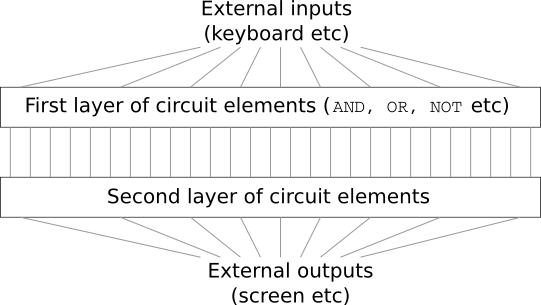
\includegraphics[width=0.833\textwidth]{images/shallow_circuit.png}
\end{center}

\noindent 你目瞪口呆，对老板说：``客户疯了！''

你的老板回答：``我也觉得他们疯了. 但客户想要什么，就得给他们什么.''

事实上，在有限的意义上，客户并没有疯. 假设你可以使用一种特殊的逻辑门，它允许你把任意多个输入 \texttt{AND} 在一起. 而且你还可以使用一个多输入 \texttt{NAND} 门，也就是说，一个可以将多个输入 \texttt{AND} 起来然后对输出取反的门. 有了这些特殊的门，事实证明可以用一个仅两层的电路来计算任意函数.

但仅仅因为某件事是可能的，并不意味着它是一个好主意. 在实践中，当解决电路设计问题（或几乎任何类型的算法问题）时，我们通常先弄清楚如何解决子问题，然后逐步整合这些解决方案. 换句话说，我们通过多层抽象来构建解决方案.

例如，假设我们正在设计一个逻辑电路来将两个数相乘. 很可能我们希望用执行两个数相加等操作的子电路来构建它. 用于两个数相加的子电路，又会由用于两个比特相加的子子电路构建而成. 粗略地说，我们的电路看起来像这样：

\begin{center}
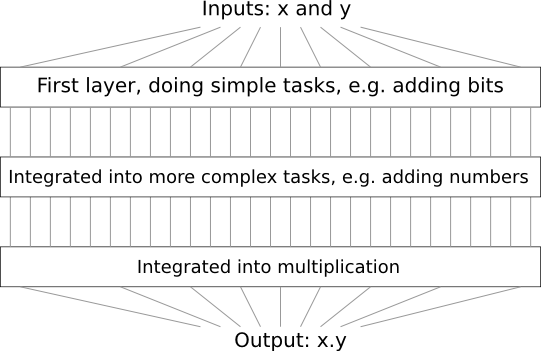
\includegraphics[width=0.833\textwidth]{images/circuit_multiplication.png}
\end{center}

\noindent 也就是说，我们最终的电路至少包含三层电路元件. 事实上，它很可能包含超过三层，因为我们会把子任务分解成比我描述的更小的单元. 但你明白大意了.

所以深层电路使设计过程更容易. 但它们不仅仅对设计有帮助. 事实上，有数学证明表明，对于某些函数，非常浅的电路需要指数级更多的电路元件才能计算，而深层电路则不需要. 例如，20 世纪 80 年代初一系列著名的论文*\footnote{这段历史有些复杂，所以我不会给出详细的参考文献. 参见 Johan Håstad 2012 年的论文 On the correlation of parity and small-depth circuits，其中有早期历史的叙述和参考文献.}表明，如果用浅层电路来计算一组比特的奇偶性，需要指数级多的门. 另一方面，如果你使用更深的电路，用一个小电路就可以轻松计算奇偶性：你只需计算每对比特的奇偶性，然后用这些结果计算每对比特对的奇偶性，依此类推，很快就能构建出整体的奇偶性. 因此，深层电路本质上可以比浅层电路强大得多.

到目前为止，本书对待神经网络的方式就像那个疯狂的客户一样. 我们使用过的几乎所有网络都只有一个隐藏神经元层（加上输入层和输出层）：

\begin{center}
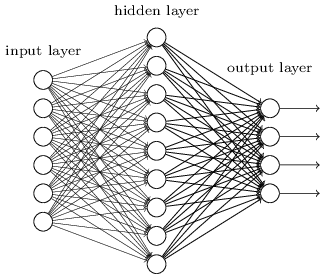
\includegraphics[width=0.9\textwidth]{images/tikz35.png}
\end{center}

\noindent 这些简单的网络非常有用：在前面的章节中，我们用这样的网络对手写数字进行分类，准确率超过了 98\%！尽管如此，直觉上我们会期望具有更多隐藏层的网络更加强大：

\begin{center}
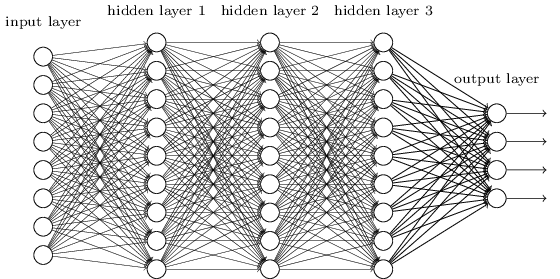
\includegraphics[width=0.9\textwidth]{images/tikz36.png}
\end{center}

\noindent 这样的网络可以利用中间层来构建多层抽象，就像我们在布尔电路中所做的那样. 例如，如果我们正在进行视觉模式识别，那么第一层的神经元可能学会识别边缘，第二层的神经元可以学会识别更复杂的形状，比如由边缘构成的三角形或矩形. 第三层则会识别更加复杂的形状. 依此类推. 这些多层抽象似乎很可能赋予深层网络在学习解决复杂模式识别问题方面的显著优势. 此外，正如电路的情况一样，有理论结果表明深层网络本质上比浅层网络更加强大*\footnote{对于某些问题和网络架构，这一点在 On the number of response regions of deep feed forward networks with piece-wise linear activations 中得到了证明，作者是 Razvan Pascanu、Guido Montúfar 和 Yoshua Bengio（2014）. 另见 Yoshua Bengio（2009）的 Learning deep architectures for AI 第 2 节中更非正式的讨论.}.

我们如何训练这样的深层网络呢？在本章中，我们将尝试使用我们的主力学习算法——通过反向传播的随机梯度下降——来训练深层网络. 但我们会遇到麻烦，我们的深层网络表现并不比浅层网络好多少（如果有的话）.

鉴于上面的讨论，这种失败似乎令人惊讶. 我们不会放弃深层网络，而是要深入挖掘，试图理解是什么让我们的深层网络难以训练. 当我们仔细观察时，我们会发现深层网络中不同的层以极其不同的速度学习. 特别是，当网络中较后的层学习得很好时，较早的层在训练过程中常常陷入停滞，几乎学不到任何东西. 这种停滞不仅仅是运气不好. 相反，我们会发现学习放缓的发生有根本性的原因，与我们使用基于梯度的学习技术有关.

当我们更深入地探究这个问题时，我们会了解到相反的现象也可能发生：较早的层可能学习得很好，但较后的层可能陷入停滞. 事实上，我们会发现，在深层的多层神经网络中，通过梯度下降进行学习存在一种内在的不稳定性. 这种不稳定性往往导致较早或较后的层在训练过程中陷入停滞.

这一切听起来像是坏消息. 但通过深入研究这些困难，我们可以开始洞察有效训练深层网络所需的条件. 因此这些研究为下一章做了很好的准备，在下一章中我们将使用深度学习来攻克图像识别问题.
\sectionTitle{梯度消失问题}{梯度消失问题}

那么，当我们尝试训练一个深度网络时，究竟出了什么问题？

为了回答这个问题，让我们首先回顾一下只有一个隐藏层的网络的情况. 像往常一样，我们将使用 MNIST 数字分类问题作为学习和实验的游乐场*\footnote{我在这里和这里介绍了 MNIST 问题和数据.}.

如果你愿意，你可以在自己的计算机上训练网络来跟随学习. 当然，仅仅阅读也是可以的. 如果你确实想实时跟随，那么你需要 Python 2.7、Numpy 以及一份代码，你可以通过从命令行克隆相关仓库来获取：

\begin{lstlisting}
git clone https://github.com/mnielsen/neural-networks-and-deep-learning.git

\end{lstlisting}

如果你不使用 git，那么你可以在这里下载数据和代码. 你需要切换到 src 子目录.

然后，从 Python shell 中加载 MNIST 数据：

\begin{lstlisting}
>>> import mnist_loader
>>> training_data, validation_data, test_data = \
... mnist_loader.load_data_wrapper()

\end{lstlisting}

我们建立网络：

\begin{lstlisting}
>>> import network2
>>> net = network2.Network([784, 30, 10])

\end{lstlisting}

这个网络在输入层有 784 个神经元，对应于输入图像中的 $28 \times 28 = 784$ 个像素. 我们使用 30 个隐藏神经元，以及 10 个输出神经元，对应于 MNIST 数字的 10 种可能分类（'0'、'1'、'2'、$\ldots$、'9'）.

让我们尝试用 30 个完整的轮次来训练我们的网络，每次使用 10 个训练样本的小批量，学习率 $\eta = 0.1$，正则化参数 $\lambda = 5.0$. 在训练过程中，我们将监控 \texttt{validation\_\allowbreak{}data} 上的分类准确率*\footnote{请注意，根据你机器的速度，网络训练可能需要几分钟. 因此，如果你正在运行代码，你可能希望继续阅读并稍后回来，而不是等待代码执行完毕.}：

\begin{lstlisting}
>>> net.SGD(training_data, 30, 10, 0.1, lmbda=5.0,
... evaluation_data=validation_data, monitor_evaluation_accuracy=True)

\end{lstlisting}

我们得到了 96.48\% 的分类准确率（或大致如此——每次运行会略有不同），与我们之前使用类似配置得到的结果相当.

现在，让我们再添加一个隐藏层，同样包含 30 个神经元，并尝试使用相同的超参数进行训练：

\begin{lstlisting}
>>> net = network2.Network([784, 30, 30, 10])
>>> net.SGD(training_data, 30, 10, 0.1, lmbda=5.0,
... evaluation_data=validation_data, monitor_evaluation_accuracy=True)

\end{lstlisting}

这给出了一个改进的分类准确率，96.90\%. 这令人鼓舞：稍微增加一点深度是有帮助的. 让我们再添加一个 30 个神经元的隐藏层：

\begin{lstlisting}
>>> net = network2.Network([784, 30, 30, 30, 10])
>>> net.SGD(training_data, 30, 10, 0.1, lmbda=5.0,
... evaluation_data=validation_data, monitor_evaluation_accuracy=True)

\end{lstlisting}

这完全没有帮助. 事实上，结果回落到了 96.57\%，接近我们最初的浅层网络. 假设我们再插入一个隐藏层：

\begin{lstlisting}
>>> net = network2.Network([784, 30, 30, 30, 30, 10])
>>> net.SGD(training_data, 30, 10, 0.1, lmbda=5.0,
... evaluation_data=validation_data, monitor_evaluation_accuracy=True)

\end{lstlisting}

分类准确率再次下降，降至 96.53\%. 这可能不是一个统计上显著的下降，但也不令人鼓舞.

这种行为似乎很奇怪. 直观上，额外的隐藏层应该使网络能够学习更复杂的分类函数，从而更好地进行分类. 当然，情况不应该变得更糟，因为额外的层在最坏的情况下可以简单地什么都不做*\footnote{参见后面的这个习题，了解如何构建一个什么都不做的隐藏层.}. 但事实并非如此.

那么到底发生了什么？让我们假设额外的隐藏层原则上确实可能有帮助，问题在于我们的学习算法没有找到正确的权重和偏置. 我们想弄清楚我们的学习算法出了什么问题，以及如何做得更好.

为了对问题所在有所了解，让我们可视化网络是如何学习的. 下面，我绘制了一个 $[784, 30, 30, 10]$ 网络的一部分，即一个有两个隐藏层的网络，每个隐藏层包含 $30$ 个隐藏神经元. 图中的每个神经元上都有一个小条，表示该神经元在网络学习过程中变化的速度. 大条意味着该神经元的权重和偏置变化很快，而小条意味着权重和偏置变化缓慢. 更精确地说，这些条表示每个神经元的梯度 $\partial C / \partial b$，即代价相对于神经元偏置的变化率. 在第 2 章中我们看到，这个梯度量不仅控制了学习过程中偏置变化的速度，也控制了输入到该神经元的权重变化的速度. 如果你不记得细节，不用担心：需要记住的只是，这些条显示了每个神经元的权重和偏置在网络学习过程中变化的速度.

为了保持图简单，我只展示了两个隐藏层中前六个神经元. 我省略了输入神经元，因为它们没有需要学习的权重或偏置. 我也省略了输出神经元，因为我们正在进行逐层比较，而比较具有相同神经元数量的层最有意义. 结果绘制在训练的最开始，即网络初始化之后立即. 它们在这里*\footnote{绘制的数据是使用程序 generate\_\allowbreak{}gradient.py 生成的. 同一程序也用于生成本节后面引用的结果.}：网络是随机初始化的，因此神经元学习速度存在很大差异并不奇怪. 尽管如此，引人注目的是第二个隐藏层中的条大多比第一个隐藏层中的条大得多. 因此，第二个隐藏层中的神经元将比第一个隐藏层中的神经元学习得快得多. 这仅仅是巧合，还是第二个隐藏层中的神经元通常可能比第一个隐藏层中的神经元学习得更快？

为了确定是否如此，有一种全局的方法来比较第一和第二隐藏层的学习速度会很有帮助. 为此，让我们将梯度记为 $\delta^l_j = \partial C / \partial b^l_j$，即第 $l$ 层中第 $j$ 个神经元的梯度*\footnote{在第 2 章中我们将其称为误差，但这里我们将采用非正式的术语``梯度''. 我说``非正式''是因为这当然没有明确包括代价相对于权重的偏导数 $\partial C / \partial w$.}. 我们可以将梯度 $\delta^1$ 视为一个向量，其元素决定了第一个隐藏层学习的速度，而 $\delta^2$ 视为一个向量，其元素决定了第二个隐藏层学习的速度. 然后我们将使用这些向量的长度作为各层学习速度的（粗略的！）全局度量. 例如，长度 $\| \delta^1 \|$ 衡量第一个隐藏层学习的速度，而长度 $\| \delta^2 \|$ 衡量第二个隐藏层学习的速度.

有了这些定义，在与上面绘制的相同配置中，我们发现 $\| \delta^1 \| = 0.07\ldots$ 和 $\| \delta^2 \| = 0.31\ldots$. 因此这证实了我们之前的怀疑：第二个隐藏层中的神经元确实比第一个隐藏层中的神经元学习得快得多.

如果我们添加更多的隐藏层会发生什么？如果我们有三个隐藏层，在一个 $[784, 30, 30, 30, 10]$ 网络中，那么各自的学习速度结果是 0.012、0.060 和 0.283. 同样，较早的隐藏层比较晚的隐藏层学习得慢得多. 假设我们再添加一个包含 $30$ 个隐藏神经元的层. 在这种情况下，各自的学习速度是 0.003、0.017、0.070 和 0.285. 模式保持不变：较早的层比较晚的层学习得慢.

我们一直在观察训练开始时的学习速度，即网络初始化之后立即. 随着我们训练网络，学习速度如何变化？让我们回到只有两个隐藏层的网络. 学习速度变化如下：

\begin{center}
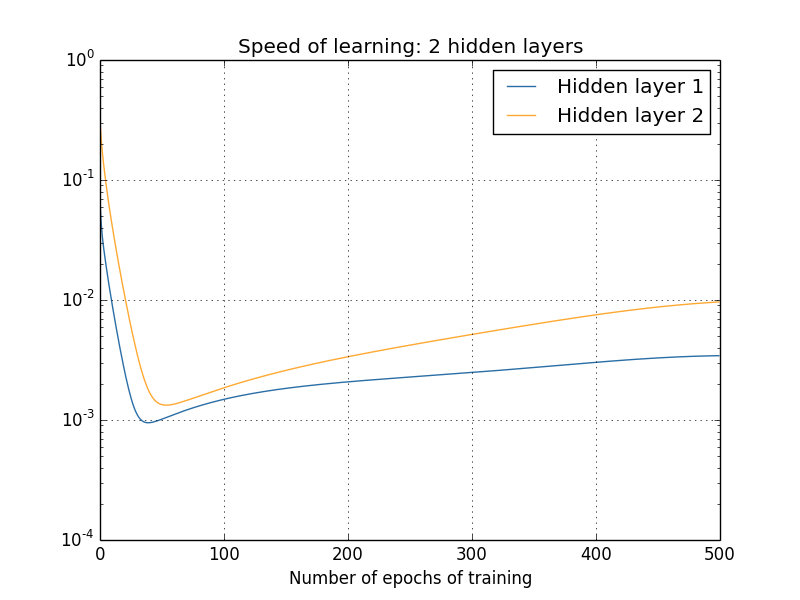
\includegraphics[width=0.833\textwidth]{images/training_speed_2_layers.png}
\end{center}

\noindent 为了生成这些结果，我使用了批量梯度下降，仅用 1,000 张训练图像，训练了 500 个轮次. 这与我们通常的训练方式有些不同——我没有使用小批量，只用了 1,000 张训练图像，而不是完整的 50,000 张图像训练集. 我不是想做什么偷偷摸摸的事，或者蒙蔽你的眼睛，但事实证明，使用小批量随机梯度下降会得到噪声大得多的结果（尽管当你平均掉噪声后，结果非常相似）. 使用我选择的参数是一种平滑结果的简单方法，这样我们就可以看到发生了什么.

无论如何，如你所见，两层一开始的学习速度非常不同（正如我们已经知道的）. 两层的速度随后都迅速下降，然后反弹. 但贯穿始终，第一个隐藏层比第二个隐藏层学习得慢得多.

更复杂的网络呢？这里是一个类似实验的结果，但这次有三个隐藏层（一个 $[784, 30, 30, 30, 10]$ 网络）：

\begin{center}
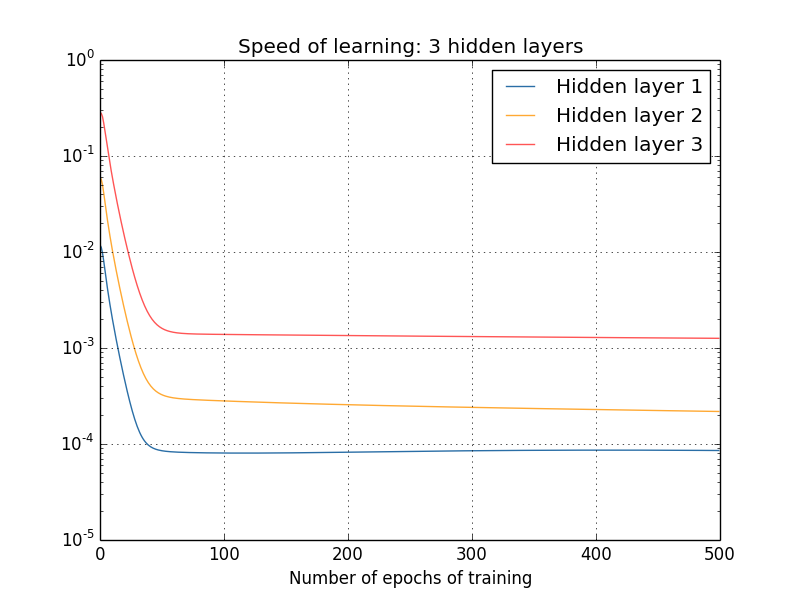
\includegraphics[width=0.833\textwidth]{images/training_speed_3_layers.png}
\end{center}

\noindent 同样，较早的隐藏层比较晚的隐藏层学习得慢得多. 最后，让我们添加第四个隐藏层（一个 $[784, 30, 30, 30, 30, 10]$ 网络），看看训练时会发生什么：

\begin{center}
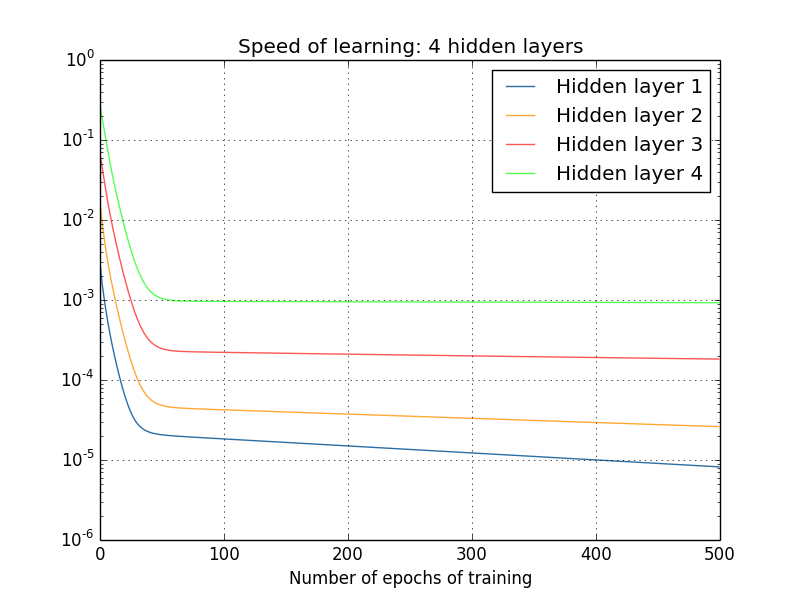
\includegraphics[width=0.833\textwidth]{images/training_speed_4_layers.png}
\end{center}

\noindent 同样，较早的隐藏层比较晚的隐藏层学习得慢得多. 在这种情况下，第一个隐藏层的学习速度大约比最后一个隐藏层慢 100 倍. 难怪我们之前训练这些网络时遇到了麻烦！

我们在这里有一个重要的观察：至少在一些深度神经网络中，梯度随着我们向后穿过隐藏层而趋于变小. 这意味着较早层中的神经元比较晚层中的神经元学习得慢得多. 虽然我们只是在一个网络中看到了这一点，但在许多神经网络中，这种情况的发生有根本原因. 这种现象被称为\emph{梯度消失问题}（vanishing gradient problem）\label{term:63}*\footnote{参见 Gradient flow in recurrent nets: the difficulty of learning long-term dependencies，作者 Sepp Hochreiter、Yoshua Bengio、Paolo Frasconi 和 Jürgen Schmidhuber（2001）. 这篇论文研究的是循环神经网络，但基本现象与我们正在研究的前馈网络相同. 另见 Sepp Hochreiter 早期的文凭论文，Untersuchungen zu dynamischen neuronalen Netzen（1991，德文）.}.

为什么会发生梯度消失问题？有没有办法避免它？在训练深度神经网络时，我们应该如何处理它？事实上，我们很快就会了解到，这并非不可避免，尽管替代方案也不太吸引人：有时梯度在较早的层中变得大得多！这就是\emph{梯度爆炸问题}（exploding gradient problem）\label{term:64}，它并不比梯度消失问题好多少. 更一般地说，事实证明深度神经网络中的梯度是\emph{不稳定的}，在较早的层中倾向于要么爆炸要么消失. 这种不稳定性是深度神经网络中基于梯度的学习的一个根本问题. 这是我们需要理解的，如果可能的话，需要采取措施解决的问题.

对梯度消失（或不稳定）的一种回应是怀疑它们是否真的是一个大问题. 暂时离开神经网络，想象我们试图数值最小化一个单变量函数 $f(x)$. 如果导数 $f'(x)$ 很小，难道不是好消息吗？难道不意味着我们已经接近极值点了吗？类似地，深度网络早期层中的小梯度是否可能意味着我们不需要对权重和偏置做太多调整？

当然，事实并非如此. 回想一下，我们随机初始化了网络中的权重和偏置. 我们初始的权重和偏置极不可能在我们希望网络做的任何事情上表现良好. 具体来说，考虑一个用于 MNIST 问题的 $[784, 30, 30, 30, 10]$ 网络中的第一层权重. 随机初始化意味着第一层丢弃了关于输入图像的大部分信息. 即使后面的层已经经过了广泛的训练，它们仍然会发现识别输入图像极其困难，仅仅因为它们没有足够的信息. 因此，第一层不需要做太多学习的情况不可能成立. 如果我们要训练深度网络，我们需要弄清楚如何解决梯度消失问题.
\sectionTitle{是什么导致了梯度消失问题？深度神经网络中不稳定的梯度}{是什么导致了梯度消失问题？深度神经网络中不稳定的梯度}

为了深入理解梯度消失问题为何会发生，让我们考虑最简单的深度神经网络：每一层只有一个神经元. 下面是一个有三个隐藏层的网络：

\begin{center}
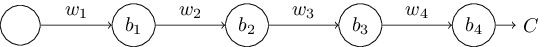
\includegraphics[width=0.9\textwidth]{images/tikz37.png}
\end{center}

\noindent 这里，$w_1, w_2, \ldots$ 是权重，$b_1, b_2, \ldots$ 是偏置，$C$ 是某个代价函数. 为了提醒你它的工作原理，第 $j$ 个神经元的输出 $a_j$ 是 $\sigma(z_j)$，其中 $\sigma$ 是通常的 S 型激活函数，而 $z_j = w_{j} a_{j-1}+b_j$ 是该神经元的加权输入. 我在最后画出了代价 $C$，以强调代价是网络输出 $a_4$ 的函数：如果网络的实际输出接近期望输出，那么代价就低，而如果相差很远，代价就高.

我们将研究第一个隐藏神经元对应的梯度 $\partial C / \partial b_1$. 我们会推导出 $\partial C / \partial b_1$ 的表达式，并通过研究该表达式来理解梯度消失问题为何会发生.

我先直接给你展示 $\partial C / \partial b_1$ 的表达式. 它看起来令人生畏，但实际上有一个简单的结构，我稍后会描述. 下面是这个表达式（暂时忽略网络，注意 $\sigma'$ 只是 $\sigma$ 函数的导数）：

\begin{center}
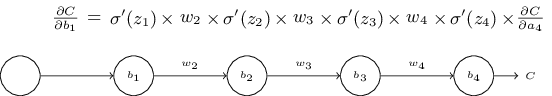
\includegraphics[width=0.9\textwidth]{images/tikz38.png}
\end{center}

\noindent 该表达式的结构如下：网络中每个神经元对应一个 $\sigma'(z_j)$ 项；网络中每个权重对应一个权重 $w_j$ 项；最后还有一个 $\partial C / \partial a_4$ 项，对应于末端的代价函数. 注意我把每一项都放在了网络中对应部分的上方. 因此，网络本身就是该表达式的一个助记符.

你可以直接接受这个表达式，跳到关于它与梯度消失问题关系的讨论. 这样做没有坏处，因为该表达式是我们之前讨论的反向传播的一个特例. 但关于这个表达式为何成立也有一个简单的解释，所以看一看那个解释是很有趣的（也许还有启发意义）.

想象我们对偏置 $b_1$ 做一个微小的改变 $\Delta b_1$. 这会在网络的其余部分引发一连串的变化. 首先，它导致第一个隐藏神经元的输出发生改变 $\Delta a_1$. 这反过来又会导致第二个隐藏神经元的加权输入发生改变 $\Delta z_2$. 然后第二个隐藏神经元的输出发生改变 $\Delta a_2$. 以此类推，一直到输出端的代价发生改变 $\Delta C$. 我们有

\begin{equation}
\frac{\partial C}{\partial b_1} \approx \frac{\Delta C}{\Delta b_1}.
\tag{114}
\end{equation}

\noindent 这表明我们可以通过仔细追踪这一连串变化中每一步的影响，来推导出梯度 $\partial C / \partial b_1$ 的表达式.

为此，让我们思考 $\Delta b_1$ 如何导致第一个隐藏神经元的输出 $a_1$ 发生变化. 我们有 $a_1 = \sigma(z_1) = \sigma(w_1 a_0 + b_1)$，所以

\begin{align}
\Delta a_1 &\approx \frac{\partial \sigma(w_1 a_0+b_1)}{\partial b_1} \Delta b_1 \tag{115} \\ &= \sigma'(z_1) \Delta b_1. \tag{116}
\end{align}

\noindent 那个 $\sigma'(z_1)$ 项应该看起来很熟悉：它是我们所声称的梯度 $\partial C / \partial b_1$ 表达式中的第一项. 直观地说，这一项将偏置的变化 $\Delta b_1$ 转换为输出激活值的变化 $\Delta a_1$. 这个变化 $\Delta a_1$ 反过来又导致第二个隐藏神经元的加权输入 $z_2 = w_2 a_1 + b_2$ 发生变化：

\begin{align}
\Delta z_2 &\approx \frac{\partial z_2}{\partial a_1} \Delta a_1 \tag{117} \\ &= w_2 \Delta a_1. \tag{118}
\end{align}

\noindent 将 $\Delta z_2$ 和 $\Delta a_1$ 的表达式结合起来，我们看到了偏置 $b_1$ 的变化如何沿着网络传播以影响 $z_2$：

\begin{equation}
\Delta z_2 \approx \sigma'(z_1) w_2 \Delta b_1.
\tag{119}
\end{equation}

\noindent 同样，这应该看起来很熟悉：我们现在得到了我们所声称的梯度 $\partial C / \partial b_1$ 表达式中的前两项.

我们可以继续以这种方式追踪变化在网络其余部分传播的方式. 在每个神经元处我们得到一个 $\sigma'(z_j)$ 项，每经过一个权重我们得到一个 $w_j$ 项. 最终结果是代价的最终变化 $\Delta C$ 与偏置的初始变化 $\Delta b_1$ 之间的关系式：

\begin{equation}
\Delta C \approx \sigma'(z_1) w_2 \sigma'(z_2) \ldots \sigma'(z_4) \frac{\partial C}{\partial a_4} \Delta b_1.
\tag{120}
\end{equation}

\noindent 除以 $\Delta b_1$，我们确实得到了所期望的梯度表达式：

\begin{equation}
\frac{\partial C}{\partial b_1} = \sigma'(z_1) w_2 \sigma'(z_2) \ldots \sigma'(z_4) \frac{\partial C}{\partial a_4}.
\tag{121}
\end{equation}

\noindent \textbf{梯度消失问题为何会发生：} 为了理解梯度消失问题为何会发生，让我们明确写出梯度的完整表达式：

\begin{equation}
\frac{\partial C}{\partial b_1} = \sigma'(z_1) \, w_2 \sigma'(z_2) \, w_3 \sigma'(z_3) \, w_4 \sigma'(z_4) \, \frac{\partial C}{\partial a_4}.
\tag{122}
\end{equation}

\noindent 除了最后一项之外，这个表达式是形如 $w_j \sigma'(z_j)$ 的项的乘积. 为了理解这些项各自的行为，让我们看一下函数 $\sigma'$ 的图像：导数在 $\sigma'(0) = 1/4$ 处达到最大值. 现在，如果我们使用标准的权重初始化方法，那么我们会用均值为 $0$、标准差为 $1$ 的高斯分布来选择权重. 所以权重通常会满足 $|w_j| < 1$. 把这些观察放在一起，我们看到项 $w_j \sigma'(z_j)$ 通常会满足 $|w_j \sigma'(z_j)| < 1/4$. 而当我们取许多这样项的乘积时，乘积会倾向于指数级减小：项越多，乘积就越小. 这开始像是梯度消失问题的一个可能解释了.

为了把这一切说得更明确一些，让我们把 $\partial C / \partial b_1$ 的表达式与关于后面某个偏置的梯度表达式进行比较，比如 $\partial C / \partial b_3$. 当然，我们还没有明确推导出 $\partial C / \partial b_3$ 的表达式，但它遵循上面描述的与 $\partial C / \partial b_1$ 相同的模式. 下面是两个表达式的比较：

\begin{center}
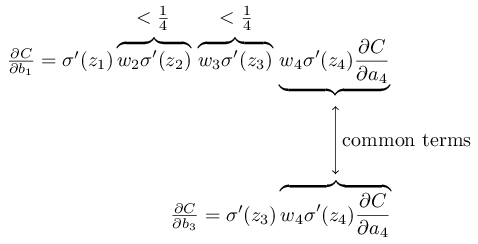
\includegraphics[width=0.9\textwidth]{images/tikz39.png}
\end{center}

\noindent 这两个表达式共享许多项. 但梯度 $\partial C / \partial b_1$ 多包含了两个形如 $w_j \sigma'(z_j)$ 的项. 正如我们所看到的，这样的项通常大小小于 $1/4$. 因此梯度 $\partial C / \partial b_1$ 通常会比 $\partial C / \partial b_3$ 小 $16$ 倍（或更多）. 这就是梯度消失问题的本质根源.

当然，这是一个非正式的论证，而不是梯度消失问题一定会发生的严格证明. 存在几种可能的例外情况. 特别地，我们可能会想权重 $w_j$ 在训练过程中是否会增大. 如果它们增大了，那么乘积中的项 $w_j \sigma'(z_j)$ 可能不再满足 $|w_j \sigma'(z_j)| < 1/4$. 确实，如果这些项变得足够大——大于 $1$——那么我们将不再有梯度消失问题. 相反，当我们反向穿过各层时，梯度实际上会指数级增长. 我们将遇到的不是梯度消失问题，而是梯度爆炸\label{term:66}问题.\textbf{梯度爆炸问题：} 让我们看一个梯度爆炸发生的具体例子. 这个例子有些人为构造：我将以恰到好处的方式固定网络中的参数，以确保我们得到梯度爆炸. 但即使这个例子是人为构造的，它的优点在于牢固地确立了梯度爆炸不仅仅是一种假设的可能性，它们确实可以发生.

得到梯度爆炸需要两个步骤. 首先，我们选择网络中所有较大的权重，比如 $w_1 = w_2 = w_3 = w_4 = 100$. 其次，我们选择偏置使得 $\sigma'(z_j)$ 项不会太小. 这实际上很容易做到：我们只需要选择偏置使得每个神经元的加权输入为 $z_j = 0$（从而 $\sigma'(z_j) = 1/4$）. 例如，我们想要 $z_1 = w_1 a_0 + b_1 = 0$. 我们可以通过设置 $b_1 = -100 * a_0$ 来实现这一点. 我们可以用同样的思路来选择其他偏置. 当我们这样做时，我们看到所有项 $w_j \sigma'(z_j)$ 都等于 $100 * \frac{1}{4} = 25$. 有了这些选择，我们就得到了梯度爆炸.\textbf{不稳定的梯度问题：} 这里根本的问题与其说是梯度消失问题或梯度爆炸问题，不如说是早期层中的梯度是所有后面层中项的乘积. 当有很多层时，这本质上是一种不稳定的情况. 所有层能够以接近相同的速度学习的唯一方式是所有这些项的乘积接近相互平衡. 如果没有某种机制或内在原因使得这种平衡发生，它极不可能仅仅靠偶然发生. 简而言之，这里真正的问题是神经网络遭受\emph{不稳定的梯度问题}（unstable gradient problem）\label{term:65}. 因此，如果我们使用标准的基于梯度的学习技术，网络中不同的层将倾向于以极其不同的速度学习.

\begin{exerciseBox}{练习}

\begin{itemize}

\item 在我们对梯度消失问题的讨论中，我们利用了 $|\sigma'(z)| < 1/4$ 这一事实. 假设我们使用一个不同的激活函数，其导数可能大得多. 这能帮助我们避免不稳定的梯度\label{term:67}问题吗？

\end{itemize}

\textbf{梯度消失问题的普遍性：} 我们已经看到，在深度网络的早期层中梯度要么消失要么爆炸. 事实上，当使用 S 型神经元时，梯度通常会消失. 要理解原因，再次考虑表达式 $|w \sigma'(z)|$. 为了避免梯度消失问题，我们需要 $|w \sigma'(z)| \geq 1$. 你可能认为如果 $w$ 非常大，这很容易发生. 然而，这比看起来要困难. 原因是 $\sigma'(z)$ 项也依赖于 $w$：$\sigma'(z) = \sigma'(wa +b)$，其中 $a$ 是输入激活值. 所以当我们使 $w$ 变大时，我们需要注意不要同时使 $\sigma'(wa+b)$ 变小. 事实证明这是一个相当大的约束. 原因是当我们使 $w$ 变大时，我们倾向于使 $wa+b$ 非常大. 看着 $\sigma'$ 的图像，你可以看到这把我们带到了 $\sigma'$ 函数的``两翼''，在那里它取非常小的值. 避免这种情况的唯一方法是输入激活值落在一个相当窄的值范围内（这个定性解释在下面的第一个习题中被定量化）. 有时这会碰巧发生. 但更常见的是，它不会发生. 所以在一般情况下我们有梯度消失.

\end{exerciseBox}

\begin{exerciseBox}{习题}

\begin{itemize}

\item
考虑乘积 $|w \sigma'(wa+b)|$. 假设 $|w \sigma'(wa+b)| \geq 1$.(1) 论证这只有在 $|w| \geq 4$ 时才可能发生.(2) 假设 $|w| \geq 4$，考虑满足 $|w \sigma'(wa+b)| \geq 1$ 的输入激活值 $a$ 的集合. 证明满足该约束的 $a$ 的集合所覆盖的区间宽度不超过

\begin{equation}
\frac{2}{|w|} \ln\left( \frac{|w|(1+\sqrt{1-4/|w|})}{2}-1\right).
\tag{123}
\end{equation}

(3) 用数值方法证明上述界定区间宽度的表达式在 $|w| \approx 6.9$ 处最大，此时它取值 $\approx 0.45$. 因此，即使一切都完美地对齐，我们仍然只有一个相当窄的输入激活值范围可以避免梯度消失问题.

\item \textbf{恒等神经元：} 考虑一个神经元，它有一个输入 $x$，对应的权重 $w_1$，一个偏置 $b$，以及输出上的权重 $w_2$. 证明通过适当地选择权重和偏置，我们可以确保对于 $x \in [0, 1]$ 有 $w_2 \sigma(w_1 x+b) \approx x$. 这样的神经元因此可以被用作一种恒等神经元，即一个输出与其输入相同（至多相差一个权重因子的缩放）的神经元.\emph{提示：把 $x = 1/2+\Delta$ 重写，假设 $w_1$ 很小，并对 $w_1 \Delta$ 使用泰勒级数展开，这些都会有所帮助.}

\end{itemize}

\end{exerciseBox}
\sectionTitle{更复杂网络中不稳定的梯度}{更复杂网络中不稳定的梯度}

我们一直在研究玩具网络，每个隐藏层只有一个神经元. 那么更复杂的深度网络呢，每个隐藏层中有许多神经元？

\begin{center}
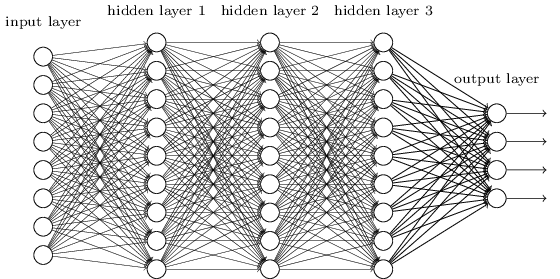
\includegraphics[width=0.9\textwidth]{images/tikz40.png}
\end{center}

事实上，这类网络中会出现大致相同的行为. 在之前关于反向传播的章节中，我们看到 $L$ 层网络中第 $l$ 层的梯度由下式给出：

\begin{equation}
\delta^l = \Sigma'(z^l) (w^{l+1})^T \Sigma'(z^{l+1}) (w^{l+2})^T \ldots \Sigma'(z^L) \nabla_a C
\tag{124}
\end{equation}

\noindent 这里，$\Sigma'(z^l)$ 是一个对角矩阵，其对角线元素是第 $l$ 层加权输入的 $\sigma'(z)$ 值. $w^l$ 是不同层的权重矩阵. 而 $\nabla_a C$ 是 $C$ 关于输出激活值的偏导数向量.

这比单神经元情形下的表达式要复杂得多. 不过，如果你仔细观察，其基本形式非常相似，包含许多形如 $(w^j)^T \Sigma'(z^j)$ 的项对. 更重要的是，矩阵 $\Sigma'(z^j)$ 的对角线元素很小，没有一个大于 $\frac{1}{4}$. 只要权重矩阵 $w^j$ 不太大，每个额外的项 $(w^j)^T \Sigma'(z^l)$ 都会倾向于使梯度向量变小，从而导致梯度消失. 更一般地，乘积中大量的项倾向于导致不稳定的梯度，正如我们之前的例子那样. 在实践中，经验上通常发现，在 S 型网络中，梯度在较早的层中会以指数速度迅速消失. 结果，这些层中的学习会减慢. 这种减慢不仅仅是偶然的或不方便的事情：它是我们采用的学习方法的根本后果.
\sectionTitle{深度学习的其他障碍}{深度学习的其他障碍}

在本章中，我们关注了梯度消失——更一般地说，不稳定的梯度——作为深度学习的一个障碍. 事实上，不稳定的梯度只是深度学习的一个障碍，尽管它是一个重要的根本性障碍. 许多正在进行的研究旨在更好地理解训练深度网络时可能出现的挑战. 我不会在这里全面总结这些工作，而只是想简要提及几篇论文，让你感受一下人们正在提出的一些问题.

作为第一个例子，2010 年 Glorot 和 Bengio*\footnote{Understanding the difficulty of training deep feedforward neural networks, by Xavier Glorot and Yoshua Bengio (2010). See also the earlier discussion of the use of sigmoids in Efficient BackProp, by Yann LeCun, Léon Bottou, Genevieve Orr and Klaus-Robert Müller (1998).} 发现了证据，表明使用 S 型激活函数可能会导致训练深度网络时出现问题. 特别地，他们发现证据表明，使用 S 型函数会导致最终隐藏层中的激活值在训练早期就饱和在 $0$ 附近，从而大幅减慢学习速度. 他们提出了一些替代的激活函数，这些函数似乎不太受这个饱和问题的影响.

作为第二个例子，2013 年 Sutskever、Martens、Dahl 和 Hinton*\footnote{On the importance of initialization and momentum in deep learning, by Ilya Sutskever, James Martens, George Dahl and Geoffrey Hinton (2013).} 研究了随机权重初始化和基于动量的随机梯度下降中的动量日程对深度学习的影响. 在这两种情况下，做出好的选择对训练深度网络的能力产生了实质性的差异.

这些例子表明，``是什么让深度网络难以训练？'' 是一个复杂的问题. 在本章中，我们关注了与深度网络中基于梯度的学习相关的不稳定性. 最后两段中的结果表明，激活函数的选择、权重的初始化方式，甚至梯度下降学习的实现细节也发挥着作用. 当然，网络结构和其他超参数的选择也很重要. 因此，许多因素都可能在使深度网络难以训练中发挥作用，而理解所有这些因素仍然是一个正在进行的研究课题. 这一切似乎相当令人沮丧和悲观. 但好消息是，在下一章中我们将扭转局面，并开发几种深度学习方法，这些方法在一定程度上设法克服或绕开所有这些挑战.

\chapter{深度学习}
在上一章中我们了解到，深度神经网络通常比浅层神经网络更难训练. 这很不幸，因为我们有充分的理由相信，\emph{如果}我们能训练深度网络，它们会比浅层网络强大得多. 但是，尽管上一章传来的消息令人沮丧，我们不会让它阻止我们. 在本章中，我们将开发可用于训练深度网络的技术，并将它们付诸实践. 我们还将审视更广阔的图景，简要回顾使用深度网络进行图像识别、语音识别和其他应用的最新进展. 并且我们将简要而带有推测性地展望神经网络和人工智能的未来.

本章篇幅较长. 为了帮助你导航，让我们先浏览一下. 各节之间耦合较松，因此只要你对神经网络有一些基本的了解，就可以跳到你最感兴趣的部分.

本章的主要部分是对最广泛使用的深度网络类型之一的介绍：深度卷积网络. 我们将通过一个详细的例子——包括代码在内的全部内容——来展示如何使用卷积网络解决从 MNIST 数据集中分类手写数字的问题：

\begin{center}

\includegraphics[width=0.267\textwidth]{images/digits.png}
\end{center}

\noindent 我们将从本书前面用于攻克这个问题的浅层网络开始讲述卷积网络. 通过多次迭代，我们将构建出越来越强大的网络. 在此过程中，我们将探索许多强大的技术：卷积、池化、使用 GPU 进行比浅层网络多得多的训练、训练数据的算法扩展（以减少过拟合）、dropout 技术的使用（同样是为了减少过拟合）、网络集成（ensemble）的使用，等等. 结果将是一个性能接近人类的系统. 在 10,000 张 MNIST 测试图像中——这些图像在训练期间从未见过！——我们的系统将正确分类 9,967 张. 下面是那 33 张被错误分类的图像的预览. 注意正确的分类在右上角；我们程序的分类在右下角：

\begin{center}
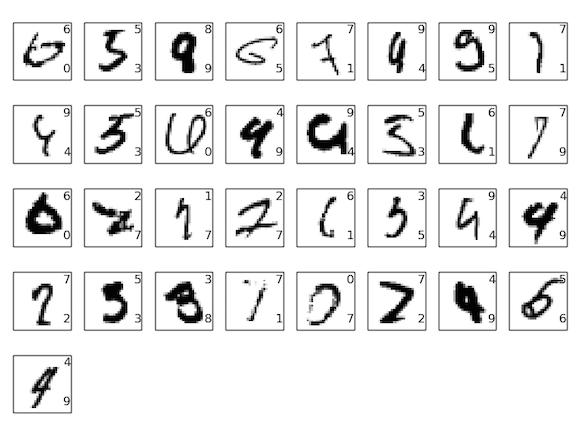
\includegraphics[width=0.967\textwidth]{images/ensemble_errors.png}
\end{center}

\noindent 其中许多图像即使对人类来说也很难分类. 例如，考虑第一行中的第三张图像. 在我看来它更像是一个 ``9'' 而不是官方分类的 ``8''. 我们的网络也认为它是一个 ``9''. 这种 ``错误'' 至少是可以理解的，甚至可能是值得称赞的. 我们以对使用网络（特别是卷积网络）进行图像识别的一些引人注目的最新进展的综述来结束关于图像识别的讨论.

本章的剩余部分从更广阔、更粗略的角度讨论深度学习. 我们将简要概述其他神经网络模型，例如循环神经网络和长短期记忆网络\label{term:68}，以及这些模型如何应用于语音识别、自然语言处理和其他领域的问题. 我们还将推测神经网络和深度学习的未来，从意图驱动的用户界面等想法，到深度学习在人工智能中的作用.

本章建立在本书前面章节的基础上，利用并整合了反向传播、正则化、softmax 函数等思想. 然而，要阅读本章，你不需要详细地学习过所有前面的章节. 不过，阅读第 1 章关于神经网络基础的内容会有所帮助. 当我使用第 2 章到第 5 章的概念时，我会提供链接，以便你在必要时熟悉它们.

值得注意的是本章不是什么. 它不是关于最新最伟大的神经网络库的教程. 我们也不会训练具有数十层的深度网络来解决最前沿的问题. 相反，重点是理解深度神经网络背后的一些核心原理，并将它们应用于 MNIST 问题这个简单、易于理解的背景中. 换句话说：本章不会把你直接带到前沿. 相反，本章和前面章节的目的是聚焦于基础，从而为你理解当前广泛的工作做好准备.
\sectionTitle{卷积网络入门}{卷积网络入门}

在前面的章节中，我们教会了神经网络相当出色地识别手写数字图像：

\begin{center}

\includegraphics[width=0.267\textwidth]{images/digits.png}
\end{center}

\noindent 我们使用的网络中，相邻的网络层之间是全连接的. 也就是说，网络中的每一个神经元都与相邻层中的每一个神经元相连：

\begin{center}
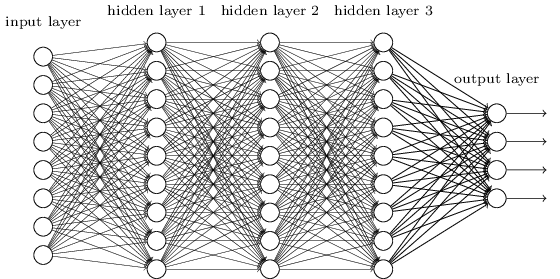
\includegraphics[width=0.9\textwidth]{images/tikz41.png}
\end{center}

\noindent 特别地，对于输入图像中的每个像素，我们将该像素的强度编码为输入层中对应神经元的值. 对于我们一直使用的 $28 \times 28$ 像素图像，这意味着我们的网络有 $784$（$= 28 \times 28$）个输入神经元. 然后我们训练网络的权重和偏置，使得网络的输出能够——我们希望如此！——正确地识别输入图像：'0'、'1'、'2'、...、'8' 或 '9'.

我们之前的网络工作得相当不错：使用 MNIST 手写数字数据集的训练和测试数据，我们获得了超过 98\% 的分类准确率. 但仔细想想，使用全连接层网络来分类图像是很奇怪的. 原因在于，这样的网络结构没有考虑图像的空间结构. 例如，它将相距很远和靠得很近的输入像素完全同等对待. 这种空间结构的概念必须从训练数据中推断出来. 但是，如果我们不是从一个\emph{白板}式的网络结构出发，而是使用一种试图利用空间结构的结构呢？在本节中，我将介绍\emph{卷积神经网络}*\footnote{卷积神经网络的起源可以追溯到 20 世纪 70 年代. 但奠定现代卷积网络这一学科的奠基性论文是 1998 年 Yann LeCun、Léon Bottou、Yoshua Bengio 和 Patrick Haffner 发表的 ``Gradient-based learning applied to document recognition''. LeCun 后来对卷积网络的术语发表了一个有趣的评论：``像卷积网络这样的模型中的[生物学]神经灵感是非常微弱的. 这就是为什么我称它们为'卷积网络'而不是'卷积神经网络'，也是为什么我们称节点为'单元'而不是'神经元' ''. 尽管有这番评论，卷积网络使用了与我们迄今为止所研究的神经网络许多相同的思想：诸如反向传播、梯度下降、正则化、非线性激活函数等等. 因此我们将遵循惯例，将它们视为一种神经网络. 我将交替使用术语``卷积神经网络''和``卷积网络''. 我也将交替使用术语``[人工]神经元''和``单元''.}. 这些网络使用一种特别适合分类图像的特殊结构. 使用这种结构使得卷积网络训练速度很快. 这反过来又帮助我们训练深层的多层网络，这些网络非常擅长分类图像. 如今，大多数用于图像识别的神经网络都使用深度卷积网络或某种接近的变体.

卷积神经网络\label{term:69}使用三个基本思想：\emph{局部感受野}、\emph{权重共享}和\emph{池化}. 让我们依次来看这些思想. \textbf{局部感受野：} 在前面展示的全连接层中，输入被描绘成一条垂直的神经元线. 在卷积网络中，将输入视为一个 $28 \times 28$ 的神经元方块会更有帮助，其值对应于我们用作输入的 $28 \times 28$ 像素强度：

\begin{center}

\includegraphics[width=0.9\textwidth]{images/tikz42.png}
\end{center}

\noindent 和往常一样，我们将输入像素连接到一层隐藏神经元. 但我们不会将每个输入像素连接到每个隐藏神经元. 相反，我们只在输入图像的小的局部区域内建立连接.

更准确地说，第一个隐藏层中的每个神经元将连接到输入神经元的一个小区域，比如说，一个 $5 \times 5$ 的区域，对应 $25$ 个输入像素. 因此，对于某个特定的隐藏神经元，我们可能有这样的连接：

\begin{center}
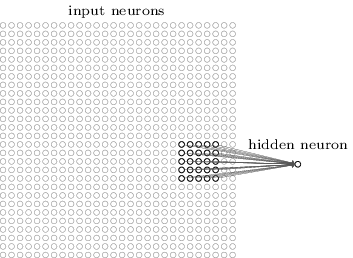
\includegraphics[width=0.9\textwidth]{images/tikz43.png}
\end{center}

\noindent 输入图像中的那个区域被称为该隐藏神经元的\emph{局部感受野}. 它是输入像素上的一个小窗口. 每个连接学习一个权重. 隐藏神经元还学习一个总的偏置. 你可以把那个特定的隐藏神经元看作是在学习分析它特定的局部感受野.

然后我们将局部感受野\label{term:70}在整个输入图像上滑动. 对于每个局部感受野，第一个隐藏层中都有一个不同的隐藏神经元. 为了具体说明这一点，让我们从左上角的一个局部感受野开始：

\begin{center}
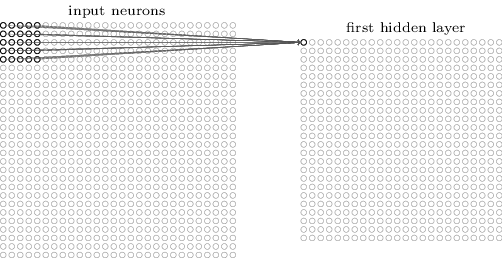
\includegraphics[width=0.9\textwidth]{images/tikz44.png}
\end{center}

\noindent 然后我们将局部感受野向右滑动一个像素（即一个神经元），连接到第二个隐藏神经元：

\begin{center}
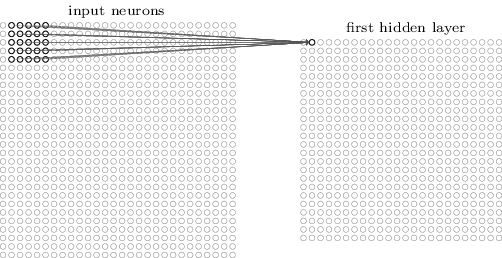
\includegraphics[width=0.9\textwidth]{images/tikz45.png}
\end{center}

\noindent 以此类推，构建出第一个隐藏层. 注意，如果我们有一个 $28 \times 28$ 的输入图像，以及 $5 \times 5$ 的局部感受野，那么隐藏层中将有 $24 \times 24$ 个神经元. 这是因为我们只能将局部感受野移动 $23$ 个神经元（或向下 $23$ 个神经元），否则就会碰到输入图像的右侧（或底部）.

我展示的是局部感受野每次移动一个像素. 事实上，有时会使用不同的\emph{步长}. 例如，我们可能将局部感受野向右（或向下）移动 $2$ 个像素，在这种情况下我们会说使用了步长 $2$. 在本章中，我们主要坚持使用步长 $1$，但值得知道的是，人们有时会尝试不同的步长*\footnote{正如前面章节所做的那样，如果我们有兴趣尝试不同的步长，那么我们可以使用验证数据来挑选出性能最佳的步长. 更多细节，请参见前面关于如何选择神经网络超参数的讨论. 同样的方法也可以用来选择局部感受野的大小——当然，使用 $5 \times 5$ 的局部感受野并没有什么特别之处. 一般来说，当输入图像明显大于 $28 \times 28$ 像素的 MNIST 图像时，更大的局部感受野往往更有帮助.}. \textbf{权重共享\label{term:71}和偏置共享：} 我说过每个隐藏神经元都有一个偏置和连接到其局部感受野的 $5 \times 5$ 个权重. 我还没有提到的是，我们将对 $24 \times 24$ 个隐藏神经元中的每一个使用\emph{相同}的权重和偏置. 换句话说，对于第 $j, k$ 个隐藏神经元，输出为：

\begin{equation}
\sigma\left(b + \sum_{l=0}^4 \sum_{m=0}^4 w_{l,m} a_{j+l, k+m} \right).
\tag{125}
\end{equation}

\noindent 这里，$\sigma$ 是神经激活函数——也许是我们在前面章节中使用的 S 型函数. $b$ 是偏置的共享值. $w_{l,m}$ 是一个 $5 \times 5$ 的共享权重数组. 最后，我们用 $a_{x, y}$ 表示位置 $x, y$ 处的输入激活值.

这意味着第一个隐藏层中的所有神经元检测完全相同的特征*\footnote{我还没有精确定义特征的概念. 非正式地说，把隐藏神经元检测到的特征看作是将导致该神经元激活的那类输入模式：例如，它可能是图像中的一条边缘，或者也许是某种其他类型的形状.}，只是在输入图像中的不同位置. 要理解为什么这是合理的，假设权重和偏置使得隐藏神经元能够挑出，比如说，某个特定局部感受野中的一条垂直边缘. 这种能力在图像的其他地方也很可能有用. 因此，在图像的每个地方应用相同的特征检测器是有用的. 用稍微更抽象的话来说，卷积网络很好地适应了图像的平移不变性：将一张猫的图片（比如说）移动一点，它仍然是一张猫的图片*\footnote{事实上，对于我们一直在研究的 MNIST 数字分类问题，图像是居中的且大小归一化的. 所以可以说，MNIST 比``在野外''发现的图像具有更少的平移不变性. 尽管如此，像边缘和角这样的特征在输入空间的大部分区域很可能是有用的.}.

出于这个原因，我们有时将输入层到隐藏层的映射称为\emph{特征图}. 我们将定义特征图的权重称为\emph{共享权重}. 我们将以这种方式定义特征图的偏置称为\emph{共享偏置}. 共享权重和偏置通常被说成定义了一个\emph{核}或\emph{滤波器}. 在文献中，人们有时以略微不同的方式使用这些术语，因此我不会更精确地定义；相反，稍后我们将看一些具体的例子.

到目前为止我描述的网络结构只能检测一种局部特征. 要进行图像识别，我们需要不止一个特征图\label{term:73}. 因此，一个完整的卷积层\label{term:72}由几个不同的特征图组成：

\begin{center}
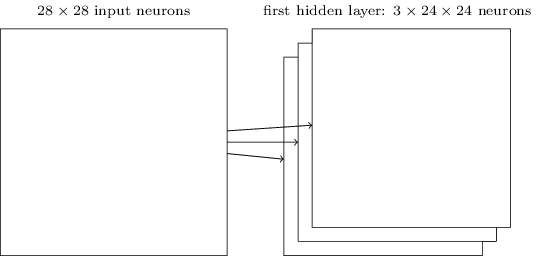
\includegraphics[width=0.9\textwidth]{images/tikz46.png}
\end{center}

\noindent 在所示的例子中，有 $3$ 个特征图. 每个特征图由一组 $5 \times 5$ 的共享权重和一个共享偏置定义. 结果是网络可以检测 $3$ 种不同的特征，每种特征都可以在整个图像中被检测到.

我只展示了 $3$ 个特征图，以使上面的图保持简单. 然而，在实践中，卷积网络可能使用更多（也许多得多）的特征图. 早期的卷积网络之一，LeNet-5，使用了 $6$ 个特征图，每个关联到一个 $5 \times 5$ 的局部感受野，来识别 MNIST 数字. 所以上面展示的例子实际上非常接近 LeNet-5. 在本章后面我们开发的例子中，我们将使用具有 $20$ 和 $40$ 个特征图的卷积层. 让我们快速看一下学习到的一些特征*\footnote{所展示的特征图来自我们训练的最终卷积网络，见这里.}：

\begin{center}
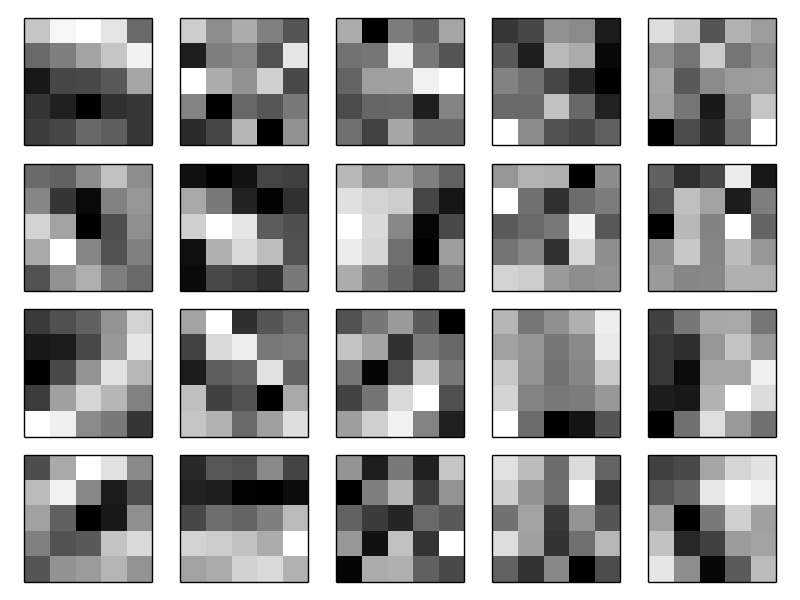
\includegraphics[width=0.667\textwidth]{images/net_full_layer_0.png}
\end{center}

\noindent 这 $20$ 张图像对应于 $20$ 个不同的特征图（或滤波器，或核）. 每个图表示为一个 $5 \times 5$ 的块图像，对应于局部感受野中的 $5 \times 5$ 个权重. 较白的块意味着较小的（通常更负的）权重，因此特征图对相应的输入像素响应较弱. 较暗的块意味着较大的权重，因此特征图对相应的输入像素响应较强. 非常粗略地说，上面的图像显示了卷积层所响应的特征类型.

那么我们能从这些特征图中得出什么结论呢？很明显，这里存在超出我们随机预期的空间结构：许多特征具有明显的亮暗子区域. 这表明我们的网络确实在学习与空间结构相关的东西. 然而，除此之外，很难看出这些特征检测器在学习什么. 当然，我们不是在学习（比如说）许多传统图像识别方法中使用的 Gabor 滤波器. 事实上，现在有大量工作致力于更好地理解卷积网络学习到的特征. 如果你有兴趣跟进这项工作，我建议从 Matthew Zeiler 和 Rob Fergus（2013）的论文 Visualizing and Understanding Convolutional Networks 开始.

共享权重和偏置的一大优势是它大大减少了卷积网络中涉及的参数数量. 对于每个特征图，我们需要 $25 = 5 \times 5$ 个共享权重，加上一个共享偏置. 所以每个特征图需要 $26$ 个参数. 如果我们有 $20$ 个特征图，那就是总共 $20 \times 26 = 520$ 个参数来定义卷积层. 相比之下，假设我们有一个全连接的第一层，有 $784 = 28 \times 28$ 个输入神经元，以及相对适中的 $30$ 个隐藏神经元，正如我们在本书前面许多例子中使用的那样. 那就是总共 $784 \times 30$ 个权重，加上额外的 $30$ 个偏置，总共 $23,550$ 个参数. 换句话说，全连接层的参数数量将是卷积层的 $40$ 倍以上.

当然，我们无法真正直接比较参数数量，因为这两个模型在本质上是不同的. 但是，直观上，卷积层利用平移不变性似乎很可能减少它达到与全连接模型相同性能所需的参数数量. 这反过来将导致卷积模型训练更快，并最终帮助我们使用卷积层构建深度网络.

顺便提一下，\emph{卷积}这个名字来源于方程 (125) 中的运算

\begin{align*}
\sigma\left(b + \sum_{l=0}^4 \sum_{m=0}^4 w_{l,m} a_{j+l, k+m} \right) \nonumber
\end{align*}
\noindent 有时被称为\emph{卷积}. 更准确地说，人们有时将该方程写为 $a^1 = \sigma(b + w * a^0)$，其中 $a^1$ 表示来自一个特征图的输出激活值集合，$a^0$ 是输入激活值集合，而 $*$ 被称为卷积运算. 我们不打算深入使用卷积的数学，所以你不需要太担心这个联系. 但至少值得知道这个名字从何而来.\textbf{池化层\label{term:74}：} 除了刚才描述的卷积层之外，卷积神经网络还包含\emph{池化层}. 池化层通常紧跟在卷积层之后使用. 池化层所做的是简化卷积层输出中的信息.

具体来说，池化层取卷积层输出的每个特征图*\footnote{这里的命名比较宽松. 特别地，我用``特征图''指的不是卷积层计算的函数，而是该层输出的隐藏神经元的激活值. 这种对命名的轻微滥用在研究文献中相当常见.}并准备一个浓缩的特征图. 例如，池化层中的每个单元可以汇总前一层中（比如）$2 \times 2$ 个神经元的区域. 作为一个具体例子，一种常见的池化过程被称为\emph{最大池化}. 在最大池化中，池化单元简单地输出 $2 \times 2$ 输入区域中的最大激活值，如下图所示：

\begin{center}
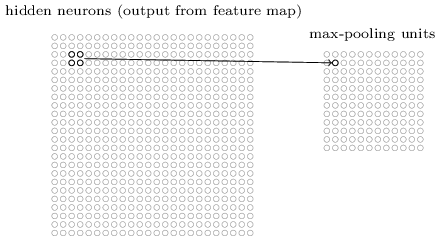
\includegraphics[width=0.9\textwidth]{images/tikz47.png}
\end{center}

\noindent 注意，由于卷积层输出 $24 \times 24$ 个神经元，池化后我们有 $12 \times 12$ 个神经元.

如上所述，卷积层通常涉及不止一个特征图. 我们对每个特征图分别应用最大池化\label{term:75}. 所以如果有三个特征图，组合的卷积层和最大池化层将如下所示：

\begin{center}
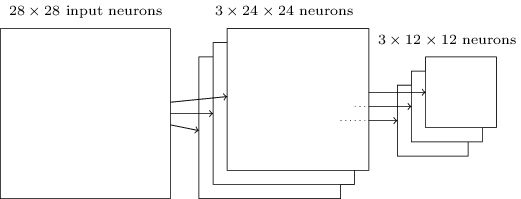
\includegraphics[width=0.9\textwidth]{images/tikz48.png}
\end{center}

\noindent 我们可以将最大池化视为网络询问给定特征是否在图像的某个区域中任何地方被找到的一种方式. 然后它丢弃精确的位置信息. 直觉是，一旦找到了一个特征，它的精确位置就不如它相对于其他特征的粗略位置那么重要. 一个很大的好处是池化后的特征少得多，因此这有助于减少后续层中所需的参数数量.

最大池化并不是用于池化的唯一技术. 另一种常见方法被称为\emph{L2 池化}. 在这里，我们不是取 $2 \times 2$ 神经元区域的最大激活值，而是取 $2 \times 2$ 区域中激活值平方和的平方根. 虽然细节不同，但直觉与最大池化相似：L2 池化是一种浓缩卷积层信息的方式. 在实践中，这两种技术都被广泛使用. 有时人们使用其他类型的池化操作. 如果你真的想优化性能，你可以使用验证数据来比较几种不同的池化方法，并选择效果最好的方法. 但我们不打算担心那种详细的优化.\textbf{整合所有内容：} 我们现在可以将所有这些想法整合在一起，形成一个完整的卷积神经网络. 它类似于我们刚才看到的架构，但增加了一层 $10$ 个输出神经元，对应于 MNIST 数字的 $10$ 个可能值（'0'、'1'、'2'、\emph{等等}）：

\begin{center}
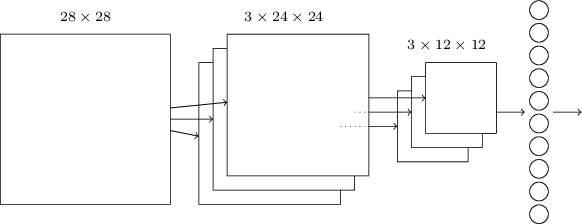
\includegraphics[width=0.9\textwidth]{images/tikz49.png}
\end{center}

\noindent 网络以 $28 \times 28$ 个输入神经元开始，用于编码 MNIST 图像的像素强度. 然后是一个使用 $5 \times 5$ 局部感受野和 $3$ 个特征图的卷积层. 结果是一层 $3 \times 24 \times 24$ 个隐藏特征神经元. 下一步是一个最大池化层，应用于 $2 \times 2$ 区域，跨越 $3$ 个特征图中的每一个. 结果是一层 $3 \times 12 \times 12$ 个隐藏特征神经元.

网络中最后一层连接是全连接层. 也就是说，这一层将最大池化层中的\emph{每一个}神经元连接到 $10$ 个输出神经元中的每一个. 这种全连接架构与我们前几章使用的相同. 但请注意，在上图中，为了简单起见，我使用了一个箭头，而不是显示所有连接. 当然，你可以很容易地想象这些连接.

这种卷积架构与前几章使用的架构相当不同. 但整体图景\label{term:76}是相似的：一个由许多简单单元组成的网络，其行为由它们的权重和偏置决定. 总体目标仍然相同：使用训练数据来训练网络的权重和偏置，以便网络能够很好地分类输入数字.

特别地，正如本书前面一样，我们将使用随机梯度下降和反向传播来训练我们的网络. 这基本上与前几章的方式完全相同. 然而，我们确实需要对反向传播过程做一些修改. 原因是我们之前对反向传播的推导是针对具有全连接层的网络. 幸运的是，修改卷积层和最大池化层的推导是直接的. 如果你想了解细节，那么我邀请你完成以下习题. 请注意，除非你已经真正内化了之前对反向传播的推导（在这种情况下它很容易），否则这个习题需要一些时间来完成.

\begin{exerciseBox}{习题}

\begin{itemize}

\item
\textbf{卷积网络中的反向传播} 具有全连接层的网络中反向传播的核心方程是 (BP1)

\begin{align*}
\delta^L_j = \frac{\partial C}{\partial a^L_j} \sigma'(z^L_j) \nonumber
\end{align*}

-(BP4)

\begin{align*}
\frac{\partial C}{\partial w^l_{jk}} = a^{l-1}_k \delta^l_j \nonumber
\end{align*}

(链接). 假设我们有一个包含卷积层、最大池化层和全连接输出层的网络，如上面讨论的网络. 反向传播的方程如何修改？

\end{itemize}

\end{exerciseBox}
\sectionTitle{卷积神经网络的实践}{卷积神经网络的实践}

我们已经看到了卷积神经网络背后的核心思想. 让我们通过实现一些卷积网络，并将它们应用于 MNIST 数字分类问题，来看看它们在实践中是如何工作的. 我们将用来完成这项工作的程序叫做 \texttt{network3.py}，它是前面几章中开发的程序 \texttt{network.py} 和 \texttt{network2.py} 的改进版本*\footnote{还要注意， \texttt{network3.py} 融合了 Theano 库关于卷积神经网络的文档中的思想（特别是 LeNet-5 的实现），来自 Misha Denil 的 dropout 实现，以及来自 Chris Olah 的思想.}. 如果你想跟着做，代码可以在 GitHub 上找到. 注意我们将在下一节中详细讨论 \texttt{network3.py} 本身的代码. 在本节中，我们将把 \texttt{network3.py} 作为一个库来构建卷积网络.

程序 \texttt{network.py} 和 \texttt{network2.py} 是用 Python 和矩阵库 Numpy 实现的. 那些程序从基本原理出发，深入到了反向传播、随机梯度下降等等的细节. 但既然我们已经理解了那些细节，对于 \texttt{network3.py}，我们将使用一个叫做 Theano 的机器学习库*\footnote{参见 Theano: A CPU and GPU Math Expression Compiler in Python，作者为 James Bergstra, Olivier Breuleux, Frederic Bastien, Pascal Lamblin, Ravzan Pascanu, Guillaume Desjardins, Joseph Turian, David Warde-Farley，和 Yoshua Bengio (2010). Theano 也是流行的 Pylearn2 和 Keras 神经网络库的基础. 在撰写本文时，其他流行的神经网络库包括 Caffe 和 Torch.}. 使用 Theano 使得为卷积神经网络实现反向传播变得容易，因为它自动计算所有涉及的映射. Theano 也比我们之前的代码快得多（之前的代码是为了易于理解而编写的，而不是为了快），这使得训练更复杂的网络变得实际可行. 特别是， Theano 的一个很棒的特性是它可以在 CPU 上运行代码，或者如果有的话，在 GPU 上运行. 在 GPU 上运行提供了显著的加速，并且再次帮助使训练更复杂的网络变得实际可行.

如果你想跟着做，那么你需要让你的系统上运行 Theano. 要安装 Theano，请按照项目主页上的说明进行操作. 下面这些例子是使用 Theano 0.6 运行的*\footnote{在我发布本章时， Theano 的当前版本已经变为 0.7 版. 我实际上在 Theano 0.7 下重新运行了这些例子，得到的结果与文中报告的极其相似.}. 有些是在 Mac OS X Yosemite 下运行的，没有 GPU. 有些是在 Ubuntu 14.04 下运行的，配有 NVIDIA GPU. 还有一些实验是在两种环境下都运行过的. 要让 \texttt{network3.py} 运行起来，你需要在 \texttt{network3.py} 源代码中将 \texttt{GPU} 标志设置为 \texttt{True} 或 \texttt{False}（视情况而定）. 除此之外，要让 Theano 在 GPU 上运行起来，你可能会发现这里的说明很有帮助. 网上也有教程，用 Google 很容易找到，可以帮助你让一切正常工作. 如果你本地没有可用的 GPU，那么你可能想了解一下 Amazon Web Services EC2 G2 竞价实例. 注意即使有 GPU，代码也需要一些时间来执行. 许多实验需要几分钟到几小时才能运行完. 在 CPU 上，最复杂的实验可能需要几天才能运行完. 和前面几章一样，我建议把程序跑起来，然后继续阅读，偶尔回来查看代码的输出. 如果你使用的是 CPU，你可能希望减少更复杂实验的训练轮次，或者干脆完全省略它们.

为了获得一个基线，我们将从一个浅层架构开始，只使用一个隐藏层，包含 $100$ 个隐藏神经元. 我们将训练 $60$ 个轮次，使用学习率 $\eta = 0.1$，小批量大小为 $10$，不使用正则化. 我们开始吧*\footnote{本节实验的代码可以在这个脚本中找到. 注意脚本中的代码只是重复和对应了本节的讨论.\\ \\ 还要注意，在整节中我都明确指定了训练轮次的数量. 我这样做是为了清楚地说明我们是如何训练的. 在实践中，值得使用提前停止，也就是说，跟踪验证集\label{term:77}上的准确率，当我们确信验证准确率已经停止改善时停止训练.}:

\begin{lstlisting}
>>> import network3
>>> from network3 import Network
>>> from network3 import ConvPoolLayer, FullyConnectedLayer, SoftmaxLayer
>>> training_data, validation_data, test_data = network3.load_data_shared()
>>> mini_batch_size = 10
>>> net = Network([
        FullyConnectedLayer(n_in=784, n_out=100),
        SoftmaxLayer(n_in=100, n_out=10)], mini_batch_size)
>>> net.SGD(training_data, 60, mini_batch_size, 0.1,
            validation_data, test_data)

\end{lstlisting}

我获得了 $97.80$ 百分比的最佳分类准确率. 这是在 \texttt{test\_\allowbreak{}data} 上的分类准确率，评估于我们在 \texttt{validation\_\allowbreak{}data} 上获得最佳分类准确率的训练轮次. 使用验证数据来决定何时评估测试准确率有助于避免对测试数据的过拟合（参见前面关于使用验证数据的讨论）. 我们将在下面遵循这一做法. 你的结果可能会略有不同，因为网络的权重和偏置是随机初始化的*\footnote{事实上，在这个实验中，我实际上分别运行了三次训练这个架构的网络. 然后我报告了对应于三次运行中最佳验证准确率的测试准确率. 使用多次运行有助于减少结果的波动，这在比较许多架构时很有用，正如我们正在做的. 除了特别说明的地方，我在下面都遵循了这一做法. 在实践中，它对所获得的结果影响很小.}.

这个 $97.80$ 百分比的准确率接近第 3 章中使用类似网络架构和学习超参数获得的 $98.04$ 百分比准确率. 特别是，两个例子都使用了浅层网络，只有一个包含 $100$ 个隐藏神经元的隐藏层. 两者也都训练了 $60$ 个轮次，使用了小批量大小 $10$，以及学习率 $\eta = 0.1$.

然而，之前的网络有两个不同之处. 首先，我们对之前的网络进行了正则化，以帮助减少过拟合的影响. 对当前网络进行正则化确实能提高准确率，但增益很小，所以我们暂时不担心正则化的问题. 其次，之前的网络最后一层使用了 S 型激活函数和交叉熵代价函数，而当前网络使用了 softmax 最后一层和对数似然代价函数. 正如第 3 章所解释的，这不是一个大的变化. 我做出这个改变并没有什么特别深刻的理由——主要是因为我这样做是因为 softmax 加上对数似然代价在现代图像分类网络中更为常见.

我们能否使用更深的网络架构来取得比这些结果更好的效果呢？

让我们从在网络的最开始处插入一个卷积层开始. 我们将使用 $5$ 乘 $5$ 的局部感受野，步长为 $1$，以及 $20$ 个特征图. 我们还将插入一个最大池化层，它使用 $2$ 乘 $2$ 的池化窗口来组合特征. 所以整体网络架构看起来很像上一节讨论的架构，但多了一个额外的全连接层：

\begin{center}
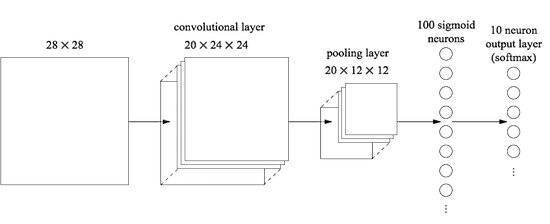
\includegraphics[width=0.917\textwidth]{images/simple_conv.png}
\end{center}

\noindent 在这个架构中，我们可以把卷积层和池化层看作是在学习输入训练图像的局部空间结构，而后面更靠后的全连接层则在更抽象的层次上学习，整合来自整个图像的全局信息. 这是卷积神经网络中一种常见的模式.

让我们训练这样一个网络，看看它的表现如何*\footnote{我在这里继续使用了小批量大小 $10$. 事实上，正如我们之前讨论的，使用更大的小批量可能可以加速训练. 我继续使用相同的小批量大小主要是为了与前面章节的实验保持一致.}:

\begin{lstlisting}
>>> net = Network([
        ConvPoolLayer(image_shape=(mini_batch_size, 1, 28, 28),
                      filter_shape=(20, 1, 5, 5),
                      poolsize=(2, 2)),
        FullyConnectedLayer(n_in=20*12*12, n_out=100),
        SoftmaxLayer(n_in=100, n_out=10)], mini_batch_size)
>>> net.SGD(training_data, 60, mini_batch_size, 0.1,
            validation_data, test_data)

\end{lstlisting}

这样我们就达到了 $98.78$ 百分比的准确率，这比我们之前任何结果都有了相当大的改进. 确实，我们把错误率降低了超过三分之一，这是一个很大的改进.

在指定网络结构时，我把卷积层和池化层当作一个单一的层. 它们是被视为单独的层还是单一的层，在某种程度上是个人偏好的问题. \texttt{network3.py} 把它们当作一个单一的层，因为这样可以使 \texttt{network3.py} 的代码更紧凑一些. 然而，如果需要的话，很容易修改 \texttt{network3.py} 使这些层可以被分别指定.

\begin{exerciseBox}{练习}

\begin{itemize}

\item 如果你省略全连接层，只使用卷积-池化层和 softmax 层，你会得到什么样的分类准确率？包含全连接层有帮助吗？

\end{itemize}

我们能否在 $98.78$ 百分比的分类准确率基础上进一步改进呢？

让我们尝试插入第二个卷积-池化层. 我们将把它插入到现有的卷积-池化层和全连接隐藏层之间. 同样，我们将使用 $5 \times 5$ 的局部感受野，并在 $2 \times 2$ 的区域上进行池化. 让我们看看使用与之前类似的超参数训练时会发生什么：

\begin{lstlisting}
>>> net = Network([
        ConvPoolLayer(image_shape=(mini_batch_size, 1, 28, 28),
                      filter_shape=(20, 1, 5, 5),
                      poolsize=(2, 2)),
        ConvPoolLayer(image_shape=(mini_batch_size, 20, 12, 12),
                      filter_shape=(40, 20, 5, 5),
                      poolsize=(2, 2)),
        FullyConnectedLayer(n_in=40*4*4, n_out=100),
        SoftmaxLayer(n_in=100, n_out=10)], mini_batch_size)
>>> net.SGD(training_data, 60, mini_batch_size, 0.1,
            validation_data, test_data)

\end{lstlisting}

又一次，我们得到了改进：我们现在达到了 $99.06$ 百分比的分类准确率！

在这一点上，有两个自然的问题要问. 第一个问题是：应用第二个卷积-池化层到底意味着什么？事实上，你可以把第二个卷积-池化层的输入看作是 $12 \times 12$ 的``图像''，其``像素''表示原始输入图像中特定局部化特征的存在（或缺失）. 所以你可以把这一层看作是以原始输入图像的一个版本作为输入. 那个版本是抽象化和浓缩过的，但仍然具有大量的空间结构，因此使用第二个卷积-池化层是有意义的.

这是一个令人满意的观点，但它引出了第二个问题. 前一层的输出涉及 $20$ 个独立的特征图，因此第二个卷积-池化层有 $20 \times 12 \times 12$ 个输入. 这就好像我们有 $20$ 个独立的图像输入到卷积-池化层，而不是像第一个卷积-池化层那样只有一个图像. 第二个卷积-池化层中的神经元应该如何响应这些多个输入图像呢？事实上，我们将允许这一层中的每个神经元从其局部感受野中的\emph{所有} $20 \times 5 \times 5$ 个输入神经元学习. 更非正式地说：第二个卷积-池化层中的特征检测器可以访问前一层的\emph{所有}特征，但仅限于它们特定的局部感受野内*\footnote{如果输入图像是彩色的，这个问题在第一个层中就会出现. 在那种情况下，每个像素会有 3 个输入特征，对应于输入图像中的红、绿、蓝通道. 所以我们会允许特征检测器访问所有颜色信息，但仅限于给定的局部感受野内.}.

\end{exerciseBox}

\begin{exerciseBox}{习题}

\begin{itemize}

\item \textbf{使用 tanh 激活函数} 在本书前面的几个地方，我提到过 tanh 函数可能是比 S 型函数更好的激活函数的论点. 我们从未按照那些建议去做，因为我们在使用 S 型函数时已经取得了足够的进展. 但现在让我们尝试一些使用 tanh 作为激活函数的实验. 尝试在卷积层和全连接层中使用 tanh 激活函数来训练网络*\footnote{注意你可以将 \texttt{activation\_\allowbreak{}fn=tanh} 作为参数传递给 \texttt{ConvPoolLayer} 和 \texttt{FullyConnectedLayer} 类.}. 从与 S 型网络相同的超参数开始，但训练 $20$ 个轮次而不是 $60$ 个. 你的网络表现如何？如果你继续训练到 $60$ 个轮次呢？尝试绘制基于 tanh 和基于 S 型的网络在每个轮次的验证准确率，一直到 $60$ 个轮次. 如果你的结果与我的相似，你会发现 tanh 网络训练得稍快一些，但最终准确率非常相似. 你能解释为什么 tanh 网络可能训练得更快吗？你能用 S 型函数获得类似的训练速度吗，也许通过改变学习率，或者做一些重新缩放*\footnote{你也许可以从回忆 $\sigma(z) = (1+\tanh(z/2))/2$ 中获得灵感.}？尝试对学习超参数或网络架构进行半打迭代，寻找 tanh 可能优于 S 型函数的方法. \emph{注意：这是一个开放性问题. 就我个人而言，我没有发现切换到 tanh 有多大优势，尽管我还没有进行详尽的实验，也许你可能会找到一种方法. 无论如何，稍后我们会发现切换到修正线性激活函数的优势，所以我们不会更深入地探讨 tanh 的使用.}

\end{itemize}

\textbf{使用修正线性单元：} 我们在这一点上开发的网络实际上是 1998 年那篇引入 MNIST 问题的开创性论文*\footnote{``Gradient-based learning applied to document recognition''，作者为 Yann LeCun, Léon Bottou, Yoshua Bengio，和 Patrick Haffner (1998). 在细节上有很多差异，但大致来说我们的网络与论文中描述的网络非常相似.}中使用的网络之一的一个变体，那个网络被称为 LeNet-5. 它是进一步实验以及建立理解和直觉的良好基础. 特别是，我们可以通过许多方式改变网络来尝试改进我们的结果.

作为一个开始，让我们改变我们的神经元，使其不使用 S 型激活函数，而是使用修正线性单元. 也就是说，我们将使用激活函数 $f(z) \equiv \max(0, z)$. 我们将训练 $60$ 个轮次，学习率为 $\eta = 0.03$. 我还发现使用一些 l2 正则化有一点帮助，正则化参数 $\lambda = 0.1$:

\begin{lstlisting}
>>> from network3 import ReLU
>>> net = Network([
        ConvPoolLayer(image_shape=(mini_batch_size, 1, 28, 28),
                      filter_shape=(20, 1, 5, 5),
                      poolsize=(2, 2),
                      activation_fn=ReLU),
        ConvPoolLayer(image_shape=(mini_batch_size, 20, 12, 12),
                      filter_shape=(40, 20, 5, 5),
                      poolsize=(2, 2),
                      activation_fn=ReLU),
        FullyConnectedLayer(n_in=40*4*4, n_out=100, activation_fn=ReLU),
        SoftmaxLayer(n_in=100, n_out=10)], mini_batch_size)
>>> net.SGD(training_data, 60, mini_batch_size, 0.03,
            validation_data, test_data, lmbda=0.1)

\end{lstlisting}

我获得了 $99.23$ 百分比的分类准确率. 这比 S 型函数的结果（$99.06$）有适度的改进. 然而，在我所有的实验中，我发现基于修正线性单元的网络始终优于基于 S 型激活函数的网络. 对于这个问题，转向修正线性单元似乎有真正的增益.

是什么使得修正线性激活函数比 S 型函数或 tanh 函数更好呢？目前，我们对这个问题的答案理解得很差. 确实，修正线性单元只是在过去几年才开始被广泛使用. 最近被采用的原因是经验性的：一些人尝试了修正线性单元，通常是基于直觉或启发式论证*\footnote{一个常见的理由是 $\max(0, z)$ 在 $z$ 很大时不会饱和，不像 S 型神经元，这有助于修正线性单元继续学习. 这个论证就其本身而言是好的，但它很难说是一个详细的论证，更像是一个想当然的故事. 注意我们在第 2 章讨论过饱和的问题.}. 他们在基准数据集分类上获得了好的结果，这种做法就传播开来了. 在一个理想的世界里，我们会有一个理论告诉我们对于哪种应用应该选择哪种激活函数. 但目前我们离这样的世界还很远. 如果通过更好的激活函数选择能够获得进一步的重大改进，我一点也不会感到惊讶. 我也期望在未来几十年里，一个强大的激活函数理论会被发展出来. 今天，我们仍然不得不依赖理解不足的经验法则和经验. \textbf{扩展训练数据：} 我们可能希望改进结果的另一种方法是通过算法扩展训练数据. 一种简单的扩展训练数据的方法是将每个训练图像平移一个像素，要么向上一个像素，向下一个像素，向左一个像素，或向右一个像素. 我们可以通过在 shell 提示符下运行程序 \texttt{expand\_\allowbreak{}mnist.py} 来做到这一点*\footnote{\texttt{expand\_\allowbreak{}mnist.py} 的代码可以在这里找到.}:

\begin{lstlisting}

$ python expand_mnist.py

\end{lstlisting}

运行这个程序会读取 $50,000$ 个 MNIST 训练图像，并准备一个扩展的训练集，包含 $250,000$ 个训练图像. 然后我们可以使用那些训练图像来训练我们的网络. 我们将使用与上面相同的网络，带有修正线性单元. 在我最初的实验中，我减少了训练轮次的数量——这是有道理的，因为我们用 $5$ 倍的数据进行训练. 但事实上，扩展数据结果大大减少了过拟合的影响. 因此，经过一些实验后，我最终回到了训练 $60$ 个轮次. 无论如何，让我们训练：

\begin{lstlisting}
>>> expanded_training_data, _, _ = network3.load_data_shared(
        "../data/mnist_expanded.pkl.gz")
>>> net = Network([
        ConvPoolLayer(image_shape=(mini_batch_size, 1, 28, 28),
                      filter_shape=(20, 1, 5, 5),
                      poolsize=(2, 2),
                      activation_fn=ReLU),
        ConvPoolLayer(image_shape=(mini_batch_size, 20, 12, 12),
                      filter_shape=(40, 20, 5, 5),
                      poolsize=(2, 2),
                      activation_fn=ReLU),
        FullyConnectedLayer(n_in=40*4*4, n_out=100, activation_fn=ReLU),
        SoftmaxLayer(n_in=100, n_out=10)], mini_batch_size)
>>> net.SGD(expanded_training_data, 60, mini_batch_size, 0.03,
            validation_data, test_data, lmbda=0.1)

\end{lstlisting}

使用扩展的训练数据，我获得了 $99.37$ 百分比的训练准确率. 所以这个几乎微不足道的变化带来了分类准确率的显著改进. 确实，正如我们之前讨论的，这种通过算法扩展数据的想法可以进一步推进. 只是为了提醒你之前讨论中一些结果的风味： 2003 年， Simard, Steinkraus 和 Platt*\footnote{Best Practices for Convolutional Neural Networks Applied to Visual Document Analysis，作者为 Patrice Simard, Dave Steinkraus，和 John Platt (2003).}使用一个在其他方面与我们的网络非常相似的神经网络，使用两个卷积-池化层，后面跟着一个包含 $100$ 个神经元的隐藏全连接层，将他们的 MNIST 性能提高到了 $99.6$ 百分比. 他们的架构在细节上有一些差异——例如，他们没有使用修正线性单元的优势——但他们改进性能的关键是扩展训练数据. 他们通过旋转、平移和倾斜 MNIST 训练图像来做到这一点. 他们还开发了一个``弹性扭曲''的过程，一种模拟人写字时手部肌肉经历的随机振荡的方法. 通过结合所有这些过程，他们大幅增加了训练数据的有效大小，这就是他们达到 $99.6$ 百分比准确率的方式.

\end{exerciseBox}
\begin{exerciseBox}{习题}

\begin{itemize}

\item 卷积层的理念是在图像上以不变的方式行事. 那么，当我们所做的只是平移输入数据时，我们的网络却能学到更多，这似乎令人惊讶. 你能解释为什么这实际上相当合理吗？

\end{itemize}

\textbf{插入一个额外的全连接层：} 我们能做得更好吗？一种可能是使用与上面完全相同的步骤，但扩大全连接层的规模. 我尝试了 $300$ 和 $1,000$ 个神经元，分别得到 $99.46$ 和 $99.43$ 百分比的结果. 这很有趣，但并不是对先前结果 ($99.37$ 百分比) 真正令人信服的超越.

那添加一个额外的全连接层呢？让我们尝试插入一个额外的全连接层，这样我们就有两个 $100$ 个隐藏神经元的全连接层：

\begin{lstlisting}
>>> net = Network([
        ConvPoolLayer(image_shape=(mini_batch_size, 1, 28, 28),
                      filter_shape=(20, 1, 5, 5),
                      poolsize=(2, 2),
                      activation_fn=ReLU),
        ConvPoolLayer(image_shape=(mini_batch_size, 20, 12, 12),
                      filter_shape=(40, 20, 5, 5),
                      poolsize=(2, 2),
                      activation_fn=ReLU),
        FullyConnectedLayer(n_in=40*4*4, n_out=100, activation_fn=ReLU),
        FullyConnectedLayer(n_in=100, n_out=100, activation_fn=ReLU),
        SoftmaxLayer(n_in=100, n_out=10)], mini_batch_size)
>>> net.SGD(expanded_training_data, 60, mini_batch_size, 0.03,
            validation_data, test_data, lmbda=0.1)

\end{lstlisting}

这样做，我得到了 $99.43$ 百分比的测试准确率. 同样，扩展后的网络并没有太大帮助. 用包含 $300$ 和 $1,000$ 个神经元的全连接层进行类似的实验，得到的结果分别为 $99.48$ 和 $99.47$ 百分比. 这令人鼓舞，但仍未达到真正决定性的超越.

这里发生了什么？是扩展的或额外的全连接层对 MNIST 真的没有帮助吗？还是我们的网络有能力做得更好，但我们学习的方式不对？例如，也许我们可以使用更强的正则化技术来减少过拟合的倾向. 一种可能是第 3 章介绍的 dropout 技术. 回想一下， dropout 的基本思想是在训练网络时随机移除单个激活值. 这使得模型对单个证据的丢失更加鲁棒，从而不太可能依赖于训练数据的特定特性. 让我们尝试将 dropout 应用于最后的全连接层：

\begin{lstlisting}
>>> net = Network([
        ConvPoolLayer(image_shape=(mini_batch_size, 1, 28, 28),
                      filter_shape=(20, 1, 5, 5),
                      poolsize=(2, 2),
                      activation_fn=ReLU),
        ConvPoolLayer(image_shape=(mini_batch_size, 20, 12, 12),
                      filter_shape=(40, 20, 5, 5),
                      poolsize=(2, 2),
                      activation_fn=ReLU),
        FullyConnectedLayer(
            n_in=40*4*4, n_out=1000, activation_fn=ReLU, p_dropout=0.5),
        FullyConnectedLayer(
            n_in=1000, n_out=1000, activation_fn=ReLU, p_dropout=0.5),
        SoftmaxLayer(n_in=1000, n_out=10, p_dropout=0.5)],
        mini_batch_size)
>>> net.SGD(expanded_training_data, 40, mini_batch_size, 0.03,
            validation_data, test_data)

\end{lstlisting}

使用这个，我们获得了 $99.60$ 百分比的准确率，这比我们之前的结果有了实质性的改进，尤其是我们的主要基准，即具有 $100$ 个隐藏神经元的网络，我们达到了 $99.37$ 百分比.

有两个变化值得注意.

首先，我将训练轮次减少到 $40$: dropout 减少了过拟合，因此我们学得更快.

其次，全连接隐藏层有 $1,000$ 个神经元，而不是之前使用的 $100$ 个. 当然， dropout 在训练时有效地省略了许多神经元，所以一些扩展是意料之中的. 事实上，我尝试了 $300$ 和 $1,000$ 个隐藏神经元的实验，并在 $1,000$ 个隐藏神经元上获得了 (非常轻微地) 更好的验证性能. \textbf{使用网络集成：} 进一步提高性能的一个简单方法是创建几个神经网络，然后让它们投票来确定最佳分类. 例如，假设我们使用上面的方案训练了 $5$ 个不同的神经网络，每个都达到了接近 $99.6$ 百分比的准确率. 即使这些网络都具有相似的准确率，由于不同的随机初始化，它们很可能会犯不同的错误. 在我们的 $5$ 个网络中进行投票可能会产生比任何单个网络更好的分类，这是合理的.

这听起来好得令人难以置信，但这种集成是神经网络和其他机器学习技术中常见的技巧. 它确实带来了进一步的改进：我们最终达到了 $99.67$ 百分比的准确率. 换句话说，我们的网络集成正确分类了 $10,000$ 张测试图像中除 $33$ 张之外的所有图像.

测试集中剩余的错误如下所示. 右上角的标签是根据 MNIST 数据的正确分类，而右下角是我们网络集成的输出标签：

\begin{center}
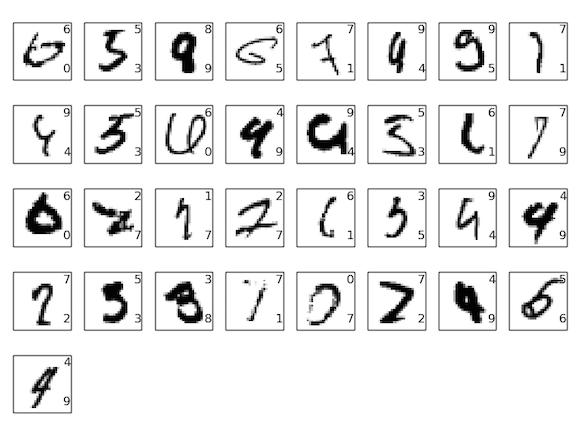
\includegraphics[width=0.967\textwidth]{images/ensemble_errors.png}
\end{center}

\noindent 值得详细查看这些. 前两个数字，一个 6 和一个 5，是我们集成的真实错误. 然而，它们也是可以理解的错误，是人类可能犯的那种错误. 那个 6 看起来确实很像 0，而 5 看起来很像 3. 第三张图像，据说是 8，实际上在我看来更像 9. 所以我在这里支持网络集成：我认为它比最初绘制数字的人做得更好. 另一方面，第四张图像，那个 6，确实似乎被我们的网络分类得很差.

以此类推. 在大多数情况下，我们网络的选择似乎至少是合理的，在某些情况下，它们在分类方面比最初写数字的人做得更好. 总的来说，我们的网络提供了卓越的性能，尤其是当你考虑到它们正确分类了未显示的 9,967 张图像时. 在这种背景下，这里少数明显的错误似乎相当可以理解. 即使是细心的人也会偶尔犯错. 因此，我预计只有极其细心和有条理的人才能做得更好. 我们的网络正在接近人类的表现. \textbf{为什么我们只对全连接层应用 dropout:} 如果你仔细查看上面的代码，你会注意到我们只对网络的全连接部分应用了 dropout，而不是卷积层. 原则上我们可以对卷积层应用类似的过程. 但实际上，没有必要：卷积层具有相当大的内置抗过拟合能力. 原因是共享权重意味着卷积滤波器被迫从整个图像中学习. 这使得它们不太可能捕捉到训练数据中的局部特性. 因此，不太需要应用其他正则化器，如 dropout. \textbf{更进一步：} 在 MNIST 上进一步提高性能是可能的. Rodrigo Benenson 编制了一个信息丰富的摘要页面，展示了多年来的进展，并附有论文链接. 这些论文中的许多都使用深度卷积网络，其思路与我们一直使用的网络类似. 如果你深入研究这些论文，你会发现许多有趣的技术，你可能会喜欢实现其中的一些. 如果你这样做，明智的做法是从一个可以快速训练的简单网络开始实现，这将帮助你更快地理解正在发生的事情.

在大多数情况下，我不会尝试综述这些最近的工作. 但我忍不住要做一个例外. 这是 Cireșan, Meier, Gambardella 和 Schmidhuber 在 2010 年的一篇论文*\footnote{Deep, Big, Simple Neural Nets Excel on Handwritten Digit Recognition, by Dan Claudiu Cireșan, Ueli Meier, Luca Maria Gambardella, and Jürgen Schmidhuber (2010).}. 我喜欢这篇论文的地方在于它多么简单. 该网络是一个多层神经网络，仅使用全连接层 (没有卷积). 他们最成功的网络隐藏层分别包含 $2,500$, $2,000$, $1,500$, $1,000$ 和 $500$ 个神经元. 他们使用类似于 Simard \emph{et al} 的想法来扩展他们的训练数据. 但除此之外，他们很少使用其他技巧，包括没有卷积层：这是一个普通的、香草味的网络，如果有足够的计算能力，只要有足够的耐心，在 1980 年代就可以训练出来 (如果 MNIST 数据集存在的话). 他们实现了 $99.65$ 百分比的分类准确率，或多或少与我们相同. 关键是使用一个非常大、非常深的网络，并使用 GPU 来加速训练. 这让他们能够训练许多轮次. 他们还利用他们长时间的训练逐渐将学习率从 $10^{-3}$ 降低到 $10^{-6}$. 尝试使用类似他们的架构来匹配这些结果是一个有趣的练习. \textbf{为什么我们能够训练？} 我们在上一章看到，在深层的多层神经网络中训练存在根本性的障碍. 特别是，我们看到梯度往往相当不稳定：当我们从输出层移动到较早的层时，梯度往往会消失 (梯度消失问题) 或爆炸 (梯度爆炸问题). 由于梯度是我们用来训练的信号，这会导致问题.

我们是如何避免这些结果的？

当然，答案是我们并没有避免这些结果. 相反，我们做了一些帮助我们无论如何都能继续的事情. 特别是： (1) 使用卷积层大大减少了这些层中的参数数量，使学习问题容易得多； (2) 使用更强大的正则化技术 (特别是 dropout 和卷积层) 来减少过拟合，这在更复杂的网络中否则是更大的问题； (3) 使用修正线性单元而不是 S 型神经元，以加速训练 - 根据经验，通常加快 $3$-$5$ 倍； (4) 使用 GPU 并愿意长时间训练. 特别是，在我们最后的实验中，我们使用比原始 MNIST 训练数据大 $5$ 倍的数据集训练了 $40$ 轮次. 在本书的早期，我们主要只使用原始训练数据训练 $30$ 轮次. 结合因素 (3) 和 (4)，就好像我们训练的时间比以前长了大约 $30$ 倍.

你的回答可能是 ``就这样吗？这就是我们训练深度网络所需要做的全部吗？有什么好大惊小怪的？''

当然，我们也使用了其他想法：利用足够大的数据集 (以帮助避免过拟合)；使用正确的代价函数 (以避免学习减慢)；使用良好的权重初始化 (也是为了避免学习减慢，由于神经元饱和)；通过算法扩展训练数据. 我们在前面的章节中讨论了这些和其他想法，并且在本章中大多能够在很少评论的情况下重用这些想法.

话虽如此，这确实是一组相当简单的想法. 简单，但协同使用时很强大. 开始深度学习已经变得相当容易了！ \textbf{这些网络到底有多深？} 将卷积-池化层计为单层，我们的最终架构有 $4$ 个隐藏层. 这样的网络真的配得上被称为\emph{深度}网络吗？当然， $4$ 个隐藏层比我们之前研究的浅层网络多得多. 那些网络大多只有一个隐藏层，或者偶尔有 $2$ 个隐藏层. 另一方面，截至 2015 年，最先进的深度网络有时有几十个隐藏层. 我偶尔听到人们采取比你更深的姿态，认为如果你在隐藏层数量上没有跟上潮流，那么你就不是真正在做深度学习. 我不认同这种态度，部分原因是它使深度学习的定义变成了依赖于当下结果的东西. 深度学习的真正突破是认识到超越在 2000 年代中期之前主导工作的浅层 $1$- 和 $2$-隐藏层网络是可行的. 这确实是一个重大的突破，开启了对更具表现力的模型的探索. 但除此之外，层数并不是主要的基本兴趣所在. 相反，使用更深的网络是一种工具，用于帮助实现其他目标 - 比如更好的分类准确率. \textbf{关于过程的一点说明：} 在本节中，我们已经顺利地从单隐藏层浅层网络过渡到多层卷积网络. 这一切看起来如此容易！我们做一个改变，并且在大多数情况下，我们得到了改进. 如果你开始实验，我可以保证事情不会总是那么顺利. 原因是我呈现了一个经过清理的叙述，省略了许多实验 - 包括许多失败的实验. 这个经过清理的叙述有望帮助你清楚地了解基本想法. 但它也有传达不完整印象的风险. 获得一个好的、可工作的网络可能涉及大量的试错，以及偶尔的挫折. 在实践中，你应该预期会进行相当多的实验. 为了加快这个过程，你可能会发现重新审视第 3 章关于如何选择神经网络超参数的讨论很有帮助，也许还可以看看该节中建议的一些进一步阅读.

\end{exerciseBox}
\sectionTitle{卷积网络的代码}{卷积网络的代码}

好的，让我们来看看我们程序的代码，\texttt{network3.py}. 在结构上，它类似于我们在第 3 章开发的程序 \texttt{network2.py}，尽管由于使用了 Theano，细节有所不同. 我们将从 \texttt{FullyConnectedLayer} 类开始看起，它类似于本书前面研究过的层. 代码如下（讨论见后）*\footnote{2016 年 11 月注：几位读者指出，在初始化 \texttt{self.w} 的那一行，我设置了 \texttt{scale=np.sqrt(1.0/n\_\allowbreak{}out)}，而第 3 章的论证表明更好的初始化可能是 \texttt{scale=np.sqrt(1.0/n\_\allowbreak{}in)}. 这纯粹是我的一个错误. 在理想情况下，我会用正确的代码重新运行本章的所有示例. 不过，我已经转向了其他项目，所以就让这个错误保留吧.}：

\begin{lstlisting}
class FullyConnectedLayer(object):

    def __init__(self, n_in, n_out, activation_fn=sigmoid, p_dropout=0.0):
        self.n_in = n_in
        self.n_out = n_out
        self.activation_fn = activation_fn
        self.p_dropout = p_dropout
        # Initialize weights and biases
        self.w = theano.shared(
            np.asarray(
                np.random.normal(
                    loc=0.0, scale=np.sqrt(1.0/n_out), size=(n_in, n_out)),
                dtype=theano.config.floatX),
            name='w', borrow=True)
        self.b = theano.shared(
            np.asarray(np.random.normal(loc=0.0, scale=1.0, size=(n_out,)),
                       dtype=theano.config.floatX),
            name='b', borrow=True)
        self.params = [self.w, self.b]

    def set_inpt(self, inpt, inpt_dropout, mini_batch_size):
        self.inpt = inpt.reshape((mini_batch_size, self.n_in))
        self.output = self.activation_fn(
            (1-self.p_dropout)*T.dot(self.inpt, self.w) + self.b)
        self.y_out = T.argmax(self.output, axis=1)
        self.inpt_dropout = dropout_layer(
            inpt_dropout.reshape((mini_batch_size, self.n_in)), self.p_dropout)
        self.output_dropout = self.activation_fn(
            T.dot(self.inpt_dropout, self.w) + self.b)

    def accuracy(self, y):
        "Return the accuracy for the mini-batch."
        return T.mean(T.eq(y, self.y_out))

\end{lstlisting}

\texttt{\_\allowbreak{}\_\allowbreak{}init\_\allowbreak{}\_\allowbreak{}} 方法的大部分内容不言自明，但有几句话可能有助于阐明代码. 按照惯例，我们将权重和偏置随机初始化为具有适当标准差的正态随机变量. 执行此操作的代码行看起来有点吓人. 然而，大部分复杂性只是将权重和偏置加载到 Theano 所称的共享变量中. 这确保了这些变量可以在 GPU 上处理，如果有可用的 GPU 的话. 我们不会过多深入细节. 如果你感兴趣，可以深入研究 Theano 文档. 另请注意，这种权重和偏置初始化是为 S 型激活函数设计的（如前所述）. 理想情况下，对于 tanh 和修正线性函数等激活函数，我们会以略有不同的方式初始化权重和偏置. 这将在下面的习题中进一步讨论.\texttt{\_\allowbreak{}\_\allowbreak{}init\_\allowbreak{}\_\allowbreak{}} 方法以 \texttt{self.params = [self.w, self.b]} 结束. 这是一种便捷的方式，用于捆绑与该层相关的所有可学习参数. 稍后，\texttt{Network.SGD} 方法将使用 \texttt{params} 属性来确定 \texttt{Network} 实例中哪些变量可以学习.

\texttt{set\_\allowbreak{}inpt} 方法用于设置层的输入，并计算相应的输出. 我使用名称 \texttt{inpt} 而不是 \texttt{input}，因为 \texttt{input} 是 Python 的内置函数，而干扰内置函数往往会导致不可预测的行为和难以诊断的错误. 请注意，我们实际上以两种不同的方式设置输入：作为 \texttt{self.inpt} 和 \texttt{self.inpt\_\allowbreak{}dropout}. 这样做是因为在训练期间我们可能想要使用 dropout. 如果是这种情况，那么我们希望移除比例为 \texttt{self.p\_\allowbreak{}dropout} 的神经元. 这就是 \texttt{set\_\allowbreak{}inpt} 方法倒数第二行中的函数 \texttt{dropout\_\allowbreak{}layer} 所做的. 因此，\texttt{self.inpt\_\allowbreak{}dropout} 和 \texttt{self.output\_\allowbreak{}dropout} 在训练期间使用，而 \texttt{self.inpt} 和 \texttt{self.output} 用于所有其他目的，例如，评估验证数据和测试数据上的准确率.

\texttt{ConvPoolLayer} 和 \texttt{SoftmaxLayer} 类的定义与 \texttt{FullyConnectedLayer} 类似. 事实上，它们如此接近，以至于我不会在这里摘录代码. 如果你感兴趣，可以查看本节后面 \texttt{network3.py} 的完整列表.

然而，一些细节上的微小差异值得一提. 最明显的是，在 \texttt{ConvPoolLayer} 和 \texttt{SoftmaxLayer} 中，我们以适合该层类型的方式计算输出激活值. 幸运的是，Theano 使这变得容易，提供了内置操作来计算卷积、最大池化和 softmax 函数.

不太明显的是，当我们引入 softmax 层时，我们从未讨论过如何初始化权重和偏置. 在其他地方，我们论证过对于 S 型层，我们应该使用适当参数化的正态随机变量来初始化权重. 但那个启发式论证是特定于 S 型神经元的（并且，经过一些修正，也适用于 tanh 神经元）. 然而，没有特别的理由认为该论证应该适用于 softmax 层. 因此，没有\emph{先验}理由再次应用该初始化. 与其这样做，我将所有

好的，我们已经看过了所有的层类. 那么 \texttt{Network} 类呢？让我们从 \texttt{\_\allowbreak{}\_\allowbreak{}init\_\allowbreak{}\_\allowbreak{}} 方法开始看起：

\begin{lstlisting}
class Network(object):

    def __init__(self, layers, mini_batch_size):
        """Takes a list of `layers`, describing the network architecture, and
        a value for the `mini_batch_size` to be used during training
        by stochastic gradient descent.

        """
        self.layers = layers
        self.mini_batch_size = mini_batch_size
        self.params = [param for layer in self.layers for param in layer.params]
        self.x = T.matrix("x")
        self.y = T.ivector("y")
        init_layer = self.layers[0]
        init_layer.set_inpt(self.x, self.x, self.mini_batch_size)
        for j in xrange(1, len(self.layers)):
            prev_layer, layer  = self.layers[j-1], self.layers[j]
            layer.set_inpt(
                prev_layer.output, prev_layer.output_dropout, self.mini_batch_size)
        self.output = self.layers[-1].output
        self.output_dropout = self.layers[-1].output_dropout

\end{lstlisting}

这里的大部分内容不言自明，或者几乎如此.\texttt{self.params = [param for layer in...]} 这一行将每一层的参数捆绑到一个列表中. 正如上面所预期的，\texttt{Network.SGD} 方法将使用 \texttt{self.params} 来确定 \texttt{Network} 中哪些变量可以学习.\texttt{self.x = T.matrix(``x'')} 和 \texttt{self.y = T.ivector(``y'')} 这两行定义了名为 \texttt{x} 和 \texttt{y} 的 Theano 符号变量. 这些将用于表示网络的输入和期望输出.

现在，这不是一篇 Theano 教程，因此我们不会过于深入地探讨这些符号变量意味着什么*\footnote{Theano 文档提供了对 Theano 的良好介绍. 如果你遇到困难，查看网上其他可用的教程之一可能会有所帮助. 例如，本教程涵盖了许多基础知识.}. 但大致的想法是，它们代表数学变量，\emph{而非}显式的值. 我们可以对这些变量做所有通常可以做的事情：加、减、乘它们，应用函数，等等. 事实上，Theano 提供了许多操作这类符号变量的方法，比如做卷积、最大池化等等. 但最大的优势是能够使用一种非常通用的反向传播算法形式来进行快速的符号微分. 这对于将随机梯度下降应用于各种各样的网络架构极为有用. 特别是，接下来的几行代码定义了网络的符号输出. 我们首先设置初始层的输入，代码如下：

\begin{lstlisting}
        init_layer.set_inpt(self.x, self.x, self.mini_batch_size)

\end{lstlisting}

请注意，输入是一次一个小批量设置的，这就是小批量大小存在的原因. 另请注意，我们将输入 \texttt{self.x} 传递了两次：这是因为我们可能以两种不同的方式使用网络（使用或不使用 dropout）. 然后 \texttt{for} 循环将符号变量 \texttt{self.x} 向前传播通过 \texttt{Network} 的各层. 这允许我们定义最终的 \texttt{output} 和 \texttt{output\_\allowbreak{}dropout} 属性，它们符号化地表示 \texttt{Network} 的输出.

现在我们已经理解了 \texttt{Network} 是如何初始化的，让我们看看它是如何训练的，即使用 \texttt{SGD} 方法. 代码看起来很长，但其结构实际上相当简单. 代码后面有解释性注释.

\begin{lstlisting}
    def SGD(self, training_data, epochs, mini_batch_size, eta,
            validation_data, test_data, lmbda=0.0):
        """Train the network using mini-batch stochastic gradient descent."""
        training_x, training_y = training_data
        validation_x, validation_y = validation_data
        test_x, test_y = test_data

        # compute number of minibatches for training, validation and testing
        num_training_batches = size(training_data)/mini_batch_size
        num_validation_batches = size(validation_data)/mini_batch_size
        num_test_batches = size(test_data)/mini_batch_size

        # define the (regularized) cost function, symbolic gradients, and updates
        l2_norm_squared = sum([(layer.w**2).sum() for layer in self.layers])
        cost = self.layers[-1].cost(self)+\
               0.5*lmbda*l2_norm_squared/num_training_batches
        grads = T.grad(cost, self.params)
        updates = [(param, param-eta*grad)
                   for param, grad in zip(self.params, grads)]

        # define functions to train a mini-batch, and to compute the
        # accuracy in validation and test mini-batches.
        i = T.lscalar() # mini-batch index
        train_mb = theano.function(
            [i], cost, updates=updates,
            givens={
                self.x:
                training_x[i*self.mini_batch_size: (i+1)*self.mini_batch_size],
                self.y:
                training_y[i*self.mini_batch_size: (i+1)*self.mini_batch_size]
            })
        validate_mb_accuracy = theano.function(
            [i], self.layers[-1].accuracy(self.y),
            givens={
                self.x:
                validation_x[i*self.mini_batch_size: (i+1)*self.mini_batch_size],
                self.y:
                validation_y[i*self.mini_batch_size: (i+1)*self.mini_batch_size]
            })
        test_mb_accuracy = theano.function(
            [i], self.layers[-1].accuracy(self.y),
            givens={
                self.x:
                test_x[i*self.mini_batch_size: (i+1)*self.mini_batch_size],
                self.y:
                test_y[i*self.mini_batch_size: (i+1)*self.mini_batch_size]
            })
        self.test_mb_predictions = theano.function(
            [i], self.layers[-1].y_out,
            givens={
                self.x:
                test_x[i*self.mini_batch_size: (i+1)*self.mini_batch_size]
            })
        # Do the actual training
        best_validation_accuracy = 0.0
        for epoch in xrange(epochs):
            for minibatch_index in xrange(num_training_batches):
                iteration = num_training_batches*epoch+minibatch_index
                if iteration
                    print("Training mini-batch number {0}".format(iteration))
                cost_ij = train_mb(minibatch_index)
                if (iteration+1)
                    validation_accuracy = np.mean(
                        [validate_mb_accuracy(j) for j in xrange(num_validation_batches)])
                    print("Epoch {0}: validation accuracy {1:.2
                        epoch, validation_accuracy))
                    if validation_accuracy >= best_validation_accuracy:
                        print("This is the best validation accuracy to date.")
                        best_validation_accuracy = validation_accuracy
                        best_iteration = iteration
                        if test_data:
                            test_accuracy = np.mean(
                                [test_mb_accuracy(j) for j in xrange(num_test_batches)])
                            print('The corresponding test accuracy is {0:.2
                                test_accuracy))
        print("Finished training network.")
        print("Best validation accuracy of {0:.2
            best_validation_accuracy, best_iteration))
        print("Corresponding test accuracy of {0:.2

\end{lstlisting}

前几行很直接，将数据集分为 $x$ 和 $y$ 分量，并计算每个数据集中使用的小批量的数量. 接下来的几行更有趣，展示了 Theano 使用起来有趣的一些方面. 让我们在这里明确摘录这些行：
\begin{lstlisting}
        # define the (regularized) cost function, symbolic gradients, and updates
        l2_norm_squared = sum([(layer.w**2).sum() for layer in self.layers])
        cost = self.layers[-1].cost(self)+\
               0.5*lmbda*l2_norm_squared/num_training_batches
        grads = T.grad(cost, self.params)
        updates = [(param, param-eta*grad)
                   for param, grad in zip(self.params, grads)]

\end{lstlisting}

在这些代码行中，我们以符号方式建立了正则化的对数似然代价函数，在梯度函数中计算相应的导数，以及相应的参数更新.Theano 让我们仅用这几行代码就实现了所有这些. 唯一隐藏的是，计算 \texttt{cost} 涉及对输出层的 \texttt{cost} 方法的调用；那段代码在 \texttt{network3.py} 的其他地方. 但那段代码无论如何都很简短. 定义了所有这些之后，就可以定义 \texttt{train\_\allowbreak{}mb} 函数了，这是一个 Theano 符号函数，它使用 \texttt{updates} 来更新 \texttt{Network} 参数，给定一个小批量索引. 类似地，\texttt{validate\_\allowbreak{}mb\_\allowbreak{}accuracy} 和 \texttt{test\_\allowbreak{}mb\_\allowbreak{}accuracy} 计算 \texttt{Network} 在任何给定的验证或测试数据小批量上的准确率. 通过对这些函数取平均，我们将能够计算整个验证和测试数据集上的准确率.

\texttt{SGD} 方法的其余部分不言自明——我们只是遍历轮次，反复在小批量训练数据上训练网络，并计算验证和测试准确率.

好了，我们现在已经理解了 \texttt{network3.py} 中最重要的代码片段. 让我们简要地看一下整个程序. 你不需要详细阅读它，但你可能喜欢浏览一下，也许深入到你感兴趣的任何部分. 真正理解它的最好方法当然是修改它、添加额外功能，或者重构任何你认为可以做得更优雅的地方. 代码之后有一些习题，其中包含一些入门的建议. 以下是代码*\footnote{在 GPU 上使用 Theano 可能有点棘手. 特别是，很容易犯从 GPU 上拉取数据的错误，这会大大降低速度. 我试图避免这一点. 话虽如此，通过仔细优化 Theano 的配置，这段代码肯定还可以进一步加速不少. 更多细节请参阅 Theano 文档.}：

\begin{lstlisting}
"""network3.py
~~~~~~~~~~~~~~

A Theano-based program for training and running simple neural
networks.

Supports several layer types (fully connected, convolutional, max
pooling, softmax), and activation functions (sigmoid, tanh, and
rectified linear units, with more easily added).

When run on a CPU, this program is much faster than network.py and
network2.py.  However, unlike network.py and network2.py it can also
be run on a GPU, which makes it faster still.

Because the code is based on Theano, the code is different in many
ways from network.py and network2.py.  However, where possible I have
tried to maintain consistency with the earlier programs.  In
particular, the API is similar to network2.py.  Note that I have
focused on making the code simple, easily readable, and easily
modifiable.  It is not optimized, and omits many desirable features.

This program incorporates ideas from the Theano documentation on
convolutional neural nets (notably,
http://deeplearning.net/tutorial/lenet.html ), from Misha Denil's
implementation of dropout (https://github.com/mdenil/dropout ), and
from Chris Olah (http://colah.github.io ).

Written for Theano 0.6 and 0.7, needs some changes for more recent
versions of Theano.

"""

#### Libraries
# Standard library
import cPickle
import gzip

# Third-party libraries
import numpy as np
import theano
import theano.tensor as T
from theano.tensor.nnet import conv
from theano.tensor.nnet import softmax
from theano.tensor import shared_randomstreams
from theano.tensor.signal import downsample

# Activation functions for neurons
def linear(z): return z
def ReLU(z): return T.maximum(0.0, z)
from theano.tensor.nnet import sigmoid
from theano.tensor import tanh

#### Constants
GPU = True
if GPU:
    print "Trying to run under a GPU.  If this is not desired, then modify "+\
        "network3.py\nto set the GPU flag to False."
    try: theano.config.device = 'gpu'
    except: pass # it's already set
    theano.config.floatX = 'float32'
else:
    print "Running with a CPU.  If this is not desired, then the modify "+\
        "network3.py to set\nthe GPU flag to True."

#### Load the MNIST data
def load_data_shared(filename="../data/mnist.pkl.gz"):
    f = gzip.open(filename, 'rb')
    training_data, validation_data, test_data = cPickle.load(f)
    f.close()
    def shared(data):
        """Place the data into shared variables.  This allows Theano to copy
        the data to the GPU, if one is available.

        """
        shared_x = theano.shared(
            np.asarray(data[0], dtype=theano.config.floatX), borrow=True)
        shared_y = theano.shared(
            np.asarray(data[1], dtype=theano.config.floatX), borrow=True)
        return shared_x, T.cast(shared_y, "int32")
    return [shared(training_data), shared(validation_data), shared(test_data)]

#### Main class used to construct and train networks
class Network(object):

    def __init__(self, layers, mini_batch_size):
        """Takes a list of `layers`, describing the network architecture, and
        a value for the `mini_batch_size` to be used during training
        by stochastic gradient descent.

        """
        self.layers = layers
        self.mini_batch_size = mini_batch_size
        self.params = [param for layer in self.layers for param in layer.params]
        self.x = T.matrix("x")
        self.y = T.ivector("y")
        init_layer = self.layers[0]
        init_layer.set_inpt(self.x, self.x, self.mini_batch_size)
        for j in xrange(1, len(self.layers)):
            prev_layer, layer  = self.layers[j-1], self.layers[j]
            layer.set_inpt(
                prev_layer.output, prev_layer.output_dropout, self.mini_batch_size)
        self.output = self.layers[-1].output
        self.output_dropout = self.layers[-1].output_dropout

    def SGD(self, training_data, epochs, mini_batch_size, eta,
            validation_data, test_data, lmbda=0.0):
        """Train the network using mini-batch stochastic gradient descent."""
        training_x, training_y = training_data
        validation_x, validation_y = validation_data
        test_x, test_y = test_data

        # compute number of minibatches for training, validation and testing
        num_training_batches = size(training_data)/mini_batch_size
        num_validation_batches = size(validation_data)/mini_batch_size
        num_test_batches = size(test_data)/mini_batch_size

        # define the (regularized) cost function, symbolic gradients, and updates
        l2_norm_squared = sum([(layer.w**2).sum() for layer in self.layers])
        cost = self.layers[-1].cost(self)+\
               0.5*lmbda*l2_norm_squared/num_training_batches
        grads = T.grad(cost, self.params)
        updates = [(param, param-eta*grad)
                   for param, grad in zip(self.params, grads)]

        # define functions to train a mini-batch, and to compute the
        # accuracy in validation and test mini-batches.
        i = T.lscalar() # mini-batch index
        train_mb = theano.function(
            [i], cost, updates=updates,
            givens={
                self.x:
                training_x[i*self.mini_batch_size: (i+1)*self.mini_batch_size],
                self.y:
                training_y[i*self.mini_batch_size: (i+1)*self.mini_batch_size]
            })
        validate_mb_accuracy = theano.function(
            [i], self.layers[-1].accuracy(self.y),
            givens={
                self.x:
                validation_x[i*self.mini_batch_size: (i+1)*self.mini_batch_size],
                self.y:
                validation_y[i*self.mini_batch_size: (i+1)*self.mini_batch_size]
            })
        test_mb_accuracy = theano.function(
            [i], self.layers[-1].accuracy(self.y),
            givens={
                self.x:
                test_x[i*self.mini_batch_size: (i+1)*self.mini_batch_size],
                self.y:
                test_y[i*self.mini_batch_size: (i+1)*self.mini_batch_size]
            })
        self.test_mb_predictions = theano.function(
            [i], self.layers[-1].y_out,
            givens={
                self.x:
                test_x[i*self.mini_batch_size: (i+1)*self.mini_batch_size]
            })
        # Do the actual training
        best_validation_accuracy = 0.0
        for epoch in xrange(epochs):
            for minibatch_index in xrange(num_training_batches):
                iteration = num_training_batches*epoch+minibatch_index
                if iteration
                    print("Training mini-batch number {0}".format(iteration))
                cost_ij = train_mb(minibatch_index)
                if (iteration+1)
                    validation_accuracy = np.mean(
                        [validate_mb_accuracy(j) for j in xrange(num_validation_batches)])
                    print("Epoch {0}: validation accuracy {1:.2
                        epoch, validation_accuracy))
                    if validation_accuracy >= best_validation_accuracy:
                        print("This is the best validation accuracy to date.")
                        best_validation_accuracy = validation_accuracy
                        best_iteration = iteration
                        if test_data:
                            test_accuracy = np.mean(
                                [test_mb_accuracy(j) for j in xrange(num_test_batches)])
                            print('The corresponding test accuracy is {0:.2
                                test_accuracy))
        print("Finished training network.")
        print("Best validation accuracy of {0:.2
            best_validation_accuracy, best_iteration))
        print("Corresponding test accuracy of {0:.2

#### Define layer types

class ConvPoolLayer(
\end{lstlisting}

\chapter*{附录：存在智能的\emph{简单}算法吗？}
\markboth{附录：存在智能的简单算法吗？}{}
\phantomsection
\addcontentsline{toc}{chapter}{附录：存在智能的简单算法吗？}
在本书中，我们关注的是神经网络的细节：它们如何工作，以及如何用它们来解决模式识别问题. 这些内容有许多直接的实际应用. 但是，当然，人们对神经网络感兴趣的一个原因是希望有一天它们能远远超越这些基本的模式识别问题. 也许它们，或者某种其他基于数字计算机的方法，最终会被用来建造会思考的机器，即能够匹敌或超越人类智能的机器？这一设想远远超出了本书所讨论的内容——或者说超出了世界上任何人知道如何做到的范围. 但进行推测是很有趣的.

关于计算机是否\emph{可能}匹敌人类智能，一直存在许多争论. 我不打算参与这个问题. 尽管争论不断，我相信智能计算机是可能的这一点并不存在严重疑问——尽管它可能极其复杂，也许远远超出当前技术——而当前的否定者有一天会看起来很像活力论者.

更确切地说，我在这里探讨的问题是：是否存在一套\emph{简单}的原则可以用来解释智能？具体而言，更实际地说，是否存在一个\emph{智能的简单算法}？

存在真正简单的智能算法这一想法是一个大胆的想法. 它听起来可能过于乐观而不像是真的. 许多人有一种强烈的直觉，认为智能具有相当大的不可约复杂性. 他们对人类思维的惊人多样性和灵活性印象深刻，以至于得出结论：智能的简单算法必定是不可能的. 尽管有这种直觉，我认为匆忙下结论是不明智的. 科学史上充满了这样的例子：一个现象最初看起来极其复杂，但后来被一些简单而有力的思想所解释.

例如，考虑天文学的早期. 人类自古以来就知道天空中有各种各样的物体：太阳、月亮、行星、彗星和恒星. 这些物体的运动方式非常不同——例如，恒星以庄重、规律的方式在天空中移动，而彗星则仿佛凭空出现，划过天空，然后消失. 在 16 世纪，只有愚蠢的乐观主义者才会想象所有这些物体的运动可以用一套简单的原则来解释. 但在 17 世纪，Newton 提出了他的万有引力理论，它不仅解释了所有这些运动，还解释了潮汐和地球上抛射体行为等地面现象.16 世纪的愚蠢乐观主义者回过头来看倒像是悲观主义者，要求的太少了.

当然，科学中还有更多这样的例子. 考虑构成我们世界的无数化学物质，Mendeleev 的元素周期表如此优美地解释了它们，而周期表本身又由几条可以从量子力学中得到的简单规则所解释. 或者生物世界中为何有如此多的复杂性和多样性这一谜题，其起源原来在于自然选择的进化原理. 这些以及许多其他例子表明，仅仅因为我们的头脑——目前智能的最佳范例——所做的\emph{看起来}非常复杂，就排除对智能的简单解释，是不明智的*\footnote{在本附录中，我假设一台计算机要被认定为智能的，其能力必须匹敌或超越人类思维能力. 因此我将问题``存在智能的简单算法吗？''等同于``是否存在一个能够沿着与人类大脑基本相同的思路进行`思考'的简单算法？''然而，值得注意的是，很可能存在一些不包含人类思维、但以有趣的方式超越人类思维的智能形式.}.

相反地，尽管有这些乐观的例子，逻辑上也有可能智能只能由大量根本不同的机制来解释. 就我们的大脑而言，那些许多机制也许是在我们物种的进化历史中响应许多不同的选择压力而进化出来的. 如果这种观点是正确的，那么智能涉及相当大的不可约复杂性，智能的简单算法就是不可能的.

这两种观点哪一种正确？

为了深入了解这个问题，让我们问一个密切相关的问题，即是否存在关于人类大脑如何工作的简单解释. 具体来说，让我们看看一些量化大脑复杂性的方法. 我们的第一种方法是从连接组学看大脑. 这完全关乎原始的布线：大脑中有多少神经元，多少胶质细胞，以及神经元之间有多少连接. 你以前可能听说过这些数字——大脑中大约有 1000 亿个神经元，1000 亿个胶质细胞，以及神经元之间 100 万亿个连接. 这些数字令人震惊. 它们也令人生畏. 如果我们需要理解所有这些连接的细节（更不用说神经元和胶质细胞了）才能理解大脑如何工作，那么我们肯定不会得到一个智能的简单算法.

还有第二种更乐观的观点，即从分子生物学看大脑. 其思路是问需要多少遗传信息来描述大脑的结构. 为了把握这个问题，我们将从考虑人类和黑猩猩之间的遗传差异开始. 你可能听说过``人类有 98\% 是黑猩猩''这样的说法. 这种说法有时会有变化——流行的变体也给出 95\% 或 99\% 这样的数字. 这些变化之所以出现，是因为这些数字最初是通过比较人类和黑猩猩基因组的样本而非整个基因组来估计的. 然而，在 2007 年，整个黑猩猩基因组被测序了（另见此处），我们现在知道人类和黑猩猩的 DNA 在大约 1.25 亿个 DNA 碱基对上存在差异. 而每个基因组中总共有大约 30 亿个 DNA 碱基对. 所以说人类有 98\% 是黑猩猩是不对的——我们更像是 96\% 是黑猩猩.

那 1.25 亿个碱基对中有多少信息？每个碱基对可以用四种可能性之一来标记——遗传密码的``字母''，即碱基腺嘌呤、胞嘧啶、鸟嘌呤和胸腺嘧啶. 因此每个碱基对可以用两位信息来描述——刚好足够指定四个标签之一. 所以 1.25 亿个碱基对相当于 2.5 亿位信息. 这就是人类和黑猩猩之间的遗传差异！

当然，那 2.5 亿位信息包含了人类和黑猩猩之间的所有遗传差异. 我们只对与大脑相关的差异感兴趣. 不幸的是，没有人知道总遗传差异中有多大比例是用来解释大脑差异的. 但为了论证起见，让我们假设那 2.5 亿位信息中大约有一半用于大脑差异. 那就是总共 1.25 亿位信息.

1.25 亿位是一个令人印象深刻的大数字. 让我们通过将其转化为更人性化的术语来感受它有多大. 具体来说，相当于多少英文文本？事实证明，英文文本的信息含量大约是每字母 1 位. 这听起来很低——毕竟字母表有 26 个字母——但英文文本中存在大量的冗余. 当然，你可能会争辩说我们的基因组也是冗余的，所以每个碱基对两位是高估了. 但我们将忽略这一点，因为最坏的情况下这意味着我们高估了大脑的遗传复杂性. 在这些假设下，我们看到我们的大脑和黑猩猩大脑之间的遗传差异大约相当于 1.25 亿个字母，或大约 2500 万个英文单词. 这大约是钦定版圣经的 30 倍.

那是很多信息. 但并非大到不可理解. 它处于人类的尺度上. 也许没有哪个人能理解那代码中所写的全部内容，但一群人也许可以通过适当的专业化来集体理解它. 而且尽管信息量很大，与描述我们大脑中 1000 亿个神经元、1000 亿个胶质细胞和 100 万亿个连接所需的信息相比，它就微不足道了. 即使我们使用一个简单、粗略的描述——比如说，用 10 个浮点数来表征每个连接——那也需要大约 70 千万亿位. 这意味着遗传描述比人类大脑的完整连接组在复杂性上大约少了五亿倍.

我们从中了解到的是，我们的基因组不可能包含所有神经连接的详细描述. 相反，它必定只指定了大脑的总体结构和基本原理. 但那个结构和那些原理似乎足以保证我们人类会成长为智能的. 当然，有一些注意事项——成长中的儿童需要健康、有刺激的环境和良好的营养来实现其智力潜能. 但只要我们在一个合理的环境中成长，一个健康的人将拥有非凡的智能. 在某种意义上，我们基因中的信息包含了我们如何思考的精髓. 而且此外，那遗传信息中包含的原理似乎很可能在我们集体把握的能力范围之内.

上面所有的数字都是非常粗略的估计. 有可能 1.25 亿位是一个极大的高估，存在一套更紧凑得多的核心原理支撑着人类思维. 也许那 1.25 亿位中的大部分只是对相对次要细节的微调. 或者也许我们在计算这些数字时过于保守了. 显然，如果那是真的，那就太好了！对于我们当前的目的，关键点是：大脑的结构是复杂的，但它远没有你根据大脑中连接数量所想象的那么复杂. 从分子生物学看大脑的观点表明，我们人类有一天应该能够理解大脑结构背后的基本原理.

在最后几段中，我忽略了 1.25 亿位仅仅量化了人类和黑猩猩大脑之间的遗传\emph{差异}这一事实. 并非我们所有的脑功能都归因于那 1.25 亿位. 黑猩猩本身就是非凡的思考者. 也许智能的关键主要在于黑猩猩和人类共有的心智能力（和遗传信息）. 如果这是正确的，那么人类大脑可能只是黑猩猩大脑的一个小升级，至少就底层原理的复杂性而言. 尽管传统的人类沙文主义关于我们独特能力的说法，这并非不可想象：黑猩猩和人类的遗传谱系仅仅在 500 万年前分化，这在进化时间尺度上只是一眨眼. 然而，在缺乏更有说服力的论据的情况下，我同情传统的人类沙文主义：我的猜测是，支撑人类思维的最有趣的原理在于那 1.25 亿位中，而不在于我们与黑猩猩共享的那部分基因组中.

采用从分子生物学看大脑的观点使我们描述的复杂性减少了大约九个数量级. 虽然令人鼓舞，但它并没有告诉我们智能的简单算法是否可能. 我们能否进一步降低复杂性？而且，更关键的是，我们能否解决智能的简单算法是否可能这个问题？

不幸的是，目前还没有足够强的证据来决定性地解决这个问题. 让我描述一些可用的证据，但需要说明的是，这是一个非常简短且不完整的概述，旨在传达一些近期工作的风格，而非全面综述已知的内容.

在暗示可能存在智能的简单算法的证据中，有一项 2000 年 4 月发表在\emph{Nature}杂志上的实验. 由 Mriganka Sur 领导的一个科学家团队``重新布线''了新生雪貂的大脑. 通常，雪貂眼睛的信号被传输到大脑中称为视觉皮层的部分. 但对于这些雪貂，科学家们取出来自眼睛的信号并重新路由，使其改为传到听觉皮层，即通常用于听觉的大脑区域.

为了理解他们这样做时发生了什么，我们需要了解一点关于视觉皮层的知识. 视觉皮层包含许多方向柱. 这些是神经元的小板块，每个都对来自某个特定方向的视觉刺激做出反应. 你可以把方向柱想象成微小的方向传感器：当有人从某个特定方向照射亮光时，一个相应的方向柱被激活. 如果光被移动，一个不同的方向柱被激活. 视觉皮层中最重要的高级结构之一是方向图，它描绘了方向柱是如何布局的.

科学家们发现，当来自雪貂眼睛的视觉信号被重新路由到听觉皮层时，听觉皮层发生了变化. 方向柱和方向图开始在听觉皮层中出现. 它比通常在视觉皮层中发现的方向图更无序，但无疑相似. 此外，科学家们做了一些简单的测试，测试雪貂如何对视觉刺激做出反应，训练它们在光从不同方向闪烁时做出不同的反应. 这些测试表明，雪貂仍然可以学会``看见''，至少以基本的方式，使用听觉皮层.

这是一个惊人的结果. 它表明存在共同的原则支撑着大脑不同部分如何学会对感觉数据做出反应. 这种共同性至少为存在一套支撑智能的简单原则这一想法提供了一些支持. 然而，我们不应该自欺欺人地认为这些实验中雪貂的视力有多好. 行为测试只测试了视觉的非常粗略的方面. 而且，当然，我们无法问雪貂它们是否``学会了看见''. 所以这些实验并没有证明重新布线的听觉皮层给了雪貂高保真的视觉体验. 因此它们只提供了有限的证据来支持共同原则支撑大脑不同部分如何学习这一想法.

有什么证据反对智能的简单算法这一想法？一些证据来自进化心理学和神经解剖学领域. 自 1960 年代以来，进化心理学家发现了广泛的\emph{人类共性}，即所有人类共有的复杂行为，跨越文化和教养. 这些人类共性包括母子之间的乱伦禁忌、音乐和舞蹈的使用，以及许多复杂的语言结构，如脏话（即禁忌词）、代词的使用，甚至像动词这样基本的结构. 作为这些结果的补充，大量来自神经解剖学的证据表明，许多人类行为由大脑特定的局部区域控制，而这些区域在所有人中似乎都是相似的. 综合来看，这些发现表明许多非常专门化的行为被硬连线到我们大脑的特定部分.
有些人从这些结果中得出结论，认为这许多大脑功能必定需要各自不同的解释，因此大脑的功能具有一种不可约化的复杂性，这种复杂性使得对大脑运作的简单解释（也许还有智能的简单算法）成为不可能. 例如，持这种观点的一位著名人工智能研究者是 Marvin Minsky. 在 20 世纪 70 年代和 80 年代，Minsky 发展了他的``心智社会''理论，其基础观念是：人类智能是大量各自简单（但非常不同）的计算过程所组成的一个庞大社会的结果，Minsky 将这些过程称为智能体. 在描述这一理论的书中，Minsky 总结了他所认为的这一观点的力量：

\begin{quote}
是什么神奇的诀窍让我们变得智能？诀窍就是没有诀窍. 智能的力量源于我们巨大的多样性，而非任何单一的、完美的原理.
\end{quote}

在回应* *见 ``Contemplating Minds: A Forum for Artificial Intelligence''，由 William J. Clancey、Stephen W. Smoliar 和 Mark Stefik 编辑（MIT Press，1994）. 对其著作的评论时，Minsky 详细阐述了心智社会的动机，给出了一个与上述论证类似的论证，其基础是神经解剖学和进化心理学：

\begin{quote}
我们现在知道，大脑本身由数百个不同的区域和核团组成，每一个都具有显著不同的结构要素和排列方式，而且其中许多区域和核团参与了我们心理活动中明显不同的方面. 这一现代知识的大量积累表明，许多传统上用``智能''或``理解''这类常识术语来描述的现象，实际上涉及复杂的机器组合.
\end{quote}

当然，Minsky 并不是唯一持有这类观点的人；我只是把他作为这一论证路线支持者的一个例子. 我觉得这个论证很有趣，但不认为其证据令人信服. 虽然大脑确实由大量具有不同功能的不同区域组成，但并不能因此就推断出对大脑功能的简单解释是不可能的. 也许那些结构上的差异源于共同的基本原理，正如彗星、行星、太阳和恒星的运动都源于单一的引力一样. 无论是 Minsky 还是其他任何人，都没有令人信服地论证反对这样的基本原理.

我自己的偏见是倾向于存在一种智能的简单算法. 我喜欢这个想法的主要理由，除了上述（不具决定性的）论证之外，还在于它是一个乐观的想法. 在研究工作中，一种没有根据的乐观往往比一种看似更有根据的悲观更有成效，因为乐观者有勇气出发去尝试新事物. 那是通往发现的道路，即使所发现的东西也许并非最初所希望的. 悲观者在某种狭隘的意义上也许更``正确''，但会比乐观者发现更少的东西.

这种观点与我们通常评判想法的方式形成了鲜明对比：我们通常试图弄清楚它们是对还是错. 对于处理日常研究中的琐碎细节来说，这是一种明智的策略. 但对于评判一个宏大而大胆的想法——那种定义一个完整研究纲领的想法——这可能是错误的方式. 有时候，我们只有微弱的证据来判断这样一个想法是否正确. 我们可以温顺地拒绝追随这个想法，转而把所有时间都花在眯着眼审视现有证据上，试图辨别什么是真的. 或者我们可以接受目前还没有人知道，转而努力发展这个宏大而大胆的想法，因为我们明白，虽然我们没有成功的保证，但只有这样才能推进我们的理解.

话虽如此，在其\emph{最}乐观的形式下，我不相信我们会找到一种智能的简单算法. 更具体地说，我不相信我们会找到一个真正简短的 Python（或 C 或 Lisp，或别的什么）程序——比方说，最多一千行代码——来实现人工智能. 我也不认为我们会找到一个真正容易描述的、能够实现人工智能的神经网络. 但我确实相信，值得像我们能够找到这样一个程序或网络那样去行动. 那是通往洞见的道路，沿着这条道路前进，我们也许有一天会理解得足够多，从而写出一个更长的程序或构建一个更复杂的网络，它确实展现出智能. 因此，值得像存在一种极其简单的智能算法那样去行动.

在 20 世纪 80 年代，著名数学家和计算机科学家 Jack Schwartz 受邀参加一场人工智能支持者与人工智能怀疑者之间的辩论. 辩论变得失控，支持者对即将到来的惊人事物做出了夸张的断言，而怀疑者则加倍坚持他们的悲观态度，声称人工智能根本不可能.Schwartz 是这场辩论的局外人，在讨论升温时保持沉默. 在一个间歇，有人请他发言，陈述他对所讨论问题的看法. 他说：``嗯，其中一些进展可能还差一百个诺贝尔奖那么远''（ref，第 22 页）. 在我看来，这是一个完美的回应. 人工智能的关键在于简单而强大的想法，我们可以而且应该乐观地寻找那些想法. 但我们将需要许多这样的想法，而且我们还有很长的路要走！



\chapter*{术语索引}
\markboth{术语索引}{}
\phantomsection
\addcontentsline{toc}{chapter}{术语索引}

\begingroup
\small
\renewcommand{\arraystretch}{1.25}
\begin{longtable}{p{0.26\textwidth}p{0.46\textwidth}r}
\textbf{中文术语} & \textbf{英文术语} & \textbf{首次出现页} \\
\hline
\endfirsthead
\multicolumn{3}{l}{\small（续）}\\
\hline
\textbf{中文术语} & \textbf{英文术语} & \textbf{首次出现页} \\
\hline
\endhead
\hline
\endfoot
深度学习 & deep learning & \pageref{term:0} \\
神经网络 & neural network & \pageref{term:1} \\
手写数字 & handwritten digits & \pageref{term:2} \\
感知机 & perceptron & \pageref{term:3} \\
S 型神经元 & sigmoid neuron & \pageref{term:4} \\
偏置 & bias & \pageref{term:5} \\
分割问题 & segmentation problem & \pageref{term:6} \\
神经元 & neuron & \pageref{term:7} \\
训练样本 & training example & \pageref{term:8} \\
梯度下降 & gradient descent & \pageref{term:9} \\
随机梯度下降 & stochastic gradient descent & \pageref{term:10} \\
人工神经元 & artificial neuron & \pageref{term:11} \\
学习算法 & learning algorithm & \pageref{term:12} \\
梯度 & gradient & \pageref{term:13} \\
权重 & weight & \pageref{term:14} \\
阈值 & threshold & \pageref{term:15} \\
点积 & dot product & \pageref{term:16} \\
输入层 & input layer & \pageref{term:17} \\
S 型函数 & sigmoid function & \pageref{term:18} \\
逻辑斯蒂函数 & logistic function & \pageref{term:19} \\
导数 & derivative & \pageref{term:20} \\
偏导数 & partial derivative & \pageref{term:21} \\
激活函数 & activation function & \pageref{term:22} \\
输出层 & output layer & \pageref{term:23} \\
隐藏层 & hidden layer & \pageref{term:24} \\
循环神经网络 & recurrent neural network & \pageref{term:25} \\
前馈 & feedforward & \pageref{term:26} \\
激活值 & activation & \pageref{term:27} \\
训练数据 & training data & \pageref{term:28} \\
训练集 & training set & \pageref{term:29} \\
测试数据 & test data & \pageref{term:30} \\
向量 & vector & \pageref{term:31} \\
代价函数 & cost function & \pageref{term:32} \\
二次代价 & quadratic cost & \pageref{term:33} \\
训练算法 & training algorithm & \pageref{term:34} \\
动量 & momentum & \pageref{term:35} \\
学习率 & learning rate & \pageref{term:36} \\
小批量 & mini-batch & \pageref{term:37} \\
验证数据 & validation data & \pageref{term:38} \\
初始化 & initialization & \pageref{term:39} \\
标准差 & standard deviation & \pageref{term:40} \\
矩阵 & matrix & \pageref{term:41} \\
反向传播 & backpropagation & \pageref{term:42} \\
轮次 & epoch & \pageref{term:43} \\
超参数 & hyper-parameters & \pageref{term:44} \\
人工智能 & artificial intelligence & \pageref{term:45} \\
反向传播 & backpropagation & \pageref{term:46} \\
反向传播算法 & backpropagation algorithm & \pageref{term:47} \\
学习速度 & rate of learning & \pageref{term:48} \\
黑箱 & black box & \pageref{term:49} \\
交叉熵 & cross-entropy & \pageref{term:50} \\
泛化 & generalization & \pageref{term:51} \\
正则化 & regularization & \pageref{term:52} \\
玩具模型 & toy model & \pageref{term:53} \\
过拟合 & overfitting & \pageref{term:54} \\
测试集 & test set & \pageref{term:55} \\
提前停止 & early stopping & \pageref{term:56} \\
权重衰减 & weight decay & \pageref{term:57} \\
学习率日程 & learning schedule & \pageref{term:58} \\
规范化 & normalization & \pageref{term:59} \\
修正线性单元 & rectified linear unit & \pageref{term:60} \\
通用性 & universality & \pageref{term:61} \\
目标函数 & objective function & \pageref{term:62} \\
梯度消失问题 & vanishing gradient problem & \pageref{term:63} \\
梯度爆炸问题 & exploding gradient problem & \pageref{term:64} \\
不稳定的梯度问题 & unstable gradient problem & \pageref{term:65} \\
梯度爆炸 & exploding gradient & \pageref{term:66} \\
不稳定的梯度 & unstable gradients & \pageref{term:67} \\
长短期记忆网络 & long short-term memory & \pageref{term:68} \\
卷积神经网络 & convolutional neural network & \pageref{term:69} \\
局部感受野 & local receptive field & \pageref{term:70} \\
权重共享 & shared weights & \pageref{term:71} \\
卷积层 & convolutional layer & \pageref{term:72} \\
特征图 & feature map & \pageref{term:73} \\
池化层 & pooling layer & \pageref{term:74} \\
最大池化 & max-pooling & \pageref{term:75} \\
整体图景 & big picture & \pageref{term:76} \\
验证集 & validation set & \pageref{term:77} \\
\end{longtable}
\endgroup


\chapter*{致谢}
\markboth{致谢}{}
\phantomsection
\addcontentsline{toc}{chapter}{致谢}
本书源于我为神经网络与深度学习在线学习小组准备的一系列笔记. 非常感谢该学习小组的所有参与者：Paul Bloore、Chris Dawson、Andrew Doherty、Ilya Grigorik、Alex Kosorukoff、Chris Olah 和 Rob Spekkens. 我从你们所有人身上学到了很多. 我特别感谢 Rob，他提供了许多富有洞见的问题和想法，也感谢 Chris，他持续分享着自己在神经网络方面迅速扩展的知识. 同样感谢 Yoshua Bengio，他阅读了其中一章并提供了反馈.


\end{document}
